\section{Data}
\subsection{Barcodes and Firms}\label{app:data_bars_firms}
We elaborate on the procedure that we use to associate barcodes with firm ids. The starting point is the data obtained from GS1 that matches the GS1 firm ID to each 8-digit or 13-digit barcode. Then, we assume that with a country, there will be only one firm that owns a particular brand, e.g. Coca-Cola European Partners in Belgium. We do allow for brands to be owned by different firms in different countries. For instance, the soda brand Dr. Pepper is owned by PepsiCo, inc. in most countries, but is owned by Coca-Cola European Partners in the Netherlands. By grouping barcodes through brand-country combinations, we can allow for such structures. As firms may own many country-brand combinations under multiple GS1 firm IDs, we obtain links across GS1 firm IDs when they both own a significant share of barcodes within the same country-brand combination. However, there are a couple of issues with this raw dataset that we need to deal with: 
\begin{itemize}
    \item   Even though each barcode is associated with only one GS1 firm ID, within a country-brand combination it is often the case that more than one GS1 firm ID owns barcodes.
    \item   Often retailers are owners of some barcodes within country-(non-private) brand combination, for instance for repacking purposes, we might be grouping white label products with branded products through this feature of the data. An even bigger problem arises when retailers own barcodes across many countries-brand combinations because then we would counterfactually group barcodes that are owned by different firms. 
\end{itemize}

\noindent To guard against these concerns, we clean the GS1 firm IDs in the following way. 

\begin{itemize}
    \item   We identify all GS1 firm IDs used by retailers for their private labels and remove them from branded barcodes. In this way, we break spurious GS1 firm ID links through IDs associated with retailers. 
    \item   We remove all GS1 firm IDs that have a transaction share below 10\%. The idea behind this step is to limit the potential for spurious linkages across firms through barcodes that have very little sales. Conversely, if it is really true that a firm has significant operations through more than one GS1 firm ID, it must be that these firm IDs account for a significant transaction share. We note that in most cases there is only one GS1 firm ID that passes this cleaning step, but for some multinationals, e.g. Pepisco, Inc., P\&G, it turns out that barcodes in one country are owned by local affiliates of different nationalities of the same multinational. 
    \item   Related to the previous point, in cases where the largest GS1 firm ID has a bigger than 80\% transaction share in a country-brand combination, we identify this as the only firm ID and remove the smaller ones. 
    \item   Finally, we keep only multiple GS1 firm IDs within the same country-brand combination that has a number of transactions that exceeds 200. If the country-brand combination has a transaction count below 200, we only keep the largest GS1 firm ID. In this way, we determine links across GS1 firm IDs using country-brand combinations that are not occasionally offered. 
\end{itemize}

\begin{table}[H]
	\centering
	\caption{Barcode types}
    \label{tab: app_bars_firms_barcode_type}
	\begin{spacing}{1.1}
        \begin{tabular}{lrrrrrrrr} \toprule
			& \multicolumn{4}{c}{Nr. barcodes} & \multicolumn{4}{c}{Expenditure share} \\ 
                \cmidrule(lr){2-5} \cmidrule(lr){6-9}
		    Barcode type & BEL & FRA & GER & NLD & BEL & FRA & GER & NLD \\ \midrule
		    Branded&286,997&266,830&356,698&256,330&0.37&0.59&0.41&0.36\\
Private label&152,164&128,261&166,571&155,023&0.32&0.35&0.29&0.41\\
Loose item&42,695&148,048&144,862&46,719&0.23&0.05&0.26&0.12\\
Excluded&46,408&16,981&60,536&413,991&0.08&0.01&0.04&0.11\\
\bottomrule

	    \end{tabular}
    \end{spacing}
    \parbox{\textwidth}{
	\begin{spacing}{1} 
		{\footnotesize 
		\textit{Notes}: This table provides a sense of the importance of the different barcode types present in the data. Branded products are products that are associated with a non-retailer brand. Private label products are products whose brand coincides with a retail chain. Loose items are unbranded items. The excluded categories contain all expenditure on barcodes that could be classified in a product category and which is therefore omitted from the analysis. Columns 2 to 5 and columns 6 to 9 present across countries the importance of each category in terms of the number of barcodes and in terms of the total expenditure respectively.} 
	\end{spacing}}
\end{table}

\begin{table}[H]
	\centering		
	\caption{Average Firm and UPC size}
    \label{tab: app_bars_firms_avg_size}
	\begin{spacing}{1.1}
        \begin{tabular}{lrrrrrrrr} \toprule
            & \multicolumn{4}{c}{Belgium} & \multicolumn{4}{c}{France} \\ 
                \cmidrule(lr){2-5} \cmidrule(lr){6-9} 
		     & Mean & Median & 10$^{th}$\% & 90$^{th}$\% & Mean & Median & 10$^{th}$\% & 90$^{th}$\% \\
                \midrule
		    \input{tables/descriptives/P1_2_2_1_desc_firms_HRW2016_T1_BEFR.tex}
            & \multicolumn{4}{c}{Germany} & \multicolumn{4}{c}{Netherlands} \\ 
                \cmidrule(lr){2-5} \cmidrule(lr){6-9} 
            & Mean & Median & 10$^{th}$\% & 90$^{th}$\% & Mean & Median & 10$^{th}$\% & 90$^{th}$\% \\ 
                \midrule
           \input{tables/descriptives/P1_2_2_1_desc_firms_HRW2016_T1_DENL.tex}
	    \end{tabular}
    \end{spacing}
    \parbox{\textwidth}{
        \begin{spacing}{1} 
            {\footnotesize 
            \textit{Notes}: This table provides across countries the distribution of the (1) number of firms, (2) firms sales, (3) log of firm sales, (4) numbers of UPCs per firm and (5) sales per UPC. We compute the mean across product category-year combinations where we weight product category-year observations with product category-year expenditures.}
        \end{spacing}}
\end{table}

\begin{table}[H]
	\centering		
	\caption{Size distribution by Decile}
    \label{tab: app_bars_firms_size_decile}
	\begin{spacing}{1.1}
        \scalebox{0.87}{
        \begin{tabular}{lrrrrrrrr} \toprule
            & \multicolumn{4}{c}{Belgium} & \multicolumn{4}{c}{France} \\ 
                \cmidrule(lr){2-5} \cmidrule(lr){6-9} 
            Decile &    Decile mkt & Firm mkt & Mean UPCs & Median UPCs & 
                        Decile mkt & Firm mkt & Mean UPCs & Median UPCs\\ \midrule
		    1&92.38&4.15&61.9&35.7&84.10&5.72&99.1&75.9\\
2&4.42&0.25&12.9&9.5&9.87&0.82&30.4&25.2\\
3&1.54&0.08&7.4&5.7&3.33&0.29&16.7&13.0\\
4&0.73&0.04&4.7&3.7&1.40&0.12&10.1&8.0\\
5&0.41&0.02&3.2&2.5&0.70&0.06&6.8&5.5\\
6&0.45&0.01&2.7&2.1&0.66&0.04&5.1&3.7\\
7&0.14&0.01&1.9&1.5&0.17&0.01&2.9&2.2\\
8&0.08&0.00&1.5&1.1&0.08&0.01&2.1&1.6\\
9&0.05&0.00&1.2&1.0&0.03&0.00&1.6&1.2\\
10&0.02&0.00&1.1&1.0&0.01&0.00&1.1&1.0\\
\midrule

            & \multicolumn{4}{c}{Germany} & \multicolumn{4}{c}{Netherlands} \\ 
                \cmidrule(lr){2-5} \cmidrule(lr){6-9} 
            Decile &    Decile mkt & Firm mkt & Mean UPCs & Median UPCs & 
                        Decile mkt & Firm mkt & Mean UPCs & Median UPCs\\ \midrule
           1&84.97&4.20&85.7&55.5&91.81&4.36&85.8&40.5\\
2&8.62&0.52&23.2&18.7&5.31&0.36&14.2&9.7\\
3&3.25&0.19&12.5&9.7&1.60&0.11&8.1&5.6\\
4&1.50&0.08&7.6&5.8&0.64&0.04&5.3&3.9\\
5&0.82&0.04&4.7&3.5&0.32&0.02&3.8&2.8\\
6&0.83&0.03&3.9&2.9&0.32&0.01&3.1&2.3\\
7&0.24&0.01&2.7&2.0&0.09&0.00&2.1&1.6\\
8&0.12&0.01&2.1&1.5&0.04&0.00&1.7&1.2\\
9&0.06&0.00&1.6&1.1&0.02&0.00&1.3&1.0\\
10&0.02&0.00&1.2&1.0&0.01&0.00&1.1&1.0\\
\bottomrule

	    \end{tabular}}
    \end{spacing}
    \parbox{\textwidth}{
        \begin{spacing}{1} 
            {\footnotesize 
            \textit{Notes}: This table provides across countries the mean (1) market share, (2) mean firm market share, (3) mean number of UPCs per firm and (4) median number of UPCs per firm for each firm size decile for each country separately. We compute the mean across product category-year where we weigh product category-year observations with product category-year expenditures. }
        \end{spacing}}
\end{table}

\begin{table}[H]
	\centering		
	\caption{Size Distribution by firm rank} 
    \label{tab: app_bars_firms_size_top}
	\begin{spacing}{1.1}
        \scalebox{0.97}{
        \begin{tabular}{lrrrrrrrr} \toprule
            &   \multicolumn{2}{c}{Belgium} & \multicolumn{2}{c}{France} & 
                \multicolumn{2}{c}{Germany} & \multicolumn{2}{c}{Netherlands} 
                \\ \cmidrule(lr){2-3} \cmidrule(lr){4-5} \cmidrule(lr){6-7} \cmidrule(lr){8-9} 
            Firm rank & Market share & Nr. UPCs & Market share & Nr. UPCs & 
                        Market share & Nr. UPCs & Market share & Nr. UPCs  \\ \midrule
		    1&25.57&266.7&21.52&248.4&21.02&365.9&23.75&465.8\\
2&15.04&194.8&12.59&195.1&12.79&267.2&14.55&283.1\\
3&11.06&139.7&8.53&152.6&8.88&209.7&10.81&355.2\\
4&8.16&163.7&6.79&144.8&6.40&168.9&7.96&162.0\\
5&6.11&148.4&5.41&124.5&5.13&150.1&5.82&227.1\\
6&4.59&106.8&4.66&122.5&4.13&139.8&4.63&205.6\\
7&3.49&100.8&3.95&117.4&3.44&110.6&3.76&198.7\\
8&2.84&76.0&3.44&95.5&2.80&78.2&3.03&91.0\\
9&2.25&59.5&3.02&85.1&2.42&89.0&2.47&191.7\\
10&1.86&57.7&2.71&82.1&2.14&94.6&2.04&113.5\\
\hdashline
Other firms&0.08&5.6&0.19&10.2&0.14&9.1&0.09&6.9\\
\bottomrule

	    \end{tabular}}
    \end{spacing}
    \parbox{\textwidth}{
        \begin{spacing}{1} 
            {\footnotesize 
            \textit{Notes}: This table zooms in on the first decile of the previous table. It provides across countries the mean (1) firm market share and (2) number of UPCs per firm for the 10 biggest firms in each product category-year combination. The mean is computed across product category-year combinations where we weight product category-year observations with product category-year expenditures. }
        \end{spacing}}
\end{table}

\begin{table}[H]
	\centering		
	\caption{Size Distribution by number of UPCs}
    \label{tab: app_bars_firms_size_nupcs}
	\begin{spacing}{1.1}
        \begin{tabular}{lrrrrrr} \toprule
            & \multicolumn{3}{c}{Belgium} & \multicolumn{3}{c}{France} \\ 
                \cmidrule(lr){2-4} \cmidrule(lr){5-7} 
            Nr. UPCs &  Nr. Firms & Bin share & St dev. UPC sales &
                        Nr. Firms & Bin share & St dev. UPC sales\\ \midrule
		    1&174&1.47&1.36&65&0.76&1.63\\
2-5&126&3.90&1.42&57&2.84&1.65\\
6-10&33&3.78&1.50&22&3.59&1.67\\
11-20&23&6.69&1.54&19&6.56&1.67\\
21-50&15&14.34&1.62&21&16.69&1.70\\
51-100&7&19.47&1.68&9&19.17&1.68\\
$\geq 100$&7&56.50&1.83&9&56.50&1.74\\
\midrule

            & \multicolumn{3}{c}{Germany} & \multicolumn{3}{c}{Netherlands} \\ 
                \cmidrule(lr){2-4} \cmidrule(lr){5-7} 
                Nr. UPCs &  Nr. Firms & Bin share & St dev. UPC sales &
                Nr. Firms & Bin share & St dev. UPC sales\\ \midrule
           1&99&1.30&1.66&128&1.12&1.69\\
2-5&105&4.41&1.63&104&3.39&1.74\\
6-10&36&4.34&1.66&30&3.40&1.79\\
11-20&29&7.74&1.70&22&6.93&1.85\\
21-50&27&16.45&1.76&18&16.32&1.91\\
51-100&12&20.16&1.85&7&18.06&1.86\\
$\geq 100$&10&52.16&1.95&9&58.02&1.94\\
\bottomrule

	    \end{tabular}
    \end{spacing}
    \parbox{\textwidth}{
        \begin{spacing}{1} 
            {\footnotesize 
            \textit{Notes}: This table shows across countries (1) the mean number of firms, (2) the total market share (3) the standard deviation of UPC level sales within firms for different bins based on the number of UPCs per firm. The mean is computed across product category-year combinations where we weight product category-year observations with product category-year expenditures. }
        \end{spacing}}
\end{table}


\subsection{Product categories}
\begin{table}[H]
	\centering		
	\caption{Excluded product categories}
    \label{tab: app_data_prod_cat_excluded}
	\begin{spacing}{1.1}
        \begin{tabular}{lccccl} \toprule
            Category & Belgium & France & Germany & Netherlands & Reason \\ \midrule
		    batteries&X&X&X&X&Too few observations\\
clothing items&X&X&X&X&Too few observations\\
dietary supplements&X&X&X&X&Too few observations\\
first aid&X&X&X&X&Reporting issue\\
flowers&X&X&X&X&Too few observations\\
insecticides&X&X&X&X&Too few observations\\
leisure items&X&X&X&X&Too few observations\\
lighting&X&-&X&-&Not observed\\
magazines&-&-&X&-&Not observed\\
medicines&X&X&X&X&Reporting issue\\
other&X&X&X&X&Too few observations\\
tobacco&X&-&X&X&Not observed\\
vitamins&X&X&X&X&Too few observations\\
wine&X&X&X&X&Reporting issue\\
\bottomrule

	    \end{tabular}
    \end{spacing}
    \parbox{\textwidth}{
        \begin{spacing}{1} 
            {\footnotesize 
            \textit{Notes}: This table provides an overview of the product categories that were excluded from the sample. An "X" indicates that the category was present, but was omitted; an "-" indicates that the product category was not present. Observations are excluded because they were not present in each country ("not observed"), because the category was observed, but only consumed by less than 5\% of the households in the sample ("too few observations") or because there are concerns about how the product category is represented. Wine is excluded because France collects a separate household panel for this specific category. First aid and medicines are excluded because countries differ in the extent to which households can access them through regular retail stores. The other category is removed as we are uncertain about the exact nature of such product varieties.}
        \end{spacing}}
\end{table}

\begin{figure}[H]
	\centering
	\caption{Product categories}
    \label{fig: app_data_prod_cat_overview}
        \scalebox{0.8}{
		% Created by tikzDevice version 0.12.3.1 on 2022-07-29 15:54:15
% !TEX encoding = UTF-8 Unicode
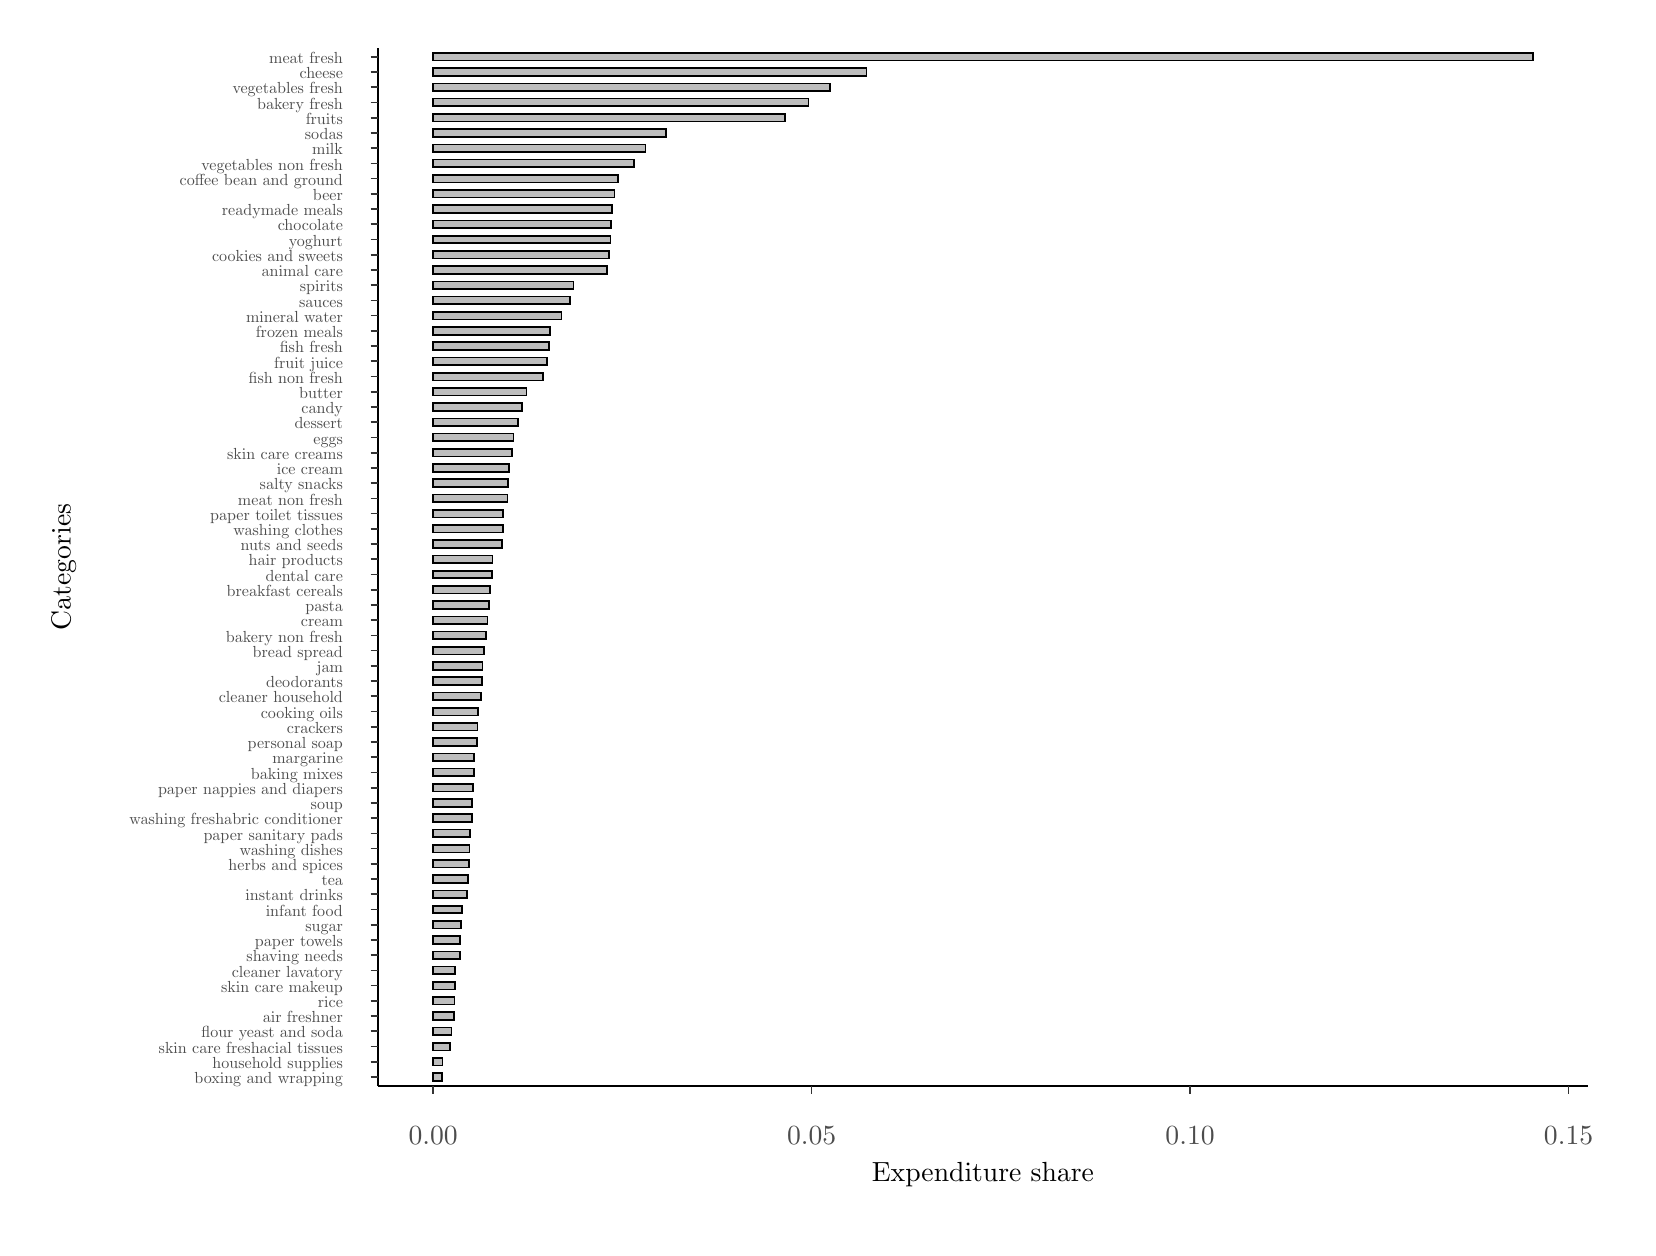
\begin{tikzpicture}[x=1pt,y=1pt]
\definecolor{fillColor}{RGB}{255,255,255}
\path[use as bounding box,fill=fillColor,fill opacity=0.00] (0,0) rectangle (578.16,433.62);
\begin{scope}
\path[clip] (  0.00,  0.00) rectangle (578.16,433.62);
\definecolor{drawColor}{RGB}{255,255,255}
\definecolor{fillColor}{RGB}{255,255,255}

\path[draw=drawColor,line width= 0.6pt,line join=round,line cap=round,fill=fillColor] (  0.00,  0.00) rectangle (578.16,433.62);
\end{scope}
\begin{scope}
\path[clip] (126.66, 51.15) rectangle (563.71,426.39);
\definecolor{drawColor}{RGB}{255,255,255}

\path[draw=drawColor,line width= 0.3pt,line join=round] (214.90, 51.15) --
	(214.90,426.39);

\path[draw=drawColor,line width= 0.3pt,line join=round] (351.66, 51.15) --
	(351.66,426.39);

\path[draw=drawColor,line width= 0.3pt,line join=round] (488.43, 51.15) --
	(488.43,426.39);
\definecolor{drawColor}{RGB}{0,0,0}
\definecolor{fillColor}{gray}{0.74}

\path[draw=drawColor,line width= 0.6pt,line cap=rect,fill=fillColor] (146.52, 75.09) rectangle (154.04, 77.84);

\path[draw=drawColor,line width= 0.6pt,line cap=rect,fill=fillColor] (146.52,344.69) rectangle (209.42,347.44);

\path[draw=drawColor,line width= 0.6pt,line cap=rect,fill=fillColor] (146.52,405.21) rectangle (282.09,407.96);

\path[draw=drawColor,line width= 0.6pt,line cap=rect,fill=fillColor] (146.52,212.64) rectangle (165.70,215.39);

\path[draw=drawColor,line width= 0.6pt,line cap=rect,fill=fillColor] (146.52,163.12) rectangle (161.16,165.87);

\path[draw=drawColor,line width= 0.6pt,line cap=rect,fill=fillColor] (146.52,372.20) rectangle (212.09,374.95);

\path[draw=drawColor,line width= 0.6pt,line cap=rect,fill=fillColor] (146.52, 53.08) rectangle (149.82, 55.83);

\path[draw=drawColor,line width= 0.6pt,line cap=rect,fill=fillColor] (146.52,207.14) rectangle (164.95,209.89);

\path[draw=drawColor,line width= 0.6pt,line cap=rect,fill=fillColor] (146.52,229.14) rectangle (167.02,231.90);

\path[draw=drawColor,line width= 0.6pt,line cap=rect,fill=fillColor] (146.52,300.67) rectangle (180.26,303.42);

\path[draw=drawColor,line width= 0.6pt,line cap=rect,fill=fillColor] (146.52,295.17) rectangle (178.63,297.92);

\path[draw=drawColor,line width= 0.6pt,line cap=rect,fill=fillColor] (146.52,416.21) rectangle (303.15,418.97);

\path[draw=drawColor,line width= 0.6pt,line cap=rect,fill=fillColor] (146.52,361.19) rectangle (210.69,363.94);

\path[draw=drawColor,line width= 0.6pt,line cap=rect,fill=fillColor] (146.52,190.63) rectangle (163.75,193.38);

\path[draw=drawColor,line width= 0.6pt,line cap=rect,fill=fillColor] (146.52, 91.59) rectangle (154.47, 94.34);

\path[draw=drawColor,line width= 0.6pt,line cap=rect,fill=fillColor] (146.52,377.70) rectangle (213.32,380.45);

\path[draw=drawColor,line width= 0.6pt,line cap=rect,fill=fillColor] (146.52,350.19) rectangle (210.12,352.94);

\path[draw=drawColor,line width= 0.6pt,line cap=rect,fill=fillColor] (146.52,185.13) rectangle (162.63,187.88);

\path[draw=drawColor,line width= 0.6pt,line cap=rect,fill=fillColor] (146.52,179.63) rectangle (162.55,182.38);

\path[draw=drawColor,line width= 0.6pt,line cap=rect,fill=fillColor] (146.52,218.14) rectangle (166.12,220.89);

\path[draw=drawColor,line width= 0.6pt,line cap=rect,fill=fillColor] (146.52,234.65) rectangle (167.81,237.40);

\path[draw=drawColor,line width= 0.6pt,line cap=rect,fill=fillColor] (146.52,196.13) rectangle (164.12,198.88);

\path[draw=drawColor,line width= 0.6pt,line cap=rect,fill=fillColor] (146.52,289.67) rectangle (177.15,292.42);

\path[draw=drawColor,line width= 0.6pt,line cap=rect,fill=fillColor] (146.52,284.17) rectangle (175.55,286.92);

\path[draw=drawColor,line width= 0.6pt,line cap=rect,fill=fillColor] (146.52,317.18) rectangle (188.43,319.93);

\path[draw=drawColor,line width= 0.6pt,line cap=rect,fill=fillColor] (146.52,306.17) rectangle (186.26,308.92);

\path[draw=drawColor,line width= 0.6pt,line cap=rect,fill=fillColor] (146.52, 69.59) rectangle (153.09, 72.34);

\path[draw=drawColor,line width= 0.6pt,line cap=rect,fill=fillColor] (146.52,322.68) rectangle (188.77,325.43);

\path[draw=drawColor,line width= 0.6pt,line cap=rect,fill=fillColor] (146.52,311.68) rectangle (187.64,314.43);

\path[draw=drawColor,line width= 0.6pt,line cap=rect,fill=fillColor] (146.52,399.71) rectangle (273.77,402.46);

\path[draw=drawColor,line width= 0.6pt,line cap=rect,fill=fillColor] (146.52,240.15) rectangle (167.98,242.90);

\path[draw=drawColor,line width= 0.6pt,line cap=rect,fill=fillColor] (146.52,130.11) rectangle (159.57,132.86);

\path[draw=drawColor,line width= 0.6pt,line cap=rect,fill=fillColor] (146.52, 58.58) rectangle (149.85, 61.33);

\path[draw=drawColor,line width= 0.6pt,line cap=rect,fill=fillColor] (146.52,273.16) rectangle (173.92,275.91);

\path[draw=drawColor,line width= 0.6pt,line cap=rect,fill=fillColor] (146.52,113.60) rectangle (156.88,116.35);

\path[draw=drawColor,line width= 0.6pt,line cap=rect,fill=fillColor] (146.52,119.10) rectangle (158.85,121.85);

\path[draw=drawColor,line width= 0.6pt,line cap=rect,fill=fillColor] (146.52,201.63) rectangle (164.37,204.39);

\path[draw=drawColor,line width= 0.6pt,line cap=rect,fill=fillColor] (146.52,168.62) rectangle (161.36,171.37);

\path[draw=drawColor,line width= 0.6pt,line cap=rect,fill=fillColor] (146.52,421.72) rectangle (543.84,424.47);

\path[draw=drawColor,line width= 0.6pt,line cap=rect,fill=fillColor] (146.52,262.16) rectangle (173.44,264.91);

\path[draw=drawColor,line width= 0.6pt,line cap=rect,fill=fillColor] (146.52,388.70) rectangle (223.21,391.46);

\path[draw=drawColor,line width= 0.6pt,line cap=rect,fill=fillColor] (146.52,328.18) rectangle (192.94,330.93);

\path[draw=drawColor,line width= 0.6pt,line cap=rect,fill=fillColor] (146.52,245.65) rectangle (171.39,248.40);

\path[draw=drawColor,line width= 0.6pt,line cap=rect,fill=fillColor] (146.52,157.62) rectangle (160.85,160.37);

\path[draw=drawColor,line width= 0.6pt,line cap=rect,fill=fillColor] (146.52,141.11) rectangle (159.86,143.86);

\path[draw=drawColor,line width= 0.6pt,line cap=rect,fill=fillColor] (146.52,256.65) rectangle (171.87,259.41);

\path[draw=drawColor,line width= 0.6pt,line cap=rect,fill=fillColor] (146.52,102.60) rectangle (156.27,105.35);

\path[draw=drawColor,line width= 0.6pt,line cap=rect,fill=fillColor] (146.52,223.64) rectangle (166.60,226.39);

\path[draw=drawColor,line width= 0.6pt,line cap=rect,fill=fillColor] (146.52,174.12) rectangle (162.27,176.88);

\path[draw=drawColor,line width= 0.6pt,line cap=rect,fill=fillColor] (146.52,366.70) rectangle (211.04,369.45);

\path[draw=drawColor,line width= 0.6pt,line cap=rect,fill=fillColor] (146.52, 80.59) rectangle (154.17, 83.34);

\path[draw=drawColor,line width= 0.6pt,line cap=rect,fill=fillColor] (146.52,267.66) rectangle (173.62,270.41);

\path[draw=drawColor,line width= 0.6pt,line cap=rect,fill=fillColor] (146.52,333.68) rectangle (196.02,336.43);

\path[draw=drawColor,line width= 0.6pt,line cap=rect,fill=fillColor] (146.52, 97.10) rectangle (156.12, 99.85);

\path[draw=drawColor,line width= 0.6pt,line cap=rect,fill=fillColor] (146.52,278.66) rectangle (174.90,281.41);

\path[draw=drawColor,line width= 0.6pt,line cap=rect,fill=fillColor] (146.52, 64.08) rectangle (152.64, 66.83);

\path[draw=drawColor,line width= 0.6pt,line cap=rect,fill=fillColor] (146.52, 86.09) rectangle (154.43, 88.84);

\path[draw=drawColor,line width= 0.6pt,line cap=rect,fill=fillColor] (146.52,394.21) rectangle (230.69,396.96);

\path[draw=drawColor,line width= 0.6pt,line cap=rect,fill=fillColor] (146.52,152.12) rectangle (160.67,154.87);

\path[draw=drawColor,line width= 0.6pt,line cap=rect,fill=fillColor] (146.52,339.19) rectangle (197.27,341.94);

\path[draw=drawColor,line width= 0.6pt,line cap=rect,fill=fillColor] (146.52,108.10) rectangle (156.59,110.85);

\path[draw=drawColor,line width= 0.6pt,line cap=rect,fill=fillColor] (146.52,124.61) rectangle (159.13,127.36);

\path[draw=drawColor,line width= 0.6pt,line cap=rect,fill=fillColor] (146.52,410.71) rectangle (289.84,413.46);

\path[draw=drawColor,line width= 0.6pt,line cap=rect,fill=fillColor] (146.52,383.20) rectangle (219.04,385.95);

\path[draw=drawColor,line width= 0.6pt,line cap=rect,fill=fillColor] (146.52,251.15) rectangle (171.73,253.90);

\path[draw=drawColor,line width= 0.6pt,line cap=rect,fill=fillColor] (146.52,135.61) rectangle (159.71,138.36);

\path[draw=drawColor,line width= 0.6pt,line cap=rect,fill=fillColor] (146.52,146.61) rectangle (160.56,149.37);

\path[draw=drawColor,line width= 0.6pt,line cap=rect,fill=fillColor] (146.52,355.69) rectangle (210.60,358.44);
\end{scope}
\begin{scope}
\path[clip] (  0.00,  0.00) rectangle (578.16,433.62);
\definecolor{drawColor}{RGB}{0,0,0}

\path[draw=drawColor,line width= 0.6pt,line join=round] (126.66, 51.15) --
	(126.66,426.39);
\end{scope}
\begin{scope}
\path[clip] (  0.00,  0.00) rectangle (578.16,433.62);
\definecolor{drawColor}{gray}{0.30}

\node[text=drawColor,anchor=base east,inner sep=0pt, outer sep=0pt, scale=  0.58] at (113.91, 52.04) {boxing and wrapping};

\node[text=drawColor,anchor=base east,inner sep=0pt, outer sep=0pt, scale=  0.58] at (113.91, 57.55) {household supplies};

\node[text=drawColor,anchor=base east,inner sep=0pt, outer sep=0pt, scale=  0.58] at (113.91, 63.05) {skin care freshacial tissues};

\node[text=drawColor,anchor=base east,inner sep=0pt, outer sep=0pt, scale=  0.58] at (113.91, 68.55) {flour yeast and soda};

\node[text=drawColor,anchor=base east,inner sep=0pt, outer sep=0pt, scale=  0.58] at (113.91, 74.05) {air freshner};

\node[text=drawColor,anchor=base east,inner sep=0pt, outer sep=0pt, scale=  0.58] at (113.91, 79.55) {rice};

\node[text=drawColor,anchor=base east,inner sep=0pt, outer sep=0pt, scale=  0.58] at (113.91, 85.06) {skin care  makeup};

\node[text=drawColor,anchor=base east,inner sep=0pt, outer sep=0pt, scale=  0.58] at (113.91, 90.56) {cleaner  lavatory};

\node[text=drawColor,anchor=base east,inner sep=0pt, outer sep=0pt, scale=  0.58] at (113.91, 96.06) {shaving needs};

\node[text=drawColor,anchor=base east,inner sep=0pt, outer sep=0pt, scale=  0.58] at (113.91,101.56) {paper  towels};

\node[text=drawColor,anchor=base east,inner sep=0pt, outer sep=0pt, scale=  0.58] at (113.91,107.06) {sugar};

\node[text=drawColor,anchor=base east,inner sep=0pt, outer sep=0pt, scale=  0.58] at (113.91,112.57) {infant food};

\node[text=drawColor,anchor=base east,inner sep=0pt, outer sep=0pt, scale=  0.58] at (113.91,118.07) {instant drinks};

\node[text=drawColor,anchor=base east,inner sep=0pt, outer sep=0pt, scale=  0.58] at (113.91,123.57) {tea};

\node[text=drawColor,anchor=base east,inner sep=0pt, outer sep=0pt, scale=  0.58] at (113.91,129.07) {herbs and spices};

\node[text=drawColor,anchor=base east,inner sep=0pt, outer sep=0pt, scale=  0.58] at (113.91,134.57) {washing  dishes};

\node[text=drawColor,anchor=base east,inner sep=0pt, outer sep=0pt, scale=  0.58] at (113.91,140.08) {paper  sanitary pads};

\node[text=drawColor,anchor=base east,inner sep=0pt, outer sep=0pt, scale=  0.58] at (113.91,145.58) {washing freshabric conditioner};

\node[text=drawColor,anchor=base east,inner sep=0pt, outer sep=0pt, scale=  0.58] at (113.91,151.08) {soup};

\node[text=drawColor,anchor=base east,inner sep=0pt, outer sep=0pt, scale=  0.58] at (113.91,156.58) {paper  nappies and diapers};

\node[text=drawColor,anchor=base east,inner sep=0pt, outer sep=0pt, scale=  0.58] at (113.91,162.08) {baking mixes};

\node[text=drawColor,anchor=base east,inner sep=0pt, outer sep=0pt, scale=  0.58] at (113.91,167.59) {margarine};

\node[text=drawColor,anchor=base east,inner sep=0pt, outer sep=0pt, scale=  0.58] at (113.91,173.09) {personal soap};

\node[text=drawColor,anchor=base east,inner sep=0pt, outer sep=0pt, scale=  0.58] at (113.91,178.59) {crackers};

\node[text=drawColor,anchor=base east,inner sep=0pt, outer sep=0pt, scale=  0.58] at (113.91,184.09) {cooking oils};

\node[text=drawColor,anchor=base east,inner sep=0pt, outer sep=0pt, scale=  0.58] at (113.91,189.60) {cleaner  household};

\node[text=drawColor,anchor=base east,inner sep=0pt, outer sep=0pt, scale=  0.58] at (113.91,195.10) {deodorants};

\node[text=drawColor,anchor=base east,inner sep=0pt, outer sep=0pt, scale=  0.58] at (113.91,200.60) {jam};

\node[text=drawColor,anchor=base east,inner sep=0pt, outer sep=0pt, scale=  0.58] at (113.91,206.10) {bread spread};

\node[text=drawColor,anchor=base east,inner sep=0pt, outer sep=0pt, scale=  0.58] at (113.91,211.60) {bakery non fresh};

\node[text=drawColor,anchor=base east,inner sep=0pt, outer sep=0pt, scale=  0.58] at (113.91,217.11) {cream};

\node[text=drawColor,anchor=base east,inner sep=0pt, outer sep=0pt, scale=  0.58] at (113.91,222.61) {pasta};

\node[text=drawColor,anchor=base east,inner sep=0pt, outer sep=0pt, scale=  0.58] at (113.91,228.11) {breakfast cereals};

\node[text=drawColor,anchor=base east,inner sep=0pt, outer sep=0pt, scale=  0.58] at (113.91,233.61) {dental care};

\node[text=drawColor,anchor=base east,inner sep=0pt, outer sep=0pt, scale=  0.58] at (113.91,239.11) {hair products};

\node[text=drawColor,anchor=base east,inner sep=0pt, outer sep=0pt, scale=  0.58] at (113.91,244.62) {nuts and seeds};

\node[text=drawColor,anchor=base east,inner sep=0pt, outer sep=0pt, scale=  0.58] at (113.91,250.12) {washing  clothes};

\node[text=drawColor,anchor=base east,inner sep=0pt, outer sep=0pt, scale=  0.58] at (113.91,255.62) {paper  toilet tissues};

\node[text=drawColor,anchor=base east,inner sep=0pt, outer sep=0pt, scale=  0.58] at (113.91,261.12) {meat non fresh};

\node[text=drawColor,anchor=base east,inner sep=0pt, outer sep=0pt, scale=  0.58] at (113.91,266.62) {salty snacks};

\node[text=drawColor,anchor=base east,inner sep=0pt, outer sep=0pt, scale=  0.58] at (113.91,272.13) {ice cream};

\node[text=drawColor,anchor=base east,inner sep=0pt, outer sep=0pt, scale=  0.58] at (113.91,277.63) {skin care  creams};

\node[text=drawColor,anchor=base east,inner sep=0pt, outer sep=0pt, scale=  0.58] at (113.91,283.13) {eggs};

\node[text=drawColor,anchor=base east,inner sep=0pt, outer sep=0pt, scale=  0.58] at (113.91,288.63) {dessert};

\node[text=drawColor,anchor=base east,inner sep=0pt, outer sep=0pt, scale=  0.58] at (113.91,294.13) {candy};

\node[text=drawColor,anchor=base east,inner sep=0pt, outer sep=0pt, scale=  0.58] at (113.91,299.64) {butter};

\node[text=drawColor,anchor=base east,inner sep=0pt, outer sep=0pt, scale=  0.58] at (113.91,305.14) {fish non fresh};

\node[text=drawColor,anchor=base east,inner sep=0pt, outer sep=0pt, scale=  0.58] at (113.91,310.64) {fruit juice};

\node[text=drawColor,anchor=base east,inner sep=0pt, outer sep=0pt, scale=  0.58] at (113.91,316.14) {fish fresh};

\node[text=drawColor,anchor=base east,inner sep=0pt, outer sep=0pt, scale=  0.58] at (113.91,321.64) {frozen meals};

\node[text=drawColor,anchor=base east,inner sep=0pt, outer sep=0pt, scale=  0.58] at (113.91,327.15) {mineral water};

\node[text=drawColor,anchor=base east,inner sep=0pt, outer sep=0pt, scale=  0.58] at (113.91,332.65) {sauces};

\node[text=drawColor,anchor=base east,inner sep=0pt, outer sep=0pt, scale=  0.58] at (113.91,338.15) {spirits};

\node[text=drawColor,anchor=base east,inner sep=0pt, outer sep=0pt, scale=  0.58] at (113.91,343.65) {animal care};

\node[text=drawColor,anchor=base east,inner sep=0pt, outer sep=0pt, scale=  0.58] at (113.91,349.15) {cookies and sweets};

\node[text=drawColor,anchor=base east,inner sep=0pt, outer sep=0pt, scale=  0.58] at (113.91,354.66) {yoghurt};

\node[text=drawColor,anchor=base east,inner sep=0pt, outer sep=0pt, scale=  0.58] at (113.91,360.16) {chocolate};

\node[text=drawColor,anchor=base east,inner sep=0pt, outer sep=0pt, scale=  0.58] at (113.91,365.66) {readymade meals};

\node[text=drawColor,anchor=base east,inner sep=0pt, outer sep=0pt, scale=  0.58] at (113.91,371.16) {beer};

\node[text=drawColor,anchor=base east,inner sep=0pt, outer sep=0pt, scale=  0.58] at (113.91,376.66) {coffee  bean and ground};

\node[text=drawColor,anchor=base east,inner sep=0pt, outer sep=0pt, scale=  0.58] at (113.91,382.17) {vegetables non fresh};

\node[text=drawColor,anchor=base east,inner sep=0pt, outer sep=0pt, scale=  0.58] at (113.91,387.67) {milk};

\node[text=drawColor,anchor=base east,inner sep=0pt, outer sep=0pt, scale=  0.58] at (113.91,393.17) {sodas};

\node[text=drawColor,anchor=base east,inner sep=0pt, outer sep=0pt, scale=  0.58] at (113.91,398.67) {fruits};

\node[text=drawColor,anchor=base east,inner sep=0pt, outer sep=0pt, scale=  0.58] at (113.91,404.17) {bakery fresh};

\node[text=drawColor,anchor=base east,inner sep=0pt, outer sep=0pt, scale=  0.58] at (113.91,409.68) {vegetables fresh};

\node[text=drawColor,anchor=base east,inner sep=0pt, outer sep=0pt, scale=  0.58] at (113.91,415.18) {cheese};

\node[text=drawColor,anchor=base east,inner sep=0pt, outer sep=0pt, scale=  0.58] at (113.91,420.68) {meat fresh};
\end{scope}
\begin{scope}
\path[clip] (  0.00,  0.00) rectangle (578.16,433.62);
\definecolor{drawColor}{gray}{0.20}

\path[draw=drawColor,line width= 0.6pt,line join=round] (123.91, 54.45) --
	(126.66, 54.45);

\path[draw=drawColor,line width= 0.6pt,line join=round] (123.91, 59.96) --
	(126.66, 59.96);

\path[draw=drawColor,line width= 0.6pt,line join=round] (123.91, 65.46) --
	(126.66, 65.46);

\path[draw=drawColor,line width= 0.6pt,line join=round] (123.91, 70.96) --
	(126.66, 70.96);

\path[draw=drawColor,line width= 0.6pt,line join=round] (123.91, 76.46) --
	(126.66, 76.46);

\path[draw=drawColor,line width= 0.6pt,line join=round] (123.91, 81.97) --
	(126.66, 81.97);

\path[draw=drawColor,line width= 0.6pt,line join=round] (123.91, 87.47) --
	(126.66, 87.47);

\path[draw=drawColor,line width= 0.6pt,line join=round] (123.91, 92.97) --
	(126.66, 92.97);

\path[draw=drawColor,line width= 0.6pt,line join=round] (123.91, 98.47) --
	(126.66, 98.47);

\path[draw=drawColor,line width= 0.6pt,line join=round] (123.91,103.97) --
	(126.66,103.97);

\path[draw=drawColor,line width= 0.6pt,line join=round] (123.91,109.48) --
	(126.66,109.48);

\path[draw=drawColor,line width= 0.6pt,line join=round] (123.91,114.98) --
	(126.66,114.98);

\path[draw=drawColor,line width= 0.6pt,line join=round] (123.91,120.48) --
	(126.66,120.48);

\path[draw=drawColor,line width= 0.6pt,line join=round] (123.91,125.98) --
	(126.66,125.98);

\path[draw=drawColor,line width= 0.6pt,line join=round] (123.91,131.48) --
	(126.66,131.48);

\path[draw=drawColor,line width= 0.6pt,line join=round] (123.91,136.99) --
	(126.66,136.99);

\path[draw=drawColor,line width= 0.6pt,line join=round] (123.91,142.49) --
	(126.66,142.49);

\path[draw=drawColor,line width= 0.6pt,line join=round] (123.91,147.99) --
	(126.66,147.99);

\path[draw=drawColor,line width= 0.6pt,line join=round] (123.91,153.49) --
	(126.66,153.49);

\path[draw=drawColor,line width= 0.6pt,line join=round] (123.91,158.99) --
	(126.66,158.99);

\path[draw=drawColor,line width= 0.6pt,line join=round] (123.91,164.50) --
	(126.66,164.50);

\path[draw=drawColor,line width= 0.6pt,line join=round] (123.91,170.00) --
	(126.66,170.00);

\path[draw=drawColor,line width= 0.6pt,line join=round] (123.91,175.50) --
	(126.66,175.50);

\path[draw=drawColor,line width= 0.6pt,line join=round] (123.91,181.00) --
	(126.66,181.00);

\path[draw=drawColor,line width= 0.6pt,line join=round] (123.91,186.50) --
	(126.66,186.50);

\path[draw=drawColor,line width= 0.6pt,line join=round] (123.91,192.01) --
	(126.66,192.01);

\path[draw=drawColor,line width= 0.6pt,line join=round] (123.91,197.51) --
	(126.66,197.51);

\path[draw=drawColor,line width= 0.6pt,line join=round] (123.91,203.01) --
	(126.66,203.01);

\path[draw=drawColor,line width= 0.6pt,line join=round] (123.91,208.51) --
	(126.66,208.51);

\path[draw=drawColor,line width= 0.6pt,line join=round] (123.91,214.01) --
	(126.66,214.01);

\path[draw=drawColor,line width= 0.6pt,line join=round] (123.91,219.52) --
	(126.66,219.52);

\path[draw=drawColor,line width= 0.6pt,line join=round] (123.91,225.02) --
	(126.66,225.02);

\path[draw=drawColor,line width= 0.6pt,line join=round] (123.91,230.52) --
	(126.66,230.52);

\path[draw=drawColor,line width= 0.6pt,line join=round] (123.91,236.02) --
	(126.66,236.02);

\path[draw=drawColor,line width= 0.6pt,line join=round] (123.91,241.52) --
	(126.66,241.52);

\path[draw=drawColor,line width= 0.6pt,line join=round] (123.91,247.03) --
	(126.66,247.03);

\path[draw=drawColor,line width= 0.6pt,line join=round] (123.91,252.53) --
	(126.66,252.53);

\path[draw=drawColor,line width= 0.6pt,line join=round] (123.91,258.03) --
	(126.66,258.03);

\path[draw=drawColor,line width= 0.6pt,line join=round] (123.91,263.53) --
	(126.66,263.53);

\path[draw=drawColor,line width= 0.6pt,line join=round] (123.91,269.03) --
	(126.66,269.03);

\path[draw=drawColor,line width= 0.6pt,line join=round] (123.91,274.54) --
	(126.66,274.54);

\path[draw=drawColor,line width= 0.6pt,line join=round] (123.91,280.04) --
	(126.66,280.04);

\path[draw=drawColor,line width= 0.6pt,line join=round] (123.91,285.54) --
	(126.66,285.54);

\path[draw=drawColor,line width= 0.6pt,line join=round] (123.91,291.04) --
	(126.66,291.04);

\path[draw=drawColor,line width= 0.6pt,line join=round] (123.91,296.54) --
	(126.66,296.54);

\path[draw=drawColor,line width= 0.6pt,line join=round] (123.91,302.05) --
	(126.66,302.05);

\path[draw=drawColor,line width= 0.6pt,line join=round] (123.91,307.55) --
	(126.66,307.55);

\path[draw=drawColor,line width= 0.6pt,line join=round] (123.91,313.05) --
	(126.66,313.05);

\path[draw=drawColor,line width= 0.6pt,line join=round] (123.91,318.55) --
	(126.66,318.55);

\path[draw=drawColor,line width= 0.6pt,line join=round] (123.91,324.05) --
	(126.66,324.05);

\path[draw=drawColor,line width= 0.6pt,line join=round] (123.91,329.56) --
	(126.66,329.56);

\path[draw=drawColor,line width= 0.6pt,line join=round] (123.91,335.06) --
	(126.66,335.06);

\path[draw=drawColor,line width= 0.6pt,line join=round] (123.91,340.56) --
	(126.66,340.56);

\path[draw=drawColor,line width= 0.6pt,line join=round] (123.91,346.06) --
	(126.66,346.06);

\path[draw=drawColor,line width= 0.6pt,line join=round] (123.91,351.57) --
	(126.66,351.57);

\path[draw=drawColor,line width= 0.6pt,line join=round] (123.91,357.07) --
	(126.66,357.07);

\path[draw=drawColor,line width= 0.6pt,line join=round] (123.91,362.57) --
	(126.66,362.57);

\path[draw=drawColor,line width= 0.6pt,line join=round] (123.91,368.07) --
	(126.66,368.07);

\path[draw=drawColor,line width= 0.6pt,line join=round] (123.91,373.57) --
	(126.66,373.57);

\path[draw=drawColor,line width= 0.6pt,line join=round] (123.91,379.08) --
	(126.66,379.08);

\path[draw=drawColor,line width= 0.6pt,line join=round] (123.91,384.58) --
	(126.66,384.58);

\path[draw=drawColor,line width= 0.6pt,line join=round] (123.91,390.08) --
	(126.66,390.08);

\path[draw=drawColor,line width= 0.6pt,line join=round] (123.91,395.58) --
	(126.66,395.58);

\path[draw=drawColor,line width= 0.6pt,line join=round] (123.91,401.08) --
	(126.66,401.08);

\path[draw=drawColor,line width= 0.6pt,line join=round] (123.91,406.59) --
	(126.66,406.59);

\path[draw=drawColor,line width= 0.6pt,line join=round] (123.91,412.09) --
	(126.66,412.09);

\path[draw=drawColor,line width= 0.6pt,line join=round] (123.91,417.59) --
	(126.66,417.59);

\path[draw=drawColor,line width= 0.6pt,line join=round] (123.91,423.09) --
	(126.66,423.09);
\end{scope}
\begin{scope}
\path[clip] (  0.00,  0.00) rectangle (578.16,433.62);
\definecolor{drawColor}{RGB}{0,0,0}

\path[draw=drawColor,line width= 0.6pt,line join=round] (126.66, 51.15) --
	(563.71, 51.15);
\end{scope}
\begin{scope}
\path[clip] (  0.00,  0.00) rectangle (578.16,433.62);
\definecolor{drawColor}{gray}{0.20}

\path[draw=drawColor,line width= 0.6pt,line join=round] (146.52, 48.40) --
	(146.52, 51.15);

\path[draw=drawColor,line width= 0.6pt,line join=round] (283.28, 48.40) --
	(283.28, 51.15);

\path[draw=drawColor,line width= 0.6pt,line join=round] (420.04, 48.40) --
	(420.04, 51.15);

\path[draw=drawColor,line width= 0.6pt,line join=round] (556.81, 48.40) --
	(556.81, 51.15);
\end{scope}
\begin{scope}
\path[clip] (  0.00,  0.00) rectangle (578.16,433.62);
\definecolor{drawColor}{gray}{0.30}

\node[text=drawColor,anchor=base,inner sep=0pt, outer sep=0pt, scale=  1.00] at (146.52, 30.14) {0.00};

\node[text=drawColor,anchor=base,inner sep=0pt, outer sep=0pt, scale=  1.00] at (283.28, 30.14) {0.05};

\node[text=drawColor,anchor=base,inner sep=0pt, outer sep=0pt, scale=  1.00] at (420.04, 30.14) {0.10};

\node[text=drawColor,anchor=base,inner sep=0pt, outer sep=0pt, scale=  1.00] at (556.81, 30.14) {0.15};
\end{scope}
\begin{scope}
\path[clip] (  0.00,  0.00) rectangle (578.16,433.62);
\definecolor{drawColor}{RGB}{0,0,0}

\node[text=drawColor,anchor=base,inner sep=0pt, outer sep=0pt, scale=  1.00] at (345.18, 16.79) {Expenditure share};
\end{scope}
\begin{scope}
\path[clip] (  0.00,  0.00) rectangle (578.16,433.62);
\definecolor{drawColor}{RGB}{0,0,0}

\node[text=drawColor,rotate= 90.00,anchor=base,inner sep=0pt, outer sep=0pt, scale=  1.00] at ( 15.49,238.77) {Categories};
\end{scope}
\end{tikzpicture}
}
	\parbox{\textwidth}{
	\begin{spacing}{1} 
		{\footnotesize} 
        \textit{Notes}: The graph plots the average expenditure share across the product categories. We compute this by pooling expenditure across the countries for each year and then averaging over years. 
	\end{spacing}}
\end{figure}

\subsection{Households}
\begin{table}[H]
	\centering		
	\caption{Size Distribution by number of UPCs}
    \label{tab: app_households_excluded}
	\begin{spacing}{1.1}
        \begin{tabular}{lrrrrrr} \toprule
            & \multicolumn{3}{c}{Belgium} & \multicolumn{3}{c}{France} \\ 
                \cmidrule(lr){2-4} \cmidrule(lr){5-7} 
            &   Households & Transactions & Exp. share &
                Households & Transactions & Exp. share\\ \midrule
		    Sample&3,215&4,599,884&0.84&7,008&8,102,354&0.58\\
Excluded&1,663&887,629&0.16&11,138&5,777,336&0.42\\
\midrule

            & \multicolumn{3}{c}{Germany} & \multicolumn{3}{c}{Netherlands} \\ 
                \cmidrule(lr){2-4} \cmidrule(lr){5-7} 
            &   Households & Transactions & Exp. share &
                Households & Transactions & Exp. share\\ \midrule
           Sample&23,348&28,412,861&0.88&8,424&13,103,004&0.91\\
Excluded&13,523&4,037,140&0.12&2,395&1,307,629&0.09\\
\bottomrule

	    \end{tabular}
    \end{spacing}
    \parbox{\textwidth}{
        \begin{spacing}{1} 
            {\footnotesize 
            \textit{Notes}: This table shows for each country (1) the number of households, (2) the number of transactions and (3) the share in total expenditure in the group of included and excluded households.}
        \end{spacing}}
\end{table}
\begin{figure}[H]
   \centering
   \caption{Expenditure per year}
   \label{fig: app_data_households_exp_year}
   \begin{subfigure}[t]{.49\textwidth}
		\centering
        \caption{Belgium}
        \scalebox{0.45}{% Created by tikzDevice version 0.12.3.1 on 2022-07-29 15:13:23
% !TEX encoding = UTF-8 Unicode
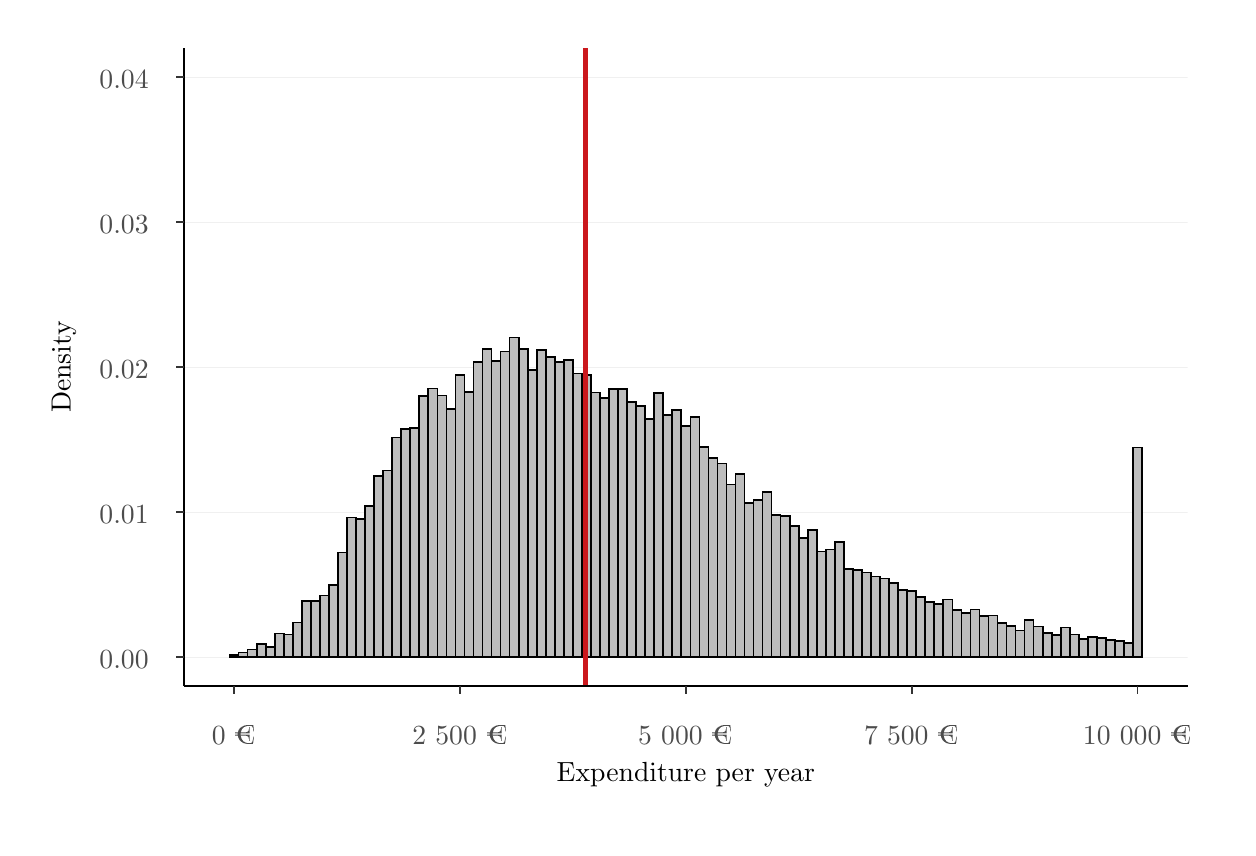
\begin{tikzpicture}[x=1pt,y=1pt]
\definecolor{fillColor}{RGB}{255,255,255}
\path[use as bounding box,fill=fillColor,fill opacity=0.00] (0,0) rectangle (433.62,289.08);
\begin{scope}
\path[clip] (  0.00,  0.00) rectangle (433.62,289.08);
\definecolor{drawColor}{RGB}{255,255,255}
\definecolor{fillColor}{RGB}{255,255,255}

\path[draw=drawColor,line width= 0.6pt,line join=round,line cap=round,fill=fillColor] ( -0.00,  0.00) rectangle (433.62,289.08);
\end{scope}
\begin{scope}
\path[clip] ( 56.47, 51.15) rectangle (419.17,281.85);
\definecolor{drawColor}{RGB}{255,255,255}

\path[draw=drawColor,line width= 0.3pt,line join=round] ( 56.47, 87.86) --
	(419.17, 87.86);

\path[draw=drawColor,line width= 0.3pt,line join=round] ( 56.47,140.29) --
	(419.17,140.29);

\path[draw=drawColor,line width= 0.3pt,line join=round] ( 56.47,192.72) --
	(419.17,192.72);

\path[draw=drawColor,line width= 0.3pt,line join=round] ( 56.47,245.15) --
	(419.17,245.15);

\path[draw=drawColor,line width= 0.3pt,line join=round] (115.39, 51.15) --
	(115.39,281.85);

\path[draw=drawColor,line width= 0.3pt,line join=round] (197.01, 51.15) --
	(197.01,281.85);

\path[draw=drawColor,line width= 0.3pt,line join=round] (278.62, 51.15) --
	(278.62,281.85);

\path[draw=drawColor,line width= 0.3pt,line join=round] (360.24, 51.15) --
	(360.24,281.85);
\definecolor{drawColor}{gray}{0.94}

\path[draw=drawColor,line width= 0.1pt,line join=round] ( 56.47, 61.64) --
	(419.17, 61.64);

\path[draw=drawColor,line width= 0.1pt,line join=round] ( 56.47,114.07) --
	(419.17,114.07);

\path[draw=drawColor,line width= 0.1pt,line join=round] ( 56.47,166.50) --
	(419.17,166.50);

\path[draw=drawColor,line width= 0.1pt,line join=round] ( 56.47,218.93) --
	(419.17,218.93);

\path[draw=drawColor,line width= 0.1pt,line join=round] ( 56.47,271.37) --
	(419.17,271.37);
\definecolor{drawColor}{RGB}{0,0,0}
\definecolor{fillColor}{gray}{0.74}

\path[draw=drawColor,line width= 0.6pt,line cap=rect,fill=fillColor] ( 72.95, 61.64) rectangle ( 76.22, 62.28);

\path[draw=drawColor,line width= 0.6pt,line cap=rect,fill=fillColor] ( 76.22, 61.64) rectangle ( 79.48, 63.24);

\path[draw=drawColor,line width= 0.6pt,line cap=rect,fill=fillColor] ( 79.48, 61.64) rectangle ( 82.75, 64.36);

\path[draw=drawColor,line width= 0.6pt,line cap=rect,fill=fillColor] ( 82.75, 61.64) rectangle ( 86.01, 66.45);

\path[draw=drawColor,line width= 0.6pt,line cap=rect,fill=fillColor] ( 86.01, 61.64) rectangle ( 89.28, 65.32);

\path[draw=drawColor,line width= 0.6pt,line cap=rect,fill=fillColor] ( 89.28, 61.64) rectangle ( 92.54, 70.13);

\path[draw=drawColor,line width= 0.6pt,line cap=rect,fill=fillColor] ( 92.54, 61.64) rectangle ( 95.80, 69.81);

\path[draw=drawColor,line width= 0.6pt,line cap=rect,fill=fillColor] ( 95.80, 61.64) rectangle ( 99.07, 74.14);

\path[draw=drawColor,line width= 0.6pt,line cap=rect,fill=fillColor] ( 99.07, 61.64) rectangle (102.33, 81.99);

\path[draw=drawColor,line width= 0.6pt,line cap=rect,fill=fillColor] (102.33, 61.64) rectangle (105.60, 81.83);

\path[draw=drawColor,line width= 0.6pt,line cap=rect,fill=fillColor] (105.60, 61.64) rectangle (108.86, 83.91);

\path[draw=drawColor,line width= 0.6pt,line cap=rect,fill=fillColor] (108.86, 61.64) rectangle (112.13, 87.59);

\path[draw=drawColor,line width= 0.6pt,line cap=rect,fill=fillColor] (112.13, 61.64) rectangle (115.39, 99.45);

\path[draw=drawColor,line width= 0.6pt,line cap=rect,fill=fillColor] (115.39, 61.64) rectangle (118.66,112.10);

\path[draw=drawColor,line width= 0.6pt,line cap=rect,fill=fillColor] (118.66, 61.64) rectangle (121.92,111.46);

\path[draw=drawColor,line width= 0.6pt,line cap=rect,fill=fillColor] (121.92, 61.64) rectangle (125.19,116.27);

\path[draw=drawColor,line width= 0.6pt,line cap=rect,fill=fillColor] (125.19, 61.64) rectangle (128.45,127.00);

\path[draw=drawColor,line width= 0.6pt,line cap=rect,fill=fillColor] (128.45, 61.64) rectangle (131.72,129.08);

\path[draw=drawColor,line width= 0.6pt,line cap=rect,fill=fillColor] (131.72, 61.64) rectangle (134.98,140.94);

\path[draw=drawColor,line width= 0.6pt,line cap=rect,fill=fillColor] (134.98, 61.64) rectangle (138.24,143.98);

\path[draw=drawColor,line width= 0.6pt,line cap=rect,fill=fillColor] (138.24, 61.64) rectangle (141.51,144.46);

\path[draw=drawColor,line width= 0.6pt,line cap=rect,fill=fillColor] (141.51, 61.64) rectangle (144.77,156.00);

\path[draw=drawColor,line width= 0.6pt,line cap=rect,fill=fillColor] (144.77, 61.64) rectangle (148.04,158.72);

\path[draw=drawColor,line width= 0.6pt,line cap=rect,fill=fillColor] (148.04, 61.64) rectangle (151.30,156.16);

\path[draw=drawColor,line width= 0.6pt,line cap=rect,fill=fillColor] (151.30, 61.64) rectangle (154.57,151.19);

\path[draw=drawColor,line width= 0.6pt,line cap=rect,fill=fillColor] (154.57, 61.64) rectangle (157.83,163.53);

\path[draw=drawColor,line width= 0.6pt,line cap=rect,fill=fillColor] (157.83, 61.64) rectangle (161.10,157.44);

\path[draw=drawColor,line width= 0.6pt,line cap=rect,fill=fillColor] (161.10, 61.64) rectangle (164.36,168.33);

\path[draw=drawColor,line width= 0.6pt,line cap=rect,fill=fillColor] (164.36, 61.64) rectangle (167.63,172.98);

\path[draw=drawColor,line width= 0.6pt,line cap=rect,fill=fillColor] (167.63, 61.64) rectangle (170.89,168.65);

\path[draw=drawColor,line width= 0.6pt,line cap=rect,fill=fillColor] (170.89, 61.64) rectangle (174.16,172.02);

\path[draw=drawColor,line width= 0.6pt,line cap=rect,fill=fillColor] (174.16, 61.64) rectangle (177.42,177.14);

\path[draw=drawColor,line width= 0.6pt,line cap=rect,fill=fillColor] (177.42, 61.64) rectangle (180.68,172.98);

\path[draw=drawColor,line width= 0.6pt,line cap=rect,fill=fillColor] (180.68, 61.64) rectangle (183.95,165.45);

\path[draw=drawColor,line width= 0.6pt,line cap=rect,fill=fillColor] (183.95, 61.64) rectangle (187.21,172.66);

\path[draw=drawColor,line width= 0.6pt,line cap=rect,fill=fillColor] (187.21, 61.64) rectangle (190.48,170.09);

\path[draw=drawColor,line width= 0.6pt,line cap=rect,fill=fillColor] (190.48, 61.64) rectangle (193.74,168.17);

\path[draw=drawColor,line width= 0.6pt,line cap=rect,fill=fillColor] (193.74, 61.64) rectangle (197.01,168.97);

\path[draw=drawColor,line width= 0.6pt,line cap=rect,fill=fillColor] (197.01, 61.64) rectangle (200.27,164.17);

\path[draw=drawColor,line width= 0.6pt,line cap=rect,fill=fillColor] (200.27, 61.64) rectangle (203.54,163.69);

\path[draw=drawColor,line width= 0.6pt,line cap=rect,fill=fillColor] (203.54, 61.64) rectangle (206.80,157.28);

\path[draw=drawColor,line width= 0.6pt,line cap=rect,fill=fillColor] (206.80, 61.64) rectangle (210.07,155.20);

\path[draw=drawColor,line width= 0.6pt,line cap=rect,fill=fillColor] (210.07, 61.64) rectangle (213.33,158.56);

\path[draw=drawColor,line width= 0.6pt,line cap=rect,fill=fillColor] (213.33, 61.64) rectangle (216.60,158.40);

\path[draw=drawColor,line width= 0.6pt,line cap=rect,fill=fillColor] (216.60, 61.64) rectangle (219.86,153.91);

\path[draw=drawColor,line width= 0.6pt,line cap=rect,fill=fillColor] (219.86, 61.64) rectangle (223.13,152.47);

\path[draw=drawColor,line width= 0.6pt,line cap=rect,fill=fillColor] (223.13, 61.64) rectangle (226.39,147.67);

\path[draw=drawColor,line width= 0.6pt,line cap=rect,fill=fillColor] (226.39, 61.64) rectangle (229.65,156.96);

\path[draw=drawColor,line width= 0.6pt,line cap=rect,fill=fillColor] (229.65, 61.64) rectangle (232.92,149.11);

\path[draw=drawColor,line width= 0.6pt,line cap=rect,fill=fillColor] (232.92, 61.64) rectangle (236.18,150.87);

\path[draw=drawColor,line width= 0.6pt,line cap=rect,fill=fillColor] (236.18, 61.64) rectangle (239.45,145.10);

\path[draw=drawColor,line width= 0.6pt,line cap=rect,fill=fillColor] (239.45, 61.64) rectangle (242.71,148.31);

\path[draw=drawColor,line width= 0.6pt,line cap=rect,fill=fillColor] (242.71, 61.64) rectangle (245.98,137.57);

\path[draw=drawColor,line width= 0.6pt,line cap=rect,fill=fillColor] (245.98, 61.64) rectangle (249.24,133.57);

\path[draw=drawColor,line width= 0.6pt,line cap=rect,fill=fillColor] (249.24, 61.64) rectangle (252.51,131.65);

\path[draw=drawColor,line width= 0.6pt,line cap=rect,fill=fillColor] (252.51, 61.64) rectangle (255.77,123.96);

\path[draw=drawColor,line width= 0.6pt,line cap=rect,fill=fillColor] (255.77, 61.64) rectangle (259.04,127.80);

\path[draw=drawColor,line width= 0.6pt,line cap=rect,fill=fillColor] (259.04, 61.64) rectangle (262.30,117.23);

\path[draw=drawColor,line width= 0.6pt,line cap=rect,fill=fillColor] (262.30, 61.64) rectangle (265.57,118.51);

\path[draw=drawColor,line width= 0.6pt,line cap=rect,fill=fillColor] (265.57, 61.64) rectangle (268.83,121.39);

\path[draw=drawColor,line width= 0.6pt,line cap=rect,fill=fillColor] (268.83, 61.64) rectangle (272.09,112.90);

\path[draw=drawColor,line width= 0.6pt,line cap=rect,fill=fillColor] (272.09, 61.64) rectangle (275.36,112.74);

\path[draw=drawColor,line width= 0.6pt,line cap=rect,fill=fillColor] (275.36, 61.64) rectangle (278.62,108.90);

\path[draw=drawColor,line width= 0.6pt,line cap=rect,fill=fillColor] (278.62, 61.64) rectangle (281.89,104.57);

\path[draw=drawColor,line width= 0.6pt,line cap=rect,fill=fillColor] (281.89, 61.64) rectangle (285.15,107.62);

\path[draw=drawColor,line width= 0.6pt,line cap=rect,fill=fillColor] (285.15, 61.64) rectangle (288.42, 99.77);

\path[draw=drawColor,line width= 0.6pt,line cap=rect,fill=fillColor] (288.42, 61.64) rectangle (291.68,100.57);

\path[draw=drawColor,line width= 0.6pt,line cap=rect,fill=fillColor] (291.68, 61.64) rectangle (294.95,103.13);

\path[draw=drawColor,line width= 0.6pt,line cap=rect,fill=fillColor] (294.95, 61.64) rectangle (298.21, 93.52);

\path[draw=drawColor,line width= 0.6pt,line cap=rect,fill=fillColor] (298.21, 61.64) rectangle (301.48, 93.20);

\path[draw=drawColor,line width= 0.6pt,line cap=rect,fill=fillColor] (301.48, 61.64) rectangle (304.74, 92.24);

\path[draw=drawColor,line width= 0.6pt,line cap=rect,fill=fillColor] (304.74, 61.64) rectangle (308.01, 90.80);

\path[draw=drawColor,line width= 0.6pt,line cap=rect,fill=fillColor] (308.01, 61.64) rectangle (311.27, 90.00);

\path[draw=drawColor,line width= 0.6pt,line cap=rect,fill=fillColor] (311.27, 61.64) rectangle (314.53, 88.39);

\path[draw=drawColor,line width= 0.6pt,line cap=rect,fill=fillColor] (314.53, 61.64) rectangle (317.80, 85.99);

\path[draw=drawColor,line width= 0.6pt,line cap=rect,fill=fillColor] (317.80, 61.64) rectangle (321.06, 85.51);

\path[draw=drawColor,line width= 0.6pt,line cap=rect,fill=fillColor] (321.06, 61.64) rectangle (324.33, 83.27);

\path[draw=drawColor,line width= 0.6pt,line cap=rect,fill=fillColor] (324.33, 61.64) rectangle (327.59, 81.50);

\path[draw=drawColor,line width= 0.6pt,line cap=rect,fill=fillColor] (327.59, 61.64) rectangle (330.86, 80.86);

\path[draw=drawColor,line width= 0.6pt,line cap=rect,fill=fillColor] (330.86, 61.64) rectangle (334.12, 82.47);

\path[draw=drawColor,line width= 0.6pt,line cap=rect,fill=fillColor] (334.12, 61.64) rectangle (337.39, 78.62);

\path[draw=drawColor,line width= 0.6pt,line cap=rect,fill=fillColor] (337.39, 61.64) rectangle (340.65, 77.66);

\path[draw=drawColor,line width= 0.6pt,line cap=rect,fill=fillColor] (340.65, 61.64) rectangle (343.92, 78.78);

\path[draw=drawColor,line width= 0.6pt,line cap=rect,fill=fillColor] (343.92, 61.64) rectangle (347.18, 76.54);

\path[draw=drawColor,line width= 0.6pt,line cap=rect,fill=fillColor] (347.18, 61.64) rectangle (350.45, 76.70);

\path[draw=drawColor,line width= 0.6pt,line cap=rect,fill=fillColor] (350.45, 61.64) rectangle (353.71, 73.98);

\path[draw=drawColor,line width= 0.6pt,line cap=rect,fill=fillColor] (353.71, 61.64) rectangle (356.97, 72.85);

\path[draw=drawColor,line width= 0.6pt,line cap=rect,fill=fillColor] (356.97, 61.64) rectangle (360.24, 71.25);

\path[draw=drawColor,line width= 0.6pt,line cap=rect,fill=fillColor] (360.24, 61.64) rectangle (363.50, 74.94);

\path[draw=drawColor,line width= 0.6pt,line cap=rect,fill=fillColor] (363.50, 61.64) rectangle (366.77, 72.69);

\path[draw=drawColor,line width= 0.6pt,line cap=rect,fill=fillColor] (366.77, 61.64) rectangle (370.03, 70.45);

\path[draw=drawColor,line width= 0.6pt,line cap=rect,fill=fillColor] (370.03, 61.64) rectangle (373.30, 69.65);

\path[draw=drawColor,line width= 0.6pt,line cap=rect,fill=fillColor] (373.30, 61.64) rectangle (376.56, 72.37);

\path[draw=drawColor,line width= 0.6pt,line cap=rect,fill=fillColor] (376.56, 61.64) rectangle (379.83, 69.81);

\path[draw=drawColor,line width= 0.6pt,line cap=rect,fill=fillColor] (379.83, 61.64) rectangle (383.09, 68.21);

\path[draw=drawColor,line width= 0.6pt,line cap=rect,fill=fillColor] (383.09, 61.64) rectangle (386.36, 68.85);

\path[draw=drawColor,line width= 0.6pt,line cap=rect,fill=fillColor] (386.36, 61.64) rectangle (389.62, 68.53);

\path[draw=drawColor,line width= 0.6pt,line cap=rect,fill=fillColor] (389.62, 61.64) rectangle (392.89, 67.73);

\path[draw=drawColor,line width= 0.6pt,line cap=rect,fill=fillColor] (392.89, 61.64) rectangle (396.15, 67.41);

\path[draw=drawColor,line width= 0.6pt,line cap=rect,fill=fillColor] (396.15, 61.64) rectangle (399.41, 66.77);

\path[draw=drawColor,line width= 0.6pt,line cap=rect,fill=fillColor] (399.41, 61.64) rectangle (402.68,137.41);
\definecolor{drawColor}{RGB}{203,24,29}

\path[draw=drawColor,line width= 1.7pt,line join=round] (201.67, 51.15) -- (201.67,281.85);
\end{scope}
\begin{scope}
\path[clip] (  0.00,  0.00) rectangle (433.62,289.08);
\definecolor{drawColor}{RGB}{0,0,0}

\path[draw=drawColor,line width= 0.6pt,line join=round] ( 56.47, 51.15) --
	( 56.47,281.85);
\end{scope}
\begin{scope}
\path[clip] (  0.00,  0.00) rectangle (433.62,289.08);
\definecolor{drawColor}{gray}{0.30}

\node[text=drawColor,anchor=base east,inner sep=0pt, outer sep=0pt, scale=  1.00] at ( 43.72, 57.51) {0.00};

\node[text=drawColor,anchor=base east,inner sep=0pt, outer sep=0pt, scale=  1.00] at ( 43.72,109.94) {0.01};

\node[text=drawColor,anchor=base east,inner sep=0pt, outer sep=0pt, scale=  1.00] at ( 43.72,162.37) {0.02};

\node[text=drawColor,anchor=base east,inner sep=0pt, outer sep=0pt, scale=  1.00] at ( 43.72,214.80) {0.03};

\node[text=drawColor,anchor=base east,inner sep=0pt, outer sep=0pt, scale=  1.00] at ( 43.72,267.23) {0.04};
\end{scope}
\begin{scope}
\path[clip] (  0.00,  0.00) rectangle (433.62,289.08);
\definecolor{drawColor}{gray}{0.20}

\path[draw=drawColor,line width= 0.6pt,line join=round] ( 53.72, 61.64) --
	( 56.47, 61.64);

\path[draw=drawColor,line width= 0.6pt,line join=round] ( 53.72,114.07) --
	( 56.47,114.07);

\path[draw=drawColor,line width= 0.6pt,line join=round] ( 53.72,166.50) --
	( 56.47,166.50);

\path[draw=drawColor,line width= 0.6pt,line join=round] ( 53.72,218.93) --
	( 56.47,218.93);

\path[draw=drawColor,line width= 0.6pt,line join=round] ( 53.72,271.37) --
	( 56.47,271.37);
\end{scope}
\begin{scope}
\path[clip] (  0.00,  0.00) rectangle (433.62,289.08);
\definecolor{drawColor}{RGB}{0,0,0}

\path[draw=drawColor,line width= 0.6pt,line join=round] ( 56.47, 51.15) --
	(419.17, 51.15);
\end{scope}
\begin{scope}
\path[clip] (  0.00,  0.00) rectangle (433.62,289.08);
\definecolor{drawColor}{gray}{0.20}

\path[draw=drawColor,line width= 0.6pt,line join=round] ( 74.58, 48.40) --
	( 74.58, 51.15);

\path[draw=drawColor,line width= 0.6pt,line join=round] (156.20, 48.40) --
	(156.20, 51.15);

\path[draw=drawColor,line width= 0.6pt,line join=round] (237.82, 48.40) --
	(237.82, 51.15);

\path[draw=drawColor,line width= 0.6pt,line join=round] (319.43, 48.40) --
	(319.43, 51.15);

\path[draw=drawColor,line width= 0.6pt,line join=round] (401.05, 48.40) --
	(401.05, 51.15);
\end{scope}
\begin{scope}
\path[clip] (  0.00,  0.00) rectangle (433.62,289.08);
\definecolor{drawColor}{gray}{0.30}

\node[text=drawColor,anchor=base,inner sep=0pt, outer sep=0pt, scale=  1.00] at ( 74.58, 30.14) {0 €};

\node[text=drawColor,anchor=base,inner sep=0pt, outer sep=0pt, scale=  1.00] at (156.20, 30.14) {2 500 €};

\node[text=drawColor,anchor=base,inner sep=0pt, outer sep=0pt, scale=  1.00] at (237.82, 30.14) {5 000 €};

\node[text=drawColor,anchor=base,inner sep=0pt, outer sep=0pt, scale=  1.00] at (319.43, 30.14) {7 500 €};

\node[text=drawColor,anchor=base,inner sep=0pt, outer sep=0pt, scale=  1.00] at (401.05, 30.14) {10 000 €};
\end{scope}
\begin{scope}
\path[clip] (  0.00,  0.00) rectangle (433.62,289.08);
\definecolor{drawColor}{RGB}{0,0,0}

\node[text=drawColor,anchor=base,inner sep=0pt, outer sep=0pt, scale=  1.00] at (237.82, 16.79) {Expenditure per year};
\end{scope}
\begin{scope}
\path[clip] (  0.00,  0.00) rectangle (433.62,289.08);
\definecolor{drawColor}{RGB}{0,0,0}

\node[text=drawColor,rotate= 90.00,anchor=base,inner sep=0pt, outer sep=0pt, scale=  1.00] at ( 15.49,166.50) {Density};
\end{scope}
\end{tikzpicture}
}
    \end{subfigure}
    \begin{subfigure}[t]{.49\textwidth}
		\centering
        \caption{France}
        \scalebox{0.45}{% Created by tikzDevice version 0.12.3.1 on 2022-07-29 15:13:35
% !TEX encoding = UTF-8 Unicode
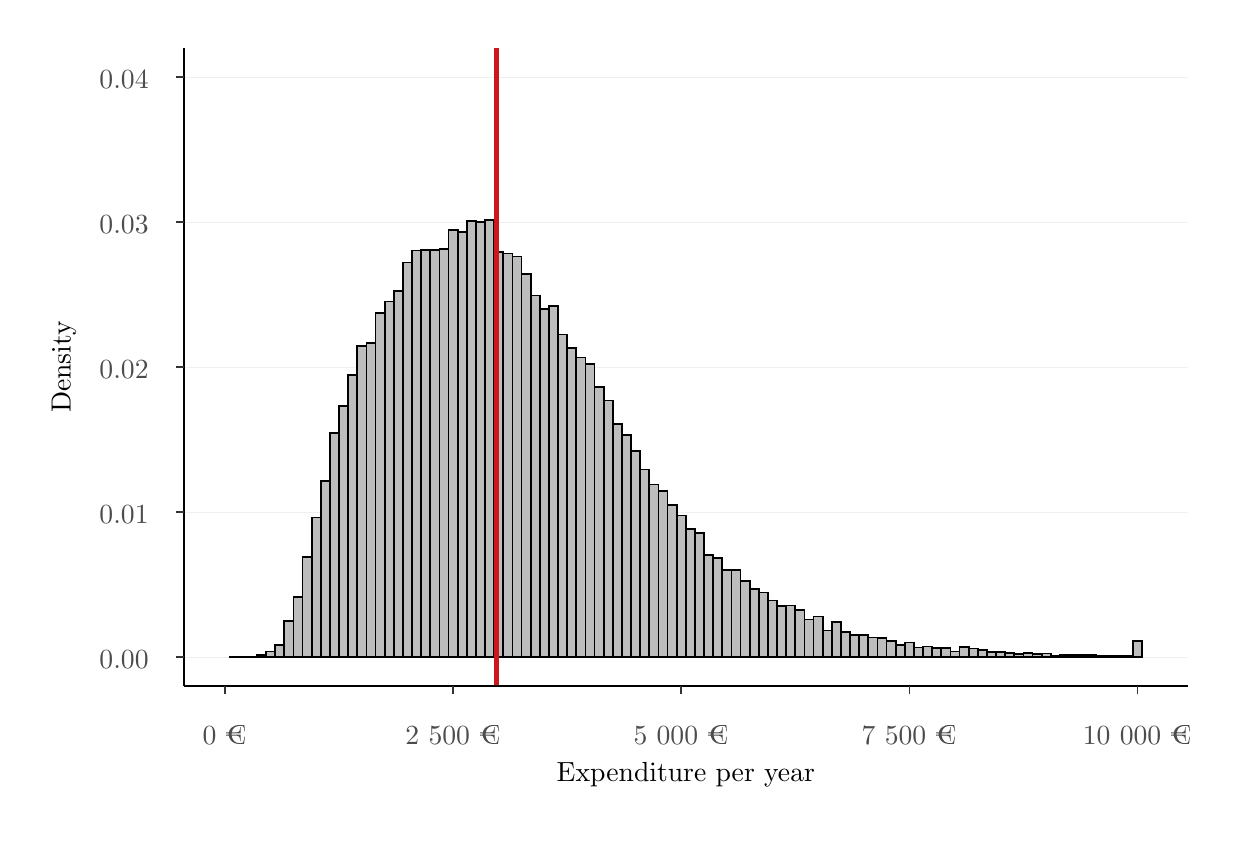
\begin{tikzpicture}[x=1pt,y=1pt]
\definecolor{fillColor}{RGB}{255,255,255}
\path[use as bounding box,fill=fillColor,fill opacity=0.00] (0,0) rectangle (433.62,289.08);
\begin{scope}
\path[clip] (  0.00,  0.00) rectangle (433.62,289.08);
\definecolor{drawColor}{RGB}{255,255,255}
\definecolor{fillColor}{RGB}{255,255,255}

\path[draw=drawColor,line width= 0.6pt,line join=round,line cap=round,fill=fillColor] ( -0.00,  0.00) rectangle (433.62,289.08);
\end{scope}
\begin{scope}
\path[clip] ( 56.47, 51.15) rectangle (419.17,281.85);
\definecolor{drawColor}{RGB}{255,255,255}

\path[draw=drawColor,line width= 0.3pt,line join=round] ( 56.47, 87.86) --
	(419.17, 87.86);

\path[draw=drawColor,line width= 0.3pt,line join=round] ( 56.47,140.29) --
	(419.17,140.29);

\path[draw=drawColor,line width= 0.3pt,line join=round] ( 56.47,192.72) --
	(419.17,192.72);

\path[draw=drawColor,line width= 0.3pt,line join=round] ( 56.47,245.15) --
	(419.17,245.15);

\path[draw=drawColor,line width= 0.3pt,line join=round] (112.52, 51.15) --
	(112.52,281.85);

\path[draw=drawColor,line width= 0.3pt,line join=round] (194.95, 51.15) --
	(194.95,281.85);

\path[draw=drawColor,line width= 0.3pt,line join=round] (277.38, 51.15) --
	(277.38,281.85);

\path[draw=drawColor,line width= 0.3pt,line join=round] (359.82, 51.15) --
	(359.82,281.85);
\definecolor{drawColor}{gray}{0.94}

\path[draw=drawColor,line width= 0.1pt,line join=round] ( 56.47, 61.64) --
	(419.17, 61.64);

\path[draw=drawColor,line width= 0.1pt,line join=round] ( 56.47,114.07) --
	(419.17,114.07);

\path[draw=drawColor,line width= 0.1pt,line join=round] ( 56.47,166.50) --
	(419.17,166.50);

\path[draw=drawColor,line width= 0.1pt,line join=round] ( 56.47,218.93) --
	(419.17,218.93);

\path[draw=drawColor,line width= 0.1pt,line join=round] ( 56.47,271.37) --
	(419.17,271.37);
\definecolor{drawColor}{RGB}{0,0,0}
\definecolor{fillColor}{gray}{0.74}

\path[draw=drawColor,line width= 0.6pt,line cap=rect,fill=fillColor] ( 72.95, 61.64) rectangle ( 76.25, 61.71);

\path[draw=drawColor,line width= 0.6pt,line cap=rect,fill=fillColor] ( 76.25, 61.64) rectangle ( 79.55, 61.64);

\path[draw=drawColor,line width= 0.6pt,line cap=rect,fill=fillColor] ( 79.55, 61.64) rectangle ( 82.84, 61.79);

\path[draw=drawColor,line width= 0.6pt,line cap=rect,fill=fillColor] ( 82.84, 61.64) rectangle ( 86.14, 62.31);

\path[draw=drawColor,line width= 0.6pt,line cap=rect,fill=fillColor] ( 86.14, 61.64) rectangle ( 89.44, 63.66);

\path[draw=drawColor,line width= 0.6pt,line cap=rect,fill=fillColor] ( 89.44, 61.64) rectangle ( 92.74, 65.97);

\path[draw=drawColor,line width= 0.6pt,line cap=rect,fill=fillColor] ( 92.74, 61.64) rectangle ( 96.03, 74.79);

\path[draw=drawColor,line width= 0.6pt,line cap=rect,fill=fillColor] ( 96.03, 61.64) rectangle ( 99.33, 83.46);

\path[draw=drawColor,line width= 0.6pt,line cap=rect,fill=fillColor] ( 99.33, 61.64) rectangle (102.63, 97.89);

\path[draw=drawColor,line width= 0.6pt,line cap=rect,fill=fillColor] (102.63, 61.64) rectangle (105.92,112.02);

\path[draw=drawColor,line width= 0.6pt,line cap=rect,fill=fillColor] (105.92, 61.64) rectangle (109.22,125.17);

\path[draw=drawColor,line width= 0.6pt,line cap=rect,fill=fillColor] (109.22, 61.64) rectangle (112.52,142.51);

\path[draw=drawColor,line width= 0.6pt,line cap=rect,fill=fillColor] (112.52, 61.64) rectangle (115.82,152.38);

\path[draw=drawColor,line width= 0.6pt,line cap=rect,fill=fillColor] (115.82, 61.64) rectangle (119.11,163.66);

\path[draw=drawColor,line width= 0.6pt,line cap=rect,fill=fillColor] (119.11, 61.64) rectangle (122.41,174.13);

\path[draw=drawColor,line width= 0.6pt,line cap=rect,fill=fillColor] (122.41, 61.64) rectangle (125.71,175.10);

\path[draw=drawColor,line width= 0.6pt,line cap=rect,fill=fillColor] (125.71, 61.64) rectangle (129.01,185.93);

\path[draw=drawColor,line width= 0.6pt,line cap=rect,fill=fillColor] (129.01, 61.64) rectangle (132.30,190.19);

\path[draw=drawColor,line width= 0.6pt,line cap=rect,fill=fillColor] (132.30, 61.64) rectangle (135.60,193.93);

\path[draw=drawColor,line width= 0.6pt,line cap=rect,fill=fillColor] (135.60, 61.64) rectangle (138.90,204.25);

\path[draw=drawColor,line width= 0.6pt,line cap=rect,fill=fillColor] (138.90, 61.64) rectangle (142.19,208.51);

\path[draw=drawColor,line width= 0.6pt,line cap=rect,fill=fillColor] (142.19, 61.64) rectangle (145.49,208.81);

\path[draw=drawColor,line width= 0.6pt,line cap=rect,fill=fillColor] (145.49, 61.64) rectangle (148.79,208.73);

\path[draw=drawColor,line width= 0.6pt,line cap=rect,fill=fillColor] (148.79, 61.64) rectangle (152.09,209.10);

\path[draw=drawColor,line width= 0.6pt,line cap=rect,fill=fillColor] (152.09, 61.64) rectangle (155.38,215.98);

\path[draw=drawColor,line width= 0.6pt,line cap=rect,fill=fillColor] (155.38, 61.64) rectangle (158.68,215.16);

\path[draw=drawColor,line width= 0.6pt,line cap=rect,fill=fillColor] (158.68, 61.64) rectangle (161.98,219.12);

\path[draw=drawColor,line width= 0.6pt,line cap=rect,fill=fillColor] (161.98, 61.64) rectangle (165.28,218.75);

\path[draw=drawColor,line width= 0.6pt,line cap=rect,fill=fillColor] (165.28, 61.64) rectangle (168.57,219.64);

\path[draw=drawColor,line width= 0.6pt,line cap=rect,fill=fillColor] (168.57, 61.64) rectangle (171.87,207.98);

\path[draw=drawColor,line width= 0.6pt,line cap=rect,fill=fillColor] (171.87, 61.64) rectangle (175.17,207.53);

\path[draw=drawColor,line width= 0.6pt,line cap=rect,fill=fillColor] (175.17, 61.64) rectangle (178.46,206.41);

\path[draw=drawColor,line width= 0.6pt,line cap=rect,fill=fillColor] (178.46, 61.64) rectangle (181.76,200.14);

\path[draw=drawColor,line width= 0.6pt,line cap=rect,fill=fillColor] (181.76, 61.64) rectangle (185.06,192.29);

\path[draw=drawColor,line width= 0.6pt,line cap=rect,fill=fillColor] (185.06, 61.64) rectangle (188.36,187.35);

\path[draw=drawColor,line width= 0.6pt,line cap=rect,fill=fillColor] (188.36, 61.64) rectangle (191.65,188.55);

\path[draw=drawColor,line width= 0.6pt,line cap=rect,fill=fillColor] (191.65, 61.64) rectangle (194.95,178.16);

\path[draw=drawColor,line width= 0.6pt,line cap=rect,fill=fillColor] (194.95, 61.64) rectangle (198.25,173.30);

\path[draw=drawColor,line width= 0.6pt,line cap=rect,fill=fillColor] (198.25, 61.64) rectangle (201.55,169.94);

\path[draw=drawColor,line width= 0.6pt,line cap=rect,fill=fillColor] (201.55, 61.64) rectangle (204.84,167.55);

\path[draw=drawColor,line width= 0.6pt,line cap=rect,fill=fillColor] (204.84, 61.64) rectangle (208.14,159.25);

\path[draw=drawColor,line width= 0.6pt,line cap=rect,fill=fillColor] (208.14, 61.64) rectangle (211.44,154.32);

\path[draw=drawColor,line width= 0.6pt,line cap=rect,fill=fillColor] (211.44, 61.64) rectangle (214.73,145.95);

\path[draw=drawColor,line width= 0.6pt,line cap=rect,fill=fillColor] (214.73, 61.64) rectangle (218.03,141.84);

\path[draw=drawColor,line width= 0.6pt,line cap=rect,fill=fillColor] (218.03, 61.64) rectangle (221.33,136.08);

\path[draw=drawColor,line width= 0.6pt,line cap=rect,fill=fillColor] (221.33, 61.64) rectangle (224.63,129.43);

\path[draw=drawColor,line width= 0.6pt,line cap=rect,fill=fillColor] (224.63, 61.64) rectangle (227.92,123.97);

\path[draw=drawColor,line width= 0.6pt,line cap=rect,fill=fillColor] (227.92, 61.64) rectangle (231.22,121.66);

\path[draw=drawColor,line width= 0.6pt,line cap=rect,fill=fillColor] (231.22, 61.64) rectangle (234.52,116.50);

\path[draw=drawColor,line width= 0.6pt,line cap=rect,fill=fillColor] (234.52, 61.64) rectangle (237.82,112.76);

\path[draw=drawColor,line width= 0.6pt,line cap=rect,fill=fillColor] (237.82, 61.64) rectangle (241.11,107.98);

\path[draw=drawColor,line width= 0.6pt,line cap=rect,fill=fillColor] (241.11, 61.64) rectangle (244.41,106.48);

\path[draw=drawColor,line width= 0.6pt,line cap=rect,fill=fillColor] (244.41, 61.64) rectangle (247.71, 98.64);

\path[draw=drawColor,line width= 0.6pt,line cap=rect,fill=fillColor] (247.71, 61.64) rectangle (251.00, 97.52);

\path[draw=drawColor,line width= 0.6pt,line cap=rect,fill=fillColor] (251.00, 61.64) rectangle (254.30, 93.11);

\path[draw=drawColor,line width= 0.6pt,line cap=rect,fill=fillColor] (254.30, 61.64) rectangle (257.60, 93.18);

\path[draw=drawColor,line width= 0.6pt,line cap=rect,fill=fillColor] (257.60, 61.64) rectangle (260.90, 89.14);

\path[draw=drawColor,line width= 0.6pt,line cap=rect,fill=fillColor] (260.90, 61.64) rectangle (264.19, 86.30);

\path[draw=drawColor,line width= 0.6pt,line cap=rect,fill=fillColor] (264.19, 61.64) rectangle (267.49, 85.03);

\path[draw=drawColor,line width= 0.6pt,line cap=rect,fill=fillColor] (267.49, 61.64) rectangle (270.79, 82.12);

\path[draw=drawColor,line width= 0.6pt,line cap=rect,fill=fillColor] (270.79, 61.64) rectangle (274.09, 80.03);

\path[draw=drawColor,line width= 0.6pt,line cap=rect,fill=fillColor] (274.09, 61.64) rectangle (277.38, 80.25);

\path[draw=drawColor,line width= 0.6pt,line cap=rect,fill=fillColor] (277.38, 61.64) rectangle (280.68, 78.61);

\path[draw=drawColor,line width= 0.6pt,line cap=rect,fill=fillColor] (280.68, 61.64) rectangle (283.98, 75.17);

\path[draw=drawColor,line width= 0.6pt,line cap=rect,fill=fillColor] (283.98, 61.64) rectangle (287.27, 76.29);

\path[draw=drawColor,line width= 0.6pt,line cap=rect,fill=fillColor] (287.27, 61.64) rectangle (290.57, 71.21);

\path[draw=drawColor,line width= 0.6pt,line cap=rect,fill=fillColor] (290.57, 61.64) rectangle (293.87, 74.20);

\path[draw=drawColor,line width= 0.6pt,line cap=rect,fill=fillColor] (293.87, 61.64) rectangle (297.17, 70.61);

\path[draw=drawColor,line width= 0.6pt,line cap=rect,fill=fillColor] (297.17, 61.64) rectangle (300.46, 69.56);

\path[draw=drawColor,line width= 0.6pt,line cap=rect,fill=fillColor] (300.46, 61.64) rectangle (303.76, 69.56);

\path[draw=drawColor,line width= 0.6pt,line cap=rect,fill=fillColor] (303.76, 61.64) rectangle (307.06, 68.67);

\path[draw=drawColor,line width= 0.6pt,line cap=rect,fill=fillColor] (307.06, 61.64) rectangle (310.36, 68.44);

\path[draw=drawColor,line width= 0.6pt,line cap=rect,fill=fillColor] (310.36, 61.64) rectangle (313.65, 67.54);

\path[draw=drawColor,line width= 0.6pt,line cap=rect,fill=fillColor] (313.65, 61.64) rectangle (316.95, 66.12);

\path[draw=drawColor,line width= 0.6pt,line cap=rect,fill=fillColor] (316.95, 61.64) rectangle (320.25, 66.95);

\path[draw=drawColor,line width= 0.6pt,line cap=rect,fill=fillColor] (320.25, 61.64) rectangle (323.55, 65.15);

\path[draw=drawColor,line width= 0.6pt,line cap=rect,fill=fillColor] (323.55, 61.64) rectangle (326.84, 65.45);

\path[draw=drawColor,line width= 0.6pt,line cap=rect,fill=fillColor] (326.84, 61.64) rectangle (330.14, 64.93);

\path[draw=drawColor,line width= 0.6pt,line cap=rect,fill=fillColor] (330.14, 61.64) rectangle (333.44, 64.85);

\path[draw=drawColor,line width= 0.6pt,line cap=rect,fill=fillColor] (333.44, 61.64) rectangle (336.73, 63.66);

\path[draw=drawColor,line width= 0.6pt,line cap=rect,fill=fillColor] (336.73, 61.64) rectangle (340.03, 65.38);

\path[draw=drawColor,line width= 0.6pt,line cap=rect,fill=fillColor] (340.03, 61.64) rectangle (343.33, 64.70);

\path[draw=drawColor,line width= 0.6pt,line cap=rect,fill=fillColor] (343.33, 61.64) rectangle (346.63, 64.11);

\path[draw=drawColor,line width= 0.6pt,line cap=rect,fill=fillColor] (346.63, 61.64) rectangle (349.92, 63.51);

\path[draw=drawColor,line width= 0.6pt,line cap=rect,fill=fillColor] (349.92, 61.64) rectangle (353.22, 63.36);

\path[draw=drawColor,line width= 0.6pt,line cap=rect,fill=fillColor] (353.22, 61.64) rectangle (356.52, 63.06);

\path[draw=drawColor,line width= 0.6pt,line cap=rect,fill=fillColor] (356.52, 61.64) rectangle (359.82, 62.76);

\path[draw=drawColor,line width= 0.6pt,line cap=rect,fill=fillColor] (359.82, 61.64) rectangle (363.11, 63.06);

\path[draw=drawColor,line width= 0.6pt,line cap=rect,fill=fillColor] (363.11, 61.64) rectangle (366.41, 62.76);

\path[draw=drawColor,line width= 0.6pt,line cap=rect,fill=fillColor] (366.41, 61.64) rectangle (369.71, 62.91);

\path[draw=drawColor,line width= 0.6pt,line cap=rect,fill=fillColor] (369.71, 61.64) rectangle (373.00, 62.09);

\path[draw=drawColor,line width= 0.6pt,line cap=rect,fill=fillColor] (373.00, 61.64) rectangle (376.30, 62.39);

\path[draw=drawColor,line width= 0.6pt,line cap=rect,fill=fillColor] (376.30, 61.64) rectangle (379.60, 62.39);

\path[draw=drawColor,line width= 0.6pt,line cap=rect,fill=fillColor] (379.60, 61.64) rectangle (382.90, 62.39);

\path[draw=drawColor,line width= 0.6pt,line cap=rect,fill=fillColor] (382.90, 61.64) rectangle (386.19, 62.39);

\path[draw=drawColor,line width= 0.6pt,line cap=rect,fill=fillColor] (386.19, 61.64) rectangle (389.49, 62.24);

\path[draw=drawColor,line width= 0.6pt,line cap=rect,fill=fillColor] (389.49, 61.64) rectangle (392.79, 62.09);

\path[draw=drawColor,line width= 0.6pt,line cap=rect,fill=fillColor] (392.79, 61.64) rectangle (396.09, 61.94);

\path[draw=drawColor,line width= 0.6pt,line cap=rect,fill=fillColor] (396.09, 61.64) rectangle (399.38, 62.24);

\path[draw=drawColor,line width= 0.6pt,line cap=rect,fill=fillColor] (399.38, 61.64) rectangle (402.68, 67.39);
\definecolor{drawColor}{RGB}{203,24,29}

\path[draw=drawColor,line width= 1.7pt,line join=round] (169.33, 51.15) -- (169.33,281.85);
\end{scope}
\begin{scope}
\path[clip] (  0.00,  0.00) rectangle (433.62,289.08);
\definecolor{drawColor}{RGB}{0,0,0}

\path[draw=drawColor,line width= 0.6pt,line join=round] ( 56.47, 51.15) --
	( 56.47,281.85);
\end{scope}
\begin{scope}
\path[clip] (  0.00,  0.00) rectangle (433.62,289.08);
\definecolor{drawColor}{gray}{0.30}

\node[text=drawColor,anchor=base east,inner sep=0pt, outer sep=0pt, scale=  1.00] at ( 43.72, 57.51) {0.00};

\node[text=drawColor,anchor=base east,inner sep=0pt, outer sep=0pt, scale=  1.00] at ( 43.72,109.94) {0.01};

\node[text=drawColor,anchor=base east,inner sep=0pt, outer sep=0pt, scale=  1.00] at ( 43.72,162.37) {0.02};

\node[text=drawColor,anchor=base east,inner sep=0pt, outer sep=0pt, scale=  1.00] at ( 43.72,214.80) {0.03};

\node[text=drawColor,anchor=base east,inner sep=0pt, outer sep=0pt, scale=  1.00] at ( 43.72,267.23) {0.04};
\end{scope}
\begin{scope}
\path[clip] (  0.00,  0.00) rectangle (433.62,289.08);
\definecolor{drawColor}{gray}{0.20}

\path[draw=drawColor,line width= 0.6pt,line join=round] ( 53.72, 61.64) --
	( 56.47, 61.64);

\path[draw=drawColor,line width= 0.6pt,line join=round] ( 53.72,114.07) --
	( 56.47,114.07);

\path[draw=drawColor,line width= 0.6pt,line join=round] ( 53.72,166.50) --
	( 56.47,166.50);

\path[draw=drawColor,line width= 0.6pt,line join=round] ( 53.72,218.93) --
	( 56.47,218.93);

\path[draw=drawColor,line width= 0.6pt,line join=round] ( 53.72,271.37) --
	( 56.47,271.37);
\end{scope}
\begin{scope}
\path[clip] (  0.00,  0.00) rectangle (433.62,289.08);
\definecolor{drawColor}{RGB}{0,0,0}

\path[draw=drawColor,line width= 0.6pt,line join=round] ( 56.47, 51.15) --
	(419.17, 51.15);
\end{scope}
\begin{scope}
\path[clip] (  0.00,  0.00) rectangle (433.62,289.08);
\definecolor{drawColor}{gray}{0.20}

\path[draw=drawColor,line width= 0.6pt,line join=round] ( 71.30, 48.40) --
	( 71.30, 51.15);

\path[draw=drawColor,line width= 0.6pt,line join=round] (153.74, 48.40) --
	(153.74, 51.15);

\path[draw=drawColor,line width= 0.6pt,line join=round] (236.17, 48.40) --
	(236.17, 51.15);

\path[draw=drawColor,line width= 0.6pt,line join=round] (318.60, 48.40) --
	(318.60, 51.15);

\path[draw=drawColor,line width= 0.6pt,line join=round] (401.03, 48.40) --
	(401.03, 51.15);
\end{scope}
\begin{scope}
\path[clip] (  0.00,  0.00) rectangle (433.62,289.08);
\definecolor{drawColor}{gray}{0.30}

\node[text=drawColor,anchor=base,inner sep=0pt, outer sep=0pt, scale=  1.00] at ( 71.30, 30.14) {0 €};

\node[text=drawColor,anchor=base,inner sep=0pt, outer sep=0pt, scale=  1.00] at (153.74, 30.14) {2 500 €};

\node[text=drawColor,anchor=base,inner sep=0pt, outer sep=0pt, scale=  1.00] at (236.17, 30.14) {5 000 €};

\node[text=drawColor,anchor=base,inner sep=0pt, outer sep=0pt, scale=  1.00] at (318.60, 30.14) {7 500 €};

\node[text=drawColor,anchor=base,inner sep=0pt, outer sep=0pt, scale=  1.00] at (401.03, 30.14) {10 000 €};
\end{scope}
\begin{scope}
\path[clip] (  0.00,  0.00) rectangle (433.62,289.08);
\definecolor{drawColor}{RGB}{0,0,0}

\node[text=drawColor,anchor=base,inner sep=0pt, outer sep=0pt, scale=  1.00] at (237.82, 16.79) {Expenditure per year};
\end{scope}
\begin{scope}
\path[clip] (  0.00,  0.00) rectangle (433.62,289.08);
\definecolor{drawColor}{RGB}{0,0,0}

\node[text=drawColor,rotate= 90.00,anchor=base,inner sep=0pt, outer sep=0pt, scale=  1.00] at ( 15.49,166.50) {Density};
\end{scope}
\end{tikzpicture}
}
    \end{subfigure}\\
    \begin{subfigure}[t]{.49\textwidth}
		\centering
        \caption{Germany}
        \scalebox{0.45}{% Created by tikzDevice version 0.12.3.1 on 2022-07-29 15:13:35
% !TEX encoding = UTF-8 Unicode
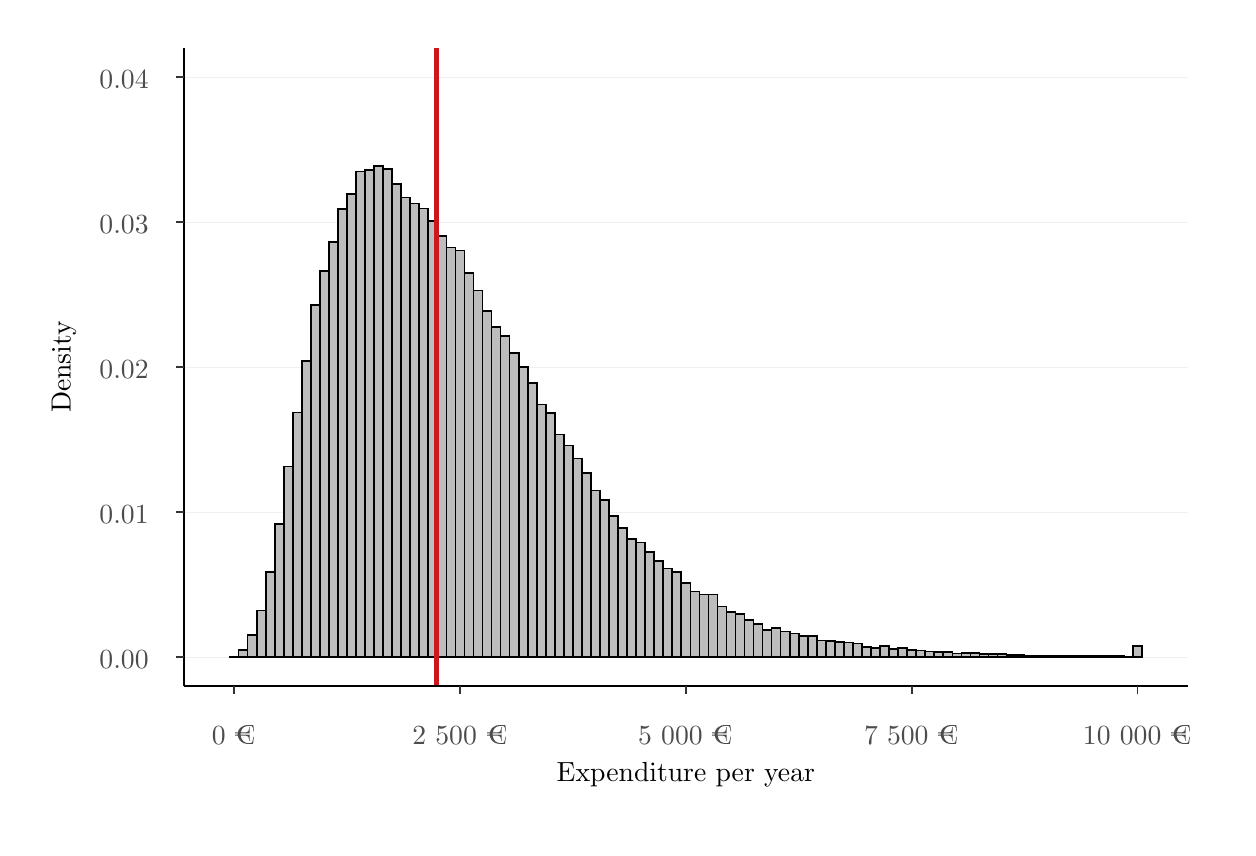
\begin{tikzpicture}[x=1pt,y=1pt]
\definecolor{fillColor}{RGB}{255,255,255}
\path[use as bounding box,fill=fillColor,fill opacity=0.00] (0,0) rectangle (433.62,289.08);
\begin{scope}
\path[clip] (  0.00,  0.00) rectangle (433.62,289.08);
\definecolor{drawColor}{RGB}{255,255,255}
\definecolor{fillColor}{RGB}{255,255,255}

\path[draw=drawColor,line width= 0.6pt,line join=round,line cap=round,fill=fillColor] ( -0.00,  0.00) rectangle (433.62,289.08);
\end{scope}
\begin{scope}
\path[clip] ( 56.47, 51.15) rectangle (419.17,281.85);
\definecolor{drawColor}{RGB}{255,255,255}

\path[draw=drawColor,line width= 0.3pt,line join=round] ( 56.47, 87.86) --
	(419.17, 87.86);

\path[draw=drawColor,line width= 0.3pt,line join=round] ( 56.47,140.29) --
	(419.17,140.29);

\path[draw=drawColor,line width= 0.3pt,line join=round] ( 56.47,192.72) --
	(419.17,192.72);

\path[draw=drawColor,line width= 0.3pt,line join=round] ( 56.47,245.15) --
	(419.17,245.15);

\path[draw=drawColor,line width= 0.3pt,line join=round] (115.39, 51.15) --
	(115.39,281.85);

\path[draw=drawColor,line width= 0.3pt,line join=round] (197.01, 51.15) --
	(197.01,281.85);

\path[draw=drawColor,line width= 0.3pt,line join=round] (278.62, 51.15) --
	(278.62,281.85);

\path[draw=drawColor,line width= 0.3pt,line join=round] (360.24, 51.15) --
	(360.24,281.85);
\definecolor{drawColor}{gray}{0.94}

\path[draw=drawColor,line width= 0.1pt,line join=round] ( 56.47, 61.64) --
	(419.17, 61.64);

\path[draw=drawColor,line width= 0.1pt,line join=round] ( 56.47,114.07) --
	(419.17,114.07);

\path[draw=drawColor,line width= 0.1pt,line join=round] ( 56.47,166.50) --
	(419.17,166.50);

\path[draw=drawColor,line width= 0.1pt,line join=round] ( 56.47,218.93) --
	(419.17,218.93);

\path[draw=drawColor,line width= 0.1pt,line join=round] ( 56.47,271.37) --
	(419.17,271.37);
\definecolor{drawColor}{RGB}{0,0,0}
\definecolor{fillColor}{gray}{0.74}

\path[draw=drawColor,line width= 0.6pt,line cap=rect,fill=fillColor] ( 72.95, 61.64) rectangle ( 76.22, 61.91);

\path[draw=drawColor,line width= 0.6pt,line cap=rect,fill=fillColor] ( 76.22, 61.64) rectangle ( 79.48, 64.16);

\path[draw=drawColor,line width= 0.6pt,line cap=rect,fill=fillColor] ( 79.48, 61.64) rectangle ( 82.75, 69.72);

\path[draw=drawColor,line width= 0.6pt,line cap=rect,fill=fillColor] ( 82.75, 61.64) rectangle ( 86.01, 78.42);

\path[draw=drawColor,line width= 0.6pt,line cap=rect,fill=fillColor] ( 86.01, 61.64) rectangle ( 89.28, 92.27);

\path[draw=drawColor,line width= 0.6pt,line cap=rect,fill=fillColor] ( 89.28, 61.64) rectangle ( 92.54,109.70);

\path[draw=drawColor,line width= 0.6pt,line cap=rect,fill=fillColor] ( 92.54, 61.64) rectangle ( 95.80,130.54);

\path[draw=drawColor,line width= 0.6pt,line cap=rect,fill=fillColor] ( 95.80, 61.64) rectangle ( 99.07,150.05);

\path[draw=drawColor,line width= 0.6pt,line cap=rect,fill=fillColor] ( 99.07, 61.64) rectangle (102.33,168.74);

\path[draw=drawColor,line width= 0.6pt,line cap=rect,fill=fillColor] (102.33, 61.64) rectangle (105.60,188.86);

\path[draw=drawColor,line width= 0.6pt,line cap=rect,fill=fillColor] (105.60, 61.64) rectangle (108.86,201.14);

\path[draw=drawColor,line width= 0.6pt,line cap=rect,fill=fillColor] (108.86, 61.64) rectangle (112.13,211.52);

\path[draw=drawColor,line width= 0.6pt,line cap=rect,fill=fillColor] (112.13, 61.64) rectangle (115.39,223.60);

\path[draw=drawColor,line width= 0.6pt,line cap=rect,fill=fillColor] (115.39, 61.64) rectangle (118.66,228.94);

\path[draw=drawColor,line width= 0.6pt,line cap=rect,fill=fillColor] (118.66, 61.64) rectangle (121.92,237.14);

\path[draw=drawColor,line width= 0.6pt,line cap=rect,fill=fillColor] (121.92, 61.64) rectangle (125.19,237.56);

\path[draw=drawColor,line width= 0.6pt,line cap=rect,fill=fillColor] (125.19, 61.64) rectangle (128.45,239.16);

\path[draw=drawColor,line width= 0.6pt,line cap=rect,fill=fillColor] (128.45, 61.64) rectangle (131.72,238.10);

\path[draw=drawColor,line width= 0.6pt,line cap=rect,fill=fillColor] (131.72, 61.64) rectangle (134.98,232.65);

\path[draw=drawColor,line width= 0.6pt,line cap=rect,fill=fillColor] (134.98, 61.64) rectangle (138.24,227.68);

\path[draw=drawColor,line width= 0.6pt,line cap=rect,fill=fillColor] (138.24, 61.64) rectangle (141.51,225.57);

\path[draw=drawColor,line width= 0.6pt,line cap=rect,fill=fillColor] (141.51, 61.64) rectangle (144.77,223.69);

\path[draw=drawColor,line width= 0.6pt,line cap=rect,fill=fillColor] (144.77, 61.64) rectangle (148.04,219.15);

\path[draw=drawColor,line width= 0.6pt,line cap=rect,fill=fillColor] (148.04, 61.64) rectangle (151.30,213.76);

\path[draw=drawColor,line width= 0.6pt,line cap=rect,fill=fillColor] (151.30, 61.64) rectangle (154.57,209.67);

\path[draw=drawColor,line width= 0.6pt,line cap=rect,fill=fillColor] (154.57, 61.64) rectangle (157.83,208.57);

\path[draw=drawColor,line width= 0.6pt,line cap=rect,fill=fillColor] (157.83, 61.64) rectangle (161.10,200.38);

\path[draw=drawColor,line width= 0.6pt,line cap=rect,fill=fillColor] (161.10, 61.64) rectangle (164.36,194.09);

\path[draw=drawColor,line width= 0.6pt,line cap=rect,fill=fillColor] (164.36, 61.64) rectangle (167.63,186.77);

\path[draw=drawColor,line width= 0.6pt,line cap=rect,fill=fillColor] (167.63, 61.64) rectangle (170.89,181.00);

\path[draw=drawColor,line width= 0.6pt,line cap=rect,fill=fillColor] (170.89, 61.64) rectangle (174.16,177.72);

\path[draw=drawColor,line width= 0.6pt,line cap=rect,fill=fillColor] (174.16, 61.64) rectangle (177.42,171.41);

\path[draw=drawColor,line width= 0.6pt,line cap=rect,fill=fillColor] (177.42, 61.64) rectangle (180.68,166.58);

\path[draw=drawColor,line width= 0.6pt,line cap=rect,fill=fillColor] (180.68, 61.64) rectangle (183.95,160.65);

\path[draw=drawColor,line width= 0.6pt,line cap=rect,fill=fillColor] (183.95, 61.64) rectangle (187.21,152.95);

\path[draw=drawColor,line width= 0.6pt,line cap=rect,fill=fillColor] (187.21, 61.64) rectangle (190.48,149.85);

\path[draw=drawColor,line width= 0.6pt,line cap=rect,fill=fillColor] (190.48, 61.64) rectangle (193.74,142.12);

\path[draw=drawColor,line width= 0.6pt,line cap=rect,fill=fillColor] (193.74, 61.64) rectangle (197.01,138.13);

\path[draw=drawColor,line width= 0.6pt,line cap=rect,fill=fillColor] (197.01, 61.64) rectangle (200.27,133.43);

\path[draw=drawColor,line width= 0.6pt,line cap=rect,fill=fillColor] (200.27, 61.64) rectangle (203.54,128.20);

\path[draw=drawColor,line width= 0.6pt,line cap=rect,fill=fillColor] (203.54, 61.64) rectangle (206.80,121.82);

\path[draw=drawColor,line width= 0.6pt,line cap=rect,fill=fillColor] (206.80, 61.64) rectangle (210.07,118.37);

\path[draw=drawColor,line width= 0.6pt,line cap=rect,fill=fillColor] (210.07, 61.64) rectangle (213.33,112.71);

\path[draw=drawColor,line width= 0.6pt,line cap=rect,fill=fillColor] (213.33, 61.64) rectangle (216.60,108.21);

\path[draw=drawColor,line width= 0.6pt,line cap=rect,fill=fillColor] (216.60, 61.64) rectangle (219.86,104.33);

\path[draw=drawColor,line width= 0.6pt,line cap=rect,fill=fillColor] (219.86, 61.64) rectangle (223.13,103.03);

\path[draw=drawColor,line width= 0.6pt,line cap=rect,fill=fillColor] (223.13, 61.64) rectangle (226.39, 99.64);

\path[draw=drawColor,line width= 0.6pt,line cap=rect,fill=fillColor] (226.39, 61.64) rectangle (229.65, 96.47);

\path[draw=drawColor,line width= 0.6pt,line cap=rect,fill=fillColor] (229.65, 61.64) rectangle (232.92, 93.66);

\path[draw=drawColor,line width= 0.6pt,line cap=rect,fill=fillColor] (232.92, 61.64) rectangle (236.18, 92.47);

\path[draw=drawColor,line width= 0.6pt,line cap=rect,fill=fillColor] (236.18, 61.64) rectangle (239.45, 88.50);

\path[draw=drawColor,line width= 0.6pt,line cap=rect,fill=fillColor] (239.45, 61.64) rectangle (242.71, 85.33);

\path[draw=drawColor,line width= 0.6pt,line cap=rect,fill=fillColor] (242.71, 61.64) rectangle (245.98, 84.25);

\path[draw=drawColor,line width= 0.6pt,line cap=rect,fill=fillColor] (245.98, 61.64) rectangle (249.24, 84.25);

\path[draw=drawColor,line width= 0.6pt,line cap=rect,fill=fillColor] (249.24, 61.64) rectangle (252.51, 79.87);

\path[draw=drawColor,line width= 0.6pt,line cap=rect,fill=fillColor] (252.51, 61.64) rectangle (255.77, 77.99);

\path[draw=drawColor,line width= 0.6pt,line cap=rect,fill=fillColor] (255.77, 61.64) rectangle (259.04, 77.16);

\path[draw=drawColor,line width= 0.6pt,line cap=rect,fill=fillColor] (259.04, 61.64) rectangle (262.30, 75.16);

\path[draw=drawColor,line width= 0.6pt,line cap=rect,fill=fillColor] (262.30, 61.64) rectangle (265.57, 73.65);

\path[draw=drawColor,line width= 0.6pt,line cap=rect,fill=fillColor] (265.57, 61.64) rectangle (268.83, 71.54);

\path[draw=drawColor,line width= 0.6pt,line cap=rect,fill=fillColor] (268.83, 61.64) rectangle (272.09, 72.17);

\path[draw=drawColor,line width= 0.6pt,line cap=rect,fill=fillColor] (272.09, 61.64) rectangle (275.36, 70.89);

\path[draw=drawColor,line width= 0.6pt,line cap=rect,fill=fillColor] (275.36, 61.64) rectangle (278.62, 70.13);

\path[draw=drawColor,line width= 0.6pt,line cap=rect,fill=fillColor] (278.62, 61.64) rectangle (281.89, 69.16);

\path[draw=drawColor,line width= 0.6pt,line cap=rect,fill=fillColor] (281.89, 61.64) rectangle (285.15, 69.30);

\path[draw=drawColor,line width= 0.6pt,line cap=rect,fill=fillColor] (285.15, 61.64) rectangle (288.42, 67.68);

\path[draw=drawColor,line width= 0.6pt,line cap=rect,fill=fillColor] (288.42, 61.64) rectangle (291.68, 67.57);

\path[draw=drawColor,line width= 0.6pt,line cap=rect,fill=fillColor] (291.68, 61.64) rectangle (294.95, 67.21);

\path[draw=drawColor,line width= 0.6pt,line cap=rect,fill=fillColor] (294.95, 61.64) rectangle (298.21, 66.89);

\path[draw=drawColor,line width= 0.6pt,line cap=rect,fill=fillColor] (298.21, 61.64) rectangle (301.48, 66.56);

\path[draw=drawColor,line width= 0.6pt,line cap=rect,fill=fillColor] (301.48, 61.64) rectangle (304.74, 65.39);

\path[draw=drawColor,line width= 0.6pt,line cap=rect,fill=fillColor] (304.74, 61.64) rectangle (308.01, 64.94);

\path[draw=drawColor,line width= 0.6pt,line cap=rect,fill=fillColor] (308.01, 61.64) rectangle (311.27, 65.57);

\path[draw=drawColor,line width= 0.6pt,line cap=rect,fill=fillColor] (311.27, 61.64) rectangle (314.53, 64.58);

\path[draw=drawColor,line width= 0.6pt,line cap=rect,fill=fillColor] (314.53, 61.64) rectangle (317.80, 64.83);

\path[draw=drawColor,line width= 0.6pt,line cap=rect,fill=fillColor] (317.80, 61.64) rectangle (321.06, 64.09);

\path[draw=drawColor,line width= 0.6pt,line cap=rect,fill=fillColor] (321.06, 61.64) rectangle (324.33, 64.00);

\path[draw=drawColor,line width= 0.6pt,line cap=rect,fill=fillColor] (324.33, 61.64) rectangle (327.59, 63.71);

\path[draw=drawColor,line width= 0.6pt,line cap=rect,fill=fillColor] (327.59, 61.64) rectangle (330.86, 63.55);

\path[draw=drawColor,line width= 0.6pt,line cap=rect,fill=fillColor] (330.86, 61.64) rectangle (334.12, 63.44);

\path[draw=drawColor,line width= 0.6pt,line cap=rect,fill=fillColor] (334.12, 61.64) rectangle (337.39, 62.92);

\path[draw=drawColor,line width= 0.6pt,line cap=rect,fill=fillColor] (337.39, 61.64) rectangle (340.65, 63.21);

\path[draw=drawColor,line width= 0.6pt,line cap=rect,fill=fillColor] (340.65, 61.64) rectangle (343.92, 63.01);

\path[draw=drawColor,line width= 0.6pt,line cap=rect,fill=fillColor] (343.92, 61.64) rectangle (347.18, 62.65);

\path[draw=drawColor,line width= 0.6pt,line cap=rect,fill=fillColor] (347.18, 61.64) rectangle (350.45, 62.72);

\path[draw=drawColor,line width= 0.6pt,line cap=rect,fill=fillColor] (350.45, 61.64) rectangle (353.71, 62.83);

\path[draw=drawColor,line width= 0.6pt,line cap=rect,fill=fillColor] (353.71, 61.64) rectangle (356.97, 62.49);

\path[draw=drawColor,line width= 0.6pt,line cap=rect,fill=fillColor] (356.97, 61.64) rectangle (360.24, 62.43);

\path[draw=drawColor,line width= 0.6pt,line cap=rect,fill=fillColor] (360.24, 61.64) rectangle (363.50, 62.22);

\path[draw=drawColor,line width= 0.6pt,line cap=rect,fill=fillColor] (363.50, 61.64) rectangle (366.77, 62.22);

\path[draw=drawColor,line width= 0.6pt,line cap=rect,fill=fillColor] (366.77, 61.64) rectangle (370.03, 62.20);

\path[draw=drawColor,line width= 0.6pt,line cap=rect,fill=fillColor] (370.03, 61.64) rectangle (373.30, 62.22);

\path[draw=drawColor,line width= 0.6pt,line cap=rect,fill=fillColor] (373.30, 61.64) rectangle (376.56, 62.20);

\path[draw=drawColor,line width= 0.6pt,line cap=rect,fill=fillColor] (376.56, 61.64) rectangle (379.83, 62.13);

\path[draw=drawColor,line width= 0.6pt,line cap=rect,fill=fillColor] (379.83, 61.64) rectangle (383.09, 62.11);

\path[draw=drawColor,line width= 0.6pt,line cap=rect,fill=fillColor] (383.09, 61.64) rectangle (386.36, 61.98);

\path[draw=drawColor,line width= 0.6pt,line cap=rect,fill=fillColor] (386.36, 61.64) rectangle (389.62, 62.09);

\path[draw=drawColor,line width= 0.6pt,line cap=rect,fill=fillColor] (389.62, 61.64) rectangle (392.89, 62.00);

\path[draw=drawColor,line width= 0.6pt,line cap=rect,fill=fillColor] (392.89, 61.64) rectangle (396.15, 62.09);

\path[draw=drawColor,line width= 0.6pt,line cap=rect,fill=fillColor] (396.15, 61.64) rectangle (399.41, 61.82);

\path[draw=drawColor,line width= 0.6pt,line cap=rect,fill=fillColor] (399.41, 61.64) rectangle (402.68, 65.64);
\definecolor{drawColor}{RGB}{203,24,29}

\path[draw=drawColor,line width= 1.7pt,line join=round] (147.60, 51.15) -- (147.60,281.85);
\end{scope}
\begin{scope}
\path[clip] (  0.00,  0.00) rectangle (433.62,289.08);
\definecolor{drawColor}{RGB}{0,0,0}

\path[draw=drawColor,line width= 0.6pt,line join=round] ( 56.47, 51.15) --
	( 56.47,281.85);
\end{scope}
\begin{scope}
\path[clip] (  0.00,  0.00) rectangle (433.62,289.08);
\definecolor{drawColor}{gray}{0.30}

\node[text=drawColor,anchor=base east,inner sep=0pt, outer sep=0pt, scale=  1.00] at ( 43.72, 57.51) {0.00};

\node[text=drawColor,anchor=base east,inner sep=0pt, outer sep=0pt, scale=  1.00] at ( 43.72,109.94) {0.01};

\node[text=drawColor,anchor=base east,inner sep=0pt, outer sep=0pt, scale=  1.00] at ( 43.72,162.37) {0.02};

\node[text=drawColor,anchor=base east,inner sep=0pt, outer sep=0pt, scale=  1.00] at ( 43.72,214.80) {0.03};

\node[text=drawColor,anchor=base east,inner sep=0pt, outer sep=0pt, scale=  1.00] at ( 43.72,267.23) {0.04};
\end{scope}
\begin{scope}
\path[clip] (  0.00,  0.00) rectangle (433.62,289.08);
\definecolor{drawColor}{gray}{0.20}

\path[draw=drawColor,line width= 0.6pt,line join=round] ( 53.72, 61.64) --
	( 56.47, 61.64);

\path[draw=drawColor,line width= 0.6pt,line join=round] ( 53.72,114.07) --
	( 56.47,114.07);

\path[draw=drawColor,line width= 0.6pt,line join=round] ( 53.72,166.50) --
	( 56.47,166.50);

\path[draw=drawColor,line width= 0.6pt,line join=round] ( 53.72,218.93) --
	( 56.47,218.93);

\path[draw=drawColor,line width= 0.6pt,line join=round] ( 53.72,271.37) --
	( 56.47,271.37);
\end{scope}
\begin{scope}
\path[clip] (  0.00,  0.00) rectangle (433.62,289.08);
\definecolor{drawColor}{RGB}{0,0,0}

\path[draw=drawColor,line width= 0.6pt,line join=round] ( 56.47, 51.15) --
	(419.17, 51.15);
\end{scope}
\begin{scope}
\path[clip] (  0.00,  0.00) rectangle (433.62,289.08);
\definecolor{drawColor}{gray}{0.20}

\path[draw=drawColor,line width= 0.6pt,line join=round] ( 74.58, 48.40) --
	( 74.58, 51.15);

\path[draw=drawColor,line width= 0.6pt,line join=round] (156.20, 48.40) --
	(156.20, 51.15);

\path[draw=drawColor,line width= 0.6pt,line join=round] (237.82, 48.40) --
	(237.82, 51.15);

\path[draw=drawColor,line width= 0.6pt,line join=round] (319.43, 48.40) --
	(319.43, 51.15);

\path[draw=drawColor,line width= 0.6pt,line join=round] (401.05, 48.40) --
	(401.05, 51.15);
\end{scope}
\begin{scope}
\path[clip] (  0.00,  0.00) rectangle (433.62,289.08);
\definecolor{drawColor}{gray}{0.30}

\node[text=drawColor,anchor=base,inner sep=0pt, outer sep=0pt, scale=  1.00] at ( 74.58, 30.14) {0 €};

\node[text=drawColor,anchor=base,inner sep=0pt, outer sep=0pt, scale=  1.00] at (156.20, 30.14) {2 500 €};

\node[text=drawColor,anchor=base,inner sep=0pt, outer sep=0pt, scale=  1.00] at (237.82, 30.14) {5 000 €};

\node[text=drawColor,anchor=base,inner sep=0pt, outer sep=0pt, scale=  1.00] at (319.43, 30.14) {7 500 €};

\node[text=drawColor,anchor=base,inner sep=0pt, outer sep=0pt, scale=  1.00] at (401.05, 30.14) {10 000 €};
\end{scope}
\begin{scope}
\path[clip] (  0.00,  0.00) rectangle (433.62,289.08);
\definecolor{drawColor}{RGB}{0,0,0}

\node[text=drawColor,anchor=base,inner sep=0pt, outer sep=0pt, scale=  1.00] at (237.82, 16.79) {Expenditure per year};
\end{scope}
\begin{scope}
\path[clip] (  0.00,  0.00) rectangle (433.62,289.08);
\definecolor{drawColor}{RGB}{0,0,0}

\node[text=drawColor,rotate= 90.00,anchor=base,inner sep=0pt, outer sep=0pt, scale=  1.00] at ( 15.49,166.50) {Density};
\end{scope}
\end{tikzpicture}
}
    \end{subfigure}
    \begin{subfigure}[t]{.49\textwidth}
		\centering
        \caption{The Netherlands}
        \scalebox{0.45}{% Created by tikzDevice version 0.12.3.1 on 2022-07-29 15:13:36
% !TEX encoding = UTF-8 Unicode
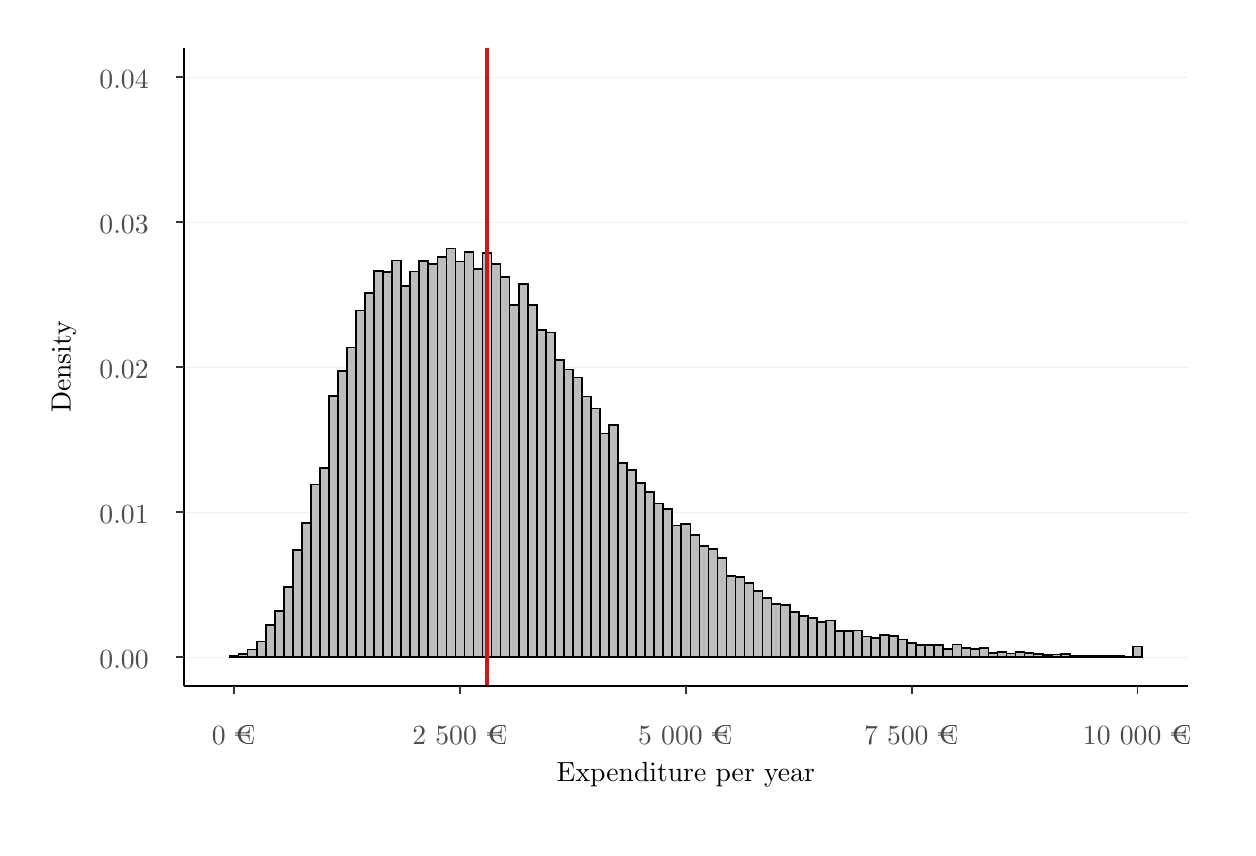
\begin{tikzpicture}[x=1pt,y=1pt]
\definecolor{fillColor}{RGB}{255,255,255}
\path[use as bounding box,fill=fillColor,fill opacity=0.00] (0,0) rectangle (433.62,289.08);
\begin{scope}
\path[clip] (  0.00,  0.00) rectangle (433.62,289.08);
\definecolor{drawColor}{RGB}{255,255,255}
\definecolor{fillColor}{RGB}{255,255,255}

\path[draw=drawColor,line width= 0.6pt,line join=round,line cap=round,fill=fillColor] ( -0.00,  0.00) rectangle (433.62,289.08);
\end{scope}
\begin{scope}
\path[clip] ( 56.47, 51.15) rectangle (419.17,281.85);
\definecolor{drawColor}{RGB}{255,255,255}

\path[draw=drawColor,line width= 0.3pt,line join=round] ( 56.47, 87.86) --
	(419.17, 87.86);

\path[draw=drawColor,line width= 0.3pt,line join=round] ( 56.47,140.29) --
	(419.17,140.29);

\path[draw=drawColor,line width= 0.3pt,line join=round] ( 56.47,192.72) --
	(419.17,192.72);

\path[draw=drawColor,line width= 0.3pt,line join=round] ( 56.47,245.15) --
	(419.17,245.15);

\path[draw=drawColor,line width= 0.3pt,line join=round] (115.39, 51.15) --
	(115.39,281.85);

\path[draw=drawColor,line width= 0.3pt,line join=round] (197.01, 51.15) --
	(197.01,281.85);

\path[draw=drawColor,line width= 0.3pt,line join=round] (278.62, 51.15) --
	(278.62,281.85);

\path[draw=drawColor,line width= 0.3pt,line join=round] (360.24, 51.15) --
	(360.24,281.85);
\definecolor{drawColor}{gray}{0.94}

\path[draw=drawColor,line width= 0.1pt,line join=round] ( 56.47, 61.64) --
	(419.17, 61.64);

\path[draw=drawColor,line width= 0.1pt,line join=round] ( 56.47,114.07) --
	(419.17,114.07);

\path[draw=drawColor,line width= 0.1pt,line join=round] ( 56.47,166.50) --
	(419.17,166.50);

\path[draw=drawColor,line width= 0.1pt,line join=round] ( 56.47,218.93) --
	(419.17,218.93);

\path[draw=drawColor,line width= 0.1pt,line join=round] ( 56.47,271.37) --
	(419.17,271.37);
\definecolor{drawColor}{RGB}{0,0,0}
\definecolor{fillColor}{gray}{0.74}

\path[draw=drawColor,line width= 0.6pt,line cap=rect,fill=fillColor] ( 72.95, 61.64) rectangle ( 76.22, 61.95);

\path[draw=drawColor,line width= 0.6pt,line cap=rect,fill=fillColor] ( 76.22, 61.64) rectangle ( 79.48, 62.75);

\path[draw=drawColor,line width= 0.6pt,line cap=rect,fill=fillColor] ( 79.48, 61.64) rectangle ( 82.75, 64.36);

\path[draw=drawColor,line width= 0.6pt,line cap=rect,fill=fillColor] ( 82.75, 61.64) rectangle ( 86.01, 67.27);

\path[draw=drawColor,line width= 0.6pt,line cap=rect,fill=fillColor] ( 86.01, 61.64) rectangle ( 89.28, 73.16);

\path[draw=drawColor,line width= 0.6pt,line cap=rect,fill=fillColor] ( 89.28, 61.64) rectangle ( 92.54, 78.36);

\path[draw=drawColor,line width= 0.6pt,line cap=rect,fill=fillColor] ( 92.54, 61.64) rectangle ( 95.80, 87.03);

\path[draw=drawColor,line width= 0.6pt,line cap=rect,fill=fillColor] ( 95.80, 61.64) rectangle ( 99.07,100.28);

\path[draw=drawColor,line width= 0.6pt,line cap=rect,fill=fillColor] ( 99.07, 61.64) rectangle (102.33,110.06);

\path[draw=drawColor,line width= 0.6pt,line cap=rect,fill=fillColor] (102.33, 61.64) rectangle (105.60,123.99);

\path[draw=drawColor,line width= 0.6pt,line cap=rect,fill=fillColor] (105.60, 61.64) rectangle (108.86,130.00);

\path[draw=drawColor,line width= 0.6pt,line cap=rect,fill=fillColor] (108.86, 61.64) rectangle (112.13,156.07);

\path[draw=drawColor,line width= 0.6pt,line cap=rect,fill=fillColor] (112.13, 61.64) rectangle (115.39,165.04);

\path[draw=drawColor,line width= 0.6pt,line cap=rect,fill=fillColor] (115.39, 61.64) rectangle (118.66,173.47);

\path[draw=drawColor,line width= 0.6pt,line cap=rect,fill=fillColor] (118.66, 61.64) rectangle (121.92,186.90);

\path[draw=drawColor,line width= 0.6pt,line cap=rect,fill=fillColor] (121.92, 61.64) rectangle (125.19,193.28);

\path[draw=drawColor,line width= 0.6pt,line cap=rect,fill=fillColor] (125.19, 61.64) rectangle (128.45,201.08);

\path[draw=drawColor,line width= 0.6pt,line cap=rect,fill=fillColor] (128.45, 61.64) rectangle (131.72,200.71);

\path[draw=drawColor,line width= 0.6pt,line cap=rect,fill=fillColor] (131.72, 61.64) rectangle (134.98,204.92);

\path[draw=drawColor,line width= 0.6pt,line cap=rect,fill=fillColor] (134.98, 61.64) rectangle (138.24,195.69);

\path[draw=drawColor,line width= 0.6pt,line cap=rect,fill=fillColor] (138.24, 61.64) rectangle (141.51,201.02);

\path[draw=drawColor,line width= 0.6pt,line cap=rect,fill=fillColor] (141.51, 61.64) rectangle (144.77,204.86);

\path[draw=drawColor,line width= 0.6pt,line cap=rect,fill=fillColor] (144.77, 61.64) rectangle (148.04,203.62);

\path[draw=drawColor,line width= 0.6pt,line cap=rect,fill=fillColor] (148.04, 61.64) rectangle (151.30,206.22);

\path[draw=drawColor,line width= 0.6pt,line cap=rect,fill=fillColor] (151.30, 61.64) rectangle (154.57,209.25);

\path[draw=drawColor,line width= 0.6pt,line cap=rect,fill=fillColor] (154.57, 61.64) rectangle (157.83,204.55);

\path[draw=drawColor,line width= 0.6pt,line cap=rect,fill=fillColor] (157.83, 61.64) rectangle (161.10,208.08);

\path[draw=drawColor,line width= 0.6pt,line cap=rect,fill=fillColor] (161.10, 61.64) rectangle (164.36,201.82);

\path[draw=drawColor,line width= 0.6pt,line cap=rect,fill=fillColor] (164.36, 61.64) rectangle (167.63,207.58);

\path[draw=drawColor,line width= 0.6pt,line cap=rect,fill=fillColor] (167.63, 61.64) rectangle (170.89,203.74);

\path[draw=drawColor,line width= 0.6pt,line cap=rect,fill=fillColor] (170.89, 61.64) rectangle (174.16,198.98);

\path[draw=drawColor,line width= 0.6pt,line cap=rect,fill=fillColor] (174.16, 61.64) rectangle (177.42,188.95);

\path[draw=drawColor,line width= 0.6pt,line cap=rect,fill=fillColor] (177.42, 61.64) rectangle (180.68,196.38);

\path[draw=drawColor,line width= 0.6pt,line cap=rect,fill=fillColor] (180.68, 61.64) rectangle (183.95,188.95);

\path[draw=drawColor,line width= 0.6pt,line cap=rect,fill=fillColor] (183.95, 61.64) rectangle (187.21,179.78);

\path[draw=drawColor,line width= 0.6pt,line cap=rect,fill=fillColor] (187.21, 61.64) rectangle (190.48,178.98);

\path[draw=drawColor,line width= 0.6pt,line cap=rect,fill=fillColor] (190.48, 61.64) rectangle (193.74,169.07);

\path[draw=drawColor,line width= 0.6pt,line cap=rect,fill=fillColor] (193.74, 61.64) rectangle (197.01,165.60);

\path[draw=drawColor,line width= 0.6pt,line cap=rect,fill=fillColor] (197.01, 61.64) rectangle (200.27,162.69);

\path[draw=drawColor,line width= 0.6pt,line cap=rect,fill=fillColor] (200.27, 61.64) rectangle (203.54,155.82);

\path[draw=drawColor,line width= 0.6pt,line cap=rect,fill=fillColor] (203.54, 61.64) rectangle (206.80,151.48);

\path[draw=drawColor,line width= 0.6pt,line cap=rect,fill=fillColor] (206.80, 61.64) rectangle (210.07,142.38);

\path[draw=drawColor,line width= 0.6pt,line cap=rect,fill=fillColor] (210.07, 61.64) rectangle (213.33,145.60);

\path[draw=drawColor,line width= 0.6pt,line cap=rect,fill=fillColor] (213.33, 61.64) rectangle (216.60,131.86);

\path[draw=drawColor,line width= 0.6pt,line cap=rect,fill=fillColor] (216.60, 61.64) rectangle (219.86,129.19);

\path[draw=drawColor,line width= 0.6pt,line cap=rect,fill=fillColor] (219.86, 61.64) rectangle (223.13,124.43);

\path[draw=drawColor,line width= 0.6pt,line cap=rect,fill=fillColor] (223.13, 61.64) rectangle (226.39,121.27);

\path[draw=drawColor,line width= 0.6pt,line cap=rect,fill=fillColor] (226.39, 61.64) rectangle (229.65,117.12);

\path[draw=drawColor,line width= 0.6pt,line cap=rect,fill=fillColor] (229.65, 61.64) rectangle (232.92,115.14);

\path[draw=drawColor,line width= 0.6pt,line cap=rect,fill=fillColor] (232.92, 61.64) rectangle (236.18,109.19);

\path[draw=drawColor,line width= 0.6pt,line cap=rect,fill=fillColor] (236.18, 61.64) rectangle (239.45,109.63);

\path[draw=drawColor,line width= 0.6pt,line cap=rect,fill=fillColor] (239.45, 61.64) rectangle (242.71,105.79);

\path[draw=drawColor,line width= 0.6pt,line cap=rect,fill=fillColor] (242.71, 61.64) rectangle (245.98,101.76);

\path[draw=drawColor,line width= 0.6pt,line cap=rect,fill=fillColor] (245.98, 61.64) rectangle (249.24,100.59);

\path[draw=drawColor,line width= 0.6pt,line cap=rect,fill=fillColor] (249.24, 61.64) rectangle (252.51, 97.49);

\path[draw=drawColor,line width= 0.6pt,line cap=rect,fill=fillColor] (252.51, 61.64) rectangle (255.77, 90.93);

\path[draw=drawColor,line width= 0.6pt,line cap=rect,fill=fillColor] (255.77, 61.64) rectangle (259.04, 90.49);

\path[draw=drawColor,line width= 0.6pt,line cap=rect,fill=fillColor] (259.04, 61.64) rectangle (262.30, 88.33);

\path[draw=drawColor,line width= 0.6pt,line cap=rect,fill=fillColor] (262.30, 61.64) rectangle (265.57, 85.54);

\path[draw=drawColor,line width= 0.6pt,line cap=rect,fill=fillColor] (265.57, 61.64) rectangle (268.83, 83.00);

\path[draw=drawColor,line width= 0.6pt,line cap=rect,fill=fillColor] (268.83, 61.64) rectangle (272.09, 80.71);

\path[draw=drawColor,line width= 0.6pt,line cap=rect,fill=fillColor] (272.09, 61.64) rectangle (275.36, 80.46);

\path[draw=drawColor,line width= 0.6pt,line cap=rect,fill=fillColor] (275.36, 61.64) rectangle (278.62, 77.86);

\path[draw=drawColor,line width= 0.6pt,line cap=rect,fill=fillColor] (278.62, 61.64) rectangle (281.89, 76.56);

\path[draw=drawColor,line width= 0.6pt,line cap=rect,fill=fillColor] (281.89, 61.64) rectangle (285.15, 75.82);

\path[draw=drawColor,line width= 0.6pt,line cap=rect,fill=fillColor] (285.15, 61.64) rectangle (288.42, 74.33);

\path[draw=drawColor,line width= 0.6pt,line cap=rect,fill=fillColor] (288.42, 61.64) rectangle (291.68, 74.83);

\path[draw=drawColor,line width= 0.6pt,line cap=rect,fill=fillColor] (291.68, 61.64) rectangle (294.95, 71.18);

\path[draw=drawColor,line width= 0.6pt,line cap=rect,fill=fillColor] (294.95, 61.64) rectangle (298.21, 71.18);

\path[draw=drawColor,line width= 0.6pt,line cap=rect,fill=fillColor] (298.21, 61.64) rectangle (301.48, 71.30);

\path[draw=drawColor,line width= 0.6pt,line cap=rect,fill=fillColor] (301.48, 61.64) rectangle (304.74, 69.07);

\path[draw=drawColor,line width= 0.6pt,line cap=rect,fill=fillColor] (304.74, 61.64) rectangle (308.01, 68.57);

\path[draw=drawColor,line width= 0.6pt,line cap=rect,fill=fillColor] (308.01, 61.64) rectangle (311.27, 69.69);

\path[draw=drawColor,line width= 0.6pt,line cap=rect,fill=fillColor] (311.27, 61.64) rectangle (314.53, 69.26);

\path[draw=drawColor,line width= 0.6pt,line cap=rect,fill=fillColor] (314.53, 61.64) rectangle (317.80, 67.96);

\path[draw=drawColor,line width= 0.6pt,line cap=rect,fill=fillColor] (317.80, 61.64) rectangle (321.06, 66.78);

\path[draw=drawColor,line width= 0.6pt,line cap=rect,fill=fillColor] (321.06, 61.64) rectangle (324.33, 65.97);

\path[draw=drawColor,line width= 0.6pt,line cap=rect,fill=fillColor] (324.33, 61.64) rectangle (327.59, 65.91);

\path[draw=drawColor,line width= 0.6pt,line cap=rect,fill=fillColor] (327.59, 61.64) rectangle (330.86, 65.91);

\path[draw=drawColor,line width= 0.6pt,line cap=rect,fill=fillColor] (330.86, 61.64) rectangle (334.12, 64.67);

\path[draw=drawColor,line width= 0.6pt,line cap=rect,fill=fillColor] (334.12, 61.64) rectangle (337.39, 66.16);

\path[draw=drawColor,line width= 0.6pt,line cap=rect,fill=fillColor] (337.39, 61.64) rectangle (340.65, 64.92);

\path[draw=drawColor,line width= 0.6pt,line cap=rect,fill=fillColor] (340.65, 61.64) rectangle (343.92, 64.61);

\path[draw=drawColor,line width= 0.6pt,line cap=rect,fill=fillColor] (343.92, 61.64) rectangle (347.18, 64.92);

\path[draw=drawColor,line width= 0.6pt,line cap=rect,fill=fillColor] (347.18, 61.64) rectangle (350.45, 63.13);

\path[draw=drawColor,line width= 0.6pt,line cap=rect,fill=fillColor] (350.45, 61.64) rectangle (353.71, 63.56);

\path[draw=drawColor,line width= 0.6pt,line cap=rect,fill=fillColor] (353.71, 61.64) rectangle (356.97, 62.88);

\path[draw=drawColor,line width= 0.6pt,line cap=rect,fill=fillColor] (356.97, 61.64) rectangle (360.24, 63.50);

\path[draw=drawColor,line width= 0.6pt,line cap=rect,fill=fillColor] (360.24, 61.64) rectangle (363.50, 63.13);

\path[draw=drawColor,line width= 0.6pt,line cap=rect,fill=fillColor] (363.50, 61.64) rectangle (366.77, 62.82);

\path[draw=drawColor,line width= 0.6pt,line cap=rect,fill=fillColor] (366.77, 61.64) rectangle (370.03, 62.38);

\path[draw=drawColor,line width= 0.6pt,line cap=rect,fill=fillColor] (370.03, 61.64) rectangle (373.30, 62.63);

\path[draw=drawColor,line width= 0.6pt,line cap=rect,fill=fillColor] (373.30, 61.64) rectangle (376.56, 62.69);

\path[draw=drawColor,line width= 0.6pt,line cap=rect,fill=fillColor] (376.56, 61.64) rectangle (379.83, 62.26);

\path[draw=drawColor,line width= 0.6pt,line cap=rect,fill=fillColor] (379.83, 61.64) rectangle (383.09, 62.07);

\path[draw=drawColor,line width= 0.6pt,line cap=rect,fill=fillColor] (383.09, 61.64) rectangle (386.36, 62.14);

\path[draw=drawColor,line width= 0.6pt,line cap=rect,fill=fillColor] (386.36, 61.64) rectangle (389.62, 62.20);

\path[draw=drawColor,line width= 0.6pt,line cap=rect,fill=fillColor] (389.62, 61.64) rectangle (392.89, 62.01);

\path[draw=drawColor,line width= 0.6pt,line cap=rect,fill=fillColor] (392.89, 61.64) rectangle (396.15, 62.01);

\path[draw=drawColor,line width= 0.6pt,line cap=rect,fill=fillColor] (396.15, 61.64) rectangle (399.41, 61.76);

\path[draw=drawColor,line width= 0.6pt,line cap=rect,fill=fillColor] (399.41, 61.64) rectangle (402.68, 65.48);
\definecolor{drawColor}{RGB}{203,24,29}

\path[draw=drawColor,line width= 1.7pt,line join=round] (166.01, 51.15) -- (166.01,281.85);
\end{scope}
\begin{scope}
\path[clip] (  0.00,  0.00) rectangle (433.62,289.08);
\definecolor{drawColor}{RGB}{0,0,0}

\path[draw=drawColor,line width= 0.6pt,line join=round] ( 56.47, 51.15) --
	( 56.47,281.85);
\end{scope}
\begin{scope}
\path[clip] (  0.00,  0.00) rectangle (433.62,289.08);
\definecolor{drawColor}{gray}{0.30}

\node[text=drawColor,anchor=base east,inner sep=0pt, outer sep=0pt, scale=  1.00] at ( 43.72, 57.51) {0.00};

\node[text=drawColor,anchor=base east,inner sep=0pt, outer sep=0pt, scale=  1.00] at ( 43.72,109.94) {0.01};

\node[text=drawColor,anchor=base east,inner sep=0pt, outer sep=0pt, scale=  1.00] at ( 43.72,162.37) {0.02};

\node[text=drawColor,anchor=base east,inner sep=0pt, outer sep=0pt, scale=  1.00] at ( 43.72,214.80) {0.03};

\node[text=drawColor,anchor=base east,inner sep=0pt, outer sep=0pt, scale=  1.00] at ( 43.72,267.23) {0.04};
\end{scope}
\begin{scope}
\path[clip] (  0.00,  0.00) rectangle (433.62,289.08);
\definecolor{drawColor}{gray}{0.20}

\path[draw=drawColor,line width= 0.6pt,line join=round] ( 53.72, 61.64) --
	( 56.47, 61.64);

\path[draw=drawColor,line width= 0.6pt,line join=round] ( 53.72,114.07) --
	( 56.47,114.07);

\path[draw=drawColor,line width= 0.6pt,line join=round] ( 53.72,166.50) --
	( 56.47,166.50);

\path[draw=drawColor,line width= 0.6pt,line join=round] ( 53.72,218.93) --
	( 56.47,218.93);

\path[draw=drawColor,line width= 0.6pt,line join=round] ( 53.72,271.37) --
	( 56.47,271.37);
\end{scope}
\begin{scope}
\path[clip] (  0.00,  0.00) rectangle (433.62,289.08);
\definecolor{drawColor}{RGB}{0,0,0}

\path[draw=drawColor,line width= 0.6pt,line join=round] ( 56.47, 51.15) --
	(419.17, 51.15);
\end{scope}
\begin{scope}
\path[clip] (  0.00,  0.00) rectangle (433.62,289.08);
\definecolor{drawColor}{gray}{0.20}

\path[draw=drawColor,line width= 0.6pt,line join=round] ( 74.58, 48.40) --
	( 74.58, 51.15);

\path[draw=drawColor,line width= 0.6pt,line join=round] (156.20, 48.40) --
	(156.20, 51.15);

\path[draw=drawColor,line width= 0.6pt,line join=round] (237.82, 48.40) --
	(237.82, 51.15);

\path[draw=drawColor,line width= 0.6pt,line join=round] (319.43, 48.40) --
	(319.43, 51.15);

\path[draw=drawColor,line width= 0.6pt,line join=round] (401.05, 48.40) --
	(401.05, 51.15);
\end{scope}
\begin{scope}
\path[clip] (  0.00,  0.00) rectangle (433.62,289.08);
\definecolor{drawColor}{gray}{0.30}

\node[text=drawColor,anchor=base,inner sep=0pt, outer sep=0pt, scale=  1.00] at ( 74.58, 30.14) {0 €};

\node[text=drawColor,anchor=base,inner sep=0pt, outer sep=0pt, scale=  1.00] at (156.20, 30.14) {2 500 €};

\node[text=drawColor,anchor=base,inner sep=0pt, outer sep=0pt, scale=  1.00] at (237.82, 30.14) {5 000 €};

\node[text=drawColor,anchor=base,inner sep=0pt, outer sep=0pt, scale=  1.00] at (319.43, 30.14) {7 500 €};

\node[text=drawColor,anchor=base,inner sep=0pt, outer sep=0pt, scale=  1.00] at (401.05, 30.14) {10 000 €};
\end{scope}
\begin{scope}
\path[clip] (  0.00,  0.00) rectangle (433.62,289.08);
\definecolor{drawColor}{RGB}{0,0,0}

\node[text=drawColor,anchor=base,inner sep=0pt, outer sep=0pt, scale=  1.00] at (237.82, 16.79) {Expenditure per year};
\end{scope}
\begin{scope}
\path[clip] (  0.00,  0.00) rectangle (433.62,289.08);
\definecolor{drawColor}{RGB}{0,0,0}

\node[text=drawColor,rotate= 90.00,anchor=base,inner sep=0pt, outer sep=0pt, scale=  1.00] at ( 15.49,166.50) {Density};
\end{scope}
\end{tikzpicture}
}
    \end{subfigure}
    \parbox{\textwidth}{
        \begin{spacing}{1} 
            {\footnotesize 
            \textit{Notes}: These figures plot the distribution of average expenditure per year across households in the final sample on the 68 included product categories for each country.}
        \end{spacing}}
\end{figure} 

\begin{figure}[H]
    \centering
    \caption{Barcodes per year}
    \label{fig: app_data_households_bar_year}
    \begin{subfigure}[t]{.49\textwidth}
         \centering
         \caption{Belgium}
         \scalebox{0.45}{% Created by tikzDevice version 0.12.3.1 on 2022-07-29 15:13:36
% !TEX encoding = UTF-8 Unicode
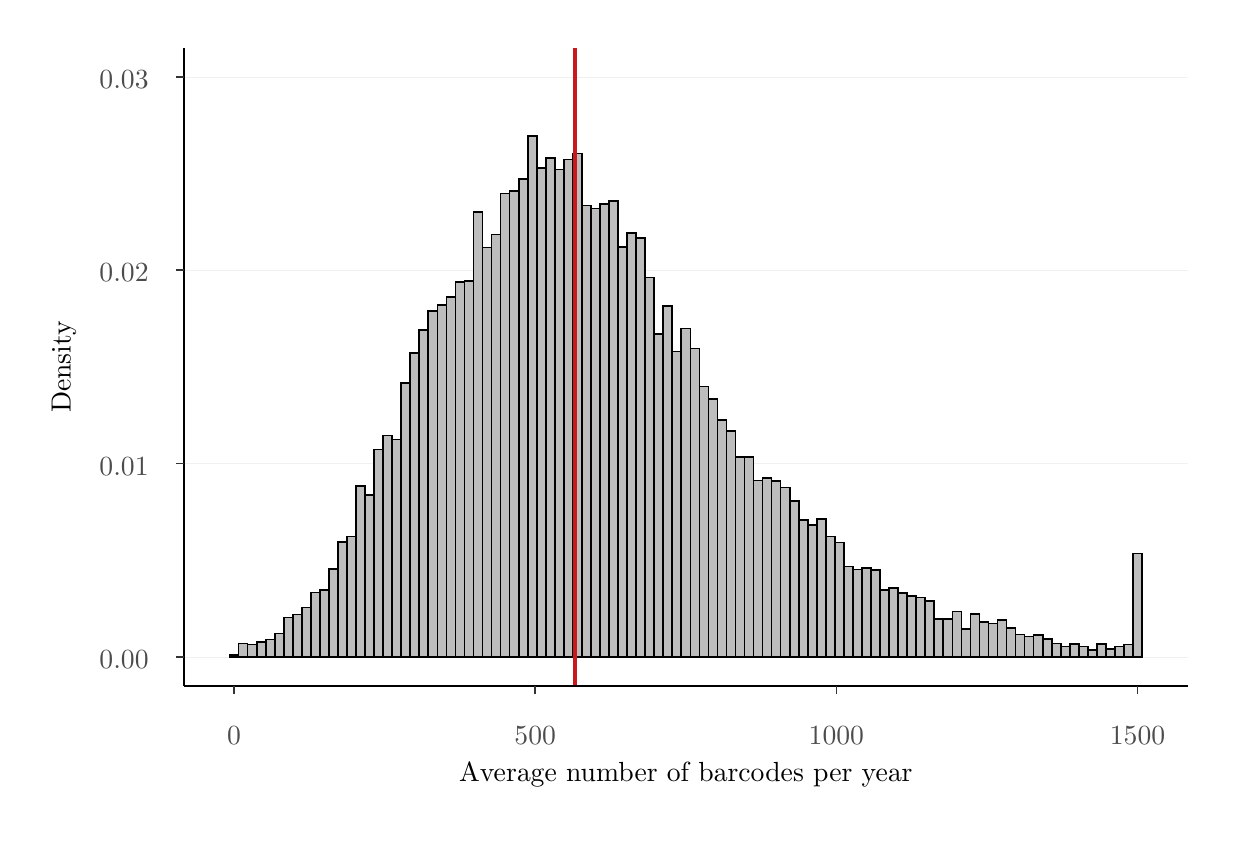
\begin{tikzpicture}[x=1pt,y=1pt]
\definecolor{fillColor}{RGB}{255,255,255}
\path[use as bounding box,fill=fillColor,fill opacity=0.00] (0,0) rectangle (433.62,289.08);
\begin{scope}
\path[clip] (  0.00,  0.00) rectangle (433.62,289.08);
\definecolor{drawColor}{RGB}{255,255,255}
\definecolor{fillColor}{RGB}{255,255,255}

\path[draw=drawColor,line width= 0.6pt,line join=round,line cap=round,fill=fillColor] ( -0.00,  0.00) rectangle (433.62,289.08);
\end{scope}
\begin{scope}
\path[clip] ( 56.47, 51.15) rectangle (419.17,281.85);
\definecolor{drawColor}{RGB}{255,255,255}

\path[draw=drawColor,line width= 0.3pt,line join=round] ( 56.47, 96.59) --
	(419.17, 96.59);

\path[draw=drawColor,line width= 0.3pt,line join=round] ( 56.47,166.50) --
	(419.17,166.50);

\path[draw=drawColor,line width= 0.3pt,line join=round] ( 56.47,236.41) --
	(419.17,236.41);

\path[draw=drawColor,line width= 0.3pt,line join=round] (128.99, 51.15) --
	(128.99,281.85);

\path[draw=drawColor,line width= 0.3pt,line join=round] (237.82, 51.15) --
	(237.82,281.85);

\path[draw=drawColor,line width= 0.3pt,line join=round] (346.64, 51.15) --
	(346.64,281.85);
\definecolor{drawColor}{gray}{0.94}

\path[draw=drawColor,line width= 0.1pt,line join=round] ( 56.47, 61.64) --
	(419.17, 61.64);

\path[draw=drawColor,line width= 0.1pt,line join=round] ( 56.47,131.55) --
	(419.17,131.55);

\path[draw=drawColor,line width= 0.1pt,line join=round] ( 56.47,201.46) --
	(419.17,201.46);

\path[draw=drawColor,line width= 0.1pt,line join=round] ( 56.47,271.37) --
	(419.17,271.37);
\definecolor{drawColor}{RGB}{0,0,0}
\definecolor{fillColor}{gray}{0.74}

\path[draw=drawColor,line width= 0.6pt,line cap=rect,fill=fillColor] ( 72.95, 61.64) rectangle ( 76.22, 62.49);

\path[draw=drawColor,line width= 0.6pt,line cap=rect,fill=fillColor] ( 76.22, 61.64) rectangle ( 79.48, 66.55);

\path[draw=drawColor,line width= 0.6pt,line cap=rect,fill=fillColor] ( 79.48, 61.64) rectangle ( 82.75, 66.13);

\path[draw=drawColor,line width= 0.6pt,line cap=rect,fill=fillColor] ( 82.75, 61.64) rectangle ( 86.01, 66.98);

\path[draw=drawColor,line width= 0.6pt,line cap=rect,fill=fillColor] ( 86.01, 61.64) rectangle ( 89.28, 68.05);

\path[draw=drawColor,line width= 0.6pt,line cap=rect,fill=fillColor] ( 89.28, 61.64) rectangle ( 92.54, 70.18);

\path[draw=drawColor,line width= 0.6pt,line cap=rect,fill=fillColor] ( 92.54, 61.64) rectangle ( 95.80, 75.95);

\path[draw=drawColor,line width= 0.6pt,line cap=rect,fill=fillColor] ( 95.80, 61.64) rectangle ( 99.07, 77.02);

\path[draw=drawColor,line width= 0.6pt,line cap=rect,fill=fillColor] ( 99.07, 61.64) rectangle (102.33, 79.58);

\path[draw=drawColor,line width= 0.6pt,line cap=rect,fill=fillColor] (102.33, 61.64) rectangle (105.60, 84.92);

\path[draw=drawColor,line width= 0.6pt,line cap=rect,fill=fillColor] (105.60, 61.64) rectangle (108.86, 85.78);

\path[draw=drawColor,line width= 0.6pt,line cap=rect,fill=fillColor] (108.86, 61.64) rectangle (112.13, 93.47);

\path[draw=drawColor,line width= 0.6pt,line cap=rect,fill=fillColor] (112.13, 61.64) rectangle (115.39,103.29);

\path[draw=drawColor,line width= 0.6pt,line cap=rect,fill=fillColor] (115.39, 61.64) rectangle (118.66,105.21);

\path[draw=drawColor,line width= 0.6pt,line cap=rect,fill=fillColor] (118.66, 61.64) rectangle (121.92,123.37);

\path[draw=drawColor,line width= 0.6pt,line cap=rect,fill=fillColor] (121.92, 61.64) rectangle (125.19,120.17);

\path[draw=drawColor,line width= 0.6pt,line cap=rect,fill=fillColor] (125.19, 61.64) rectangle (128.45,136.61);

\path[draw=drawColor,line width= 0.6pt,line cap=rect,fill=fillColor] (128.45, 61.64) rectangle (131.72,141.74);

\path[draw=drawColor,line width= 0.6pt,line cap=rect,fill=fillColor] (131.72, 61.64) rectangle (134.98,140.24);

\path[draw=drawColor,line width= 0.6pt,line cap=rect,fill=fillColor] (134.98, 61.64) rectangle (138.24,160.75);

\path[draw=drawColor,line width= 0.6pt,line cap=rect,fill=fillColor] (138.24, 61.64) rectangle (141.51,171.43);

\path[draw=drawColor,line width= 0.6pt,line cap=rect,fill=fillColor] (141.51, 61.64) rectangle (144.77,179.76);

\path[draw=drawColor,line width= 0.6pt,line cap=rect,fill=fillColor] (144.77, 61.64) rectangle (148.04,186.81);

\path[draw=drawColor,line width= 0.6pt,line cap=rect,fill=fillColor] (148.04, 61.64) rectangle (151.30,188.95);

\path[draw=drawColor,line width= 0.6pt,line cap=rect,fill=fillColor] (151.30, 61.64) rectangle (154.57,191.72);

\path[draw=drawColor,line width= 0.6pt,line cap=rect,fill=fillColor] (154.57, 61.64) rectangle (157.83,197.28);

\path[draw=drawColor,line width= 0.6pt,line cap=rect,fill=fillColor] (157.83, 61.64) rectangle (161.10,197.49);

\path[draw=drawColor,line width= 0.6pt,line cap=rect,fill=fillColor] (161.10, 61.64) rectangle (164.36,222.48);

\path[draw=drawColor,line width= 0.6pt,line cap=rect,fill=fillColor] (164.36, 61.64) rectangle (167.63,209.66);

\path[draw=drawColor,line width= 0.6pt,line cap=rect,fill=fillColor] (167.63, 61.64) rectangle (170.89,214.36);

\path[draw=drawColor,line width= 0.6pt,line cap=rect,fill=fillColor] (170.89, 61.64) rectangle (174.16,229.10);

\path[draw=drawColor,line width= 0.6pt,line cap=rect,fill=fillColor] (174.16, 61.64) rectangle (177.42,229.96);

\path[draw=drawColor,line width= 0.6pt,line cap=rect,fill=fillColor] (177.42, 61.64) rectangle (180.68,234.44);

\path[draw=drawColor,line width= 0.6pt,line cap=rect,fill=fillColor] (180.68, 61.64) rectangle (183.95,249.82);

\path[draw=drawColor,line width= 0.6pt,line cap=rect,fill=fillColor] (183.95, 61.64) rectangle (187.21,238.29);

\path[draw=drawColor,line width= 0.6pt,line cap=rect,fill=fillColor] (187.21, 61.64) rectangle (190.48,241.92);

\path[draw=drawColor,line width= 0.6pt,line cap=rect,fill=fillColor] (190.48, 61.64) rectangle (193.74,237.86);

\path[draw=drawColor,line width= 0.6pt,line cap=rect,fill=fillColor] (193.74, 61.64) rectangle (197.01,241.49);

\path[draw=drawColor,line width= 0.6pt,line cap=rect,fill=fillColor] (197.01, 61.64) rectangle (200.27,243.63);

\path[draw=drawColor,line width= 0.6pt,line cap=rect,fill=fillColor] (200.27, 61.64) rectangle (203.54,224.83);

\path[draw=drawColor,line width= 0.6pt,line cap=rect,fill=fillColor] (203.54, 61.64) rectangle (206.80,223.76);

\path[draw=drawColor,line width= 0.6pt,line cap=rect,fill=fillColor] (206.80, 61.64) rectangle (210.07,225.47);

\path[draw=drawColor,line width= 0.6pt,line cap=rect,fill=fillColor] (210.07, 61.64) rectangle (213.33,226.54);

\path[draw=drawColor,line width= 0.6pt,line cap=rect,fill=fillColor] (213.33, 61.64) rectangle (216.60,209.88);

\path[draw=drawColor,line width= 0.6pt,line cap=rect,fill=fillColor] (216.60, 61.64) rectangle (219.86,215.00);

\path[draw=drawColor,line width= 0.6pt,line cap=rect,fill=fillColor] (219.86, 61.64) rectangle (223.13,213.08);

\path[draw=drawColor,line width= 0.6pt,line cap=rect,fill=fillColor] (223.13, 61.64) rectangle (226.39,198.77);

\path[draw=drawColor,line width= 0.6pt,line cap=rect,fill=fillColor] (226.39, 61.64) rectangle (229.65,178.48);

\path[draw=drawColor,line width= 0.6pt,line cap=rect,fill=fillColor] (229.65, 61.64) rectangle (232.92,188.52);

\path[draw=drawColor,line width= 0.6pt,line cap=rect,fill=fillColor] (232.92, 61.64) rectangle (236.18,172.07);

\path[draw=drawColor,line width= 0.6pt,line cap=rect,fill=fillColor] (236.18, 61.64) rectangle (239.45,180.40);

\path[draw=drawColor,line width= 0.6pt,line cap=rect,fill=fillColor] (239.45, 61.64) rectangle (242.71,173.14);

\path[draw=drawColor,line width= 0.6pt,line cap=rect,fill=fillColor] (242.71, 61.64) rectangle (245.98,159.47);

\path[draw=drawColor,line width= 0.6pt,line cap=rect,fill=fillColor] (245.98, 61.64) rectangle (249.24,154.98);

\path[draw=drawColor,line width= 0.6pt,line cap=rect,fill=fillColor] (249.24, 61.64) rectangle (252.51,147.29);

\path[draw=drawColor,line width= 0.6pt,line cap=rect,fill=fillColor] (252.51, 61.64) rectangle (255.77,143.45);

\path[draw=drawColor,line width= 0.6pt,line cap=rect,fill=fillColor] (255.77, 61.64) rectangle (259.04,133.84);

\path[draw=drawColor,line width= 0.6pt,line cap=rect,fill=fillColor] (259.04, 61.64) rectangle (262.30,134.05);

\path[draw=drawColor,line width= 0.6pt,line cap=rect,fill=fillColor] (262.30, 61.64) rectangle (265.57,125.51);

\path[draw=drawColor,line width= 0.6pt,line cap=rect,fill=fillColor] (265.57, 61.64) rectangle (268.83,126.36);

\path[draw=drawColor,line width= 0.6pt,line cap=rect,fill=fillColor] (268.83, 61.64) rectangle (272.09,125.29);

\path[draw=drawColor,line width= 0.6pt,line cap=rect,fill=fillColor] (272.09, 61.64) rectangle (275.36,122.94);

\path[draw=drawColor,line width= 0.6pt,line cap=rect,fill=fillColor] (275.36, 61.64) rectangle (278.62,118.03);

\path[draw=drawColor,line width= 0.6pt,line cap=rect,fill=fillColor] (278.62, 61.64) rectangle (281.89,111.19);

\path[draw=drawColor,line width= 0.6pt,line cap=rect,fill=fillColor] (281.89, 61.64) rectangle (285.15,109.27);

\path[draw=drawColor,line width= 0.6pt,line cap=rect,fill=fillColor] (285.15, 61.64) rectangle (288.42,111.62);

\path[draw=drawColor,line width= 0.6pt,line cap=rect,fill=fillColor] (288.42, 61.64) rectangle (291.68,105.21);

\path[draw=drawColor,line width= 0.6pt,line cap=rect,fill=fillColor] (291.68, 61.64) rectangle (294.95,103.08);

\path[draw=drawColor,line width= 0.6pt,line cap=rect,fill=fillColor] (294.95, 61.64) rectangle (298.21, 94.32);

\path[draw=drawColor,line width= 0.6pt,line cap=rect,fill=fillColor] (298.21, 61.64) rectangle (301.48, 93.25);

\path[draw=drawColor,line width= 0.6pt,line cap=rect,fill=fillColor] (301.48, 61.64) rectangle (304.74, 93.89);

\path[draw=drawColor,line width= 0.6pt,line cap=rect,fill=fillColor] (304.74, 61.64) rectangle (308.01, 93.04);

\path[draw=drawColor,line width= 0.6pt,line cap=rect,fill=fillColor] (308.01, 61.64) rectangle (311.27, 85.78);

\path[draw=drawColor,line width= 0.6pt,line cap=rect,fill=fillColor] (311.27, 61.64) rectangle (314.53, 86.63);

\path[draw=drawColor,line width= 0.6pt,line cap=rect,fill=fillColor] (314.53, 61.64) rectangle (317.80, 84.71);

\path[draw=drawColor,line width= 0.6pt,line cap=rect,fill=fillColor] (317.80, 61.64) rectangle (321.06, 83.64);

\path[draw=drawColor,line width= 0.6pt,line cap=rect,fill=fillColor] (321.06, 61.64) rectangle (324.33, 83.21);

\path[draw=drawColor,line width= 0.6pt,line cap=rect,fill=fillColor] (324.33, 61.64) rectangle (327.59, 81.93);

\path[draw=drawColor,line width= 0.6pt,line cap=rect,fill=fillColor] (327.59, 61.64) rectangle (330.86, 75.52);

\path[draw=drawColor,line width= 0.6pt,line cap=rect,fill=fillColor] (330.86, 61.64) rectangle (334.12, 75.52);

\path[draw=drawColor,line width= 0.6pt,line cap=rect,fill=fillColor] (334.12, 61.64) rectangle (337.39, 78.09);

\path[draw=drawColor,line width= 0.6pt,line cap=rect,fill=fillColor] (337.39, 61.64) rectangle (340.65, 71.68);

\path[draw=drawColor,line width= 0.6pt,line cap=rect,fill=fillColor] (340.65, 61.64) rectangle (343.92, 77.23);

\path[draw=drawColor,line width= 0.6pt,line cap=rect,fill=fillColor] (343.92, 61.64) rectangle (347.18, 74.24);

\path[draw=drawColor,line width= 0.6pt,line cap=rect,fill=fillColor] (347.18, 61.64) rectangle (350.45, 73.82);

\path[draw=drawColor,line width= 0.6pt,line cap=rect,fill=fillColor] (350.45, 61.64) rectangle (353.71, 75.10);

\path[draw=drawColor,line width= 0.6pt,line cap=rect,fill=fillColor] (353.71, 61.64) rectangle (356.97, 72.11);

\path[draw=drawColor,line width= 0.6pt,line cap=rect,fill=fillColor] (356.97, 61.64) rectangle (360.24, 69.76);

\path[draw=drawColor,line width= 0.6pt,line cap=rect,fill=fillColor] (360.24, 61.64) rectangle (363.50, 69.12);

\path[draw=drawColor,line width= 0.6pt,line cap=rect,fill=fillColor] (363.50, 61.64) rectangle (366.77, 69.54);

\path[draw=drawColor,line width= 0.6pt,line cap=rect,fill=fillColor] (366.77, 61.64) rectangle (370.03, 68.26);

\path[draw=drawColor,line width= 0.6pt,line cap=rect,fill=fillColor] (370.03, 61.64) rectangle (373.30, 66.55);

\path[draw=drawColor,line width= 0.6pt,line cap=rect,fill=fillColor] (373.30, 61.64) rectangle (376.56, 65.48);

\path[draw=drawColor,line width= 0.6pt,line cap=rect,fill=fillColor] (376.56, 61.64) rectangle (379.83, 66.34);

\path[draw=drawColor,line width= 0.6pt,line cap=rect,fill=fillColor] (379.83, 61.64) rectangle (383.09, 65.48);

\path[draw=drawColor,line width= 0.6pt,line cap=rect,fill=fillColor] (383.09, 61.64) rectangle (386.36, 64.20);

\path[draw=drawColor,line width= 0.6pt,line cap=rect,fill=fillColor] (386.36, 61.64) rectangle (389.62, 66.34);

\path[draw=drawColor,line width= 0.6pt,line cap=rect,fill=fillColor] (389.62, 61.64) rectangle (392.89, 64.63);

\path[draw=drawColor,line width= 0.6pt,line cap=rect,fill=fillColor] (392.89, 61.64) rectangle (396.15, 65.48);

\path[draw=drawColor,line width= 0.6pt,line cap=rect,fill=fillColor] (396.15, 61.64) rectangle (399.41, 66.13);

\path[draw=drawColor,line width= 0.6pt,line cap=rect,fill=fillColor] (399.41, 61.64) rectangle (402.68, 99.02);
\definecolor{drawColor}{RGB}{203,24,29}

\path[draw=drawColor,line width= 1.7pt,line join=round] (197.77, 51.15) -- (197.77,281.85);
\end{scope}
\begin{scope}
\path[clip] (  0.00,  0.00) rectangle (433.62,289.08);
\definecolor{drawColor}{RGB}{0,0,0}

\path[draw=drawColor,line width= 0.6pt,line join=round] ( 56.47, 51.15) --
	( 56.47,281.85);
\end{scope}
\begin{scope}
\path[clip] (  0.00,  0.00) rectangle (433.62,289.08);
\definecolor{drawColor}{gray}{0.30}

\node[text=drawColor,anchor=base east,inner sep=0pt, outer sep=0pt, scale=  1.00] at ( 43.72, 57.51) {0.00};

\node[text=drawColor,anchor=base east,inner sep=0pt, outer sep=0pt, scale=  1.00] at ( 43.72,127.42) {0.01};

\node[text=drawColor,anchor=base east,inner sep=0pt, outer sep=0pt, scale=  1.00] at ( 43.72,197.32) {0.02};

\node[text=drawColor,anchor=base east,inner sep=0pt, outer sep=0pt, scale=  1.00] at ( 43.72,267.23) {0.03};
\end{scope}
\begin{scope}
\path[clip] (  0.00,  0.00) rectangle (433.62,289.08);
\definecolor{drawColor}{gray}{0.20}

\path[draw=drawColor,line width= 0.6pt,line join=round] ( 53.72, 61.64) --
	( 56.47, 61.64);

\path[draw=drawColor,line width= 0.6pt,line join=round] ( 53.72,131.55) --
	( 56.47,131.55);

\path[draw=drawColor,line width= 0.6pt,line join=round] ( 53.72,201.46) --
	( 56.47,201.46);

\path[draw=drawColor,line width= 0.6pt,line join=round] ( 53.72,271.37) --
	( 56.47,271.37);
\end{scope}
\begin{scope}
\path[clip] (  0.00,  0.00) rectangle (433.62,289.08);
\definecolor{drawColor}{RGB}{0,0,0}

\path[draw=drawColor,line width= 0.6pt,line join=round] ( 56.47, 51.15) --
	(419.17, 51.15);
\end{scope}
\begin{scope}
\path[clip] (  0.00,  0.00) rectangle (433.62,289.08);
\definecolor{drawColor}{gray}{0.20}

\path[draw=drawColor,line width= 0.6pt,line join=round] ( 74.58, 48.40) --
	( 74.58, 51.15);

\path[draw=drawColor,line width= 0.6pt,line join=round] (183.41, 48.40) --
	(183.41, 51.15);

\path[draw=drawColor,line width= 0.6pt,line join=round] (292.23, 48.40) --
	(292.23, 51.15);

\path[draw=drawColor,line width= 0.6pt,line join=round] (401.05, 48.40) --
	(401.05, 51.15);
\end{scope}
\begin{scope}
\path[clip] (  0.00,  0.00) rectangle (433.62,289.08);
\definecolor{drawColor}{gray}{0.30}

\node[text=drawColor,anchor=base,inner sep=0pt, outer sep=0pt, scale=  1.00] at ( 74.58, 30.14) {0};

\node[text=drawColor,anchor=base,inner sep=0pt, outer sep=0pt, scale=  1.00] at (183.41, 30.14) {500};

\node[text=drawColor,anchor=base,inner sep=0pt, outer sep=0pt, scale=  1.00] at (292.23, 30.14) {1000};

\node[text=drawColor,anchor=base,inner sep=0pt, outer sep=0pt, scale=  1.00] at (401.05, 30.14) {1500};
\end{scope}
\begin{scope}
\path[clip] (  0.00,  0.00) rectangle (433.62,289.08);
\definecolor{drawColor}{RGB}{0,0,0}

\node[text=drawColor,anchor=base,inner sep=0pt, outer sep=0pt, scale=  1.00] at (237.82, 16.79) {Average number of barcodes per year};
\end{scope}
\begin{scope}
\path[clip] (  0.00,  0.00) rectangle (433.62,289.08);
\definecolor{drawColor}{RGB}{0,0,0}

\node[text=drawColor,rotate= 90.00,anchor=base,inner sep=0pt, outer sep=0pt, scale=  1.00] at ( 15.49,166.50) {Density};
\end{scope}
\end{tikzpicture}
}
     \end{subfigure}
     \begin{subfigure}[t]{.49\textwidth}
         \centering
         \caption{France}
         \scalebox{0.45}{% Created by tikzDevice version 0.12.3.1 on 2022-07-29 15:13:39
% !TEX encoding = UTF-8 Unicode
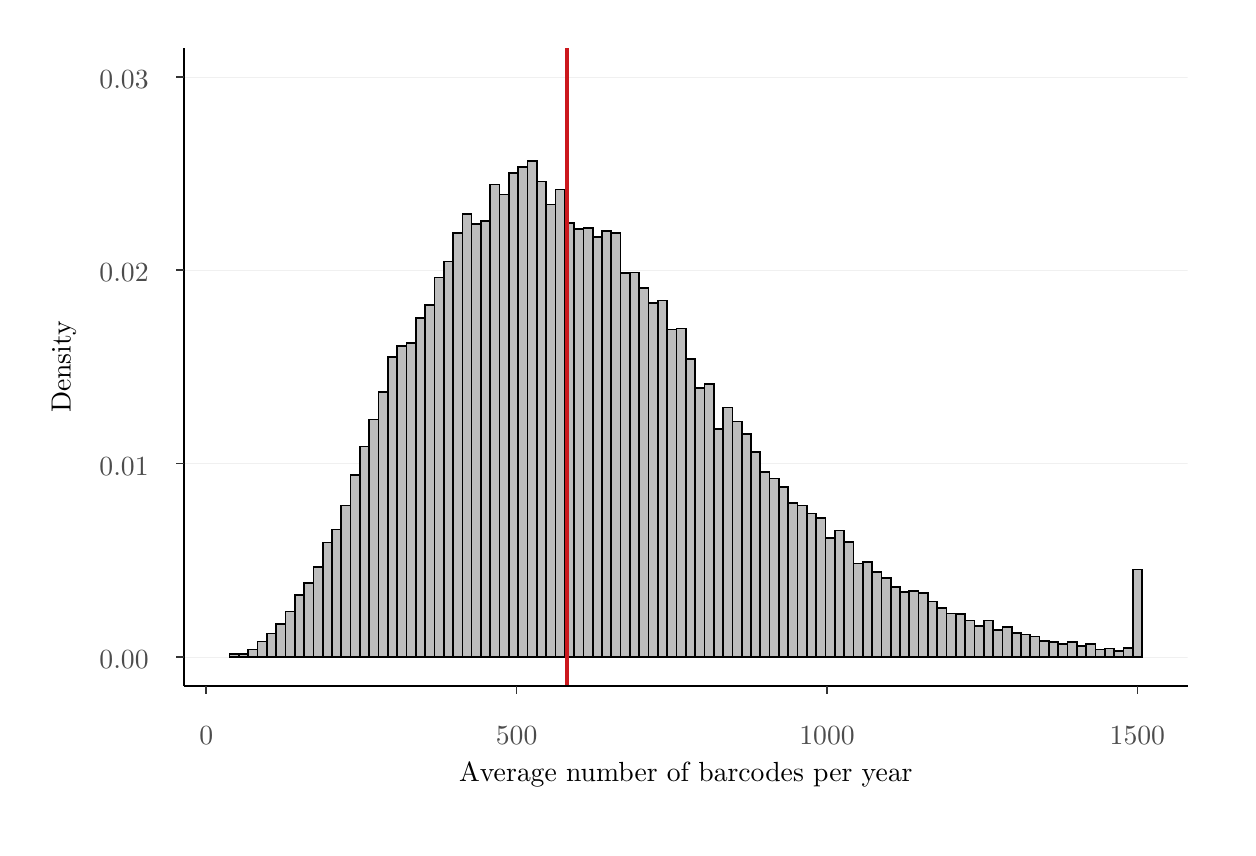
\begin{tikzpicture}[x=1pt,y=1pt]
\definecolor{fillColor}{RGB}{255,255,255}
\path[use as bounding box,fill=fillColor,fill opacity=0.00] (0,0) rectangle (433.62,289.08);
\begin{scope}
\path[clip] (  0.00,  0.00) rectangle (433.62,289.08);
\definecolor{drawColor}{RGB}{255,255,255}
\definecolor{fillColor}{RGB}{255,255,255}

\path[draw=drawColor,line width= 0.6pt,line join=round,line cap=round,fill=fillColor] ( -0.00,  0.00) rectangle (433.62,289.08);
\end{scope}
\begin{scope}
\path[clip] ( 56.47, 51.15) rectangle (419.17,281.85);
\definecolor{drawColor}{RGB}{255,255,255}

\path[draw=drawColor,line width= 0.3pt,line join=round] ( 56.47, 96.59) --
	(419.17, 96.59);

\path[draw=drawColor,line width= 0.3pt,line join=round] ( 56.47,166.50) --
	(419.17,166.50);

\path[draw=drawColor,line width= 0.3pt,line join=round] ( 56.47,236.41) --
	(419.17,236.41);

\path[draw=drawColor,line width= 0.3pt,line join=round] (120.62, 51.15) --
	(120.62,281.85);

\path[draw=drawColor,line width= 0.3pt,line join=round] (232.77, 51.15) --
	(232.77,281.85);

\path[draw=drawColor,line width= 0.3pt,line join=round] (344.92, 51.15) --
	(344.92,281.85);
\definecolor{drawColor}{gray}{0.94}

\path[draw=drawColor,line width= 0.1pt,line join=round] ( 56.47, 61.64) --
	(419.17, 61.64);

\path[draw=drawColor,line width= 0.1pt,line join=round] ( 56.47,131.55) --
	(419.17,131.55);

\path[draw=drawColor,line width= 0.1pt,line join=round] ( 56.47,201.46) --
	(419.17,201.46);

\path[draw=drawColor,line width= 0.1pt,line join=round] ( 56.47,271.37) --
	(419.17,271.37);
\definecolor{drawColor}{RGB}{0,0,0}
\definecolor{fillColor}{gray}{0.74}

\path[draw=drawColor,line width= 0.6pt,line cap=rect,fill=fillColor] ( 72.95, 61.64) rectangle ( 76.32, 62.74);

\path[draw=drawColor,line width= 0.6pt,line cap=rect,fill=fillColor] ( 76.32, 61.64) rectangle ( 79.68, 62.64);

\path[draw=drawColor,line width= 0.6pt,line cap=rect,fill=fillColor] ( 79.68, 61.64) rectangle ( 83.05, 64.33);

\path[draw=drawColor,line width= 0.6pt,line cap=rect,fill=fillColor] ( 83.05, 61.64) rectangle ( 86.41, 67.32);

\path[draw=drawColor,line width= 0.6pt,line cap=rect,fill=fillColor] ( 86.41, 61.64) rectangle ( 89.77, 70.11);

\path[draw=drawColor,line width= 0.6pt,line cap=rect,fill=fillColor] ( 89.77, 61.64) rectangle ( 93.14, 73.60);

\path[draw=drawColor,line width= 0.6pt,line cap=rect,fill=fillColor] ( 93.14, 61.64) rectangle ( 96.50, 78.08);

\path[draw=drawColor,line width= 0.6pt,line cap=rect,fill=fillColor] ( 96.50, 61.64) rectangle ( 99.87, 84.06);

\path[draw=drawColor,line width= 0.6pt,line cap=rect,fill=fillColor] ( 99.87, 61.64) rectangle (103.23, 88.45);

\path[draw=drawColor,line width= 0.6pt,line cap=rect,fill=fillColor] (103.23, 61.64) rectangle (106.60, 94.23);

\path[draw=drawColor,line width= 0.6pt,line cap=rect,fill=fillColor] (106.60, 61.64) rectangle (109.96,103.00);

\path[draw=drawColor,line width= 0.6pt,line cap=rect,fill=fillColor] (109.96, 61.64) rectangle (113.33,107.78);

\path[draw=drawColor,line width= 0.6pt,line cap=rect,fill=fillColor] (113.33, 61.64) rectangle (116.69,116.45);

\path[draw=drawColor,line width= 0.6pt,line cap=rect,fill=fillColor] (116.69, 61.64) rectangle (120.06,127.41);

\path[draw=drawColor,line width= 0.6pt,line cap=rect,fill=fillColor] (120.06, 61.64) rectangle (123.42,137.78);

\path[draw=drawColor,line width= 0.6pt,line cap=rect,fill=fillColor] (123.42, 61.64) rectangle (126.79,147.54);

\path[draw=drawColor,line width= 0.6pt,line cap=rect,fill=fillColor] (126.79, 61.64) rectangle (130.15,157.31);

\path[draw=drawColor,line width= 0.6pt,line cap=rect,fill=fillColor] (130.15, 61.64) rectangle (133.51,169.96);

\path[draw=drawColor,line width= 0.6pt,line cap=rect,fill=fillColor] (133.51, 61.64) rectangle (136.88,174.05);

\path[draw=drawColor,line width= 0.6pt,line cap=rect,fill=fillColor] (136.88, 61.64) rectangle (140.24,175.05);

\path[draw=drawColor,line width= 0.6pt,line cap=rect,fill=fillColor] (140.24, 61.64) rectangle (143.61,184.22);

\path[draw=drawColor,line width= 0.6pt,line cap=rect,fill=fillColor] (143.61, 61.64) rectangle (146.97,188.80);

\path[draw=drawColor,line width= 0.6pt,line cap=rect,fill=fillColor] (146.97, 61.64) rectangle (150.34,198.86);

\path[draw=drawColor,line width= 0.6pt,line cap=rect,fill=fillColor] (150.34, 61.64) rectangle (153.70,204.55);

\path[draw=drawColor,line width= 0.6pt,line cap=rect,fill=fillColor] (153.70, 61.64) rectangle (157.07,214.81);

\path[draw=drawColor,line width= 0.6pt,line cap=rect,fill=fillColor] (157.07, 61.64) rectangle (160.43,221.69);

\path[draw=drawColor,line width= 0.6pt,line cap=rect,fill=fillColor] (160.43, 61.64) rectangle (163.80,218.10);

\path[draw=drawColor,line width= 0.6pt,line cap=rect,fill=fillColor] (163.80, 61.64) rectangle (167.16,219.19);

\path[draw=drawColor,line width= 0.6pt,line cap=rect,fill=fillColor] (167.16, 61.64) rectangle (170.52,232.35);

\path[draw=drawColor,line width= 0.6pt,line cap=rect,fill=fillColor] (170.52, 61.64) rectangle (173.89,228.76);

\path[draw=drawColor,line width= 0.6pt,line cap=rect,fill=fillColor] (173.89, 61.64) rectangle (177.25,236.63);

\path[draw=drawColor,line width= 0.6pt,line cap=rect,fill=fillColor] (177.25, 61.64) rectangle (180.62,238.63);

\path[draw=drawColor,line width= 0.6pt,line cap=rect,fill=fillColor] (180.62, 61.64) rectangle (183.98,240.82);

\path[draw=drawColor,line width= 0.6pt,line cap=rect,fill=fillColor] (183.98, 61.64) rectangle (187.35,233.54);

\path[draw=drawColor,line width= 0.6pt,line cap=rect,fill=fillColor] (187.35, 61.64) rectangle (190.71,225.17);

\path[draw=drawColor,line width= 0.6pt,line cap=rect,fill=fillColor] (190.71, 61.64) rectangle (194.08,230.55);

\path[draw=drawColor,line width= 0.6pt,line cap=rect,fill=fillColor] (194.08, 61.64) rectangle (197.44,218.60);

\path[draw=drawColor,line width= 0.6pt,line cap=rect,fill=fillColor] (197.44, 61.64) rectangle (200.81,216.40);

\path[draw=drawColor,line width= 0.6pt,line cap=rect,fill=fillColor] (200.81, 61.64) rectangle (204.17,216.60);

\path[draw=drawColor,line width= 0.6pt,line cap=rect,fill=fillColor] (204.17, 61.64) rectangle (207.53,213.51);

\path[draw=drawColor,line width= 0.6pt,line cap=rect,fill=fillColor] (207.53, 61.64) rectangle (210.90,215.71);

\path[draw=drawColor,line width= 0.6pt,line cap=rect,fill=fillColor] (210.90, 61.64) rectangle (214.26,214.81);

\path[draw=drawColor,line width= 0.6pt,line cap=rect,fill=fillColor] (214.26, 61.64) rectangle (217.63,200.46);

\path[draw=drawColor,line width= 0.6pt,line cap=rect,fill=fillColor] (217.63, 61.64) rectangle (220.99,200.56);

\path[draw=drawColor,line width= 0.6pt,line cap=rect,fill=fillColor] (220.99, 61.64) rectangle (224.36,194.98);

\path[draw=drawColor,line width= 0.6pt,line cap=rect,fill=fillColor] (224.36, 61.64) rectangle (227.72,189.70);

\path[draw=drawColor,line width= 0.6pt,line cap=rect,fill=fillColor] (227.72, 61.64) rectangle (231.09,190.49);

\path[draw=drawColor,line width= 0.6pt,line cap=rect,fill=fillColor] (231.09, 61.64) rectangle (234.45,180.03);

\path[draw=drawColor,line width= 0.6pt,line cap=rect,fill=fillColor] (234.45, 61.64) rectangle (237.82,180.43);

\path[draw=drawColor,line width= 0.6pt,line cap=rect,fill=fillColor] (237.82, 61.64) rectangle (241.18,169.27);

\path[draw=drawColor,line width= 0.6pt,line cap=rect,fill=fillColor] (241.18, 61.64) rectangle (244.55,158.90);

\path[draw=drawColor,line width= 0.6pt,line cap=rect,fill=fillColor] (244.55, 61.64) rectangle (247.91,160.20);

\path[draw=drawColor,line width= 0.6pt,line cap=rect,fill=fillColor] (247.91, 61.64) rectangle (251.27,143.95);

\path[draw=drawColor,line width= 0.6pt,line cap=rect,fill=fillColor] (251.27, 61.64) rectangle (254.64,151.83);

\path[draw=drawColor,line width= 0.6pt,line cap=rect,fill=fillColor] (254.64, 61.64) rectangle (258.00,146.75);

\path[draw=drawColor,line width= 0.6pt,line cap=rect,fill=fillColor] (258.00, 61.64) rectangle (261.37,142.26);

\path[draw=drawColor,line width= 0.6pt,line cap=rect,fill=fillColor] (261.37, 61.64) rectangle (264.73,135.78);

\path[draw=drawColor,line width= 0.6pt,line cap=rect,fill=fillColor] (264.73, 61.64) rectangle (268.10,128.51);

\path[draw=drawColor,line width= 0.6pt,line cap=rect,fill=fillColor] (268.10, 61.64) rectangle (271.46,126.22);

\path[draw=drawColor,line width= 0.6pt,line cap=rect,fill=fillColor] (271.46, 61.64) rectangle (274.83,123.13);

\path[draw=drawColor,line width= 0.6pt,line cap=rect,fill=fillColor] (274.83, 61.64) rectangle (278.19,117.25);

\path[draw=drawColor,line width= 0.6pt,line cap=rect,fill=fillColor] (278.19, 61.64) rectangle (281.56,116.45);

\path[draw=drawColor,line width= 0.6pt,line cap=rect,fill=fillColor] (281.56, 61.64) rectangle (284.92,113.56);

\path[draw=drawColor,line width= 0.6pt,line cap=rect,fill=fillColor] (284.92, 61.64) rectangle (288.28,111.87);

\path[draw=drawColor,line width= 0.6pt,line cap=rect,fill=fillColor] (288.28, 61.64) rectangle (291.65,104.69);

\path[draw=drawColor,line width= 0.6pt,line cap=rect,fill=fillColor] (291.65, 61.64) rectangle (295.01,107.38);

\path[draw=drawColor,line width= 0.6pt,line cap=rect,fill=fillColor] (295.01, 61.64) rectangle (298.38,103.30);

\path[draw=drawColor,line width= 0.6pt,line cap=rect,fill=fillColor] (298.38, 61.64) rectangle (301.74, 95.42);

\path[draw=drawColor,line width= 0.6pt,line cap=rect,fill=fillColor] (301.74, 61.64) rectangle (305.11, 96.02);

\path[draw=drawColor,line width= 0.6pt,line cap=rect,fill=fillColor] (305.11, 61.64) rectangle (308.47, 92.43);

\path[draw=drawColor,line width= 0.6pt,line cap=rect,fill=fillColor] (308.47, 61.64) rectangle (311.84, 90.24);

\path[draw=drawColor,line width= 0.6pt,line cap=rect,fill=fillColor] (311.84, 61.64) rectangle (315.20, 87.05);

\path[draw=drawColor,line width= 0.6pt,line cap=rect,fill=fillColor] (315.20, 61.64) rectangle (318.57, 85.26);

\path[draw=drawColor,line width= 0.6pt,line cap=rect,fill=fillColor] (318.57, 61.64) rectangle (321.93, 85.56);

\path[draw=drawColor,line width= 0.6pt,line cap=rect,fill=fillColor] (321.93, 61.64) rectangle (325.29, 84.86);

\path[draw=drawColor,line width= 0.6pt,line cap=rect,fill=fillColor] (325.29, 61.64) rectangle (328.66, 81.67);

\path[draw=drawColor,line width= 0.6pt,line cap=rect,fill=fillColor] (328.66, 61.64) rectangle (332.02, 79.28);

\path[draw=drawColor,line width= 0.6pt,line cap=rect,fill=fillColor] (332.02, 61.64) rectangle (335.39, 77.39);

\path[draw=drawColor,line width= 0.6pt,line cap=rect,fill=fillColor] (335.39, 61.64) rectangle (338.75, 77.29);

\path[draw=drawColor,line width= 0.6pt,line cap=rect,fill=fillColor] (338.75, 61.64) rectangle (342.12, 74.89);

\path[draw=drawColor,line width= 0.6pt,line cap=rect,fill=fillColor] (342.12, 61.64) rectangle (345.48, 72.80);

\path[draw=drawColor,line width= 0.6pt,line cap=rect,fill=fillColor] (345.48, 61.64) rectangle (348.85, 74.89);

\path[draw=drawColor,line width= 0.6pt,line cap=rect,fill=fillColor] (348.85, 61.64) rectangle (352.21, 71.41);

\path[draw=drawColor,line width= 0.6pt,line cap=rect,fill=fillColor] (352.21, 61.64) rectangle (355.58, 72.60);

\path[draw=drawColor,line width= 0.6pt,line cap=rect,fill=fillColor] (355.58, 61.64) rectangle (358.94, 70.41);

\path[draw=drawColor,line width= 0.6pt,line cap=rect,fill=fillColor] (358.94, 61.64) rectangle (362.30, 69.81);

\path[draw=drawColor,line width= 0.6pt,line cap=rect,fill=fillColor] (362.30, 61.64) rectangle (365.67, 69.11);

\path[draw=drawColor,line width= 0.6pt,line cap=rect,fill=fillColor] (365.67, 61.64) rectangle (369.03, 67.42);

\path[draw=drawColor,line width= 0.6pt,line cap=rect,fill=fillColor] (369.03, 61.64) rectangle (372.40, 67.02);

\path[draw=drawColor,line width= 0.6pt,line cap=rect,fill=fillColor] (372.40, 61.64) rectangle (375.76, 66.42);

\path[draw=drawColor,line width= 0.6pt,line cap=rect,fill=fillColor] (375.76, 61.64) rectangle (379.13, 67.02);

\path[draw=drawColor,line width= 0.6pt,line cap=rect,fill=fillColor] (379.13, 61.64) rectangle (382.49, 65.73);

\path[draw=drawColor,line width= 0.6pt,line cap=rect,fill=fillColor] (382.49, 61.64) rectangle (385.86, 66.32);

\path[draw=drawColor,line width= 0.6pt,line cap=rect,fill=fillColor] (385.86, 61.64) rectangle (389.22, 64.43);

\path[draw=drawColor,line width= 0.6pt,line cap=rect,fill=fillColor] (389.22, 61.64) rectangle (392.59, 64.73);

\path[draw=drawColor,line width= 0.6pt,line cap=rect,fill=fillColor] (392.59, 61.64) rectangle (395.95, 63.83);

\path[draw=drawColor,line width= 0.6pt,line cap=rect,fill=fillColor] (395.95, 61.64) rectangle (399.32, 64.83);

\path[draw=drawColor,line width= 0.6pt,line cap=rect,fill=fillColor] (399.32, 61.64) rectangle (402.68, 93.33);
\definecolor{drawColor}{RGB}{203,24,29}

\path[draw=drawColor,line width= 1.7pt,line join=round] (194.86, 51.15) -- (194.86,281.85);
\end{scope}
\begin{scope}
\path[clip] (  0.00,  0.00) rectangle (433.62,289.08);
\definecolor{drawColor}{RGB}{0,0,0}

\path[draw=drawColor,line width= 0.6pt,line join=round] ( 56.47, 51.15) --
	( 56.47,281.85);
\end{scope}
\begin{scope}
\path[clip] (  0.00,  0.00) rectangle (433.62,289.08);
\definecolor{drawColor}{gray}{0.30}

\node[text=drawColor,anchor=base east,inner sep=0pt, outer sep=0pt, scale=  1.00] at ( 43.72, 57.51) {0.00};

\node[text=drawColor,anchor=base east,inner sep=0pt, outer sep=0pt, scale=  1.00] at ( 43.72,127.42) {0.01};

\node[text=drawColor,anchor=base east,inner sep=0pt, outer sep=0pt, scale=  1.00] at ( 43.72,197.32) {0.02};

\node[text=drawColor,anchor=base east,inner sep=0pt, outer sep=0pt, scale=  1.00] at ( 43.72,267.23) {0.03};
\end{scope}
\begin{scope}
\path[clip] (  0.00,  0.00) rectangle (433.62,289.08);
\definecolor{drawColor}{gray}{0.20}

\path[draw=drawColor,line width= 0.6pt,line join=round] ( 53.72, 61.64) --
	( 56.47, 61.64);

\path[draw=drawColor,line width= 0.6pt,line join=round] ( 53.72,131.55) --
	( 56.47,131.55);

\path[draw=drawColor,line width= 0.6pt,line join=round] ( 53.72,201.46) --
	( 56.47,201.46);

\path[draw=drawColor,line width= 0.6pt,line join=round] ( 53.72,271.37) --
	( 56.47,271.37);
\end{scope}
\begin{scope}
\path[clip] (  0.00,  0.00) rectangle (433.62,289.08);
\definecolor{drawColor}{RGB}{0,0,0}

\path[draw=drawColor,line width= 0.6pt,line join=round] ( 56.47, 51.15) --
	(419.17, 51.15);
\end{scope}
\begin{scope}
\path[clip] (  0.00,  0.00) rectangle (433.62,289.08);
\definecolor{drawColor}{gray}{0.20}

\path[draw=drawColor,line width= 0.6pt,line join=round] ( 64.54, 48.40) --
	( 64.54, 51.15);

\path[draw=drawColor,line width= 0.6pt,line join=round] (176.69, 48.40) --
	(176.69, 51.15);

\path[draw=drawColor,line width= 0.6pt,line join=round] (288.85, 48.40) --
	(288.85, 51.15);

\path[draw=drawColor,line width= 0.6pt,line join=round] (401.00, 48.40) --
	(401.00, 51.15);
\end{scope}
\begin{scope}
\path[clip] (  0.00,  0.00) rectangle (433.62,289.08);
\definecolor{drawColor}{gray}{0.30}

\node[text=drawColor,anchor=base,inner sep=0pt, outer sep=0pt, scale=  1.00] at ( 64.54, 30.14) {0};

\node[text=drawColor,anchor=base,inner sep=0pt, outer sep=0pt, scale=  1.00] at (176.69, 30.14) {500};

\node[text=drawColor,anchor=base,inner sep=0pt, outer sep=0pt, scale=  1.00] at (288.85, 30.14) {1000};

\node[text=drawColor,anchor=base,inner sep=0pt, outer sep=0pt, scale=  1.00] at (401.00, 30.14) {1500};
\end{scope}
\begin{scope}
\path[clip] (  0.00,  0.00) rectangle (433.62,289.08);
\definecolor{drawColor}{RGB}{0,0,0}

\node[text=drawColor,anchor=base,inner sep=0pt, outer sep=0pt, scale=  1.00] at (237.82, 16.79) {Average number of barcodes per year};
\end{scope}
\begin{scope}
\path[clip] (  0.00,  0.00) rectangle (433.62,289.08);
\definecolor{drawColor}{RGB}{0,0,0}

\node[text=drawColor,rotate= 90.00,anchor=base,inner sep=0pt, outer sep=0pt, scale=  1.00] at ( 15.49,166.50) {Density};
\end{scope}
\end{tikzpicture}
}
     \end{subfigure}\\
     \begin{subfigure}[t]{.49\textwidth}
         \centering
         \caption{Germany}
         \scalebox{0.45}{% Created by tikzDevice version 0.12.3.1 on 2022-07-29 15:13:39
% !TEX encoding = UTF-8 Unicode
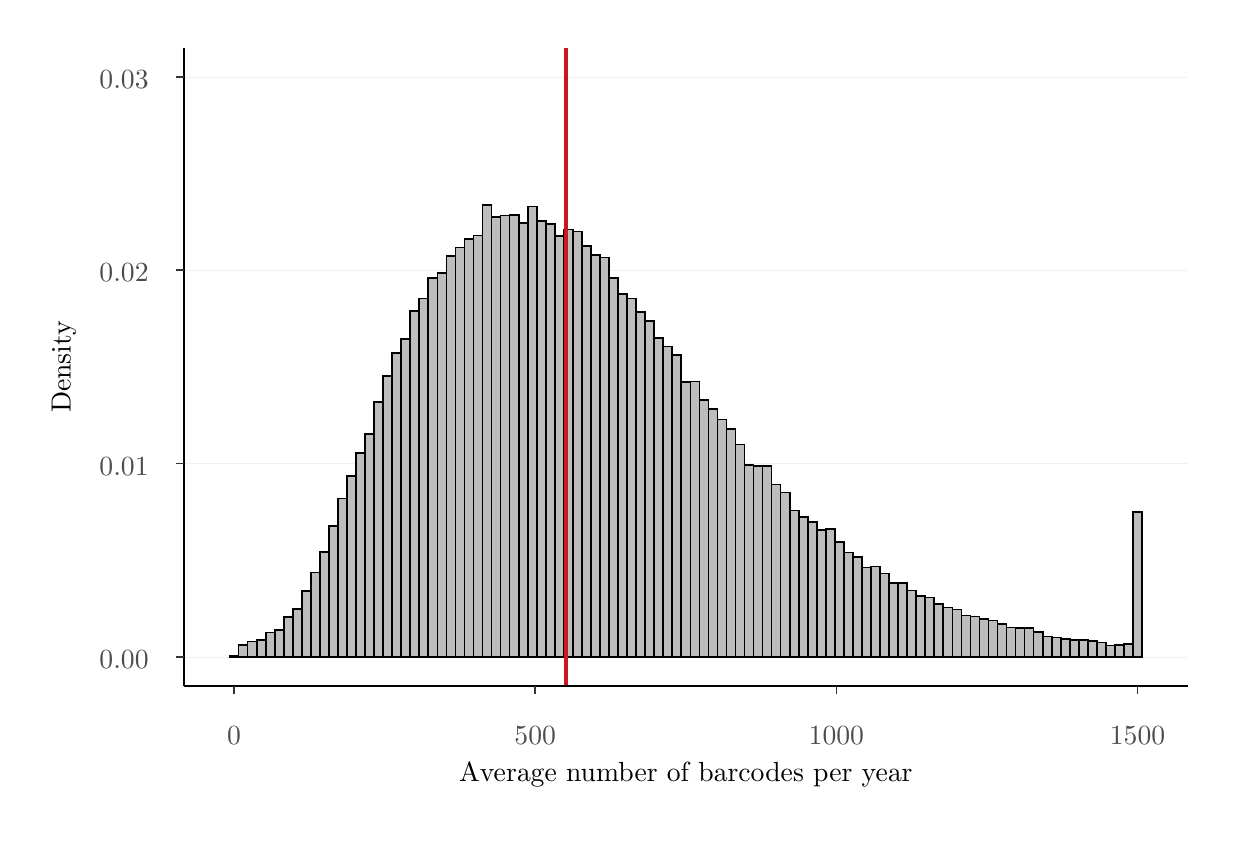
\begin{tikzpicture}[x=1pt,y=1pt]
\definecolor{fillColor}{RGB}{255,255,255}
\path[use as bounding box,fill=fillColor,fill opacity=0.00] (0,0) rectangle (433.62,289.08);
\begin{scope}
\path[clip] (  0.00,  0.00) rectangle (433.62,289.08);
\definecolor{drawColor}{RGB}{255,255,255}
\definecolor{fillColor}{RGB}{255,255,255}

\path[draw=drawColor,line width= 0.6pt,line join=round,line cap=round,fill=fillColor] ( -0.00,  0.00) rectangle (433.62,289.08);
\end{scope}
\begin{scope}
\path[clip] ( 56.47, 51.15) rectangle (419.17,281.85);
\definecolor{drawColor}{RGB}{255,255,255}

\path[draw=drawColor,line width= 0.3pt,line join=round] ( 56.47, 96.59) --
	(419.17, 96.59);

\path[draw=drawColor,line width= 0.3pt,line join=round] ( 56.47,166.50) --
	(419.17,166.50);

\path[draw=drawColor,line width= 0.3pt,line join=round] ( 56.47,236.41) --
	(419.17,236.41);

\path[draw=drawColor,line width= 0.3pt,line join=round] (128.99, 51.15) --
	(128.99,281.85);

\path[draw=drawColor,line width= 0.3pt,line join=round] (237.82, 51.15) --
	(237.82,281.85);

\path[draw=drawColor,line width= 0.3pt,line join=round] (346.64, 51.15) --
	(346.64,281.85);
\definecolor{drawColor}{gray}{0.94}

\path[draw=drawColor,line width= 0.1pt,line join=round] ( 56.47, 61.64) --
	(419.17, 61.64);

\path[draw=drawColor,line width= 0.1pt,line join=round] ( 56.47,131.55) --
	(419.17,131.55);

\path[draw=drawColor,line width= 0.1pt,line join=round] ( 56.47,201.46) --
	(419.17,201.46);

\path[draw=drawColor,line width= 0.1pt,line join=round] ( 56.47,271.37) --
	(419.17,271.37);
\definecolor{drawColor}{RGB}{0,0,0}
\definecolor{fillColor}{gray}{0.74}

\path[draw=drawColor,line width= 0.6pt,line cap=rect,fill=fillColor] ( 72.95, 61.64) rectangle ( 76.22, 62.06);

\path[draw=drawColor,line width= 0.6pt,line cap=rect,fill=fillColor] ( 76.22, 61.64) rectangle ( 79.48, 66.04);

\path[draw=drawColor,line width= 0.6pt,line cap=rect,fill=fillColor] ( 79.48, 61.64) rectangle ( 82.75, 67.30);

\path[draw=drawColor,line width= 0.6pt,line cap=rect,fill=fillColor] ( 82.75, 61.64) rectangle ( 86.01, 67.90);

\path[draw=drawColor,line width= 0.6pt,line cap=rect,fill=fillColor] ( 86.01, 61.64) rectangle ( 89.28, 70.47);

\path[draw=drawColor,line width= 0.6pt,line cap=rect,fill=fillColor] ( 89.28, 61.64) rectangle ( 92.54, 71.52);

\path[draw=drawColor,line width= 0.6pt,line cap=rect,fill=fillColor] ( 92.54, 61.64) rectangle ( 95.80, 76.22);

\path[draw=drawColor,line width= 0.6pt,line cap=rect,fill=fillColor] ( 95.80, 61.64) rectangle ( 99.07, 78.98);

\path[draw=drawColor,line width= 0.6pt,line cap=rect,fill=fillColor] ( 99.07, 61.64) rectangle (102.33, 85.59);

\path[draw=drawColor,line width= 0.6pt,line cap=rect,fill=fillColor] (102.33, 61.64) rectangle (105.60, 92.21);

\path[draw=drawColor,line width= 0.6pt,line cap=rect,fill=fillColor] (105.60, 61.64) rectangle (108.86, 99.64);

\path[draw=drawColor,line width= 0.6pt,line cap=rect,fill=fillColor] (108.86, 61.64) rectangle (112.13,109.07);

\path[draw=drawColor,line width= 0.6pt,line cap=rect,fill=fillColor] (112.13, 61.64) rectangle (115.39,118.98);

\path[draw=drawColor,line width= 0.6pt,line cap=rect,fill=fillColor] (115.39, 61.64) rectangle (118.66,127.12);

\path[draw=drawColor,line width= 0.6pt,line cap=rect,fill=fillColor] (118.66, 61.64) rectangle (121.92,135.45);

\path[draw=drawColor,line width= 0.6pt,line cap=rect,fill=fillColor] (121.92, 61.64) rectangle (125.19,142.21);

\path[draw=drawColor,line width= 0.6pt,line cap=rect,fill=fillColor] (125.19, 61.64) rectangle (128.45,153.80);

\path[draw=drawColor,line width= 0.6pt,line cap=rect,fill=fillColor] (128.45, 61.64) rectangle (131.72,163.26);

\path[draw=drawColor,line width= 0.6pt,line cap=rect,fill=fillColor] (131.72, 61.64) rectangle (134.98,171.53);

\path[draw=drawColor,line width= 0.6pt,line cap=rect,fill=fillColor] (134.98, 61.64) rectangle (138.24,176.47);

\path[draw=drawColor,line width= 0.6pt,line cap=rect,fill=fillColor] (138.24, 61.64) rectangle (141.51,186.80);

\path[draw=drawColor,line width= 0.6pt,line cap=rect,fill=fillColor] (141.51, 61.64) rectangle (144.77,191.17);

\path[draw=drawColor,line width= 0.6pt,line cap=rect,fill=fillColor] (144.77, 61.64) rectangle (148.04,198.54);

\path[draw=drawColor,line width= 0.6pt,line cap=rect,fill=fillColor] (148.04, 61.64) rectangle (151.30,200.39);

\path[draw=drawColor,line width= 0.6pt,line cap=rect,fill=fillColor] (151.30, 61.64) rectangle (154.57,206.68);

\path[draw=drawColor,line width= 0.6pt,line cap=rect,fill=fillColor] (154.57, 61.64) rectangle (157.83,209.64);

\path[draw=drawColor,line width= 0.6pt,line cap=rect,fill=fillColor] (157.83, 61.64) rectangle (161.10,212.67);

\path[draw=drawColor,line width= 0.6pt,line cap=rect,fill=fillColor] (161.10, 61.64) rectangle (164.36,213.93);

\path[draw=drawColor,line width= 0.6pt,line cap=rect,fill=fillColor] (164.36, 61.64) rectangle (167.63,225.00);

\path[draw=drawColor,line width= 0.6pt,line cap=rect,fill=fillColor] (167.63, 61.64) rectangle (170.89,220.72);

\path[draw=drawColor,line width= 0.6pt,line cap=rect,fill=fillColor] (170.89, 61.64) rectangle (174.16,221.23);

\path[draw=drawColor,line width= 0.6pt,line cap=rect,fill=fillColor] (174.16, 61.64) rectangle (177.42,221.41);

\path[draw=drawColor,line width= 0.6pt,line cap=rect,fill=fillColor] (177.42, 61.64) rectangle (180.68,218.48);

\path[draw=drawColor,line width= 0.6pt,line cap=rect,fill=fillColor] (180.68, 61.64) rectangle (183.95,224.44);

\path[draw=drawColor,line width= 0.6pt,line cap=rect,fill=fillColor] (183.95, 61.64) rectangle (187.21,219.26);

\path[draw=drawColor,line width= 0.6pt,line cap=rect,fill=fillColor] (187.21, 61.64) rectangle (190.48,218.15);

\path[draw=drawColor,line width= 0.6pt,line cap=rect,fill=fillColor] (190.48, 61.64) rectangle (193.74,213.81);

\path[draw=drawColor,line width= 0.6pt,line cap=rect,fill=fillColor] (193.74, 61.64) rectangle (197.01,216.11);

\path[draw=drawColor,line width= 0.6pt,line cap=rect,fill=fillColor] (197.01, 61.64) rectangle (200.27,215.39);

\path[draw=drawColor,line width= 0.6pt,line cap=rect,fill=fillColor] (200.27, 61.64) rectangle (203.54,210.27);

\path[draw=drawColor,line width= 0.6pt,line cap=rect,fill=fillColor] (203.54, 61.64) rectangle (206.80,206.98);

\path[draw=drawColor,line width= 0.6pt,line cap=rect,fill=fillColor] (206.80, 61.64) rectangle (210.07,206.05);

\path[draw=drawColor,line width= 0.6pt,line cap=rect,fill=fillColor] (210.07, 61.64) rectangle (213.33,198.66);

\path[draw=drawColor,line width= 0.6pt,line cap=rect,fill=fillColor] (213.33, 61.64) rectangle (216.60,192.85);

\path[draw=drawColor,line width= 0.6pt,line cap=rect,fill=fillColor] (216.60, 61.64) rectangle (219.86,191.26);

\path[draw=drawColor,line width= 0.6pt,line cap=rect,fill=fillColor] (219.86, 61.64) rectangle (223.13,186.23);

\path[draw=drawColor,line width= 0.6pt,line cap=rect,fill=fillColor] (223.13, 61.64) rectangle (226.39,183.12);

\path[draw=drawColor,line width= 0.6pt,line cap=rect,fill=fillColor] (226.39, 61.64) rectangle (229.65,176.95);

\path[draw=drawColor,line width= 0.6pt,line cap=rect,fill=fillColor] (229.65, 61.64) rectangle (232.92,173.89);

\path[draw=drawColor,line width= 0.6pt,line cap=rect,fill=fillColor] (232.92, 61.64) rectangle (236.18,170.72);

\path[draw=drawColor,line width= 0.6pt,line cap=rect,fill=fillColor] (236.18, 61.64) rectangle (239.45,160.99);

\path[draw=drawColor,line width= 0.6pt,line cap=rect,fill=fillColor] (239.45, 61.64) rectangle (242.71,161.26);

\path[draw=drawColor,line width= 0.6pt,line cap=rect,fill=fillColor] (242.71, 61.64) rectangle (245.98,154.49);

\path[draw=drawColor,line width= 0.6pt,line cap=rect,fill=fillColor] (245.98, 61.64) rectangle (249.24,151.26);

\path[draw=drawColor,line width= 0.6pt,line cap=rect,fill=fillColor] (249.24, 61.64) rectangle (252.51,147.48);

\path[draw=drawColor,line width= 0.6pt,line cap=rect,fill=fillColor] (252.51, 61.64) rectangle (255.77,144.10);

\path[draw=drawColor,line width= 0.6pt,line cap=rect,fill=fillColor] (255.77, 61.64) rectangle (259.04,138.44);

\path[draw=drawColor,line width= 0.6pt,line cap=rect,fill=fillColor] (259.04, 61.64) rectangle (262.30,131.02);

\path[draw=drawColor,line width= 0.6pt,line cap=rect,fill=fillColor] (262.30, 61.64) rectangle (265.57,130.66);

\path[draw=drawColor,line width= 0.6pt,line cap=rect,fill=fillColor] (265.57, 61.64) rectangle (268.83,130.78);

\path[draw=drawColor,line width= 0.6pt,line cap=rect,fill=fillColor] (268.83, 61.64) rectangle (272.09,124.01);

\path[draw=drawColor,line width= 0.6pt,line cap=rect,fill=fillColor] (272.09, 61.64) rectangle (275.36,121.11);

\path[draw=drawColor,line width= 0.6pt,line cap=rect,fill=fillColor] (275.36, 61.64) rectangle (278.62,114.55);

\path[draw=drawColor,line width= 0.6pt,line cap=rect,fill=fillColor] (278.62, 61.64) rectangle (281.89,112.33);

\path[draw=drawColor,line width= 0.6pt,line cap=rect,fill=fillColor] (281.89, 61.64) rectangle (285.15,110.51);

\path[draw=drawColor,line width= 0.6pt,line cap=rect,fill=fillColor] (285.15, 61.64) rectangle (288.42,107.60);

\path[draw=drawColor,line width= 0.6pt,line cap=rect,fill=fillColor] (288.42, 61.64) rectangle (291.68,107.84);

\path[draw=drawColor,line width= 0.6pt,line cap=rect,fill=fillColor] (291.68, 61.64) rectangle (294.95,103.20);

\path[draw=drawColor,line width= 0.6pt,line cap=rect,fill=fillColor] (294.95, 61.64) rectangle (298.21, 99.46);

\path[draw=drawColor,line width= 0.6pt,line cap=rect,fill=fillColor] (298.21, 61.64) rectangle (301.48, 97.78);

\path[draw=drawColor,line width= 0.6pt,line cap=rect,fill=fillColor] (301.48, 61.64) rectangle (304.74, 94.04);

\path[draw=drawColor,line width= 0.6pt,line cap=rect,fill=fillColor] (304.74, 61.64) rectangle (308.01, 94.43);

\path[draw=drawColor,line width= 0.6pt,line cap=rect,fill=fillColor] (308.01, 61.64) rectangle (311.27, 91.79);

\path[draw=drawColor,line width= 0.6pt,line cap=rect,fill=fillColor] (311.27, 61.64) rectangle (314.53, 88.47);

\path[draw=drawColor,line width= 0.6pt,line cap=rect,fill=fillColor] (314.53, 61.64) rectangle (317.80, 88.41);

\path[draw=drawColor,line width= 0.6pt,line cap=rect,fill=fillColor] (317.80, 61.64) rectangle (321.06, 85.74);

\path[draw=drawColor,line width= 0.6pt,line cap=rect,fill=fillColor] (321.06, 61.64) rectangle (324.33, 83.62);

\path[draw=drawColor,line width= 0.6pt,line cap=rect,fill=fillColor] (324.33, 61.64) rectangle (327.59, 83.14);

\path[draw=drawColor,line width= 0.6pt,line cap=rect,fill=fillColor] (327.59, 61.64) rectangle (330.86, 80.77);

\path[draw=drawColor,line width= 0.6pt,line cap=rect,fill=fillColor] (330.86, 61.64) rectangle (334.12, 79.58);

\path[draw=drawColor,line width= 0.6pt,line cap=rect,fill=fillColor] (334.12, 61.64) rectangle (337.39, 78.89);

\path[draw=drawColor,line width= 0.6pt,line cap=rect,fill=fillColor] (337.39, 61.64) rectangle (340.65, 76.67);

\path[draw=drawColor,line width= 0.6pt,line cap=rect,fill=fillColor] (340.65, 61.64) rectangle (343.92, 76.28);

\path[draw=drawColor,line width= 0.6pt,line cap=rect,fill=fillColor] (343.92, 61.64) rectangle (347.18, 75.41);

\path[draw=drawColor,line width= 0.6pt,line cap=rect,fill=fillColor] (347.18, 61.64) rectangle (350.45, 74.81);

\path[draw=drawColor,line width= 0.6pt,line cap=rect,fill=fillColor] (350.45, 61.64) rectangle (353.71, 73.56);

\path[draw=drawColor,line width= 0.6pt,line cap=rect,fill=fillColor] (353.71, 61.64) rectangle (356.97, 72.27);

\path[draw=drawColor,line width= 0.6pt,line cap=rect,fill=fillColor] (356.97, 61.64) rectangle (360.24, 72.09);

\path[draw=drawColor,line width= 0.6pt,line cap=rect,fill=fillColor] (360.24, 61.64) rectangle (363.50, 72.15);

\path[draw=drawColor,line width= 0.6pt,line cap=rect,fill=fillColor] (363.50, 61.64) rectangle (366.77, 70.80);

\path[draw=drawColor,line width= 0.6pt,line cap=rect,fill=fillColor] (366.77, 61.64) rectangle (370.03, 69.07);

\path[draw=drawColor,line width= 0.6pt,line cap=rect,fill=fillColor] (370.03, 61.64) rectangle (373.30, 68.68);

\path[draw=drawColor,line width= 0.6pt,line cap=rect,fill=fillColor] (373.30, 61.64) rectangle (376.56, 68.11);

\path[draw=drawColor,line width= 0.6pt,line cap=rect,fill=fillColor] (376.56, 61.64) rectangle (379.83, 67.90);

\path[draw=drawColor,line width= 0.6pt,line cap=rect,fill=fillColor] (379.83, 61.64) rectangle (383.09, 67.75);

\path[draw=drawColor,line width= 0.6pt,line cap=rect,fill=fillColor] (383.09, 61.64) rectangle (386.36, 67.54);

\path[draw=drawColor,line width= 0.6pt,line cap=rect,fill=fillColor] (386.36, 61.64) rectangle (389.62, 66.97);

\path[draw=drawColor,line width= 0.6pt,line cap=rect,fill=fillColor] (389.62, 61.64) rectangle (392.89, 65.77);

\path[draw=drawColor,line width= 0.6pt,line cap=rect,fill=fillColor] (392.89, 61.64) rectangle (396.15, 66.04);

\path[draw=drawColor,line width= 0.6pt,line cap=rect,fill=fillColor] (396.15, 61.64) rectangle (399.41, 66.25);

\path[draw=drawColor,line width= 0.6pt,line cap=rect,fill=fillColor] (399.41, 61.64) rectangle (402.68,114.10);
\definecolor{drawColor}{RGB}{203,24,29}

\path[draw=drawColor,line width= 1.7pt,line join=round] (194.51, 51.15) -- (194.51,281.85);
\end{scope}
\begin{scope}
\path[clip] (  0.00,  0.00) rectangle (433.62,289.08);
\definecolor{drawColor}{RGB}{0,0,0}

\path[draw=drawColor,line width= 0.6pt,line join=round] ( 56.47, 51.15) --
	( 56.47,281.85);
\end{scope}
\begin{scope}
\path[clip] (  0.00,  0.00) rectangle (433.62,289.08);
\definecolor{drawColor}{gray}{0.30}

\node[text=drawColor,anchor=base east,inner sep=0pt, outer sep=0pt, scale=  1.00] at ( 43.72, 57.51) {0.00};

\node[text=drawColor,anchor=base east,inner sep=0pt, outer sep=0pt, scale=  1.00] at ( 43.72,127.42) {0.01};

\node[text=drawColor,anchor=base east,inner sep=0pt, outer sep=0pt, scale=  1.00] at ( 43.72,197.32) {0.02};

\node[text=drawColor,anchor=base east,inner sep=0pt, outer sep=0pt, scale=  1.00] at ( 43.72,267.23) {0.03};
\end{scope}
\begin{scope}
\path[clip] (  0.00,  0.00) rectangle (433.62,289.08);
\definecolor{drawColor}{gray}{0.20}

\path[draw=drawColor,line width= 0.6pt,line join=round] ( 53.72, 61.64) --
	( 56.47, 61.64);

\path[draw=drawColor,line width= 0.6pt,line join=round] ( 53.72,131.55) --
	( 56.47,131.55);

\path[draw=drawColor,line width= 0.6pt,line join=round] ( 53.72,201.46) --
	( 56.47,201.46);

\path[draw=drawColor,line width= 0.6pt,line join=round] ( 53.72,271.37) --
	( 56.47,271.37);
\end{scope}
\begin{scope}
\path[clip] (  0.00,  0.00) rectangle (433.62,289.08);
\definecolor{drawColor}{RGB}{0,0,0}

\path[draw=drawColor,line width= 0.6pt,line join=round] ( 56.47, 51.15) --
	(419.17, 51.15);
\end{scope}
\begin{scope}
\path[clip] (  0.00,  0.00) rectangle (433.62,289.08);
\definecolor{drawColor}{gray}{0.20}

\path[draw=drawColor,line width= 0.6pt,line join=round] ( 74.58, 48.40) --
	( 74.58, 51.15);

\path[draw=drawColor,line width= 0.6pt,line join=round] (183.41, 48.40) --
	(183.41, 51.15);

\path[draw=drawColor,line width= 0.6pt,line join=round] (292.23, 48.40) --
	(292.23, 51.15);

\path[draw=drawColor,line width= 0.6pt,line join=round] (401.05, 48.40) --
	(401.05, 51.15);
\end{scope}
\begin{scope}
\path[clip] (  0.00,  0.00) rectangle (433.62,289.08);
\definecolor{drawColor}{gray}{0.30}

\node[text=drawColor,anchor=base,inner sep=0pt, outer sep=0pt, scale=  1.00] at ( 74.58, 30.14) {0};

\node[text=drawColor,anchor=base,inner sep=0pt, outer sep=0pt, scale=  1.00] at (183.41, 30.14) {500};

\node[text=drawColor,anchor=base,inner sep=0pt, outer sep=0pt, scale=  1.00] at (292.23, 30.14) {1000};

\node[text=drawColor,anchor=base,inner sep=0pt, outer sep=0pt, scale=  1.00] at (401.05, 30.14) {1500};
\end{scope}
\begin{scope}
\path[clip] (  0.00,  0.00) rectangle (433.62,289.08);
\definecolor{drawColor}{RGB}{0,0,0}

\node[text=drawColor,anchor=base,inner sep=0pt, outer sep=0pt, scale=  1.00] at (237.82, 16.79) {Average number of barcodes per year};
\end{scope}
\begin{scope}
\path[clip] (  0.00,  0.00) rectangle (433.62,289.08);
\definecolor{drawColor}{RGB}{0,0,0}

\node[text=drawColor,rotate= 90.00,anchor=base,inner sep=0pt, outer sep=0pt, scale=  1.00] at ( 15.49,166.50) {Density};
\end{scope}
\end{tikzpicture}
}
     \end{subfigure}
     \begin{subfigure}[t]{.49\textwidth}
         \centering
         \caption{The Netherlands}
         \scalebox{0.45}{% Created by tikzDevice version 0.12.3.1 on 2022-07-29 15:13:39
% !TEX encoding = UTF-8 Unicode
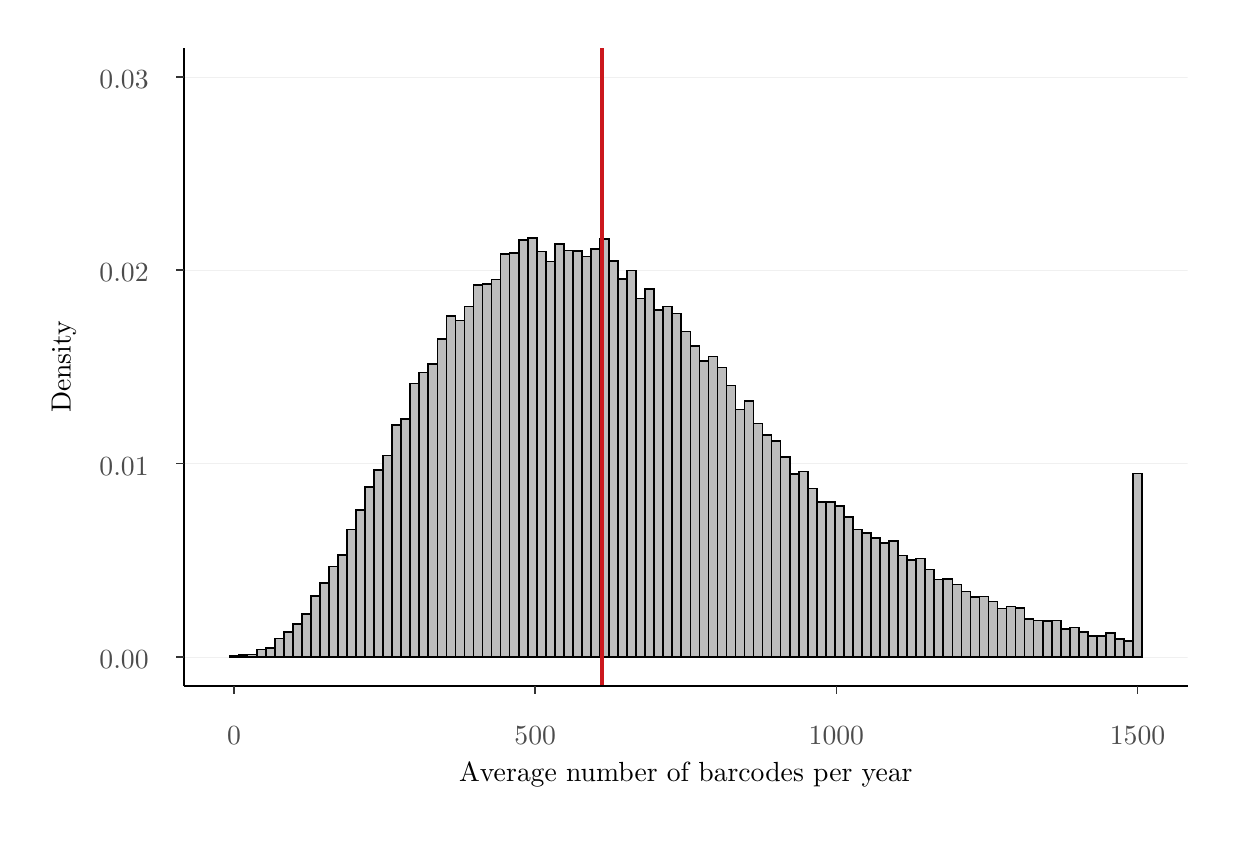
\begin{tikzpicture}[x=1pt,y=1pt]
\definecolor{fillColor}{RGB}{255,255,255}
\path[use as bounding box,fill=fillColor,fill opacity=0.00] (0,0) rectangle (433.62,289.08);
\begin{scope}
\path[clip] (  0.00,  0.00) rectangle (433.62,289.08);
\definecolor{drawColor}{RGB}{255,255,255}
\definecolor{fillColor}{RGB}{255,255,255}

\path[draw=drawColor,line width= 0.6pt,line join=round,line cap=round,fill=fillColor] ( -0.00,  0.00) rectangle (433.62,289.08);
\end{scope}
\begin{scope}
\path[clip] ( 56.47, 51.15) rectangle (419.17,281.85);
\definecolor{drawColor}{RGB}{255,255,255}

\path[draw=drawColor,line width= 0.3pt,line join=round] ( 56.47, 96.59) --
	(419.17, 96.59);

\path[draw=drawColor,line width= 0.3pt,line join=round] ( 56.47,166.50) --
	(419.17,166.50);

\path[draw=drawColor,line width= 0.3pt,line join=round] ( 56.47,236.41) --
	(419.17,236.41);

\path[draw=drawColor,line width= 0.3pt,line join=round] (128.99, 51.15) --
	(128.99,281.85);

\path[draw=drawColor,line width= 0.3pt,line join=round] (237.82, 51.15) --
	(237.82,281.85);

\path[draw=drawColor,line width= 0.3pt,line join=round] (346.64, 51.15) --
	(346.64,281.85);
\definecolor{drawColor}{gray}{0.94}

\path[draw=drawColor,line width= 0.1pt,line join=round] ( 56.47, 61.64) --
	(419.17, 61.64);

\path[draw=drawColor,line width= 0.1pt,line join=round] ( 56.47,131.55) --
	(419.17,131.55);

\path[draw=drawColor,line width= 0.1pt,line join=round] ( 56.47,201.46) --
	(419.17,201.46);

\path[draw=drawColor,line width= 0.1pt,line join=round] ( 56.47,271.37) --
	(419.17,271.37);
\definecolor{drawColor}{RGB}{0,0,0}
\definecolor{fillColor}{gray}{0.74}

\path[draw=drawColor,line width= 0.6pt,line cap=rect,fill=fillColor] ( 72.95, 61.64) rectangle ( 76.22, 62.05);

\path[draw=drawColor,line width= 0.6pt,line cap=rect,fill=fillColor] ( 76.22, 61.64) rectangle ( 79.48, 62.38);

\path[draw=drawColor,line width= 0.6pt,line cap=rect,fill=fillColor] ( 79.48, 61.64) rectangle ( 82.75, 62.63);

\path[draw=drawColor,line width= 0.6pt,line cap=rect,fill=fillColor] ( 82.75, 61.64) rectangle ( 86.01, 64.36);

\path[draw=drawColor,line width= 0.6pt,line cap=rect,fill=fillColor] ( 86.01, 61.64) rectangle ( 89.28, 64.94);

\path[draw=drawColor,line width= 0.6pt,line cap=rect,fill=fillColor] ( 89.28, 61.64) rectangle ( 92.54, 68.41);

\path[draw=drawColor,line width= 0.6pt,line cap=rect,fill=fillColor] ( 92.54, 61.64) rectangle ( 95.80, 70.72);

\path[draw=drawColor,line width= 0.6pt,line cap=rect,fill=fillColor] ( 95.80, 61.64) rectangle ( 99.07, 73.61);

\path[draw=drawColor,line width= 0.6pt,line cap=rect,fill=fillColor] ( 99.07, 61.64) rectangle (102.33, 77.16);

\path[draw=drawColor,line width= 0.6pt,line cap=rect,fill=fillColor] (102.33, 61.64) rectangle (105.60, 83.68);

\path[draw=drawColor,line width= 0.6pt,line cap=rect,fill=fillColor] (105.60, 61.64) rectangle (108.86, 88.47);

\path[draw=drawColor,line width= 0.6pt,line cap=rect,fill=fillColor] (108.86, 61.64) rectangle (112.13, 94.42);

\path[draw=drawColor,line width= 0.6pt,line cap=rect,fill=fillColor] (112.13, 61.64) rectangle (115.39, 98.46);

\path[draw=drawColor,line width= 0.6pt,line cap=rect,fill=fillColor] (115.39, 61.64) rectangle (118.66,107.79);

\path[draw=drawColor,line width= 0.6pt,line cap=rect,fill=fillColor] (118.66, 61.64) rectangle (121.92,114.73);

\path[draw=drawColor,line width= 0.6pt,line cap=rect,fill=fillColor] (121.92, 61.64) rectangle (125.19,123.15);

\path[draw=drawColor,line width= 0.6pt,line cap=rect,fill=fillColor] (125.19, 61.64) rectangle (128.45,129.26);

\path[draw=drawColor,line width= 0.6pt,line cap=rect,fill=fillColor] (128.45, 61.64) rectangle (131.72,134.54);

\path[draw=drawColor,line width= 0.6pt,line cap=rect,fill=fillColor] (131.72, 61.64) rectangle (134.98,145.44);

\path[draw=drawColor,line width= 0.6pt,line cap=rect,fill=fillColor] (134.98, 61.64) rectangle (138.24,147.67);

\path[draw=drawColor,line width= 0.6pt,line cap=rect,fill=fillColor] (138.24, 61.64) rectangle (141.51,160.55);

\path[draw=drawColor,line width= 0.6pt,line cap=rect,fill=fillColor] (141.51, 61.64) rectangle (144.77,164.51);

\path[draw=drawColor,line width= 0.6pt,line cap=rect,fill=fillColor] (144.77, 61.64) rectangle (148.04,167.56);

\path[draw=drawColor,line width= 0.6pt,line cap=rect,fill=fillColor] (148.04, 61.64) rectangle (151.30,176.56);

\path[draw=drawColor,line width= 0.6pt,line cap=rect,fill=fillColor] (151.30, 61.64) rectangle (154.57,184.90);

\path[draw=drawColor,line width= 0.6pt,line cap=rect,fill=fillColor] (154.57, 61.64) rectangle (157.83,183.25);

\path[draw=drawColor,line width= 0.6pt,line cap=rect,fill=fillColor] (157.83, 61.64) rectangle (161.10,188.28);

\path[draw=drawColor,line width= 0.6pt,line cap=rect,fill=fillColor] (161.10, 61.64) rectangle (164.36,196.05);

\path[draw=drawColor,line width= 0.6pt,line cap=rect,fill=fillColor] (164.36, 61.64) rectangle (167.63,196.46);

\path[draw=drawColor,line width= 0.6pt,line cap=rect,fill=fillColor] (167.63, 61.64) rectangle (170.89,198.03);

\path[draw=drawColor,line width= 0.6pt,line cap=rect,fill=fillColor] (170.89, 61.64) rectangle (174.16,207.36);

\path[draw=drawColor,line width= 0.6pt,line cap=rect,fill=fillColor] (174.16, 61.64) rectangle (177.42,207.60);

\path[draw=drawColor,line width= 0.6pt,line cap=rect,fill=fillColor] (177.42, 61.64) rectangle (180.68,212.31);

\path[draw=drawColor,line width= 0.6pt,line cap=rect,fill=fillColor] (180.68, 61.64) rectangle (183.95,213.05);

\path[draw=drawColor,line width= 0.6pt,line cap=rect,fill=fillColor] (183.95, 61.64) rectangle (187.21,208.18);

\path[draw=drawColor,line width= 0.6pt,line cap=rect,fill=fillColor] (187.21, 61.64) rectangle (190.48,204.55);

\path[draw=drawColor,line width= 0.6pt,line cap=rect,fill=fillColor] (190.48, 61.64) rectangle (193.74,210.91);

\path[draw=drawColor,line width= 0.6pt,line cap=rect,fill=fillColor] (193.74, 61.64) rectangle (197.01,208.51);

\path[draw=drawColor,line width= 0.6pt,line cap=rect,fill=fillColor] (197.01, 61.64) rectangle (200.27,208.35);

\path[draw=drawColor,line width= 0.6pt,line cap=rect,fill=fillColor] (200.27, 61.64) rectangle (203.54,206.45);

\path[draw=drawColor,line width= 0.6pt,line cap=rect,fill=fillColor] (203.54, 61.64) rectangle (206.80,209.09);

\path[draw=drawColor,line width= 0.6pt,line cap=rect,fill=fillColor] (206.80, 61.64) rectangle (210.07,212.72);

\path[draw=drawColor,line width= 0.6pt,line cap=rect,fill=fillColor] (210.07, 61.64) rectangle (213.33,204.80);

\path[draw=drawColor,line width= 0.6pt,line cap=rect,fill=fillColor] (213.33, 61.64) rectangle (216.60,198.19);

\path[draw=drawColor,line width= 0.6pt,line cap=rect,fill=fillColor] (216.60, 61.64) rectangle (219.86,201.33);

\path[draw=drawColor,line width= 0.6pt,line cap=rect,fill=fillColor] (219.86, 61.64) rectangle (223.13,191.26);

\path[draw=drawColor,line width= 0.6pt,line cap=rect,fill=fillColor] (223.13, 61.64) rectangle (226.39,194.56);

\path[draw=drawColor,line width= 0.6pt,line cap=rect,fill=fillColor] (226.39, 61.64) rectangle (229.65,187.05);

\path[draw=drawColor,line width= 0.6pt,line cap=rect,fill=fillColor] (229.65, 61.64) rectangle (232.92,188.37);

\path[draw=drawColor,line width= 0.6pt,line cap=rect,fill=fillColor] (232.92, 61.64) rectangle (236.18,185.81);

\path[draw=drawColor,line width= 0.6pt,line cap=rect,fill=fillColor] (236.18, 61.64) rectangle (239.45,179.29);

\path[draw=drawColor,line width= 0.6pt,line cap=rect,fill=fillColor] (239.45, 61.64) rectangle (242.71,174.08);

\path[draw=drawColor,line width= 0.6pt,line cap=rect,fill=fillColor] (242.71, 61.64) rectangle (245.98,168.64);

\path[draw=drawColor,line width= 0.6pt,line cap=rect,fill=fillColor] (245.98, 61.64) rectangle (249.24,170.20);

\path[draw=drawColor,line width= 0.6pt,line cap=rect,fill=fillColor] (249.24, 61.64) rectangle (252.51,166.24);

\path[draw=drawColor,line width= 0.6pt,line cap=rect,fill=fillColor] (252.51, 61.64) rectangle (255.77,159.80);

\path[draw=drawColor,line width= 0.6pt,line cap=rect,fill=fillColor] (255.77, 61.64) rectangle (259.04,151.13);

\path[draw=drawColor,line width= 0.6pt,line cap=rect,fill=fillColor] (259.04, 61.64) rectangle (262.30,154.11);

\path[draw=drawColor,line width= 0.6pt,line cap=rect,fill=fillColor] (262.30, 61.64) rectangle (265.57,146.01);

\path[draw=drawColor,line width= 0.6pt,line cap=rect,fill=fillColor] (265.57, 61.64) rectangle (268.83,141.97);

\path[draw=drawColor,line width= 0.6pt,line cap=rect,fill=fillColor] (268.83, 61.64) rectangle (272.09,139.74);

\path[draw=drawColor,line width= 0.6pt,line cap=rect,fill=fillColor] (272.09, 61.64) rectangle (275.36,134.04);

\path[draw=drawColor,line width= 0.6pt,line cap=rect,fill=fillColor] (275.36, 61.64) rectangle (278.62,127.85);

\path[draw=drawColor,line width= 0.6pt,line cap=rect,fill=fillColor] (278.62, 61.64) rectangle (281.89,128.76);

\path[draw=drawColor,line width= 0.6pt,line cap=rect,fill=fillColor] (281.89, 61.64) rectangle (285.15,122.57);

\path[draw=drawColor,line width= 0.6pt,line cap=rect,fill=fillColor] (285.15, 61.64) rectangle (288.42,117.61);

\path[draw=drawColor,line width= 0.6pt,line cap=rect,fill=fillColor] (288.42, 61.64) rectangle (291.68,117.78);

\path[draw=drawColor,line width= 0.6pt,line cap=rect,fill=fillColor] (291.68, 61.64) rectangle (294.95,116.21);

\path[draw=drawColor,line width= 0.6pt,line cap=rect,fill=fillColor] (294.95, 61.64) rectangle (298.21,112.25);

\path[draw=drawColor,line width= 0.6pt,line cap=rect,fill=fillColor] (298.21, 61.64) rectangle (301.48,107.79);

\path[draw=drawColor,line width= 0.6pt,line cap=rect,fill=fillColor] (301.48, 61.64) rectangle (304.74,106.39);

\path[draw=drawColor,line width= 0.6pt,line cap=rect,fill=fillColor] (304.74, 61.64) rectangle (308.01,104.65);

\path[draw=drawColor,line width= 0.6pt,line cap=rect,fill=fillColor] (308.01, 61.64) rectangle (311.27,102.84);

\path[draw=drawColor,line width= 0.6pt,line cap=rect,fill=fillColor] (311.27, 61.64) rectangle (314.53,103.58);

\path[draw=drawColor,line width= 0.6pt,line cap=rect,fill=fillColor] (314.53, 61.64) rectangle (317.80, 98.30);

\path[draw=drawColor,line width= 0.6pt,line cap=rect,fill=fillColor] (317.80, 61.64) rectangle (321.06, 96.81);

\path[draw=drawColor,line width= 0.6pt,line cap=rect,fill=fillColor] (321.06, 61.64) rectangle (324.33, 97.22);

\path[draw=drawColor,line width= 0.6pt,line cap=rect,fill=fillColor] (324.33, 61.64) rectangle (327.59, 93.34);

\path[draw=drawColor,line width= 0.6pt,line cap=rect,fill=fillColor] (327.59, 61.64) rectangle (330.86, 89.71);

\path[draw=drawColor,line width= 0.6pt,line cap=rect,fill=fillColor] (330.86, 61.64) rectangle (334.12, 89.79);

\path[draw=drawColor,line width= 0.6pt,line cap=rect,fill=fillColor] (334.12, 61.64) rectangle (337.39, 87.89);

\path[draw=drawColor,line width= 0.6pt,line cap=rect,fill=fillColor] (337.39, 61.64) rectangle (340.65, 85.33);

\path[draw=drawColor,line width= 0.6pt,line cap=rect,fill=fillColor] (340.65, 61.64) rectangle (343.92, 83.27);

\path[draw=drawColor,line width= 0.6pt,line cap=rect,fill=fillColor] (343.92, 61.64) rectangle (347.18, 83.52);

\path[draw=drawColor,line width= 0.6pt,line cap=rect,fill=fillColor] (347.18, 61.64) rectangle (350.45, 81.78);

\path[draw=drawColor,line width= 0.6pt,line cap=rect,fill=fillColor] (350.45, 61.64) rectangle (353.71, 79.22);

\path[draw=drawColor,line width= 0.6pt,line cap=rect,fill=fillColor] (353.71, 61.64) rectangle (356.97, 79.89);

\path[draw=drawColor,line width= 0.6pt,line cap=rect,fill=fillColor] (356.97, 61.64) rectangle (360.24, 79.39);

\path[draw=drawColor,line width= 0.6pt,line cap=rect,fill=fillColor] (360.24, 61.64) rectangle (363.50, 75.51);

\path[draw=drawColor,line width= 0.6pt,line cap=rect,fill=fillColor] (363.50, 61.64) rectangle (366.77, 74.85);

\path[draw=drawColor,line width= 0.6pt,line cap=rect,fill=fillColor] (366.77, 61.64) rectangle (370.03, 74.60);

\path[draw=drawColor,line width= 0.6pt,line cap=rect,fill=fillColor] (370.03, 61.64) rectangle (373.30, 74.85);

\path[draw=drawColor,line width= 0.6pt,line cap=rect,fill=fillColor] (373.30, 61.64) rectangle (376.56, 71.88);

\path[draw=drawColor,line width= 0.6pt,line cap=rect,fill=fillColor] (376.56, 61.64) rectangle (379.83, 72.29);

\path[draw=drawColor,line width= 0.6pt,line cap=rect,fill=fillColor] (379.83, 61.64) rectangle (383.09, 70.72);

\path[draw=drawColor,line width= 0.6pt,line cap=rect,fill=fillColor] (383.09, 61.64) rectangle (386.36, 69.15);

\path[draw=drawColor,line width= 0.6pt,line cap=rect,fill=fillColor] (386.36, 61.64) rectangle (389.62, 69.32);

\path[draw=drawColor,line width= 0.6pt,line cap=rect,fill=fillColor] (389.62, 61.64) rectangle (392.89, 70.23);

\path[draw=drawColor,line width= 0.6pt,line cap=rect,fill=fillColor] (392.89, 61.64) rectangle (396.15, 68.16);

\path[draw=drawColor,line width= 0.6pt,line cap=rect,fill=fillColor] (396.15, 61.64) rectangle (399.41, 67.50);

\path[draw=drawColor,line width= 0.6pt,line cap=rect,fill=fillColor] (399.41, 61.64) rectangle (402.68,128.02);
\definecolor{drawColor}{RGB}{203,24,29}

\path[draw=drawColor,line width= 1.7pt,line join=round] (207.56, 51.15) -- (207.56,281.85);
\end{scope}
\begin{scope}
\path[clip] (  0.00,  0.00) rectangle (433.62,289.08);
\definecolor{drawColor}{RGB}{0,0,0}

\path[draw=drawColor,line width= 0.6pt,line join=round] ( 56.47, 51.15) --
	( 56.47,281.85);
\end{scope}
\begin{scope}
\path[clip] (  0.00,  0.00) rectangle (433.62,289.08);
\definecolor{drawColor}{gray}{0.30}

\node[text=drawColor,anchor=base east,inner sep=0pt, outer sep=0pt, scale=  1.00] at ( 43.72, 57.51) {0.00};

\node[text=drawColor,anchor=base east,inner sep=0pt, outer sep=0pt, scale=  1.00] at ( 43.72,127.42) {0.01};

\node[text=drawColor,anchor=base east,inner sep=0pt, outer sep=0pt, scale=  1.00] at ( 43.72,197.32) {0.02};

\node[text=drawColor,anchor=base east,inner sep=0pt, outer sep=0pt, scale=  1.00] at ( 43.72,267.23) {0.03};
\end{scope}
\begin{scope}
\path[clip] (  0.00,  0.00) rectangle (433.62,289.08);
\definecolor{drawColor}{gray}{0.20}

\path[draw=drawColor,line width= 0.6pt,line join=round] ( 53.72, 61.64) --
	( 56.47, 61.64);

\path[draw=drawColor,line width= 0.6pt,line join=round] ( 53.72,131.55) --
	( 56.47,131.55);

\path[draw=drawColor,line width= 0.6pt,line join=round] ( 53.72,201.46) --
	( 56.47,201.46);

\path[draw=drawColor,line width= 0.6pt,line join=round] ( 53.72,271.37) --
	( 56.47,271.37);
\end{scope}
\begin{scope}
\path[clip] (  0.00,  0.00) rectangle (433.62,289.08);
\definecolor{drawColor}{RGB}{0,0,0}

\path[draw=drawColor,line width= 0.6pt,line join=round] ( 56.47, 51.15) --
	(419.17, 51.15);
\end{scope}
\begin{scope}
\path[clip] (  0.00,  0.00) rectangle (433.62,289.08);
\definecolor{drawColor}{gray}{0.20}

\path[draw=drawColor,line width= 0.6pt,line join=round] ( 74.58, 48.40) --
	( 74.58, 51.15);

\path[draw=drawColor,line width= 0.6pt,line join=round] (183.41, 48.40) --
	(183.41, 51.15);

\path[draw=drawColor,line width= 0.6pt,line join=round] (292.23, 48.40) --
	(292.23, 51.15);

\path[draw=drawColor,line width= 0.6pt,line join=round] (401.05, 48.40) --
	(401.05, 51.15);
\end{scope}
\begin{scope}
\path[clip] (  0.00,  0.00) rectangle (433.62,289.08);
\definecolor{drawColor}{gray}{0.30}

\node[text=drawColor,anchor=base,inner sep=0pt, outer sep=0pt, scale=  1.00] at ( 74.58, 30.14) {0};

\node[text=drawColor,anchor=base,inner sep=0pt, outer sep=0pt, scale=  1.00] at (183.41, 30.14) {500};

\node[text=drawColor,anchor=base,inner sep=0pt, outer sep=0pt, scale=  1.00] at (292.23, 30.14) {1000};

\node[text=drawColor,anchor=base,inner sep=0pt, outer sep=0pt, scale=  1.00] at (401.05, 30.14) {1500};
\end{scope}
\begin{scope}
\path[clip] (  0.00,  0.00) rectangle (433.62,289.08);
\definecolor{drawColor}{RGB}{0,0,0}

\node[text=drawColor,anchor=base,inner sep=0pt, outer sep=0pt, scale=  1.00] at (237.82, 16.79) {Average number of barcodes per year};
\end{scope}
\begin{scope}
\path[clip] (  0.00,  0.00) rectangle (433.62,289.08);
\definecolor{drawColor}{RGB}{0,0,0}

\node[text=drawColor,rotate= 90.00,anchor=base,inner sep=0pt, outer sep=0pt, scale=  1.00] at ( 15.49,166.50) {Density};
\end{scope}
\end{tikzpicture}
}
     \end{subfigure}
     \parbox{\textwidth}{
        \begin{spacing}{1} 
            {\footnotesize 
            \textit{Notes}: These figures plot the distribution of the average number of consumed barcodes per year across households in the final sample on the 68 included product categories for each country.}
        \end{spacing}}
 \end{figure} 

 \begin{figure}[H]
    \centering
    \caption{Purchases per week}
    \label{fig: app_data_households_trans_year}
    \begin{subfigure}[t]{.49\textwidth}
         \centering
         \caption{Belgium}
         \scalebox{0.45}{% Created by tikzDevice version 0.12.3.1 on 2022-07-29 15:13:39
% !TEX encoding = UTF-8 Unicode
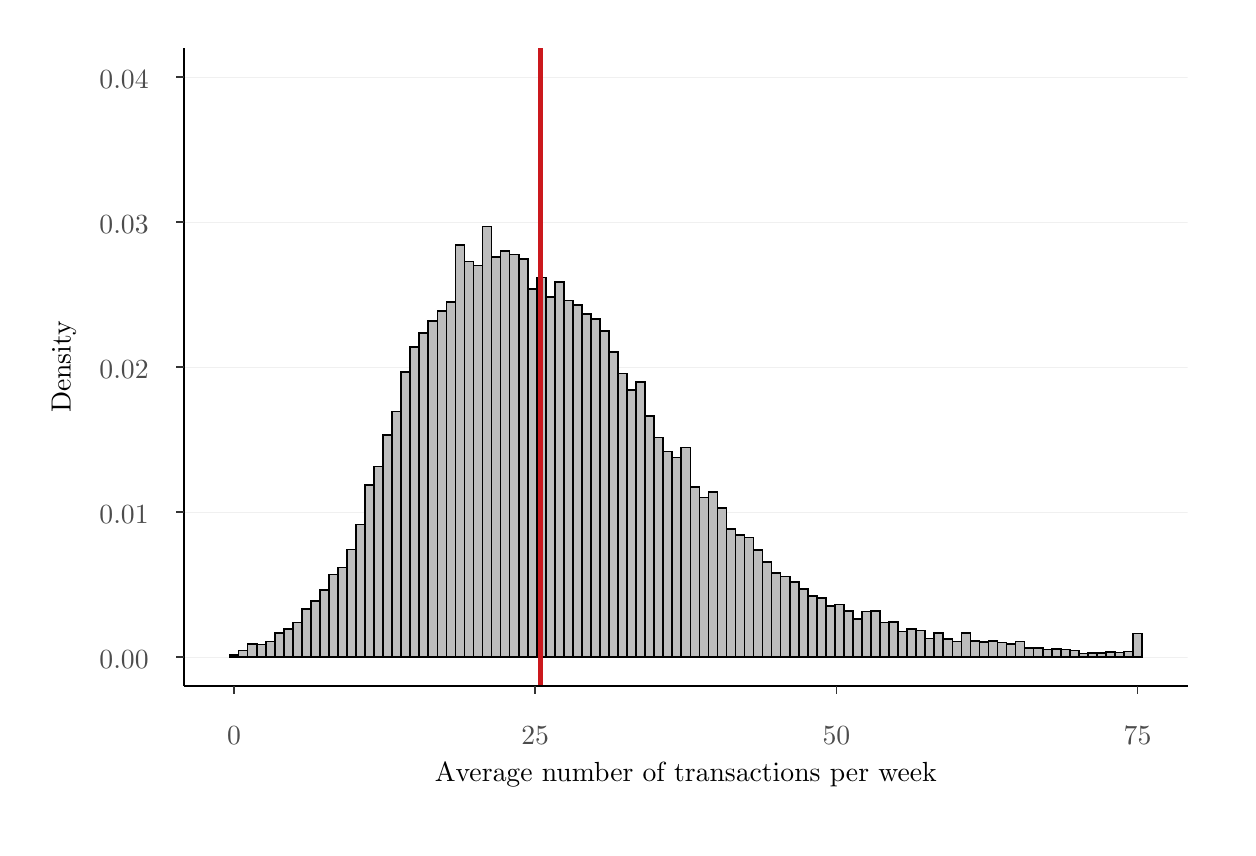
\begin{tikzpicture}[x=1pt,y=1pt]
\definecolor{fillColor}{RGB}{255,255,255}
\path[use as bounding box,fill=fillColor,fill opacity=0.00] (0,0) rectangle (433.62,289.08);
\begin{scope}
\path[clip] (  0.00,  0.00) rectangle (433.62,289.08);
\definecolor{drawColor}{RGB}{255,255,255}
\definecolor{fillColor}{RGB}{255,255,255}

\path[draw=drawColor,line width= 0.6pt,line join=round,line cap=round,fill=fillColor] ( -0.00,  0.00) rectangle (433.62,289.08);
\end{scope}
\begin{scope}
\path[clip] ( 56.47, 51.15) rectangle (419.17,281.85);
\definecolor{drawColor}{RGB}{255,255,255}

\path[draw=drawColor,line width= 0.3pt,line join=round] ( 56.47, 87.86) --
	(419.17, 87.86);

\path[draw=drawColor,line width= 0.3pt,line join=round] ( 56.47,140.29) --
	(419.17,140.29);

\path[draw=drawColor,line width= 0.3pt,line join=round] ( 56.47,192.72) --
	(419.17,192.72);

\path[draw=drawColor,line width= 0.3pt,line join=round] ( 56.47,245.15) --
	(419.17,245.15);

\path[draw=drawColor,line width= 0.3pt,line join=round] (128.99, 51.15) --
	(128.99,281.85);

\path[draw=drawColor,line width= 0.3pt,line join=round] (237.82, 51.15) --
	(237.82,281.85);

\path[draw=drawColor,line width= 0.3pt,line join=round] (346.64, 51.15) --
	(346.64,281.85);
\definecolor{drawColor}{gray}{0.94}

\path[draw=drawColor,line width= 0.1pt,line join=round] ( 56.47, 61.64) --
	(419.17, 61.64);

\path[draw=drawColor,line width= 0.1pt,line join=round] ( 56.47,114.07) --
	(419.17,114.07);

\path[draw=drawColor,line width= 0.1pt,line join=round] ( 56.47,166.50) --
	(419.17,166.50);

\path[draw=drawColor,line width= 0.1pt,line join=round] ( 56.47,218.93) --
	(419.17,218.93);

\path[draw=drawColor,line width= 0.1pt,line join=round] ( 56.47,271.37) --
	(419.17,271.37);
\definecolor{drawColor}{RGB}{0,0,0}
\definecolor{fillColor}{gray}{0.74}

\path[draw=drawColor,line width= 0.6pt,line cap=rect,fill=fillColor] ( 72.95, 61.64) rectangle ( 76.22, 62.28);

\path[draw=drawColor,line width= 0.6pt,line cap=rect,fill=fillColor] ( 76.22, 61.64) rectangle ( 79.48, 64.04);

\path[draw=drawColor,line width= 0.6pt,line cap=rect,fill=fillColor] ( 79.48, 61.64) rectangle ( 82.75, 66.29);

\path[draw=drawColor,line width= 0.6pt,line cap=rect,fill=fillColor] ( 82.75, 61.64) rectangle ( 86.01, 66.13);

\path[draw=drawColor,line width= 0.6pt,line cap=rect,fill=fillColor] ( 86.01, 61.64) rectangle ( 89.28, 67.25);

\path[draw=drawColor,line width= 0.6pt,line cap=rect,fill=fillColor] ( 89.28, 61.64) rectangle ( 92.54, 70.29);

\path[draw=drawColor,line width= 0.6pt,line cap=rect,fill=fillColor] ( 92.54, 61.64) rectangle ( 95.80, 71.73);

\path[draw=drawColor,line width= 0.6pt,line cap=rect,fill=fillColor] ( 95.80, 61.64) rectangle ( 99.07, 74.14);

\path[draw=drawColor,line width= 0.6pt,line cap=rect,fill=fillColor] ( 99.07, 61.64) rectangle (102.33, 79.10);

\path[draw=drawColor,line width= 0.6pt,line cap=rect,fill=fillColor] (102.33, 61.64) rectangle (105.60, 81.83);

\path[draw=drawColor,line width= 0.6pt,line cap=rect,fill=fillColor] (105.60, 61.64) rectangle (108.86, 85.83);

\path[draw=drawColor,line width= 0.6pt,line cap=rect,fill=fillColor] (108.86, 61.64) rectangle (112.13, 91.44);

\path[draw=drawColor,line width= 0.6pt,line cap=rect,fill=fillColor] (112.13, 61.64) rectangle (115.39, 94.00);

\path[draw=drawColor,line width= 0.6pt,line cap=rect,fill=fillColor] (115.39, 61.64) rectangle (118.66,100.57);

\path[draw=drawColor,line width= 0.6pt,line cap=rect,fill=fillColor] (118.66, 61.64) rectangle (121.92,109.54);

\path[draw=drawColor,line width= 0.6pt,line cap=rect,fill=fillColor] (121.92, 61.64) rectangle (125.19,123.80);

\path[draw=drawColor,line width= 0.6pt,line cap=rect,fill=fillColor] (125.19, 61.64) rectangle (128.45,130.53);

\path[draw=drawColor,line width= 0.6pt,line cap=rect,fill=fillColor] (128.45, 61.64) rectangle (131.72,141.90);

\path[draw=drawColor,line width= 0.6pt,line cap=rect,fill=fillColor] (131.72, 61.64) rectangle (134.98,150.39);

\path[draw=drawColor,line width= 0.6pt,line cap=rect,fill=fillColor] (134.98, 61.64) rectangle (138.24,164.65);

\path[draw=drawColor,line width= 0.6pt,line cap=rect,fill=fillColor] (138.24, 61.64) rectangle (141.51,173.62);

\path[draw=drawColor,line width= 0.6pt,line cap=rect,fill=fillColor] (141.51, 61.64) rectangle (144.77,178.75);

\path[draw=drawColor,line width= 0.6pt,line cap=rect,fill=fillColor] (144.77, 61.64) rectangle (148.04,183.07);

\path[draw=drawColor,line width= 0.6pt,line cap=rect,fill=fillColor] (148.04, 61.64) rectangle (151.30,186.76);

\path[draw=drawColor,line width= 0.6pt,line cap=rect,fill=fillColor] (151.30, 61.64) rectangle (154.57,189.96);

\path[draw=drawColor,line width= 0.6pt,line cap=rect,fill=fillColor] (154.57, 61.64) rectangle (157.83,210.47);

\path[draw=drawColor,line width= 0.6pt,line cap=rect,fill=fillColor] (157.83, 61.64) rectangle (161.10,204.54);

\path[draw=drawColor,line width= 0.6pt,line cap=rect,fill=fillColor] (161.10, 61.64) rectangle (164.36,203.10);

\path[draw=drawColor,line width= 0.6pt,line cap=rect,fill=fillColor] (164.36, 61.64) rectangle (167.63,217.19);

\path[draw=drawColor,line width= 0.6pt,line cap=rect,fill=fillColor] (167.63, 61.64) rectangle (170.89,206.30);

\path[draw=drawColor,line width= 0.6pt,line cap=rect,fill=fillColor] (170.89, 61.64) rectangle (174.16,208.38);

\path[draw=drawColor,line width= 0.6pt,line cap=rect,fill=fillColor] (174.16, 61.64) rectangle (177.42,207.10);

\path[draw=drawColor,line width= 0.6pt,line cap=rect,fill=fillColor] (177.42, 61.64) rectangle (180.68,205.50);

\path[draw=drawColor,line width= 0.6pt,line cap=rect,fill=fillColor] (180.68, 61.64) rectangle (183.95,194.61);

\path[draw=drawColor,line width= 0.6pt,line cap=rect,fill=fillColor] (183.95, 61.64) rectangle (187.21,198.77);

\path[draw=drawColor,line width= 0.6pt,line cap=rect,fill=fillColor] (187.21, 61.64) rectangle (190.48,191.72);

\path[draw=drawColor,line width= 0.6pt,line cap=rect,fill=fillColor] (190.48, 61.64) rectangle (193.74,197.17);

\path[draw=drawColor,line width= 0.6pt,line cap=rect,fill=fillColor] (193.74, 61.64) rectangle (197.01,190.44);

\path[draw=drawColor,line width= 0.6pt,line cap=rect,fill=fillColor] (197.01, 61.64) rectangle (200.27,188.84);

\path[draw=drawColor,line width= 0.6pt,line cap=rect,fill=fillColor] (200.27, 61.64) rectangle (203.54,185.63);

\path[draw=drawColor,line width= 0.6pt,line cap=rect,fill=fillColor] (203.54, 61.64) rectangle (206.80,183.71);

\path[draw=drawColor,line width= 0.6pt,line cap=rect,fill=fillColor] (206.80, 61.64) rectangle (210.07,179.55);

\path[draw=drawColor,line width= 0.6pt,line cap=rect,fill=fillColor] (210.07, 61.64) rectangle (213.33,171.86);

\path[draw=drawColor,line width= 0.6pt,line cap=rect,fill=fillColor] (213.33, 61.64) rectangle (216.60,164.17);

\path[draw=drawColor,line width= 0.6pt,line cap=rect,fill=fillColor] (216.60, 61.64) rectangle (219.86,158.08);

\path[draw=drawColor,line width= 0.6pt,line cap=rect,fill=fillColor] (219.86, 61.64) rectangle (223.13,160.96);

\path[draw=drawColor,line width= 0.6pt,line cap=rect,fill=fillColor] (223.13, 61.64) rectangle (226.39,148.79);

\path[draw=drawColor,line width= 0.6pt,line cap=rect,fill=fillColor] (226.39, 61.64) rectangle (229.65,140.94);

\path[draw=drawColor,line width= 0.6pt,line cap=rect,fill=fillColor] (229.65, 61.64) rectangle (232.92,135.97);

\path[draw=drawColor,line width= 0.6pt,line cap=rect,fill=fillColor] (232.92, 61.64) rectangle (236.18,133.73);

\path[draw=drawColor,line width= 0.6pt,line cap=rect,fill=fillColor] (236.18, 61.64) rectangle (239.45,137.41);

\path[draw=drawColor,line width= 0.6pt,line cap=rect,fill=fillColor] (239.45, 61.64) rectangle (242.71,123.00);

\path[draw=drawColor,line width= 0.6pt,line cap=rect,fill=fillColor] (242.71, 61.64) rectangle (245.98,119.31);

\path[draw=drawColor,line width= 0.6pt,line cap=rect,fill=fillColor] (245.98, 61.64) rectangle (249.24,121.23);

\path[draw=drawColor,line width= 0.6pt,line cap=rect,fill=fillColor] (249.24, 61.64) rectangle (252.51,115.63);

\path[draw=drawColor,line width= 0.6pt,line cap=rect,fill=fillColor] (252.51, 61.64) rectangle (255.77,107.94);

\path[draw=drawColor,line width= 0.6pt,line cap=rect,fill=fillColor] (255.77, 61.64) rectangle (259.04,105.69);

\path[draw=drawColor,line width= 0.6pt,line cap=rect,fill=fillColor] (259.04, 61.64) rectangle (262.30,104.89);

\path[draw=drawColor,line width= 0.6pt,line cap=rect,fill=fillColor] (262.30, 61.64) rectangle (265.57,100.25);

\path[draw=drawColor,line width= 0.6pt,line cap=rect,fill=fillColor] (265.57, 61.64) rectangle (268.83, 96.08);

\path[draw=drawColor,line width= 0.6pt,line cap=rect,fill=fillColor] (268.83, 61.64) rectangle (272.09, 91.92);

\path[draw=drawColor,line width= 0.6pt,line cap=rect,fill=fillColor] (272.09, 61.64) rectangle (275.36, 90.80);

\path[draw=drawColor,line width= 0.6pt,line cap=rect,fill=fillColor] (275.36, 61.64) rectangle (278.62, 88.87);

\path[draw=drawColor,line width= 0.6pt,line cap=rect,fill=fillColor] (278.62, 61.64) rectangle (281.89, 86.31);

\path[draw=drawColor,line width= 0.6pt,line cap=rect,fill=fillColor] (281.89, 61.64) rectangle (285.15, 83.75);

\path[draw=drawColor,line width= 0.6pt,line cap=rect,fill=fillColor] (285.15, 61.64) rectangle (288.42, 82.95);

\path[draw=drawColor,line width= 0.6pt,line cap=rect,fill=fillColor] (288.42, 61.64) rectangle (291.68, 80.06);

\path[draw=drawColor,line width= 0.6pt,line cap=rect,fill=fillColor] (291.68, 61.64) rectangle (294.95, 80.70);

\path[draw=drawColor,line width= 0.6pt,line cap=rect,fill=fillColor] (294.95, 61.64) rectangle (298.21, 78.30);

\path[draw=drawColor,line width= 0.6pt,line cap=rect,fill=fillColor] (298.21, 61.64) rectangle (301.48, 75.42);

\path[draw=drawColor,line width= 0.6pt,line cap=rect,fill=fillColor] (301.48, 61.64) rectangle (304.74, 78.14);

\path[draw=drawColor,line width= 0.6pt,line cap=rect,fill=fillColor] (304.74, 61.64) rectangle (308.01, 78.30);

\path[draw=drawColor,line width= 0.6pt,line cap=rect,fill=fillColor] (308.01, 61.64) rectangle (311.27, 74.14);

\path[draw=drawColor,line width= 0.6pt,line cap=rect,fill=fillColor] (311.27, 61.64) rectangle (314.53, 74.30);

\path[draw=drawColor,line width= 0.6pt,line cap=rect,fill=fillColor] (314.53, 61.64) rectangle (317.80, 70.93);

\path[draw=drawColor,line width= 0.6pt,line cap=rect,fill=fillColor] (317.80, 61.64) rectangle (321.06, 71.89);

\path[draw=drawColor,line width= 0.6pt,line cap=rect,fill=fillColor] (321.06, 61.64) rectangle (324.33, 71.25);

\path[draw=drawColor,line width= 0.6pt,line cap=rect,fill=fillColor] (324.33, 61.64) rectangle (327.59, 68.37);

\path[draw=drawColor,line width= 0.6pt,line cap=rect,fill=fillColor] (327.59, 61.64) rectangle (330.86, 70.29);

\path[draw=drawColor,line width= 0.6pt,line cap=rect,fill=fillColor] (330.86, 61.64) rectangle (334.12, 68.21);

\path[draw=drawColor,line width= 0.6pt,line cap=rect,fill=fillColor] (334.12, 61.64) rectangle (337.39, 67.25);

\path[draw=drawColor,line width= 0.6pt,line cap=rect,fill=fillColor] (337.39, 61.64) rectangle (340.65, 70.45);

\path[draw=drawColor,line width= 0.6pt,line cap=rect,fill=fillColor] (340.65, 61.64) rectangle (343.92, 67.41);

\path[draw=drawColor,line width= 0.6pt,line cap=rect,fill=fillColor] (343.92, 61.64) rectangle (347.18, 67.09);

\path[draw=drawColor,line width= 0.6pt,line cap=rect,fill=fillColor] (347.18, 61.64) rectangle (350.45, 67.57);

\path[draw=drawColor,line width= 0.6pt,line cap=rect,fill=fillColor] (350.45, 61.64) rectangle (353.71, 66.93);

\path[draw=drawColor,line width= 0.6pt,line cap=rect,fill=fillColor] (353.71, 61.64) rectangle (356.97, 66.29);

\path[draw=drawColor,line width= 0.6pt,line cap=rect,fill=fillColor] (356.97, 61.64) rectangle (360.24, 67.25);

\path[draw=drawColor,line width= 0.6pt,line cap=rect,fill=fillColor] (360.24, 61.64) rectangle (363.50, 65.00);

\path[draw=drawColor,line width= 0.6pt,line cap=rect,fill=fillColor] (363.50, 61.64) rectangle (366.77, 65.00);

\path[draw=drawColor,line width= 0.6pt,line cap=rect,fill=fillColor] (366.77, 61.64) rectangle (370.03, 64.36);

\path[draw=drawColor,line width= 0.6pt,line cap=rect,fill=fillColor] (370.03, 61.64) rectangle (373.30, 64.52);

\path[draw=drawColor,line width= 0.6pt,line cap=rect,fill=fillColor] (373.30, 61.64) rectangle (376.56, 64.36);

\path[draw=drawColor,line width= 0.6pt,line cap=rect,fill=fillColor] (376.56, 61.64) rectangle (379.83, 64.04);

\path[draw=drawColor,line width= 0.6pt,line cap=rect,fill=fillColor] (379.83, 61.64) rectangle (383.09, 62.92);

\path[draw=drawColor,line width= 0.6pt,line cap=rect,fill=fillColor] (383.09, 61.64) rectangle (386.36, 63.08);

\path[draw=drawColor,line width= 0.6pt,line cap=rect,fill=fillColor] (386.36, 61.64) rectangle (389.62, 63.08);

\path[draw=drawColor,line width= 0.6pt,line cap=rect,fill=fillColor] (389.62, 61.64) rectangle (392.89, 63.40);

\path[draw=drawColor,line width= 0.6pt,line cap=rect,fill=fillColor] (392.89, 61.64) rectangle (396.15, 63.24);

\path[draw=drawColor,line width= 0.6pt,line cap=rect,fill=fillColor] (396.15, 61.64) rectangle (399.41, 63.72);

\path[draw=drawColor,line width= 0.6pt,line cap=rect,fill=fillColor] (399.41, 61.64) rectangle (402.68, 70.13);
\definecolor{drawColor}{RGB}{203,24,29}

\path[draw=drawColor,line width= 1.7pt,line join=round] (185.25, 51.15) -- (185.25,281.85);
\end{scope}
\begin{scope}
\path[clip] (  0.00,  0.00) rectangle (433.62,289.08);
\definecolor{drawColor}{RGB}{0,0,0}

\path[draw=drawColor,line width= 0.6pt,line join=round] ( 56.47, 51.15) --
	( 56.47,281.85);
\end{scope}
\begin{scope}
\path[clip] (  0.00,  0.00) rectangle (433.62,289.08);
\definecolor{drawColor}{gray}{0.30}

\node[text=drawColor,anchor=base east,inner sep=0pt, outer sep=0pt, scale=  1.00] at ( 43.72, 57.51) {0.00};

\node[text=drawColor,anchor=base east,inner sep=0pt, outer sep=0pt, scale=  1.00] at ( 43.72,109.94) {0.01};

\node[text=drawColor,anchor=base east,inner sep=0pt, outer sep=0pt, scale=  1.00] at ( 43.72,162.37) {0.02};

\node[text=drawColor,anchor=base east,inner sep=0pt, outer sep=0pt, scale=  1.00] at ( 43.72,214.80) {0.03};

\node[text=drawColor,anchor=base east,inner sep=0pt, outer sep=0pt, scale=  1.00] at ( 43.72,267.23) {0.04};
\end{scope}
\begin{scope}
\path[clip] (  0.00,  0.00) rectangle (433.62,289.08);
\definecolor{drawColor}{gray}{0.20}

\path[draw=drawColor,line width= 0.6pt,line join=round] ( 53.72, 61.64) --
	( 56.47, 61.64);

\path[draw=drawColor,line width= 0.6pt,line join=round] ( 53.72,114.07) --
	( 56.47,114.07);

\path[draw=drawColor,line width= 0.6pt,line join=round] ( 53.72,166.50) --
	( 56.47,166.50);

\path[draw=drawColor,line width= 0.6pt,line join=round] ( 53.72,218.93) --
	( 56.47,218.93);

\path[draw=drawColor,line width= 0.6pt,line join=round] ( 53.72,271.37) --
	( 56.47,271.37);
\end{scope}
\begin{scope}
\path[clip] (  0.00,  0.00) rectangle (433.62,289.08);
\definecolor{drawColor}{RGB}{0,0,0}

\path[draw=drawColor,line width= 0.6pt,line join=round] ( 56.47, 51.15) --
	(419.17, 51.15);
\end{scope}
\begin{scope}
\path[clip] (  0.00,  0.00) rectangle (433.62,289.08);
\definecolor{drawColor}{gray}{0.20}

\path[draw=drawColor,line width= 0.6pt,line join=round] ( 74.58, 48.40) --
	( 74.58, 51.15);

\path[draw=drawColor,line width= 0.6pt,line join=round] (183.41, 48.40) --
	(183.41, 51.15);

\path[draw=drawColor,line width= 0.6pt,line join=round] (292.23, 48.40) --
	(292.23, 51.15);

\path[draw=drawColor,line width= 0.6pt,line join=round] (401.05, 48.40) --
	(401.05, 51.15);
\end{scope}
\begin{scope}
\path[clip] (  0.00,  0.00) rectangle (433.62,289.08);
\definecolor{drawColor}{gray}{0.30}

\node[text=drawColor,anchor=base,inner sep=0pt, outer sep=0pt, scale=  1.00] at ( 74.58, 30.14) {0};

\node[text=drawColor,anchor=base,inner sep=0pt, outer sep=0pt, scale=  1.00] at (183.41, 30.14) {25};

\node[text=drawColor,anchor=base,inner sep=0pt, outer sep=0pt, scale=  1.00] at (292.23, 30.14) {50};

\node[text=drawColor,anchor=base,inner sep=0pt, outer sep=0pt, scale=  1.00] at (401.05, 30.14) {75};
\end{scope}
\begin{scope}
\path[clip] (  0.00,  0.00) rectangle (433.62,289.08);
\definecolor{drawColor}{RGB}{0,0,0}

\node[text=drawColor,anchor=base,inner sep=0pt, outer sep=0pt, scale=  1.00] at (237.82, 16.79) {Average number of transactions per week};
\end{scope}
\begin{scope}
\path[clip] (  0.00,  0.00) rectangle (433.62,289.08);
\definecolor{drawColor}{RGB}{0,0,0}

\node[text=drawColor,rotate= 90.00,anchor=base,inner sep=0pt, outer sep=0pt, scale=  1.00] at ( 15.49,166.50) {Density};
\end{scope}
\end{tikzpicture}
}
     \end{subfigure}
     \begin{subfigure}[t]{.49\textwidth}
         \centering
         \caption{France}
         \scalebox{0.45}{% Created by tikzDevice version 0.12.3.1 on 2022-07-29 15:13:42
% !TEX encoding = UTF-8 Unicode
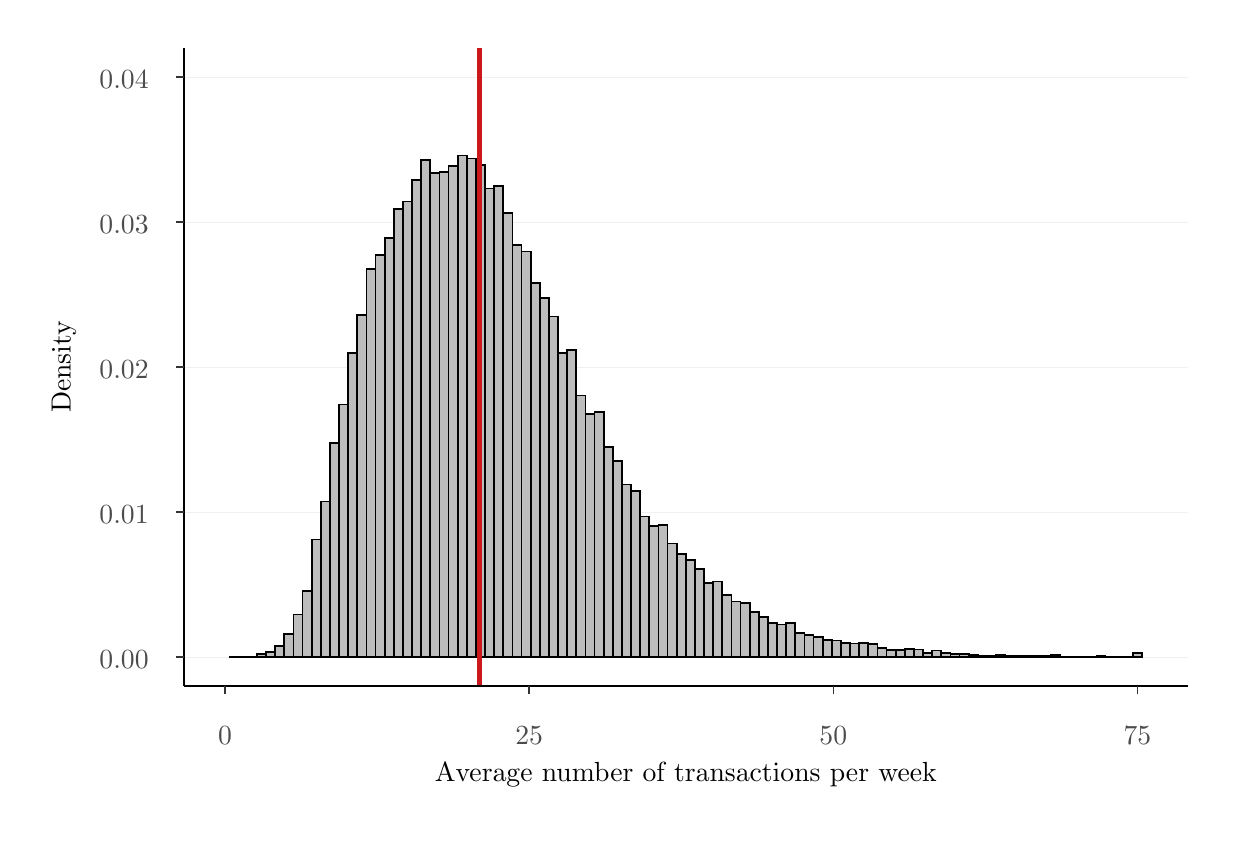
\begin{tikzpicture}[x=1pt,y=1pt]
\definecolor{fillColor}{RGB}{255,255,255}
\path[use as bounding box,fill=fillColor,fill opacity=0.00] (0,0) rectangle (433.62,289.08);
\begin{scope}
\path[clip] (  0.00,  0.00) rectangle (433.62,289.08);
\definecolor{drawColor}{RGB}{255,255,255}
\definecolor{fillColor}{RGB}{255,255,255}

\path[draw=drawColor,line width= 0.6pt,line join=round,line cap=round,fill=fillColor] ( -0.00,  0.00) rectangle (433.62,289.08);
\end{scope}
\begin{scope}
\path[clip] ( 56.47, 51.15) rectangle (419.17,281.85);
\definecolor{drawColor}{RGB}{255,255,255}

\path[draw=drawColor,line width= 0.3pt,line join=round] ( 56.47, 87.86) --
	(419.17, 87.86);

\path[draw=drawColor,line width= 0.3pt,line join=round] ( 56.47,140.29) --
	(419.17,140.29);

\path[draw=drawColor,line width= 0.3pt,line join=round] ( 56.47,192.72) --
	(419.17,192.72);

\path[draw=drawColor,line width= 0.3pt,line join=round] ( 56.47,245.15) --
	(419.17,245.15);

\path[draw=drawColor,line width= 0.3pt,line join=round] (126.26, 51.15) --
	(126.26,281.85);

\path[draw=drawColor,line width= 0.3pt,line join=round] (236.17, 51.15) --
	(236.17,281.85);

\path[draw=drawColor,line width= 0.3pt,line join=round] (346.08, 51.15) --
	(346.08,281.85);
\definecolor{drawColor}{gray}{0.94}

\path[draw=drawColor,line width= 0.1pt,line join=round] ( 56.47, 61.64) --
	(419.17, 61.64);

\path[draw=drawColor,line width= 0.1pt,line join=round] ( 56.47,114.07) --
	(419.17,114.07);

\path[draw=drawColor,line width= 0.1pt,line join=round] ( 56.47,166.50) --
	(419.17,166.50);

\path[draw=drawColor,line width= 0.1pt,line join=round] ( 56.47,218.93) --
	(419.17,218.93);

\path[draw=drawColor,line width= 0.1pt,line join=round] ( 56.47,271.37) --
	(419.17,271.37);
\definecolor{drawColor}{RGB}{0,0,0}
\definecolor{fillColor}{gray}{0.74}

\path[draw=drawColor,line width= 0.6pt,line cap=rect,fill=fillColor] ( 72.95, 61.64) rectangle ( 76.25, 61.71);

\path[draw=drawColor,line width= 0.6pt,line cap=rect,fill=fillColor] ( 76.25, 61.64) rectangle ( 79.55, 61.64);

\path[draw=drawColor,line width= 0.6pt,line cap=rect,fill=fillColor] ( 79.55, 61.64) rectangle ( 82.84, 61.79);

\path[draw=drawColor,line width= 0.6pt,line cap=rect,fill=fillColor] ( 82.84, 61.64) rectangle ( 86.14, 62.69);

\path[draw=drawColor,line width= 0.6pt,line cap=rect,fill=fillColor] ( 86.14, 61.64) rectangle ( 89.44, 63.43);

\path[draw=drawColor,line width= 0.6pt,line cap=rect,fill=fillColor] ( 89.44, 61.64) rectangle ( 92.74, 65.60);

\path[draw=drawColor,line width= 0.6pt,line cap=rect,fill=fillColor] ( 92.74, 61.64) rectangle ( 96.03, 69.94);

\path[draw=drawColor,line width= 0.6pt,line cap=rect,fill=fillColor] ( 96.03, 61.64) rectangle ( 99.33, 77.04);

\path[draw=drawColor,line width= 0.6pt,line cap=rect,fill=fillColor] ( 99.33, 61.64) rectangle (102.63, 85.56);

\path[draw=drawColor,line width= 0.6pt,line cap=rect,fill=fillColor] (102.63, 61.64) rectangle (105.92,104.17);

\path[draw=drawColor,line width= 0.6pt,line cap=rect,fill=fillColor] (105.92, 61.64) rectangle (109.22,117.92);

\path[draw=drawColor,line width= 0.6pt,line cap=rect,fill=fillColor] (109.22, 61.64) rectangle (112.52,138.92);

\path[draw=drawColor,line width= 0.6pt,line cap=rect,fill=fillColor] (112.52, 61.64) rectangle (115.82,152.97);

\path[draw=drawColor,line width= 0.6pt,line cap=rect,fill=fillColor] (115.82, 61.64) rectangle (119.11,171.51);

\path[draw=drawColor,line width= 0.6pt,line cap=rect,fill=fillColor] (119.11, 61.64) rectangle (122.41,185.19);

\path[draw=drawColor,line width= 0.6pt,line cap=rect,fill=fillColor] (122.41, 61.64) rectangle (125.71,201.85);

\path[draw=drawColor,line width= 0.6pt,line cap=rect,fill=fillColor] (125.71, 61.64) rectangle (129.01,206.94);

\path[draw=drawColor,line width= 0.6pt,line cap=rect,fill=fillColor] (129.01, 61.64) rectangle (132.30,213.14);

\path[draw=drawColor,line width= 0.6pt,line cap=rect,fill=fillColor] (132.30, 61.64) rectangle (135.60,223.53);

\path[draw=drawColor,line width= 0.6pt,line cap=rect,fill=fillColor] (135.60, 61.64) rectangle (138.90,226.22);

\path[draw=drawColor,line width= 0.6pt,line cap=rect,fill=fillColor] (138.90, 61.64) rectangle (142.19,234.07);

\path[draw=drawColor,line width= 0.6pt,line cap=rect,fill=fillColor] (142.19, 61.64) rectangle (145.49,241.17);

\path[draw=drawColor,line width= 0.6pt,line cap=rect,fill=fillColor] (145.49, 61.64) rectangle (148.79,236.46);

\path[draw=drawColor,line width= 0.6pt,line cap=rect,fill=fillColor] (148.79, 61.64) rectangle (152.09,236.98);

\path[draw=drawColor,line width= 0.6pt,line cap=rect,fill=fillColor] (152.09, 61.64) rectangle (155.38,239.08);

\path[draw=drawColor,line width= 0.6pt,line cap=rect,fill=fillColor] (155.38, 61.64) rectangle (158.68,242.89);

\path[draw=drawColor,line width= 0.6pt,line cap=rect,fill=fillColor] (158.68, 61.64) rectangle (161.98,241.77);

\path[draw=drawColor,line width= 0.6pt,line cap=rect,fill=fillColor] (161.98, 61.64) rectangle (165.28,239.45);

\path[draw=drawColor,line width= 0.6pt,line cap=rect,fill=fillColor] (165.28, 61.64) rectangle (168.57,231.00);

\path[draw=drawColor,line width= 0.6pt,line cap=rect,fill=fillColor] (168.57, 61.64) rectangle (171.87,231.98);

\path[draw=drawColor,line width= 0.6pt,line cap=rect,fill=fillColor] (171.87, 61.64) rectangle (175.17,222.03);

\path[draw=drawColor,line width= 0.6pt,line cap=rect,fill=fillColor] (175.17, 61.64) rectangle (178.46,210.45);

\path[draw=drawColor,line width= 0.6pt,line cap=rect,fill=fillColor] (178.46, 61.64) rectangle (181.76,208.21);

\path[draw=drawColor,line width= 0.6pt,line cap=rect,fill=fillColor] (181.76, 61.64) rectangle (185.06,196.85);

\path[draw=drawColor,line width= 0.6pt,line cap=rect,fill=fillColor] (185.06, 61.64) rectangle (188.36,191.39);

\path[draw=drawColor,line width= 0.6pt,line cap=rect,fill=fillColor] (188.36, 61.64) rectangle (191.65,184.74);

\path[draw=drawColor,line width= 0.6pt,line cap=rect,fill=fillColor] (191.65, 61.64) rectangle (194.95,171.58);

\path[draw=drawColor,line width= 0.6pt,line cap=rect,fill=fillColor] (194.95, 61.64) rectangle (198.25,172.56);

\path[draw=drawColor,line width= 0.6pt,line cap=rect,fill=fillColor] (198.25, 61.64) rectangle (201.55,156.19);

\path[draw=drawColor,line width= 0.6pt,line cap=rect,fill=fillColor] (201.55, 61.64) rectangle (204.84,149.39);

\path[draw=drawColor,line width= 0.6pt,line cap=rect,fill=fillColor] (204.84, 61.64) rectangle (208.14,150.21);

\path[draw=drawColor,line width= 0.6pt,line cap=rect,fill=fillColor] (208.14, 61.64) rectangle (211.44,137.65);

\path[draw=drawColor,line width= 0.6pt,line cap=rect,fill=fillColor] (211.44, 61.64) rectangle (214.73,132.42);

\path[draw=drawColor,line width= 0.6pt,line cap=rect,fill=fillColor] (214.73, 61.64) rectangle (218.03,123.97);

\path[draw=drawColor,line width= 0.6pt,line cap=rect,fill=fillColor] (218.03, 61.64) rectangle (221.33,121.73);

\path[draw=drawColor,line width= 0.6pt,line cap=rect,fill=fillColor] (221.33, 61.64) rectangle (224.63,112.39);

\path[draw=drawColor,line width= 0.6pt,line cap=rect,fill=fillColor] (224.63, 61.64) rectangle (227.92,109.10);

\path[draw=drawColor,line width= 0.6pt,line cap=rect,fill=fillColor] (227.92, 61.64) rectangle (231.22,109.47);

\path[draw=drawColor,line width= 0.6pt,line cap=rect,fill=fillColor] (231.22, 61.64) rectangle (234.52,102.67);

\path[draw=drawColor,line width= 0.6pt,line cap=rect,fill=fillColor] (234.52, 61.64) rectangle (237.82, 98.79);

\path[draw=drawColor,line width= 0.6pt,line cap=rect,fill=fillColor] (237.82, 61.64) rectangle (241.11, 96.84);

\path[draw=drawColor,line width= 0.6pt,line cap=rect,fill=fillColor] (241.11, 61.64) rectangle (244.41, 93.40);

\path[draw=drawColor,line width= 0.6pt,line cap=rect,fill=fillColor] (244.41, 61.64) rectangle (247.71, 88.47);

\path[draw=drawColor,line width= 0.6pt,line cap=rect,fill=fillColor] (247.71, 61.64) rectangle (251.00, 88.92);

\path[draw=drawColor,line width= 0.6pt,line cap=rect,fill=fillColor] (251.00, 61.64) rectangle (254.30, 83.99);

\path[draw=drawColor,line width= 0.6pt,line cap=rect,fill=fillColor] (254.30, 61.64) rectangle (257.60, 81.67);

\path[draw=drawColor,line width= 0.6pt,line cap=rect,fill=fillColor] (257.60, 61.64) rectangle (260.90, 81.15);

\path[draw=drawColor,line width= 0.6pt,line cap=rect,fill=fillColor] (260.90, 61.64) rectangle (264.19, 77.93);

\path[draw=drawColor,line width= 0.6pt,line cap=rect,fill=fillColor] (264.19, 61.64) rectangle (267.49, 76.06);

\path[draw=drawColor,line width= 0.6pt,line cap=rect,fill=fillColor] (267.49, 61.64) rectangle (270.79, 74.05);

\path[draw=drawColor,line width= 0.6pt,line cap=rect,fill=fillColor] (270.79, 61.64) rectangle (274.09, 73.37);

\path[draw=drawColor,line width= 0.6pt,line cap=rect,fill=fillColor] (274.09, 61.64) rectangle (277.38, 73.90);

\path[draw=drawColor,line width= 0.6pt,line cap=rect,fill=fillColor] (277.38, 61.64) rectangle (280.68, 70.24);

\path[draw=drawColor,line width= 0.6pt,line cap=rect,fill=fillColor] (280.68, 61.64) rectangle (283.98, 69.71);

\path[draw=drawColor,line width= 0.6pt,line cap=rect,fill=fillColor] (283.98, 61.64) rectangle (287.27, 68.89);

\path[draw=drawColor,line width= 0.6pt,line cap=rect,fill=fillColor] (287.27, 61.64) rectangle (290.57, 67.92);

\path[draw=drawColor,line width= 0.6pt,line cap=rect,fill=fillColor] (290.57, 61.64) rectangle (293.87, 67.69);

\path[draw=drawColor,line width= 0.6pt,line cap=rect,fill=fillColor] (293.87, 61.64) rectangle (297.17, 66.80);

\path[draw=drawColor,line width= 0.6pt,line cap=rect,fill=fillColor] (297.17, 61.64) rectangle (300.46, 66.57);

\path[draw=drawColor,line width= 0.6pt,line cap=rect,fill=fillColor] (300.46, 61.64) rectangle (303.76, 66.65);

\path[draw=drawColor,line width= 0.6pt,line cap=rect,fill=fillColor] (303.76, 61.64) rectangle (307.06, 66.42);

\path[draw=drawColor,line width= 0.6pt,line cap=rect,fill=fillColor] (307.06, 61.64) rectangle (310.36, 64.93);

\path[draw=drawColor,line width= 0.6pt,line cap=rect,fill=fillColor] (310.36, 61.64) rectangle (313.65, 64.11);

\path[draw=drawColor,line width= 0.6pt,line cap=rect,fill=fillColor] (313.65, 61.64) rectangle (316.95, 64.26);

\path[draw=drawColor,line width= 0.6pt,line cap=rect,fill=fillColor] (316.95, 61.64) rectangle (320.25, 64.55);

\path[draw=drawColor,line width= 0.6pt,line cap=rect,fill=fillColor] (320.25, 61.64) rectangle (323.55, 64.33);

\path[draw=drawColor,line width= 0.6pt,line cap=rect,fill=fillColor] (323.55, 61.64) rectangle (326.84, 63.21);

\path[draw=drawColor,line width= 0.6pt,line cap=rect,fill=fillColor] (326.84, 61.64) rectangle (330.14, 64.03);

\path[draw=drawColor,line width= 0.6pt,line cap=rect,fill=fillColor] (330.14, 61.64) rectangle (333.44, 63.21);

\path[draw=drawColor,line width= 0.6pt,line cap=rect,fill=fillColor] (333.44, 61.64) rectangle (336.73, 62.76);

\path[draw=drawColor,line width= 0.6pt,line cap=rect,fill=fillColor] (336.73, 61.64) rectangle (340.03, 62.69);

\path[draw=drawColor,line width= 0.6pt,line cap=rect,fill=fillColor] (340.03, 61.64) rectangle (343.33, 62.39);

\path[draw=drawColor,line width= 0.6pt,line cap=rect,fill=fillColor] (343.33, 61.64) rectangle (346.63, 62.16);

\path[draw=drawColor,line width= 0.6pt,line cap=rect,fill=fillColor] (346.63, 61.64) rectangle (349.92, 62.09);

\path[draw=drawColor,line width= 0.6pt,line cap=rect,fill=fillColor] (349.92, 61.64) rectangle (353.22, 62.46);

\path[draw=drawColor,line width= 0.6pt,line cap=rect,fill=fillColor] (353.22, 61.64) rectangle (356.52, 62.24);

\path[draw=drawColor,line width= 0.6pt,line cap=rect,fill=fillColor] (356.52, 61.64) rectangle (359.82, 62.24);

\path[draw=drawColor,line width= 0.6pt,line cap=rect,fill=fillColor] (359.82, 61.64) rectangle (363.11, 62.16);

\path[draw=drawColor,line width= 0.6pt,line cap=rect,fill=fillColor] (363.11, 61.64) rectangle (366.41, 61.94);

\path[draw=drawColor,line width= 0.6pt,line cap=rect,fill=fillColor] (366.41, 61.64) rectangle (369.71, 62.09);

\path[draw=drawColor,line width= 0.6pt,line cap=rect,fill=fillColor] (369.71, 61.64) rectangle (373.00, 62.46);

\path[draw=drawColor,line width= 0.6pt,line cap=rect,fill=fillColor] (373.00, 61.64) rectangle (376.30, 61.79);

\path[draw=drawColor,line width= 0.6pt,line cap=rect,fill=fillColor] (376.30, 61.64) rectangle (379.60, 61.86);

\path[draw=drawColor,line width= 0.6pt,line cap=rect,fill=fillColor] (379.60, 61.64) rectangle (382.90, 61.86);

\path[draw=drawColor,line width= 0.6pt,line cap=rect,fill=fillColor] (382.90, 61.64) rectangle (386.19, 61.86);

\path[draw=drawColor,line width= 0.6pt,line cap=rect,fill=fillColor] (386.19, 61.64) rectangle (389.49, 61.94);

\path[draw=drawColor,line width= 0.6pt,line cap=rect,fill=fillColor] (389.49, 61.64) rectangle (392.79, 61.79);

\path[draw=drawColor,line width= 0.6pt,line cap=rect,fill=fillColor] (392.79, 61.64) rectangle (396.09, 61.86);

\path[draw=drawColor,line width= 0.6pt,line cap=rect,fill=fillColor] (396.09, 61.64) rectangle (399.38, 61.79);

\path[draw=drawColor,line width= 0.6pt,line cap=rect,fill=fillColor] (399.38, 61.64) rectangle (402.68, 63.06);
\definecolor{drawColor}{RGB}{203,24,29}

\path[draw=drawColor,line width= 1.7pt,line join=round] (163.20, 51.15) -- (163.20,281.85);
\end{scope}
\begin{scope}
\path[clip] (  0.00,  0.00) rectangle (433.62,289.08);
\definecolor{drawColor}{RGB}{0,0,0}

\path[draw=drawColor,line width= 0.6pt,line join=round] ( 56.47, 51.15) --
	( 56.47,281.85);
\end{scope}
\begin{scope}
\path[clip] (  0.00,  0.00) rectangle (433.62,289.08);
\definecolor{drawColor}{gray}{0.30}

\node[text=drawColor,anchor=base east,inner sep=0pt, outer sep=0pt, scale=  1.00] at ( 43.72, 57.51) {0.00};

\node[text=drawColor,anchor=base east,inner sep=0pt, outer sep=0pt, scale=  1.00] at ( 43.72,109.94) {0.01};

\node[text=drawColor,anchor=base east,inner sep=0pt, outer sep=0pt, scale=  1.00] at ( 43.72,162.37) {0.02};

\node[text=drawColor,anchor=base east,inner sep=0pt, outer sep=0pt, scale=  1.00] at ( 43.72,214.80) {0.03};

\node[text=drawColor,anchor=base east,inner sep=0pt, outer sep=0pt, scale=  1.00] at ( 43.72,267.23) {0.04};
\end{scope}
\begin{scope}
\path[clip] (  0.00,  0.00) rectangle (433.62,289.08);
\definecolor{drawColor}{gray}{0.20}

\path[draw=drawColor,line width= 0.6pt,line join=round] ( 53.72, 61.64) --
	( 56.47, 61.64);

\path[draw=drawColor,line width= 0.6pt,line join=round] ( 53.72,114.07) --
	( 56.47,114.07);

\path[draw=drawColor,line width= 0.6pt,line join=round] ( 53.72,166.50) --
	( 56.47,166.50);

\path[draw=drawColor,line width= 0.6pt,line join=round] ( 53.72,218.93) --
	( 56.47,218.93);

\path[draw=drawColor,line width= 0.6pt,line join=round] ( 53.72,271.37) --
	( 56.47,271.37);
\end{scope}
\begin{scope}
\path[clip] (  0.00,  0.00) rectangle (433.62,289.08);
\definecolor{drawColor}{RGB}{0,0,0}

\path[draw=drawColor,line width= 0.6pt,line join=round] ( 56.47, 51.15) --
	(419.17, 51.15);
\end{scope}
\begin{scope}
\path[clip] (  0.00,  0.00) rectangle (433.62,289.08);
\definecolor{drawColor}{gray}{0.20}

\path[draw=drawColor,line width= 0.6pt,line join=round] ( 71.30, 48.40) --
	( 71.30, 51.15);

\path[draw=drawColor,line width= 0.6pt,line join=round] (181.21, 48.40) --
	(181.21, 51.15);

\path[draw=drawColor,line width= 0.6pt,line join=round] (291.12, 48.40) --
	(291.12, 51.15);

\path[draw=drawColor,line width= 0.6pt,line join=round] (401.03, 48.40) --
	(401.03, 51.15);
\end{scope}
\begin{scope}
\path[clip] (  0.00,  0.00) rectangle (433.62,289.08);
\definecolor{drawColor}{gray}{0.30}

\node[text=drawColor,anchor=base,inner sep=0pt, outer sep=0pt, scale=  1.00] at ( 71.30, 30.14) {0};

\node[text=drawColor,anchor=base,inner sep=0pt, outer sep=0pt, scale=  1.00] at (181.21, 30.14) {25};

\node[text=drawColor,anchor=base,inner sep=0pt, outer sep=0pt, scale=  1.00] at (291.12, 30.14) {50};

\node[text=drawColor,anchor=base,inner sep=0pt, outer sep=0pt, scale=  1.00] at (401.03, 30.14) {75};
\end{scope}
\begin{scope}
\path[clip] (  0.00,  0.00) rectangle (433.62,289.08);
\definecolor{drawColor}{RGB}{0,0,0}

\node[text=drawColor,anchor=base,inner sep=0pt, outer sep=0pt, scale=  1.00] at (237.82, 16.79) {Average number of transactions per week};
\end{scope}
\begin{scope}
\path[clip] (  0.00,  0.00) rectangle (433.62,289.08);
\definecolor{drawColor}{RGB}{0,0,0}

\node[text=drawColor,rotate= 90.00,anchor=base,inner sep=0pt, outer sep=0pt, scale=  1.00] at ( 15.49,166.50) {Density};
\end{scope}
\end{tikzpicture}
}
     \end{subfigure}\\
     \begin{subfigure}[t]{.49\textwidth}
         \centering
         \caption{Germany}
         \scalebox{0.45}{% Created by tikzDevice version 0.12.3.1 on 2022-07-29 15:13:42
% !TEX encoding = UTF-8 Unicode
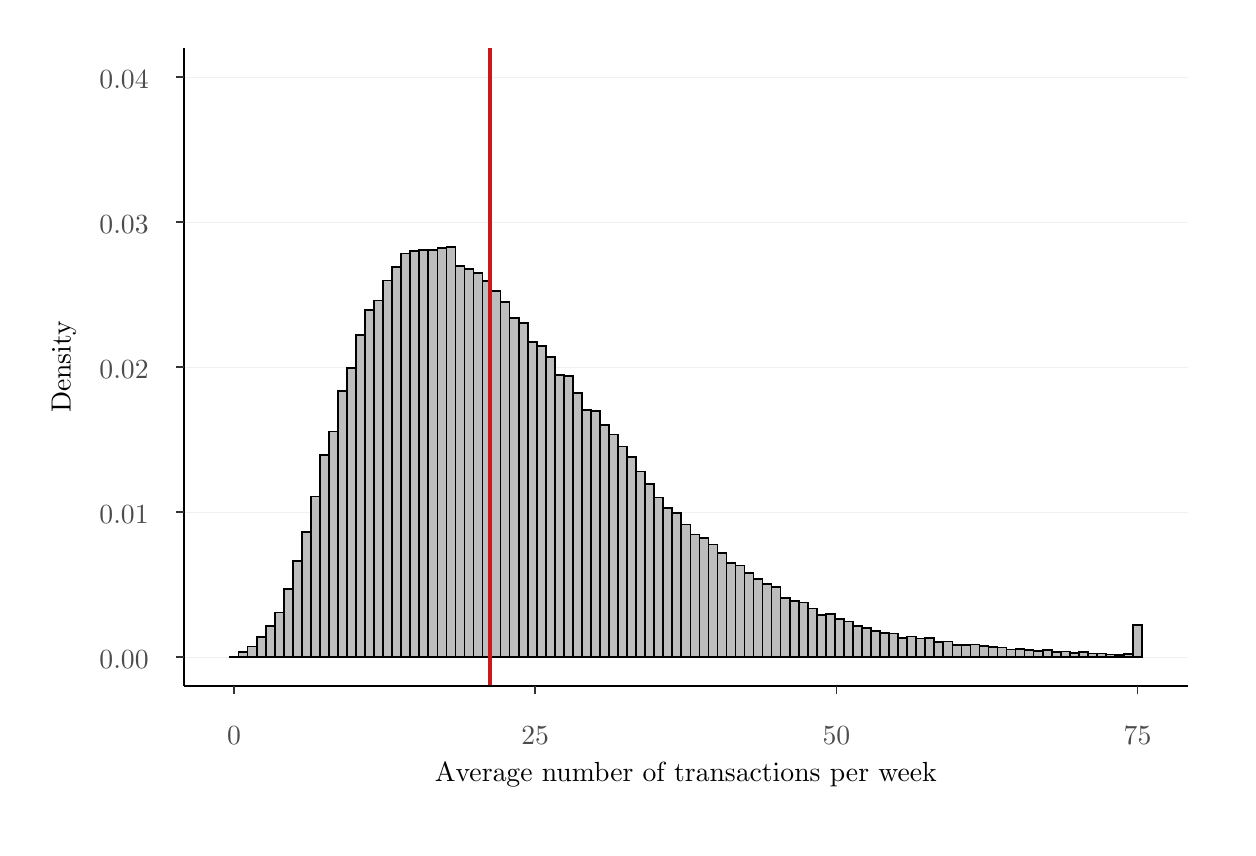
\begin{tikzpicture}[x=1pt,y=1pt]
\definecolor{fillColor}{RGB}{255,255,255}
\path[use as bounding box,fill=fillColor,fill opacity=0.00] (0,0) rectangle (433.62,289.08);
\begin{scope}
\path[clip] (  0.00,  0.00) rectangle (433.62,289.08);
\definecolor{drawColor}{RGB}{255,255,255}
\definecolor{fillColor}{RGB}{255,255,255}

\path[draw=drawColor,line width= 0.6pt,line join=round,line cap=round,fill=fillColor] ( -0.00,  0.00) rectangle (433.62,289.08);
\end{scope}
\begin{scope}
\path[clip] ( 56.47, 51.15) rectangle (419.17,281.85);
\definecolor{drawColor}{RGB}{255,255,255}

\path[draw=drawColor,line width= 0.3pt,line join=round] ( 56.47, 87.86) --
	(419.17, 87.86);

\path[draw=drawColor,line width= 0.3pt,line join=round] ( 56.47,140.29) --
	(419.17,140.29);

\path[draw=drawColor,line width= 0.3pt,line join=round] ( 56.47,192.72) --
	(419.17,192.72);

\path[draw=drawColor,line width= 0.3pt,line join=round] ( 56.47,245.15) --
	(419.17,245.15);

\path[draw=drawColor,line width= 0.3pt,line join=round] (128.99, 51.15) --
	(128.99,281.85);

\path[draw=drawColor,line width= 0.3pt,line join=round] (237.82, 51.15) --
	(237.82,281.85);

\path[draw=drawColor,line width= 0.3pt,line join=round] (346.64, 51.15) --
	(346.64,281.85);
\definecolor{drawColor}{gray}{0.94}

\path[draw=drawColor,line width= 0.1pt,line join=round] ( 56.47, 61.64) --
	(419.17, 61.64);

\path[draw=drawColor,line width= 0.1pt,line join=round] ( 56.47,114.07) --
	(419.17,114.07);

\path[draw=drawColor,line width= 0.1pt,line join=round] ( 56.47,166.50) --
	(419.17,166.50);

\path[draw=drawColor,line width= 0.1pt,line join=round] ( 56.47,218.93) --
	(419.17,218.93);

\path[draw=drawColor,line width= 0.1pt,line join=round] ( 56.47,271.37) --
	(419.17,271.37);
\definecolor{drawColor}{RGB}{0,0,0}
\definecolor{fillColor}{gray}{0.74}

\path[draw=drawColor,line width= 0.6pt,line cap=rect,fill=fillColor] ( 72.95, 61.64) rectangle ( 76.22, 61.77);

\path[draw=drawColor,line width= 0.6pt,line cap=rect,fill=fillColor] ( 76.22, 61.64) rectangle ( 79.48, 63.57);

\path[draw=drawColor,line width= 0.6pt,line cap=rect,fill=fillColor] ( 79.48, 61.64) rectangle ( 82.75, 65.41);

\path[draw=drawColor,line width= 0.6pt,line cap=rect,fill=fillColor] ( 82.75, 61.64) rectangle ( 86.01, 68.85);

\path[draw=drawColor,line width= 0.6pt,line cap=rect,fill=fillColor] ( 86.01, 61.64) rectangle ( 89.28, 72.85);

\path[draw=drawColor,line width= 0.6pt,line cap=rect,fill=fillColor] ( 89.28, 61.64) rectangle ( 92.54, 77.79);

\path[draw=drawColor,line width= 0.6pt,line cap=rect,fill=fillColor] ( 92.54, 61.64) rectangle ( 95.80, 86.32);

\path[draw=drawColor,line width= 0.6pt,line cap=rect,fill=fillColor] ( 95.80, 61.64) rectangle ( 99.07, 96.36);

\path[draw=drawColor,line width= 0.6pt,line cap=rect,fill=fillColor] ( 99.07, 61.64) rectangle (102.33,106.80);

\path[draw=drawColor,line width= 0.6pt,line cap=rect,fill=fillColor] (102.33, 61.64) rectangle (105.60,119.69);

\path[draw=drawColor,line width= 0.6pt,line cap=rect,fill=fillColor] (105.60, 61.64) rectangle (108.86,134.62);

\path[draw=drawColor,line width= 0.6pt,line cap=rect,fill=fillColor] (108.86, 61.64) rectangle (112.13,143.11);

\path[draw=drawColor,line width= 0.6pt,line cap=rect,fill=fillColor] (112.13, 61.64) rectangle (115.39,157.80);

\path[draw=drawColor,line width= 0.6pt,line cap=rect,fill=fillColor] (115.39, 61.64) rectangle (118.66,166.06);

\path[draw=drawColor,line width= 0.6pt,line cap=rect,fill=fillColor] (118.66, 61.64) rectangle (121.92,178.05);

\path[draw=drawColor,line width= 0.6pt,line cap=rect,fill=fillColor] (121.92, 61.64) rectangle (125.19,187.15);

\path[draw=drawColor,line width= 0.6pt,line cap=rect,fill=fillColor] (125.19, 61.64) rectangle (128.45,190.50);

\path[draw=drawColor,line width= 0.6pt,line cap=rect,fill=fillColor] (128.45, 61.64) rectangle (131.72,197.77);

\path[draw=drawColor,line width= 0.6pt,line cap=rect,fill=fillColor] (131.72, 61.64) rectangle (134.98,202.62);

\path[draw=drawColor,line width= 0.6pt,line cap=rect,fill=fillColor] (134.98, 61.64) rectangle (138.24,207.43);

\path[draw=drawColor,line width= 0.6pt,line cap=rect,fill=fillColor] (138.24, 61.64) rectangle (141.51,208.37);

\path[draw=drawColor,line width= 0.6pt,line cap=rect,fill=fillColor] (141.51, 61.64) rectangle (144.77,208.78);

\path[draw=drawColor,line width= 0.6pt,line cap=rect,fill=fillColor] (144.77, 61.64) rectangle (148.04,208.62);

\path[draw=drawColor,line width= 0.6pt,line cap=rect,fill=fillColor] (148.04, 61.64) rectangle (151.30,209.47);

\path[draw=drawColor,line width= 0.6pt,line cap=rect,fill=fillColor] (151.30, 61.64) rectangle (154.57,209.94);

\path[draw=drawColor,line width= 0.6pt,line cap=rect,fill=fillColor] (154.57, 61.64) rectangle (157.83,202.85);

\path[draw=drawColor,line width= 0.6pt,line cap=rect,fill=fillColor] (157.83, 61.64) rectangle (161.10,201.95);

\path[draw=drawColor,line width= 0.6pt,line cap=rect,fill=fillColor] (161.10, 61.64) rectangle (164.36,200.31);

\path[draw=drawColor,line width= 0.6pt,line cap=rect,fill=fillColor] (164.36, 61.64) rectangle (167.63,197.55);

\path[draw=drawColor,line width= 0.6pt,line cap=rect,fill=fillColor] (167.63, 61.64) rectangle (170.89,193.82);

\path[draw=drawColor,line width= 0.6pt,line cap=rect,fill=fillColor] (170.89, 61.64) rectangle (174.16,189.93);

\path[draw=drawColor,line width= 0.6pt,line cap=rect,fill=fillColor] (174.16, 61.64) rectangle (177.42,184.25);

\path[draw=drawColor,line width= 0.6pt,line cap=rect,fill=fillColor] (177.42, 61.64) rectangle (180.68,182.32);

\path[draw=drawColor,line width= 0.6pt,line cap=rect,fill=fillColor] (180.68, 61.64) rectangle (183.95,175.56);

\path[draw=drawColor,line width= 0.6pt,line cap=rect,fill=fillColor] (183.95, 61.64) rectangle (187.21,173.99);

\path[draw=drawColor,line width= 0.6pt,line cap=rect,fill=fillColor] (187.21, 61.64) rectangle (190.48,170.02);

\path[draw=drawColor,line width= 0.6pt,line cap=rect,fill=fillColor] (190.48, 61.64) rectangle (193.74,163.64);

\path[draw=drawColor,line width= 0.6pt,line cap=rect,fill=fillColor] (193.74, 61.64) rectangle (197.01,163.30);

\path[draw=drawColor,line width= 0.6pt,line cap=rect,fill=fillColor] (197.01, 61.64) rectangle (200.27,157.15);

\path[draw=drawColor,line width= 0.6pt,line cap=rect,fill=fillColor] (200.27, 61.64) rectangle (203.54,150.97);

\path[draw=drawColor,line width= 0.6pt,line cap=rect,fill=fillColor] (203.54, 61.64) rectangle (206.80,150.50);

\path[draw=drawColor,line width= 0.6pt,line cap=rect,fill=fillColor] (206.80, 61.64) rectangle (210.07,145.54);

\path[draw=drawColor,line width= 0.6pt,line cap=rect,fill=fillColor] (210.07, 61.64) rectangle (213.33,142.06);

\path[draw=drawColor,line width= 0.6pt,line cap=rect,fill=fillColor] (213.33, 61.64) rectangle (216.60,137.75);

\path[draw=drawColor,line width= 0.6pt,line cap=rect,fill=fillColor] (216.60, 61.64) rectangle (219.86,134.04);

\path[draw=drawColor,line width= 0.6pt,line cap=rect,fill=fillColor] (219.86, 61.64) rectangle (223.13,128.67);

\path[draw=drawColor,line width= 0.6pt,line cap=rect,fill=fillColor] (223.13, 61.64) rectangle (226.39,124.25);

\path[draw=drawColor,line width= 0.6pt,line cap=rect,fill=fillColor] (226.39, 61.64) rectangle (229.65,119.26);

\path[draw=drawColor,line width= 0.6pt,line cap=rect,fill=fillColor] (229.65, 61.64) rectangle (232.92,115.49);

\path[draw=drawColor,line width= 0.6pt,line cap=rect,fill=fillColor] (232.92, 61.64) rectangle (236.18,113.72);

\path[draw=drawColor,line width= 0.6pt,line cap=rect,fill=fillColor] (236.18, 61.64) rectangle (239.45,109.49);

\path[draw=drawColor,line width= 0.6pt,line cap=rect,fill=fillColor] (239.45, 61.64) rectangle (242.71,105.92);

\path[draw=drawColor,line width= 0.6pt,line cap=rect,fill=fillColor] (242.71, 61.64) rectangle (245.98,104.64);

\path[draw=drawColor,line width= 0.6pt,line cap=rect,fill=fillColor] (245.98, 61.64) rectangle (249.24,102.38);

\path[draw=drawColor,line width= 0.6pt,line cap=rect,fill=fillColor] (249.24, 61.64) rectangle (252.51, 99.19);

\path[draw=drawColor,line width= 0.6pt,line cap=rect,fill=fillColor] (252.51, 61.64) rectangle (255.77, 95.64);

\path[draw=drawColor,line width= 0.6pt,line cap=rect,fill=fillColor] (255.77, 61.64) rectangle (259.04, 94.79);

\path[draw=drawColor,line width= 0.6pt,line cap=rect,fill=fillColor] (259.04, 61.64) rectangle (262.30, 92.11);

\path[draw=drawColor,line width= 0.6pt,line cap=rect,fill=fillColor] (262.30, 61.64) rectangle (265.57, 89.80);

\path[draw=drawColor,line width= 0.6pt,line cap=rect,fill=fillColor] (265.57, 61.64) rectangle (268.83, 88.09);

\path[draw=drawColor,line width= 0.6pt,line cap=rect,fill=fillColor] (268.83, 61.64) rectangle (272.09, 87.04);

\path[draw=drawColor,line width= 0.6pt,line cap=rect,fill=fillColor] (272.09, 61.64) rectangle (275.36, 83.11);

\path[draw=drawColor,line width= 0.6pt,line cap=rect,fill=fillColor] (275.36, 61.64) rectangle (278.62, 81.85);

\path[draw=drawColor,line width= 0.6pt,line cap=rect,fill=fillColor] (278.62, 61.64) rectangle (281.89, 81.42);

\path[draw=drawColor,line width= 0.6pt,line cap=rect,fill=fillColor] (281.89, 61.64) rectangle (285.15, 79.18);

\path[draw=drawColor,line width= 0.6pt,line cap=rect,fill=fillColor] (285.15, 61.64) rectangle (288.42, 76.93);

\path[draw=drawColor,line width= 0.6pt,line cap=rect,fill=fillColor] (288.42, 61.64) rectangle (291.68, 77.18);

\path[draw=drawColor,line width= 0.6pt,line cap=rect,fill=fillColor] (291.68, 61.64) rectangle (294.95, 75.32);

\path[draw=drawColor,line width= 0.6pt,line cap=rect,fill=fillColor] (294.95, 61.64) rectangle (298.21, 74.53);

\path[draw=drawColor,line width= 0.6pt,line cap=rect,fill=fillColor] (298.21, 61.64) rectangle (301.48, 72.87);

\path[draw=drawColor,line width= 0.6pt,line cap=rect,fill=fillColor] (301.48, 61.64) rectangle (304.74, 72.19);

\path[draw=drawColor,line width= 0.6pt,line cap=rect,fill=fillColor] (304.74, 61.64) rectangle (308.01, 71.18);

\path[draw=drawColor,line width= 0.6pt,line cap=rect,fill=fillColor] (308.01, 61.64) rectangle (311.27, 70.24);

\path[draw=drawColor,line width= 0.6pt,line cap=rect,fill=fillColor] (311.27, 61.64) rectangle (314.53, 70.15);

\path[draw=drawColor,line width= 0.6pt,line cap=rect,fill=fillColor] (314.53, 61.64) rectangle (317.80, 68.51);

\path[draw=drawColor,line width= 0.6pt,line cap=rect,fill=fillColor] (317.80, 61.64) rectangle (321.06, 69.12);

\path[draw=drawColor,line width= 0.6pt,line cap=rect,fill=fillColor] (321.06, 61.64) rectangle (324.33, 68.33);

\path[draw=drawColor,line width= 0.6pt,line cap=rect,fill=fillColor] (324.33, 61.64) rectangle (327.59, 68.56);

\path[draw=drawColor,line width= 0.6pt,line cap=rect,fill=fillColor] (327.59, 61.64) rectangle (330.86, 66.98);

\path[draw=drawColor,line width= 0.6pt,line cap=rect,fill=fillColor] (330.86, 61.64) rectangle (334.12, 67.25);

\path[draw=drawColor,line width= 0.6pt,line cap=rect,fill=fillColor] (334.12, 61.64) rectangle (337.39, 66.09);

\path[draw=drawColor,line width= 0.6pt,line cap=rect,fill=fillColor] (337.39, 61.64) rectangle (340.65, 66.06);

\path[draw=drawColor,line width= 0.6pt,line cap=rect,fill=fillColor] (340.65, 61.64) rectangle (343.92, 66.13);

\path[draw=drawColor,line width= 0.6pt,line cap=rect,fill=fillColor] (343.92, 61.64) rectangle (347.18, 65.75);

\path[draw=drawColor,line width= 0.6pt,line cap=rect,fill=fillColor] (347.18, 61.64) rectangle (350.45, 65.26);

\path[draw=drawColor,line width= 0.6pt,line cap=rect,fill=fillColor] (350.45, 61.64) rectangle (353.71, 65.10);

\path[draw=drawColor,line width= 0.6pt,line cap=rect,fill=fillColor] (353.71, 61.64) rectangle (356.97, 64.36);

\path[draw=drawColor,line width= 0.6pt,line cap=rect,fill=fillColor] (356.97, 61.64) rectangle (360.24, 64.49);

\path[draw=drawColor,line width= 0.6pt,line cap=rect,fill=fillColor] (360.24, 61.64) rectangle (363.50, 64.27);

\path[draw=drawColor,line width= 0.6pt,line cap=rect,fill=fillColor] (363.50, 61.64) rectangle (366.77, 63.86);

\path[draw=drawColor,line width= 0.6pt,line cap=rect,fill=fillColor] (366.77, 61.64) rectangle (370.03, 64.11);

\path[draw=drawColor,line width= 0.6pt,line cap=rect,fill=fillColor] (370.03, 61.64) rectangle (373.30, 63.55);

\path[draw=drawColor,line width= 0.6pt,line cap=rect,fill=fillColor] (373.30, 61.64) rectangle (376.56, 63.68);

\path[draw=drawColor,line width= 0.6pt,line cap=rect,fill=fillColor] (376.56, 61.64) rectangle (379.83, 63.21);

\path[draw=drawColor,line width= 0.6pt,line cap=rect,fill=fillColor] (379.83, 61.64) rectangle (383.09, 63.37);

\path[draw=drawColor,line width= 0.6pt,line cap=rect,fill=fillColor] (383.09, 61.64) rectangle (386.36, 62.99);

\path[draw=drawColor,line width= 0.6pt,line cap=rect,fill=fillColor] (386.36, 61.64) rectangle (389.62, 62.88);

\path[draw=drawColor,line width= 0.6pt,line cap=rect,fill=fillColor] (389.62, 61.64) rectangle (392.89, 62.63);

\path[draw=drawColor,line width= 0.6pt,line cap=rect,fill=fillColor] (392.89, 61.64) rectangle (396.15, 62.47);

\path[draw=drawColor,line width= 0.6pt,line cap=rect,fill=fillColor] (396.15, 61.64) rectangle (399.41, 62.65);

\path[draw=drawColor,line width= 0.6pt,line cap=rect,fill=fillColor] (399.41, 61.64) rectangle (402.68, 73.29);
\definecolor{drawColor}{RGB}{203,24,29}

\path[draw=drawColor,line width= 1.7pt,line join=round] (167.08, 51.15) -- (167.08,281.85);
\end{scope}
\begin{scope}
\path[clip] (  0.00,  0.00) rectangle (433.62,289.08);
\definecolor{drawColor}{RGB}{0,0,0}

\path[draw=drawColor,line width= 0.6pt,line join=round] ( 56.47, 51.15) --
	( 56.47,281.85);
\end{scope}
\begin{scope}
\path[clip] (  0.00,  0.00) rectangle (433.62,289.08);
\definecolor{drawColor}{gray}{0.30}

\node[text=drawColor,anchor=base east,inner sep=0pt, outer sep=0pt, scale=  1.00] at ( 43.72, 57.51) {0.00};

\node[text=drawColor,anchor=base east,inner sep=0pt, outer sep=0pt, scale=  1.00] at ( 43.72,109.94) {0.01};

\node[text=drawColor,anchor=base east,inner sep=0pt, outer sep=0pt, scale=  1.00] at ( 43.72,162.37) {0.02};

\node[text=drawColor,anchor=base east,inner sep=0pt, outer sep=0pt, scale=  1.00] at ( 43.72,214.80) {0.03};

\node[text=drawColor,anchor=base east,inner sep=0pt, outer sep=0pt, scale=  1.00] at ( 43.72,267.23) {0.04};
\end{scope}
\begin{scope}
\path[clip] (  0.00,  0.00) rectangle (433.62,289.08);
\definecolor{drawColor}{gray}{0.20}

\path[draw=drawColor,line width= 0.6pt,line join=round] ( 53.72, 61.64) --
	( 56.47, 61.64);

\path[draw=drawColor,line width= 0.6pt,line join=round] ( 53.72,114.07) --
	( 56.47,114.07);

\path[draw=drawColor,line width= 0.6pt,line join=round] ( 53.72,166.50) --
	( 56.47,166.50);

\path[draw=drawColor,line width= 0.6pt,line join=round] ( 53.72,218.93) --
	( 56.47,218.93);

\path[draw=drawColor,line width= 0.6pt,line join=round] ( 53.72,271.37) --
	( 56.47,271.37);
\end{scope}
\begin{scope}
\path[clip] (  0.00,  0.00) rectangle (433.62,289.08);
\definecolor{drawColor}{RGB}{0,0,0}

\path[draw=drawColor,line width= 0.6pt,line join=round] ( 56.47, 51.15) --
	(419.17, 51.15);
\end{scope}
\begin{scope}
\path[clip] (  0.00,  0.00) rectangle (433.62,289.08);
\definecolor{drawColor}{gray}{0.20}

\path[draw=drawColor,line width= 0.6pt,line join=round] ( 74.58, 48.40) --
	( 74.58, 51.15);

\path[draw=drawColor,line width= 0.6pt,line join=round] (183.41, 48.40) --
	(183.41, 51.15);

\path[draw=drawColor,line width= 0.6pt,line join=round] (292.23, 48.40) --
	(292.23, 51.15);

\path[draw=drawColor,line width= 0.6pt,line join=round] (401.05, 48.40) --
	(401.05, 51.15);
\end{scope}
\begin{scope}
\path[clip] (  0.00,  0.00) rectangle (433.62,289.08);
\definecolor{drawColor}{gray}{0.30}

\node[text=drawColor,anchor=base,inner sep=0pt, outer sep=0pt, scale=  1.00] at ( 74.58, 30.14) {0};

\node[text=drawColor,anchor=base,inner sep=0pt, outer sep=0pt, scale=  1.00] at (183.41, 30.14) {25};

\node[text=drawColor,anchor=base,inner sep=0pt, outer sep=0pt, scale=  1.00] at (292.23, 30.14) {50};

\node[text=drawColor,anchor=base,inner sep=0pt, outer sep=0pt, scale=  1.00] at (401.05, 30.14) {75};
\end{scope}
\begin{scope}
\path[clip] (  0.00,  0.00) rectangle (433.62,289.08);
\definecolor{drawColor}{RGB}{0,0,0}

\node[text=drawColor,anchor=base,inner sep=0pt, outer sep=0pt, scale=  1.00] at (237.82, 16.79) {Average number of transactions per week};
\end{scope}
\begin{scope}
\path[clip] (  0.00,  0.00) rectangle (433.62,289.08);
\definecolor{drawColor}{RGB}{0,0,0}

\node[text=drawColor,rotate= 90.00,anchor=base,inner sep=0pt, outer sep=0pt, scale=  1.00] at ( 15.49,166.50) {Density};
\end{scope}
\end{tikzpicture}
}
     \end{subfigure}
     \begin{subfigure}[t]{.49\textwidth}
         \centering
         \caption{The Netherlands}
         \scalebox{0.45}{% Created by tikzDevice version 0.12.3.1 on 2022-07-29 15:13:42
% !TEX encoding = UTF-8 Unicode
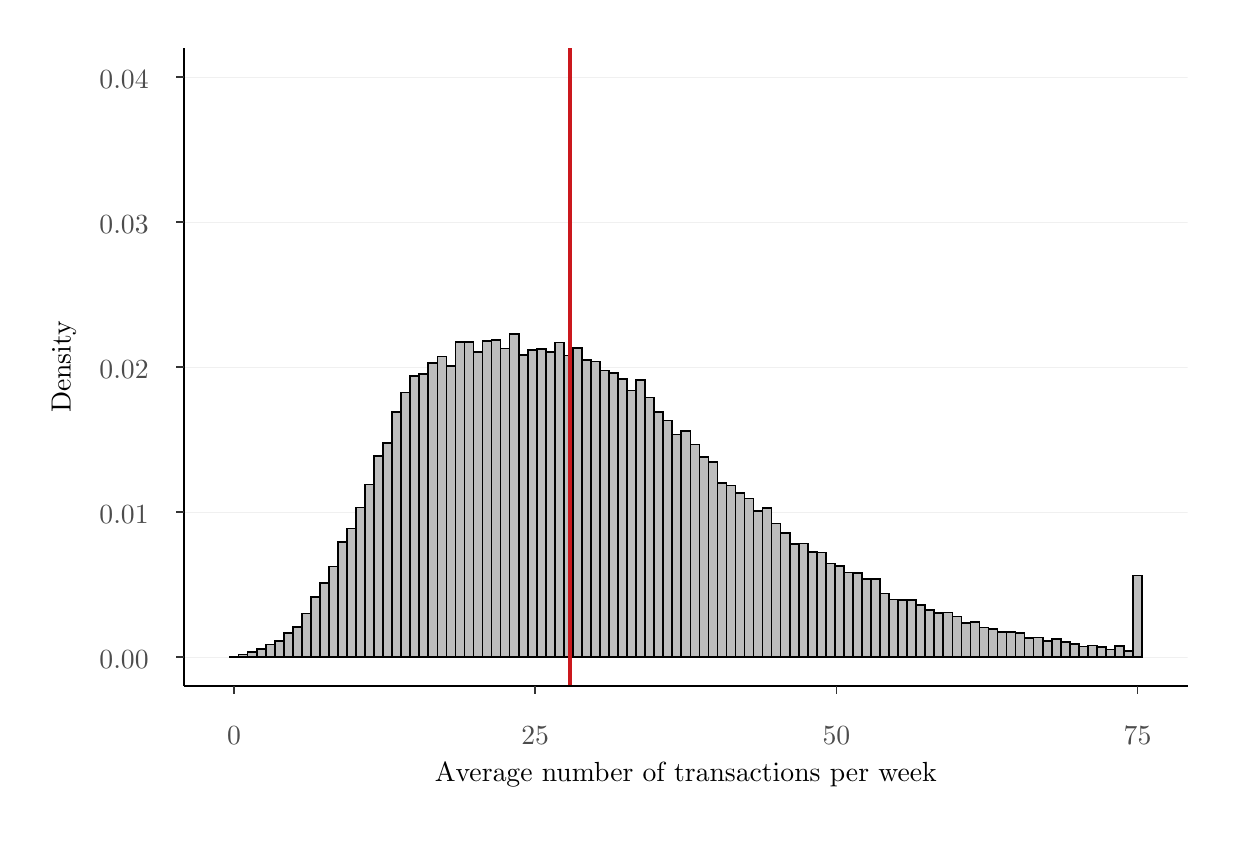
\begin{tikzpicture}[x=1pt,y=1pt]
\definecolor{fillColor}{RGB}{255,255,255}
\path[use as bounding box,fill=fillColor,fill opacity=0.00] (0,0) rectangle (433.62,289.08);
\begin{scope}
\path[clip] (  0.00,  0.00) rectangle (433.62,289.08);
\definecolor{drawColor}{RGB}{255,255,255}
\definecolor{fillColor}{RGB}{255,255,255}

\path[draw=drawColor,line width= 0.6pt,line join=round,line cap=round,fill=fillColor] ( -0.00,  0.00) rectangle (433.62,289.08);
\end{scope}
\begin{scope}
\path[clip] ( 56.47, 51.15) rectangle (419.17,281.85);
\definecolor{drawColor}{RGB}{255,255,255}

\path[draw=drawColor,line width= 0.3pt,line join=round] ( 56.47, 87.86) --
	(419.17, 87.86);

\path[draw=drawColor,line width= 0.3pt,line join=round] ( 56.47,140.29) --
	(419.17,140.29);

\path[draw=drawColor,line width= 0.3pt,line join=round] ( 56.47,192.72) --
	(419.17,192.72);

\path[draw=drawColor,line width= 0.3pt,line join=round] ( 56.47,245.15) --
	(419.17,245.15);

\path[draw=drawColor,line width= 0.3pt,line join=round] (128.99, 51.15) --
	(128.99,281.85);

\path[draw=drawColor,line width= 0.3pt,line join=round] (237.82, 51.15) --
	(237.82,281.85);

\path[draw=drawColor,line width= 0.3pt,line join=round] (346.64, 51.15) --
	(346.64,281.85);
\definecolor{drawColor}{gray}{0.94}

\path[draw=drawColor,line width= 0.1pt,line join=round] ( 56.47, 61.64) --
	(419.17, 61.64);

\path[draw=drawColor,line width= 0.1pt,line join=round] ( 56.47,114.07) --
	(419.17,114.07);

\path[draw=drawColor,line width= 0.1pt,line join=round] ( 56.47,166.50) --
	(419.17,166.50);

\path[draw=drawColor,line width= 0.1pt,line join=round] ( 56.47,218.93) --
	(419.17,218.93);

\path[draw=drawColor,line width= 0.1pt,line join=round] ( 56.47,271.37) --
	(419.17,271.37);
\definecolor{drawColor}{RGB}{0,0,0}
\definecolor{fillColor}{gray}{0.74}

\path[draw=drawColor,line width= 0.6pt,line cap=rect,fill=fillColor] ( 72.95, 61.64) rectangle ( 76.22, 61.83);

\path[draw=drawColor,line width= 0.6pt,line cap=rect,fill=fillColor] ( 76.22, 61.64) rectangle ( 79.48, 62.57);

\path[draw=drawColor,line width= 0.6pt,line cap=rect,fill=fillColor] ( 79.48, 61.64) rectangle ( 82.75, 63.50);

\path[draw=drawColor,line width= 0.6pt,line cap=rect,fill=fillColor] ( 82.75, 61.64) rectangle ( 86.01, 64.55);

\path[draw=drawColor,line width= 0.6pt,line cap=rect,fill=fillColor] ( 86.01, 61.64) rectangle ( 89.28, 66.16);

\path[draw=drawColor,line width= 0.6pt,line cap=rect,fill=fillColor] ( 89.28, 61.64) rectangle ( 92.54, 67.46);

\path[draw=drawColor,line width= 0.6pt,line cap=rect,fill=fillColor] ( 92.54, 61.64) rectangle ( 95.80, 70.31);

\path[draw=drawColor,line width= 0.6pt,line cap=rect,fill=fillColor] ( 95.80, 61.64) rectangle ( 99.07, 72.54);

\path[draw=drawColor,line width= 0.6pt,line cap=rect,fill=fillColor] ( 99.07, 61.64) rectangle (102.33, 77.43);

\path[draw=drawColor,line width= 0.6pt,line cap=rect,fill=fillColor] (102.33, 61.64) rectangle (105.60, 83.25);

\path[draw=drawColor,line width= 0.6pt,line cap=rect,fill=fillColor] (105.60, 61.64) rectangle (108.86, 88.51);

\path[draw=drawColor,line width= 0.6pt,line cap=rect,fill=fillColor] (108.86, 61.64) rectangle (112.13, 94.33);

\path[draw=drawColor,line width= 0.6pt,line cap=rect,fill=fillColor] (112.13, 61.64) rectangle (115.39,103.25);

\path[draw=drawColor,line width= 0.6pt,line cap=rect,fill=fillColor] (115.39, 61.64) rectangle (118.66,108.14);

\path[draw=drawColor,line width= 0.6pt,line cap=rect,fill=fillColor] (118.66, 61.64) rectangle (121.92,115.70);

\path[draw=drawColor,line width= 0.6pt,line cap=rect,fill=fillColor] (121.92, 61.64) rectangle (125.19,124.05);

\path[draw=drawColor,line width= 0.6pt,line cap=rect,fill=fillColor] (125.19, 61.64) rectangle (128.45,134.21);

\path[draw=drawColor,line width= 0.6pt,line cap=rect,fill=fillColor] (128.45, 61.64) rectangle (131.72,138.98);

\path[draw=drawColor,line width= 0.6pt,line cap=rect,fill=fillColor] (131.72, 61.64) rectangle (134.98,150.12);

\path[draw=drawColor,line width= 0.6pt,line cap=rect,fill=fillColor] (134.98, 61.64) rectangle (138.24,157.24);

\path[draw=drawColor,line width= 0.6pt,line cap=rect,fill=fillColor] (138.24, 61.64) rectangle (141.51,163.25);

\path[draw=drawColor,line width= 0.6pt,line cap=rect,fill=fillColor] (141.51, 61.64) rectangle (144.77,163.93);

\path[draw=drawColor,line width= 0.6pt,line cap=rect,fill=fillColor] (144.77, 61.64) rectangle (148.04,167.89);

\path[draw=drawColor,line width= 0.6pt,line cap=rect,fill=fillColor] (148.04, 61.64) rectangle (151.30,170.31);

\path[draw=drawColor,line width= 0.6pt,line cap=rect,fill=fillColor] (151.30, 61.64) rectangle (154.57,166.78);

\path[draw=drawColor,line width= 0.6pt,line cap=rect,fill=fillColor] (154.57, 61.64) rectangle (157.83,175.45);

\path[draw=drawColor,line width= 0.6pt,line cap=rect,fill=fillColor] (157.83, 61.64) rectangle (161.10,175.38);

\path[draw=drawColor,line width= 0.6pt,line cap=rect,fill=fillColor] (161.10, 61.64) rectangle (164.36,171.98);

\path[draw=drawColor,line width= 0.6pt,line cap=rect,fill=fillColor] (164.36, 61.64) rectangle (167.63,175.88);

\path[draw=drawColor,line width= 0.6pt,line cap=rect,fill=fillColor] (167.63, 61.64) rectangle (170.89,176.25);

\path[draw=drawColor,line width= 0.6pt,line cap=rect,fill=fillColor] (170.89, 61.64) rectangle (174.16,173.09);

\path[draw=drawColor,line width= 0.6pt,line cap=rect,fill=fillColor] (174.16, 61.64) rectangle (177.42,178.42);

\path[draw=drawColor,line width= 0.6pt,line cap=rect,fill=fillColor] (177.42, 61.64) rectangle (180.68,170.86);

\path[draw=drawColor,line width= 0.6pt,line cap=rect,fill=fillColor] (180.68, 61.64) rectangle (183.95,172.66);

\path[draw=drawColor,line width= 0.6pt,line cap=rect,fill=fillColor] (183.95, 61.64) rectangle (187.21,172.97);

\path[draw=drawColor,line width= 0.6pt,line cap=rect,fill=fillColor] (187.21, 61.64) rectangle (190.48,171.92);

\path[draw=drawColor,line width= 0.6pt,line cap=rect,fill=fillColor] (190.48, 61.64) rectangle (193.74,175.26);

\path[draw=drawColor,line width= 0.6pt,line cap=rect,fill=fillColor] (193.74, 61.64) rectangle (197.01,170.62);

\path[draw=drawColor,line width= 0.6pt,line cap=rect,fill=fillColor] (197.01, 61.64) rectangle (200.27,173.40);

\path[draw=drawColor,line width= 0.6pt,line cap=rect,fill=fillColor] (200.27, 61.64) rectangle (203.54,168.88);

\path[draw=drawColor,line width= 0.6pt,line cap=rect,fill=fillColor] (203.54, 61.64) rectangle (206.80,168.45);

\path[draw=drawColor,line width= 0.6pt,line cap=rect,fill=fillColor] (206.80, 61.64) rectangle (210.07,165.17);

\path[draw=drawColor,line width= 0.6pt,line cap=rect,fill=fillColor] (210.07, 61.64) rectangle (213.33,164.36);

\path[draw=drawColor,line width= 0.6pt,line cap=rect,fill=fillColor] (213.33, 61.64) rectangle (216.60,162.07);

\path[draw=drawColor,line width= 0.6pt,line cap=rect,fill=fillColor] (216.60, 61.64) rectangle (219.86,157.92);

\path[draw=drawColor,line width= 0.6pt,line cap=rect,fill=fillColor] (219.86, 61.64) rectangle (223.13,161.76);

\path[draw=drawColor,line width= 0.6pt,line cap=rect,fill=fillColor] (223.13, 61.64) rectangle (226.39,155.39);

\path[draw=drawColor,line width= 0.6pt,line cap=rect,fill=fillColor] (226.39, 61.64) rectangle (229.65,150.31);

\path[draw=drawColor,line width= 0.6pt,line cap=rect,fill=fillColor] (229.65, 61.64) rectangle (232.92,147.09);

\path[draw=drawColor,line width= 0.6pt,line cap=rect,fill=fillColor] (232.92, 61.64) rectangle (236.18,142.13);

\path[draw=drawColor,line width= 0.6pt,line cap=rect,fill=fillColor] (236.18, 61.64) rectangle (239.45,143.43);

\path[draw=drawColor,line width= 0.6pt,line cap=rect,fill=fillColor] (239.45, 61.64) rectangle (242.71,138.48);

\path[draw=drawColor,line width= 0.6pt,line cap=rect,fill=fillColor] (242.71, 61.64) rectangle (245.98,133.84);

\path[draw=drawColor,line width= 0.6pt,line cap=rect,fill=fillColor] (245.98, 61.64) rectangle (249.24,132.23);

\path[draw=drawColor,line width= 0.6pt,line cap=rect,fill=fillColor] (249.24, 61.64) rectangle (252.51,124.55);

\path[draw=drawColor,line width= 0.6pt,line cap=rect,fill=fillColor] (252.51, 61.64) rectangle (255.77,123.62);

\path[draw=drawColor,line width= 0.6pt,line cap=rect,fill=fillColor] (255.77, 61.64) rectangle (259.04,121.02);

\path[draw=drawColor,line width= 0.6pt,line cap=rect,fill=fillColor] (259.04, 61.64) rectangle (262.30,118.91);

\path[draw=drawColor,line width= 0.6pt,line cap=rect,fill=fillColor] (262.30, 61.64) rectangle (265.57,114.39);

\path[draw=drawColor,line width= 0.6pt,line cap=rect,fill=fillColor] (265.57, 61.64) rectangle (268.83,115.45);

\path[draw=drawColor,line width= 0.6pt,line cap=rect,fill=fillColor] (268.83, 61.64) rectangle (272.09,109.94);

\path[draw=drawColor,line width= 0.6pt,line cap=rect,fill=fillColor] (272.09, 61.64) rectangle (275.36,106.53);

\path[draw=drawColor,line width= 0.6pt,line cap=rect,fill=fillColor] (275.36, 61.64) rectangle (278.62,102.51);

\path[draw=drawColor,line width= 0.6pt,line cap=rect,fill=fillColor] (278.62, 61.64) rectangle (281.89,102.69);

\path[draw=drawColor,line width= 0.6pt,line cap=rect,fill=fillColor] (281.89, 61.64) rectangle (285.15, 99.60);

\path[draw=drawColor,line width= 0.6pt,line cap=rect,fill=fillColor] (285.15, 61.64) rectangle (288.42, 99.47);

\path[draw=drawColor,line width= 0.6pt,line cap=rect,fill=fillColor] (288.42, 61.64) rectangle (291.68, 95.51);

\path[draw=drawColor,line width= 0.6pt,line cap=rect,fill=fillColor] (291.68, 61.64) rectangle (294.95, 94.52);

\path[draw=drawColor,line width= 0.6pt,line cap=rect,fill=fillColor] (294.95, 61.64) rectangle (298.21, 92.23);

\path[draw=drawColor,line width= 0.6pt,line cap=rect,fill=fillColor] (298.21, 61.64) rectangle (301.48, 92.10);

\path[draw=drawColor,line width= 0.6pt,line cap=rect,fill=fillColor] (301.48, 61.64) rectangle (304.74, 89.81);

\path[draw=drawColor,line width= 0.6pt,line cap=rect,fill=fillColor] (304.74, 61.64) rectangle (308.01, 89.75);

\path[draw=drawColor,line width= 0.6pt,line cap=rect,fill=fillColor] (308.01, 61.64) rectangle (311.27, 84.61);

\path[draw=drawColor,line width= 0.6pt,line cap=rect,fill=fillColor] (311.27, 61.64) rectangle (314.53, 82.51);

\path[draw=drawColor,line width= 0.6pt,line cap=rect,fill=fillColor] (314.53, 61.64) rectangle (317.80, 82.26);

\path[draw=drawColor,line width= 0.6pt,line cap=rect,fill=fillColor] (317.80, 61.64) rectangle (321.06, 82.32);

\path[draw=drawColor,line width= 0.6pt,line cap=rect,fill=fillColor] (321.06, 61.64) rectangle (324.33, 80.46);

\path[draw=drawColor,line width= 0.6pt,line cap=rect,fill=fillColor] (324.33, 61.64) rectangle (327.59, 78.54);

\path[draw=drawColor,line width= 0.6pt,line cap=rect,fill=fillColor] (327.59, 61.64) rectangle (330.86, 77.55);

\path[draw=drawColor,line width= 0.6pt,line cap=rect,fill=fillColor] (330.86, 61.64) rectangle (334.12, 77.74);

\path[draw=drawColor,line width= 0.6pt,line cap=rect,fill=fillColor] (334.12, 61.64) rectangle (337.39, 76.25);

\path[draw=drawColor,line width= 0.6pt,line cap=rect,fill=fillColor] (337.39, 61.64) rectangle (340.65, 73.96);

\path[draw=drawColor,line width= 0.6pt,line cap=rect,fill=fillColor] (340.65, 61.64) rectangle (343.92, 74.33);

\path[draw=drawColor,line width= 0.6pt,line cap=rect,fill=fillColor] (343.92, 61.64) rectangle (347.18, 72.29);

\path[draw=drawColor,line width= 0.6pt,line cap=rect,fill=fillColor] (347.18, 61.64) rectangle (350.45, 71.73);

\path[draw=drawColor,line width= 0.6pt,line cap=rect,fill=fillColor] (350.45, 61.64) rectangle (353.71, 70.80);

\path[draw=drawColor,line width= 0.6pt,line cap=rect,fill=fillColor] (353.71, 61.64) rectangle (356.97, 70.62);

\path[draw=drawColor,line width= 0.6pt,line cap=rect,fill=fillColor] (356.97, 61.64) rectangle (360.24, 70.31);

\path[draw=drawColor,line width= 0.6pt,line cap=rect,fill=fillColor] (360.24, 61.64) rectangle (363.50, 68.45);

\path[draw=drawColor,line width= 0.6pt,line cap=rect,fill=fillColor] (363.50, 61.64) rectangle (366.77, 68.70);

\path[draw=drawColor,line width= 0.6pt,line cap=rect,fill=fillColor] (366.77, 61.64) rectangle (370.03, 67.52);

\path[draw=drawColor,line width= 0.6pt,line cap=rect,fill=fillColor] (370.03, 61.64) rectangle (373.30, 68.20);

\path[draw=drawColor,line width= 0.6pt,line cap=rect,fill=fillColor] (373.30, 61.64) rectangle (376.56, 67.09);

\path[draw=drawColor,line width= 0.6pt,line cap=rect,fill=fillColor] (376.56, 61.64) rectangle (379.83, 66.47);

\path[draw=drawColor,line width= 0.6pt,line cap=rect,fill=fillColor] (379.83, 61.64) rectangle (383.09, 65.48);

\path[draw=drawColor,line width= 0.6pt,line cap=rect,fill=fillColor] (383.09, 61.64) rectangle (386.36, 65.85);

\path[draw=drawColor,line width= 0.6pt,line cap=rect,fill=fillColor] (386.36, 61.64) rectangle (389.62, 65.17);

\path[draw=drawColor,line width= 0.6pt,line cap=rect,fill=fillColor] (389.62, 61.64) rectangle (392.89, 64.43);

\path[draw=drawColor,line width= 0.6pt,line cap=rect,fill=fillColor] (392.89, 61.64) rectangle (396.15, 65.60);

\path[draw=drawColor,line width= 0.6pt,line cap=rect,fill=fillColor] (396.15, 61.64) rectangle (399.41, 63.87);

\path[draw=drawColor,line width= 0.6pt,line cap=rect,fill=fillColor] (399.41, 61.64) rectangle (402.68, 91.11);
\definecolor{drawColor}{RGB}{203,24,29}

\path[draw=drawColor,line width= 1.7pt,line join=round] (195.96, 51.15) -- (195.96,281.85);
\end{scope}
\begin{scope}
\path[clip] (  0.00,  0.00) rectangle (433.62,289.08);
\definecolor{drawColor}{RGB}{0,0,0}

\path[draw=drawColor,line width= 0.6pt,line join=round] ( 56.47, 51.15) --
	( 56.47,281.85);
\end{scope}
\begin{scope}
\path[clip] (  0.00,  0.00) rectangle (433.62,289.08);
\definecolor{drawColor}{gray}{0.30}

\node[text=drawColor,anchor=base east,inner sep=0pt, outer sep=0pt, scale=  1.00] at ( 43.72, 57.51) {0.00};

\node[text=drawColor,anchor=base east,inner sep=0pt, outer sep=0pt, scale=  1.00] at ( 43.72,109.94) {0.01};

\node[text=drawColor,anchor=base east,inner sep=0pt, outer sep=0pt, scale=  1.00] at ( 43.72,162.37) {0.02};

\node[text=drawColor,anchor=base east,inner sep=0pt, outer sep=0pt, scale=  1.00] at ( 43.72,214.80) {0.03};

\node[text=drawColor,anchor=base east,inner sep=0pt, outer sep=0pt, scale=  1.00] at ( 43.72,267.23) {0.04};
\end{scope}
\begin{scope}
\path[clip] (  0.00,  0.00) rectangle (433.62,289.08);
\definecolor{drawColor}{gray}{0.20}

\path[draw=drawColor,line width= 0.6pt,line join=round] ( 53.72, 61.64) --
	( 56.47, 61.64);

\path[draw=drawColor,line width= 0.6pt,line join=round] ( 53.72,114.07) --
	( 56.47,114.07);

\path[draw=drawColor,line width= 0.6pt,line join=round] ( 53.72,166.50) --
	( 56.47,166.50);

\path[draw=drawColor,line width= 0.6pt,line join=round] ( 53.72,218.93) --
	( 56.47,218.93);

\path[draw=drawColor,line width= 0.6pt,line join=round] ( 53.72,271.37) --
	( 56.47,271.37);
\end{scope}
\begin{scope}
\path[clip] (  0.00,  0.00) rectangle (433.62,289.08);
\definecolor{drawColor}{RGB}{0,0,0}

\path[draw=drawColor,line width= 0.6pt,line join=round] ( 56.47, 51.15) --
	(419.17, 51.15);
\end{scope}
\begin{scope}
\path[clip] (  0.00,  0.00) rectangle (433.62,289.08);
\definecolor{drawColor}{gray}{0.20}

\path[draw=drawColor,line width= 0.6pt,line join=round] ( 74.58, 48.40) --
	( 74.58, 51.15);

\path[draw=drawColor,line width= 0.6pt,line join=round] (183.41, 48.40) --
	(183.41, 51.15);

\path[draw=drawColor,line width= 0.6pt,line join=round] (292.23, 48.40) --
	(292.23, 51.15);

\path[draw=drawColor,line width= 0.6pt,line join=round] (401.05, 48.40) --
	(401.05, 51.15);
\end{scope}
\begin{scope}
\path[clip] (  0.00,  0.00) rectangle (433.62,289.08);
\definecolor{drawColor}{gray}{0.30}

\node[text=drawColor,anchor=base,inner sep=0pt, outer sep=0pt, scale=  1.00] at ( 74.58, 30.14) {0};

\node[text=drawColor,anchor=base,inner sep=0pt, outer sep=0pt, scale=  1.00] at (183.41, 30.14) {25};

\node[text=drawColor,anchor=base,inner sep=0pt, outer sep=0pt, scale=  1.00] at (292.23, 30.14) {50};

\node[text=drawColor,anchor=base,inner sep=0pt, outer sep=0pt, scale=  1.00] at (401.05, 30.14) {75};
\end{scope}
\begin{scope}
\path[clip] (  0.00,  0.00) rectangle (433.62,289.08);
\definecolor{drawColor}{RGB}{0,0,0}

\node[text=drawColor,anchor=base,inner sep=0pt, outer sep=0pt, scale=  1.00] at (237.82, 16.79) {Average number of transactions per week};
\end{scope}
\begin{scope}
\path[clip] (  0.00,  0.00) rectangle (433.62,289.08);
\definecolor{drawColor}{RGB}{0,0,0}

\node[text=drawColor,rotate= 90.00,anchor=base,inner sep=0pt, outer sep=0pt, scale=  1.00] at ( 15.49,166.50) {Density};
\end{scope}
\end{tikzpicture}
}
     \end{subfigure}
     \parbox{\textwidth}{
        \begin{spacing}{1} 
            {\footnotesize 
            \textit{Notes}: These figures plot the distribution of the average number of transactions barcodes per week across households in the final sample on the 68 included product categories for each country.}
        \end{spacing}}
 \end{figure} 

 \begin{figure}[H]
    \centering
    \caption{Store visits per week}
    \label{fig: app_data_households_stores_year}
    \begin{subfigure}[t]{.49\textwidth}
         \centering
         \caption{Belgium}
         \scalebox{0.45}{% Created by tikzDevice version 0.12.3.1 on 2022-07-29 15:13:42
% !TEX encoding = UTF-8 Unicode
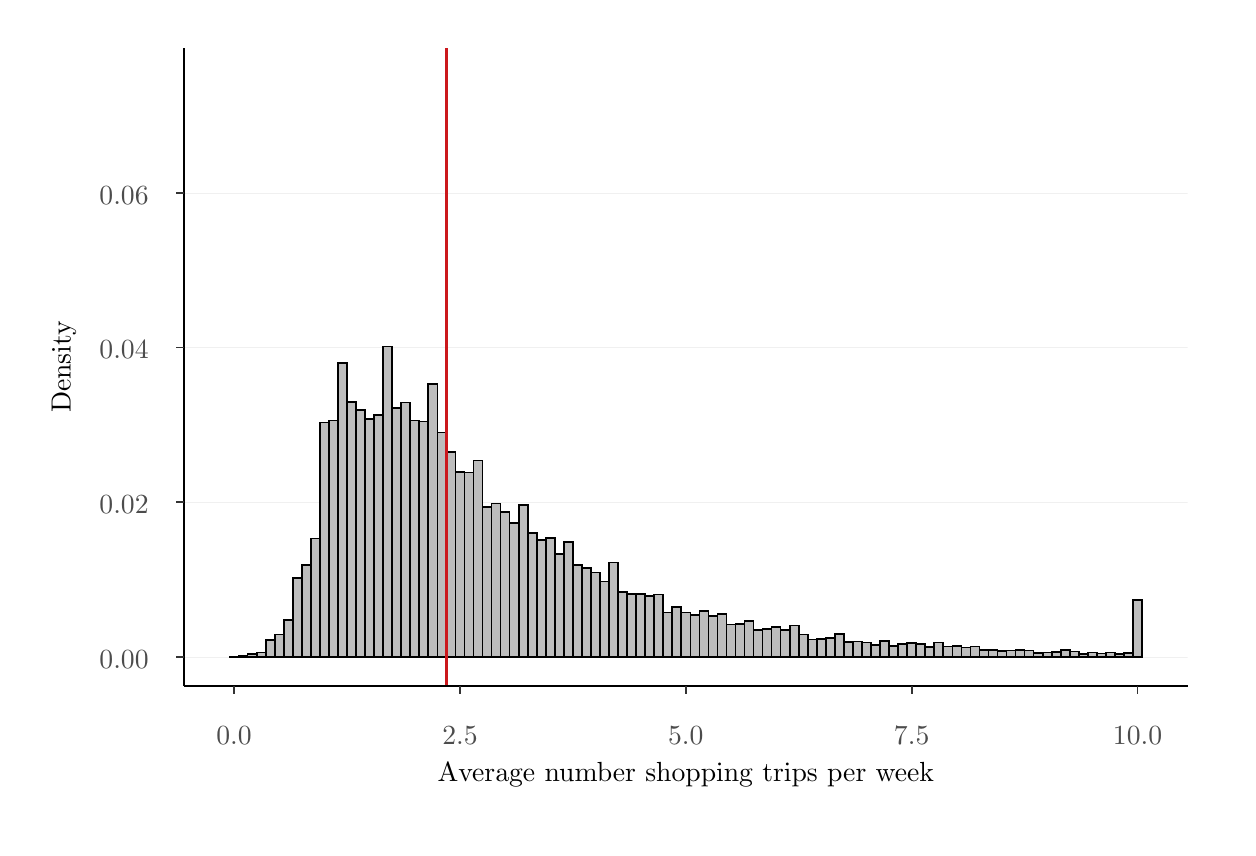
\begin{tikzpicture}[x=1pt,y=1pt]
\definecolor{fillColor}{RGB}{255,255,255}
\path[use as bounding box,fill=fillColor,fill opacity=0.00] (0,0) rectangle (433.62,289.08);
\begin{scope}
\path[clip] (  0.00,  0.00) rectangle (433.62,289.08);
\definecolor{drawColor}{RGB}{255,255,255}
\definecolor{fillColor}{RGB}{255,255,255}

\path[draw=drawColor,line width= 0.6pt,line join=round,line cap=round,fill=fillColor] ( -0.00,  0.00) rectangle (433.62,289.08);
\end{scope}
\begin{scope}
\path[clip] ( 56.47, 51.15) rectangle (419.17,281.85);
\definecolor{drawColor}{RGB}{255,255,255}

\path[draw=drawColor,line width= 0.3pt,line join=round] ( 56.47, 89.60) --
	(419.17, 89.60);

\path[draw=drawColor,line width= 0.3pt,line join=round] ( 56.47,145.53) --
	(419.17,145.53);

\path[draw=drawColor,line width= 0.3pt,line join=round] ( 56.47,201.46) --
	(419.17,201.46);

\path[draw=drawColor,line width= 0.3pt,line join=round] ( 56.47,257.38) --
	(419.17,257.38);

\path[draw=drawColor,line width= 0.3pt,line join=round] (115.39, 51.15) --
	(115.39,281.85);

\path[draw=drawColor,line width= 0.3pt,line join=round] (197.01, 51.15) --
	(197.01,281.85);

\path[draw=drawColor,line width= 0.3pt,line join=round] (278.62, 51.15) --
	(278.62,281.85);

\path[draw=drawColor,line width= 0.3pt,line join=round] (360.24, 51.15) --
	(360.24,281.85);
\definecolor{drawColor}{gray}{0.94}

\path[draw=drawColor,line width= 0.1pt,line join=round] ( 56.47, 61.64) --
	(419.17, 61.64);

\path[draw=drawColor,line width= 0.1pt,line join=round] ( 56.47,117.57) --
	(419.17,117.57);

\path[draw=drawColor,line width= 0.1pt,line join=round] ( 56.47,173.49) --
	(419.17,173.49);

\path[draw=drawColor,line width= 0.1pt,line join=round] ( 56.47,229.42) --
	(419.17,229.42);
\definecolor{drawColor}{RGB}{0,0,0}
\definecolor{fillColor}{gray}{0.74}

\path[draw=drawColor,line width= 0.6pt,line cap=rect,fill=fillColor] ( 72.95, 61.64) rectangle ( 76.22, 61.81);

\path[draw=drawColor,line width= 0.6pt,line cap=rect,fill=fillColor] ( 76.22, 61.64) rectangle ( 79.48, 62.24);

\path[draw=drawColor,line width= 0.6pt,line cap=rect,fill=fillColor] ( 79.48, 61.64) rectangle ( 82.75, 62.75);

\path[draw=drawColor,line width= 0.6pt,line cap=rect,fill=fillColor] ( 82.75, 61.64) rectangle ( 86.01, 63.35);

\path[draw=drawColor,line width= 0.6pt,line cap=rect,fill=fillColor] ( 86.01, 61.64) rectangle ( 89.28, 67.79);

\path[draw=drawColor,line width= 0.6pt,line cap=rect,fill=fillColor] ( 89.28, 61.64) rectangle ( 92.54, 69.84);

\path[draw=drawColor,line width= 0.6pt,line cap=rect,fill=fillColor] ( 92.54, 61.64) rectangle ( 95.80, 74.97);

\path[draw=drawColor,line width= 0.6pt,line cap=rect,fill=fillColor] ( 95.80, 61.64) rectangle ( 99.07, 90.26);

\path[draw=drawColor,line width= 0.6pt,line cap=rect,fill=fillColor] ( 99.07, 61.64) rectangle (102.33, 94.96);

\path[draw=drawColor,line width= 0.6pt,line cap=rect,fill=fillColor] (102.33, 61.64) rectangle (105.60,104.53);

\path[draw=drawColor,line width= 0.6pt,line cap=rect,fill=fillColor] (105.60, 61.64) rectangle (108.86,146.40);

\path[draw=drawColor,line width= 0.6pt,line cap=rect,fill=fillColor] (108.86, 61.64) rectangle (112.13,147.08);

\path[draw=drawColor,line width= 0.6pt,line cap=rect,fill=fillColor] (112.13, 61.64) rectangle (115.39,167.84);

\path[draw=drawColor,line width= 0.6pt,line cap=rect,fill=fillColor] (115.39, 61.64) rectangle (118.66,153.91);

\path[draw=drawColor,line width= 0.6pt,line cap=rect,fill=fillColor] (118.66, 61.64) rectangle (121.92,150.92);

\path[draw=drawColor,line width= 0.6pt,line cap=rect,fill=fillColor] (121.92, 61.64) rectangle (125.19,147.59);

\path[draw=drawColor,line width= 0.6pt,line cap=rect,fill=fillColor] (125.19, 61.64) rectangle (128.45,149.22);

\path[draw=drawColor,line width= 0.6pt,line cap=rect,fill=fillColor] (128.45, 61.64) rectangle (131.72,173.82);

\path[draw=drawColor,line width= 0.6pt,line cap=rect,fill=fillColor] (131.72, 61.64) rectangle (134.98,151.69);

\path[draw=drawColor,line width= 0.6pt,line cap=rect,fill=fillColor] (134.98, 61.64) rectangle (138.24,153.66);

\path[draw=drawColor,line width= 0.6pt,line cap=rect,fill=fillColor] (138.24, 61.64) rectangle (141.51,147.08);

\path[draw=drawColor,line width= 0.6pt,line cap=rect,fill=fillColor] (141.51, 61.64) rectangle (144.77,146.82);

\path[draw=drawColor,line width= 0.6pt,line cap=rect,fill=fillColor] (144.77, 61.64) rectangle (148.04,160.24);

\path[draw=drawColor,line width= 0.6pt,line cap=rect,fill=fillColor] (148.04, 61.64) rectangle (151.30,142.81);

\path[draw=drawColor,line width= 0.6pt,line cap=rect,fill=fillColor] (151.30, 61.64) rectangle (154.57,135.72);

\path[draw=drawColor,line width= 0.6pt,line cap=rect,fill=fillColor] (154.57, 61.64) rectangle (157.83,128.62);

\path[draw=drawColor,line width= 0.6pt,line cap=rect,fill=fillColor] (157.83, 61.64) rectangle (161.10,128.28);

\path[draw=drawColor,line width= 0.6pt,line cap=rect,fill=fillColor] (161.10, 61.64) rectangle (164.36,132.73);

\path[draw=drawColor,line width= 0.6pt,line cap=rect,fill=fillColor] (164.36, 61.64) rectangle (167.63,115.98);

\path[draw=drawColor,line width= 0.6pt,line cap=rect,fill=fillColor] (167.63, 61.64) rectangle (170.89,117.18);

\path[draw=drawColor,line width= 0.6pt,line cap=rect,fill=fillColor] (170.89, 61.64) rectangle (174.16,114.10);

\path[draw=drawColor,line width= 0.6pt,line cap=rect,fill=fillColor] (174.16, 61.64) rectangle (177.42,110.00);

\path[draw=drawColor,line width= 0.6pt,line cap=rect,fill=fillColor] (177.42, 61.64) rectangle (180.68,116.58);

\path[draw=drawColor,line width= 0.6pt,line cap=rect,fill=fillColor] (180.68, 61.64) rectangle (183.95,106.58);

\path[draw=drawColor,line width= 0.6pt,line cap=rect,fill=fillColor] (183.95, 61.64) rectangle (187.21,104.02);

\path[draw=drawColor,line width= 0.6pt,line cap=rect,fill=fillColor] (187.21, 61.64) rectangle (190.48,104.70);

\path[draw=drawColor,line width= 0.6pt,line cap=rect,fill=fillColor] (190.48, 61.64) rectangle (193.74, 98.89);

\path[draw=drawColor,line width= 0.6pt,line cap=rect,fill=fillColor] (193.74, 61.64) rectangle (197.01,103.25);

\path[draw=drawColor,line width= 0.6pt,line cap=rect,fill=fillColor] (197.01, 61.64) rectangle (200.27, 94.88);

\path[draw=drawColor,line width= 0.6pt,line cap=rect,fill=fillColor] (200.27, 61.64) rectangle (203.54, 93.85);

\path[draw=drawColor,line width= 0.6pt,line cap=rect,fill=fillColor] (203.54, 61.64) rectangle (206.80, 92.23);

\path[draw=drawColor,line width= 0.6pt,line cap=rect,fill=fillColor] (206.80, 61.64) rectangle (210.07, 88.98);

\path[draw=drawColor,line width= 0.6pt,line cap=rect,fill=fillColor] (210.07, 61.64) rectangle (213.33, 95.82);

\path[draw=drawColor,line width= 0.6pt,line cap=rect,fill=fillColor] (213.33, 61.64) rectangle (216.60, 85.14);

\path[draw=drawColor,line width= 0.6pt,line cap=rect,fill=fillColor] (216.60, 61.64) rectangle (219.86, 84.45);

\path[draw=drawColor,line width= 0.6pt,line cap=rect,fill=fillColor] (219.86, 61.64) rectangle (223.13, 84.37);

\path[draw=drawColor,line width= 0.6pt,line cap=rect,fill=fillColor] (223.13, 61.64) rectangle (226.39, 83.60);

\path[draw=drawColor,line width= 0.6pt,line cap=rect,fill=fillColor] (226.39, 61.64) rectangle (229.65, 84.20);

\path[draw=drawColor,line width= 0.6pt,line cap=rect,fill=fillColor] (229.65, 61.64) rectangle (232.92, 77.79);

\path[draw=drawColor,line width= 0.6pt,line cap=rect,fill=fillColor] (232.92, 61.64) rectangle (236.18, 79.67);

\path[draw=drawColor,line width= 0.6pt,line cap=rect,fill=fillColor] (236.18, 61.64) rectangle (239.45, 77.70);

\path[draw=drawColor,line width= 0.6pt,line cap=rect,fill=fillColor] (239.45, 61.64) rectangle (242.71, 76.76);

\path[draw=drawColor,line width= 0.6pt,line cap=rect,fill=fillColor] (242.71, 61.64) rectangle (245.98, 78.39);

\path[draw=drawColor,line width= 0.6pt,line cap=rect,fill=fillColor] (245.98, 61.64) rectangle (249.24, 76.51);

\path[draw=drawColor,line width= 0.6pt,line cap=rect,fill=fillColor] (249.24, 61.64) rectangle (252.51, 77.10);

\path[draw=drawColor,line width= 0.6pt,line cap=rect,fill=fillColor] (252.51, 61.64) rectangle (255.77, 73.43);

\path[draw=drawColor,line width= 0.6pt,line cap=rect,fill=fillColor] (255.77, 61.64) rectangle (259.04, 73.69);

\path[draw=drawColor,line width= 0.6pt,line cap=rect,fill=fillColor] (259.04, 61.64) rectangle (262.30, 74.63);

\path[draw=drawColor,line width= 0.6pt,line cap=rect,fill=fillColor] (262.30, 61.64) rectangle (265.57, 71.38);

\path[draw=drawColor,line width= 0.6pt,line cap=rect,fill=fillColor] (265.57, 61.64) rectangle (268.83, 71.72);

\path[draw=drawColor,line width= 0.6pt,line cap=rect,fill=fillColor] (268.83, 61.64) rectangle (272.09, 72.41);

\path[draw=drawColor,line width= 0.6pt,line cap=rect,fill=fillColor] (272.09, 61.64) rectangle (275.36, 71.38);

\path[draw=drawColor,line width= 0.6pt,line cap=rect,fill=fillColor] (275.36, 61.64) rectangle (278.62, 73.09);

\path[draw=drawColor,line width= 0.6pt,line cap=rect,fill=fillColor] (278.62, 61.64) rectangle (281.89, 69.76);

\path[draw=drawColor,line width= 0.6pt,line cap=rect,fill=fillColor] (281.89, 61.64) rectangle (285.15, 67.96);

\path[draw=drawColor,line width= 0.6pt,line cap=rect,fill=fillColor] (285.15, 61.64) rectangle (288.42, 68.22);

\path[draw=drawColor,line width= 0.6pt,line cap=rect,fill=fillColor] (288.42, 61.64) rectangle (291.68, 68.48);

\path[draw=drawColor,line width= 0.6pt,line cap=rect,fill=fillColor] (291.68, 61.64) rectangle (294.95, 70.10);

\path[draw=drawColor,line width= 0.6pt,line cap=rect,fill=fillColor] (294.95, 61.64) rectangle (298.21, 67.19);

\path[draw=drawColor,line width= 0.6pt,line cap=rect,fill=fillColor] (298.21, 61.64) rectangle (301.48, 67.28);

\path[draw=drawColor,line width= 0.6pt,line cap=rect,fill=fillColor] (301.48, 61.64) rectangle (304.74, 66.94);

\path[draw=drawColor,line width= 0.6pt,line cap=rect,fill=fillColor] (304.74, 61.64) rectangle (308.01, 66.08);

\path[draw=drawColor,line width= 0.6pt,line cap=rect,fill=fillColor] (308.01, 61.64) rectangle (311.27, 67.45);

\path[draw=drawColor,line width= 0.6pt,line cap=rect,fill=fillColor] (311.27, 61.64) rectangle (314.53, 65.57);

\path[draw=drawColor,line width= 0.6pt,line cap=rect,fill=fillColor] (314.53, 61.64) rectangle (317.80, 66.34);

\path[draw=drawColor,line width= 0.6pt,line cap=rect,fill=fillColor] (317.80, 61.64) rectangle (321.06, 66.68);

\path[draw=drawColor,line width= 0.6pt,line cap=rect,fill=fillColor] (321.06, 61.64) rectangle (324.33, 66.25);

\path[draw=drawColor,line width= 0.6pt,line cap=rect,fill=fillColor] (324.33, 61.64) rectangle (327.59, 65.40);

\path[draw=drawColor,line width= 0.6pt,line cap=rect,fill=fillColor] (327.59, 61.64) rectangle (330.86, 66.94);

\path[draw=drawColor,line width= 0.6pt,line cap=rect,fill=fillColor] (330.86, 61.64) rectangle (334.12, 65.48);

\path[draw=drawColor,line width= 0.6pt,line cap=rect,fill=fillColor] (334.12, 61.64) rectangle (337.39, 65.74);

\path[draw=drawColor,line width= 0.6pt,line cap=rect,fill=fillColor] (337.39, 61.64) rectangle (340.65, 65.14);

\path[draw=drawColor,line width= 0.6pt,line cap=rect,fill=fillColor] (340.65, 61.64) rectangle (343.92, 65.48);

\path[draw=drawColor,line width= 0.6pt,line cap=rect,fill=fillColor] (343.92, 61.64) rectangle (347.18, 64.29);

\path[draw=drawColor,line width= 0.6pt,line cap=rect,fill=fillColor] (347.18, 61.64) rectangle (350.45, 64.20);

\path[draw=drawColor,line width= 0.6pt,line cap=rect,fill=fillColor] (350.45, 61.64) rectangle (353.71, 63.86);

\path[draw=drawColor,line width= 0.6pt,line cap=rect,fill=fillColor] (353.71, 61.64) rectangle (356.97, 64.03);

\path[draw=drawColor,line width= 0.6pt,line cap=rect,fill=fillColor] (356.97, 61.64) rectangle (360.24, 64.12);

\path[draw=drawColor,line width= 0.6pt,line cap=rect,fill=fillColor] (360.24, 61.64) rectangle (363.50, 64.03);

\path[draw=drawColor,line width= 0.6pt,line cap=rect,fill=fillColor] (363.50, 61.64) rectangle (366.77, 63.01);

\path[draw=drawColor,line width= 0.6pt,line cap=rect,fill=fillColor] (366.77, 61.64) rectangle (370.03, 63.26);

\path[draw=drawColor,line width= 0.6pt,line cap=rect,fill=fillColor] (370.03, 61.64) rectangle (373.30, 63.43);

\path[draw=drawColor,line width= 0.6pt,line cap=rect,fill=fillColor] (373.30, 61.64) rectangle (376.56, 64.12);

\path[draw=drawColor,line width= 0.6pt,line cap=rect,fill=fillColor] (376.56, 61.64) rectangle (379.83, 63.61);

\path[draw=drawColor,line width= 0.6pt,line cap=rect,fill=fillColor] (379.83, 61.64) rectangle (383.09, 62.75);

\path[draw=drawColor,line width= 0.6pt,line cap=rect,fill=fillColor] (383.09, 61.64) rectangle (386.36, 63.26);

\path[draw=drawColor,line width= 0.6pt,line cap=rect,fill=fillColor] (386.36, 61.64) rectangle (389.62, 62.92);

\path[draw=drawColor,line width= 0.6pt,line cap=rect,fill=fillColor] (389.62, 61.64) rectangle (392.89, 63.26);

\path[draw=drawColor,line width= 0.6pt,line cap=rect,fill=fillColor] (392.89, 61.64) rectangle (396.15, 62.84);

\path[draw=drawColor,line width= 0.6pt,line cap=rect,fill=fillColor] (396.15, 61.64) rectangle (399.41, 63.01);

\path[draw=drawColor,line width= 0.6pt,line cap=rect,fill=fillColor] (399.41, 61.64) rectangle (402.68, 82.15);
\definecolor{drawColor}{RGB}{203,24,29}

\path[draw=drawColor,line width= 1.1pt,line join=round] (151.18, 51.15) -- (151.18,281.85);
\end{scope}
\begin{scope}
\path[clip] (  0.00,  0.00) rectangle (433.62,289.08);
\definecolor{drawColor}{RGB}{0,0,0}

\path[draw=drawColor,line width= 0.6pt,line join=round] ( 56.47, 51.15) --
	( 56.47,281.85);
\end{scope}
\begin{scope}
\path[clip] (  0.00,  0.00) rectangle (433.62,289.08);
\definecolor{drawColor}{gray}{0.30}

\node[text=drawColor,anchor=base east,inner sep=0pt, outer sep=0pt, scale=  1.00] at ( 43.72, 57.51) {0.00};

\node[text=drawColor,anchor=base east,inner sep=0pt, outer sep=0pt, scale=  1.00] at ( 43.72,113.43) {0.02};

\node[text=drawColor,anchor=base east,inner sep=0pt, outer sep=0pt, scale=  1.00] at ( 43.72,169.36) {0.04};

\node[text=drawColor,anchor=base east,inner sep=0pt, outer sep=0pt, scale=  1.00] at ( 43.72,225.29) {0.06};
\end{scope}
\begin{scope}
\path[clip] (  0.00,  0.00) rectangle (433.62,289.08);
\definecolor{drawColor}{gray}{0.20}

\path[draw=drawColor,line width= 0.6pt,line join=round] ( 53.72, 61.64) --
	( 56.47, 61.64);

\path[draw=drawColor,line width= 0.6pt,line join=round] ( 53.72,117.57) --
	( 56.47,117.57);

\path[draw=drawColor,line width= 0.6pt,line join=round] ( 53.72,173.49) --
	( 56.47,173.49);

\path[draw=drawColor,line width= 0.6pt,line join=round] ( 53.72,229.42) --
	( 56.47,229.42);
\end{scope}
\begin{scope}
\path[clip] (  0.00,  0.00) rectangle (433.62,289.08);
\definecolor{drawColor}{RGB}{0,0,0}

\path[draw=drawColor,line width= 0.6pt,line join=round] ( 56.47, 51.15) --
	(419.17, 51.15);
\end{scope}
\begin{scope}
\path[clip] (  0.00,  0.00) rectangle (433.62,289.08);
\definecolor{drawColor}{gray}{0.20}

\path[draw=drawColor,line width= 0.6pt,line join=round] ( 74.58, 48.40) --
	( 74.58, 51.15);

\path[draw=drawColor,line width= 0.6pt,line join=round] (156.20, 48.40) --
	(156.20, 51.15);

\path[draw=drawColor,line width= 0.6pt,line join=round] (237.82, 48.40) --
	(237.82, 51.15);

\path[draw=drawColor,line width= 0.6pt,line join=round] (319.43, 48.40) --
	(319.43, 51.15);

\path[draw=drawColor,line width= 0.6pt,line join=round] (401.05, 48.40) --
	(401.05, 51.15);
\end{scope}
\begin{scope}
\path[clip] (  0.00,  0.00) rectangle (433.62,289.08);
\definecolor{drawColor}{gray}{0.30}

\node[text=drawColor,anchor=base,inner sep=0pt, outer sep=0pt, scale=  1.00] at ( 74.58, 30.14) {0.0};

\node[text=drawColor,anchor=base,inner sep=0pt, outer sep=0pt, scale=  1.00] at (156.20, 30.14) {2.5};

\node[text=drawColor,anchor=base,inner sep=0pt, outer sep=0pt, scale=  1.00] at (237.82, 30.14) {5.0};

\node[text=drawColor,anchor=base,inner sep=0pt, outer sep=0pt, scale=  1.00] at (319.43, 30.14) {7.5};

\node[text=drawColor,anchor=base,inner sep=0pt, outer sep=0pt, scale=  1.00] at (401.05, 30.14) {10.0};
\end{scope}
\begin{scope}
\path[clip] (  0.00,  0.00) rectangle (433.62,289.08);
\definecolor{drawColor}{RGB}{0,0,0}

\node[text=drawColor,anchor=base,inner sep=0pt, outer sep=0pt, scale=  1.00] at (237.82, 16.79) {Average number shopping trips per week};
\end{scope}
\begin{scope}
\path[clip] (  0.00,  0.00) rectangle (433.62,289.08);
\definecolor{drawColor}{RGB}{0,0,0}

\node[text=drawColor,rotate= 90.00,anchor=base,inner sep=0pt, outer sep=0pt, scale=  1.00] at ( 15.49,166.50) {Density};
\end{scope}
\end{tikzpicture}
}
     \end{subfigure}
     \begin{subfigure}[t]{.49\textwidth}
         \centering
         \caption{France}
         \scalebox{0.45}{% Created by tikzDevice version 0.12.3.1 on 2022-07-29 15:13:47
% !TEX encoding = UTF-8 Unicode
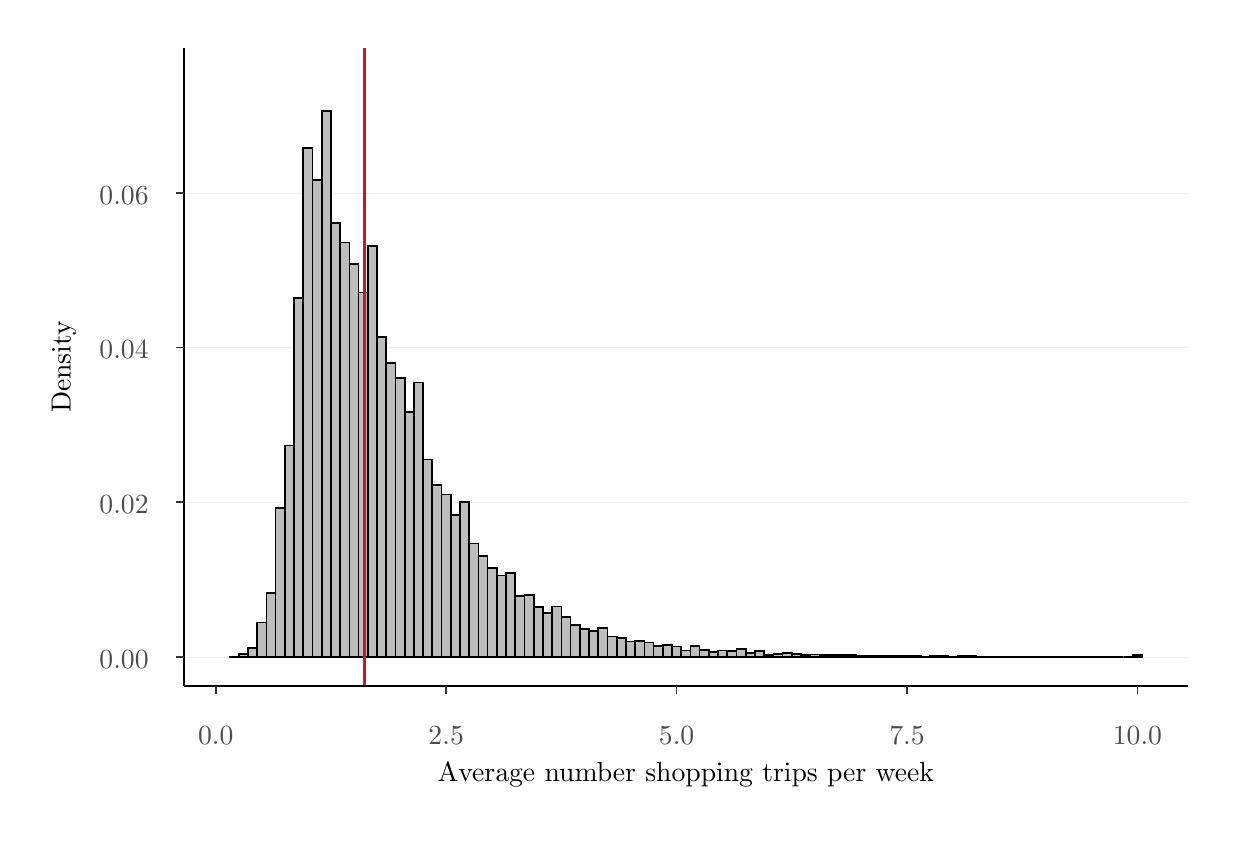
\begin{tikzpicture}[x=1pt,y=1pt]
\definecolor{fillColor}{RGB}{255,255,255}
\path[use as bounding box,fill=fillColor,fill opacity=0.00] (0,0) rectangle (433.62,289.08);
\begin{scope}
\path[clip] (  0.00,  0.00) rectangle (433.62,289.08);
\definecolor{drawColor}{RGB}{255,255,255}
\definecolor{fillColor}{RGB}{255,255,255}

\path[draw=drawColor,line width= 0.6pt,line join=round,line cap=round,fill=fillColor] ( -0.00,  0.00) rectangle (433.62,289.08);
\end{scope}
\begin{scope}
\path[clip] ( 56.47, 51.15) rectangle (419.17,281.85);
\definecolor{drawColor}{RGB}{255,255,255}

\path[draw=drawColor,line width= 0.3pt,line join=round] ( 56.47, 89.60) --
	(419.17, 89.60);

\path[draw=drawColor,line width= 0.3pt,line join=round] ( 56.47,145.53) --
	(419.17,145.53);

\path[draw=drawColor,line width= 0.3pt,line join=round] ( 56.47,201.46) --
	(419.17,201.46);

\path[draw=drawColor,line width= 0.3pt,line join=round] ( 56.47,257.38) --
	(419.17,257.38);

\path[draw=drawColor,line width= 0.3pt,line join=round] (109.59, 51.15) --
	(109.59,281.85);

\path[draw=drawColor,line width= 0.3pt,line join=round] (192.85, 51.15) --
	(192.85,281.85);

\path[draw=drawColor,line width= 0.3pt,line join=round] (276.12, 51.15) --
	(276.12,281.85);

\path[draw=drawColor,line width= 0.3pt,line join=round] (359.38, 51.15) --
	(359.38,281.85);
\definecolor{drawColor}{gray}{0.94}

\path[draw=drawColor,line width= 0.1pt,line join=round] ( 56.47, 61.64) --
	(419.17, 61.64);

\path[draw=drawColor,line width= 0.1pt,line join=round] ( 56.47,117.57) --
	(419.17,117.57);

\path[draw=drawColor,line width= 0.1pt,line join=round] ( 56.47,173.49) --
	(419.17,173.49);

\path[draw=drawColor,line width= 0.1pt,line join=round] ( 56.47,229.42) --
	(419.17,229.42);
\definecolor{drawColor}{RGB}{0,0,0}
\definecolor{fillColor}{gray}{0.74}

\path[draw=drawColor,line width= 0.6pt,line cap=rect,fill=fillColor] ( 72.95, 61.64) rectangle ( 76.28, 61.84);

\path[draw=drawColor,line width= 0.6pt,line cap=rect,fill=fillColor] ( 76.28, 61.64) rectangle ( 79.61, 62.84);

\path[draw=drawColor,line width= 0.6pt,line cap=rect,fill=fillColor] ( 79.61, 61.64) rectangle ( 82.94, 64.91);

\path[draw=drawColor,line width= 0.6pt,line cap=rect,fill=fillColor] ( 82.94, 61.64) rectangle ( 86.27, 74.12);

\path[draw=drawColor,line width= 0.6pt,line cap=rect,fill=fillColor] ( 86.27, 61.64) rectangle ( 89.61, 84.72);

\path[draw=drawColor,line width= 0.6pt,line cap=rect,fill=fillColor] ( 89.61, 61.64) rectangle ( 92.94,115.49);

\path[draw=drawColor,line width= 0.6pt,line cap=rect,fill=fillColor] ( 92.94, 61.64) rectangle ( 96.27,138.14);

\path[draw=drawColor,line width= 0.6pt,line cap=rect,fill=fillColor] ( 96.27, 61.64) rectangle ( 99.60,191.47);

\path[draw=drawColor,line width= 0.6pt,line cap=rect,fill=fillColor] ( 99.60, 61.64) rectangle (102.93,245.60);

\path[draw=drawColor,line width= 0.6pt,line cap=rect,fill=fillColor] (102.93, 61.64) rectangle (106.26,234.04);

\path[draw=drawColor,line width= 0.6pt,line cap=rect,fill=fillColor] (106.26, 61.64) rectangle (109.59,258.92);

\path[draw=drawColor,line width= 0.6pt,line cap=rect,fill=fillColor] (109.59, 61.64) rectangle (112.92,218.58);

\path[draw=drawColor,line width= 0.6pt,line cap=rect,fill=fillColor] (112.92, 61.64) rectangle (116.25,211.44);

\path[draw=drawColor,line width= 0.6pt,line cap=rect,fill=fillColor] (116.25, 61.64) rectangle (119.58,203.79);

\path[draw=drawColor,line width= 0.6pt,line cap=rect,fill=fillColor] (119.58, 61.64) rectangle (122.91,193.34);

\path[draw=drawColor,line width= 0.6pt,line cap=rect,fill=fillColor] (122.91, 61.64) rectangle (126.24,210.21);

\path[draw=drawColor,line width= 0.6pt,line cap=rect,fill=fillColor] (126.24, 61.64) rectangle (129.57,177.36);

\path[draw=drawColor,line width= 0.6pt,line cap=rect,fill=fillColor] (129.57, 61.64) rectangle (132.90,167.83);

\path[draw=drawColor,line width= 0.6pt,line cap=rect,fill=fillColor] (132.90, 61.64) rectangle (136.23,162.37);

\path[draw=drawColor,line width= 0.6pt,line cap=rect,fill=fillColor] (136.23, 61.64) rectangle (139.56,150.09);

\path[draw=drawColor,line width= 0.6pt,line cap=rect,fill=fillColor] (139.56, 61.64) rectangle (142.89,160.90);

\path[draw=drawColor,line width= 0.6pt,line cap=rect,fill=fillColor] (142.89, 61.64) rectangle (146.22,133.07);

\path[draw=drawColor,line width= 0.6pt,line cap=rect,fill=fillColor] (146.22, 61.64) rectangle (149.56,123.86);

\path[draw=drawColor,line width= 0.6pt,line cap=rect,fill=fillColor] (149.56, 61.64) rectangle (152.89,120.40);

\path[draw=drawColor,line width= 0.6pt,line cap=rect,fill=fillColor] (152.89, 61.64) rectangle (156.22,113.02);

\path[draw=drawColor,line width= 0.6pt,line cap=rect,fill=fillColor] (156.22, 61.64) rectangle (159.55,117.65);

\path[draw=drawColor,line width= 0.6pt,line cap=rect,fill=fillColor] (159.55, 61.64) rectangle (162.88,102.66);

\path[draw=drawColor,line width= 0.6pt,line cap=rect,fill=fillColor] (162.88, 61.64) rectangle (166.21, 98.23);

\path[draw=drawColor,line width= 0.6pt,line cap=rect,fill=fillColor] (166.21, 61.64) rectangle (169.54, 93.73);

\path[draw=drawColor,line width= 0.6pt,line cap=rect,fill=fillColor] (169.54, 61.64) rectangle (172.87, 91.10);

\path[draw=drawColor,line width= 0.6pt,line cap=rect,fill=fillColor] (172.87, 61.64) rectangle (176.20, 92.05);

\path[draw=drawColor,line width= 0.6pt,line cap=rect,fill=fillColor] (176.20, 61.64) rectangle (179.53, 83.64);

\path[draw=drawColor,line width= 0.6pt,line cap=rect,fill=fillColor] (179.53, 61.64) rectangle (182.86, 84.08);

\path[draw=drawColor,line width= 0.6pt,line cap=rect,fill=fillColor] (182.86, 61.64) rectangle (186.19, 79.82);

\path[draw=drawColor,line width= 0.6pt,line cap=rect,fill=fillColor] (186.19, 61.64) rectangle (189.52, 77.50);

\path[draw=drawColor,line width= 0.6pt,line cap=rect,fill=fillColor] (189.52, 61.64) rectangle (192.85, 79.90);

\path[draw=drawColor,line width= 0.6pt,line cap=rect,fill=fillColor] (192.85, 61.64) rectangle (196.18, 76.03);

\path[draw=drawColor,line width= 0.6pt,line cap=rect,fill=fillColor] (196.18, 61.64) rectangle (199.51, 73.32);

\path[draw=drawColor,line width= 0.6pt,line cap=rect,fill=fillColor] (199.51, 61.64) rectangle (202.84, 71.76);

\path[draw=drawColor,line width= 0.6pt,line cap=rect,fill=fillColor] (202.84, 61.64) rectangle (206.18, 71.09);

\path[draw=drawColor,line width= 0.6pt,line cap=rect,fill=fillColor] (206.18, 61.64) rectangle (209.51, 72.08);

\path[draw=drawColor,line width= 0.6pt,line cap=rect,fill=fillColor] (209.51, 61.64) rectangle (212.84, 69.05);

\path[draw=drawColor,line width= 0.6pt,line cap=rect,fill=fillColor] (212.84, 61.64) rectangle (216.17, 68.54);

\path[draw=drawColor,line width= 0.6pt,line cap=rect,fill=fillColor] (216.17, 61.64) rectangle (219.50, 67.26);

\path[draw=drawColor,line width= 0.6pt,line cap=rect,fill=fillColor] (219.50, 61.64) rectangle (222.83, 67.38);

\path[draw=drawColor,line width= 0.6pt,line cap=rect,fill=fillColor] (222.83, 61.64) rectangle (226.16, 66.86);

\path[draw=drawColor,line width= 0.6pt,line cap=rect,fill=fillColor] (226.16, 61.64) rectangle (229.49, 65.67);

\path[draw=drawColor,line width= 0.6pt,line cap=rect,fill=fillColor] (229.49, 61.64) rectangle (232.82, 66.10);

\path[draw=drawColor,line width= 0.6pt,line cap=rect,fill=fillColor] (232.82, 61.64) rectangle (236.15, 65.51);

\path[draw=drawColor,line width= 0.6pt,line cap=rect,fill=fillColor] (236.15, 61.64) rectangle (239.48, 64.07);

\path[draw=drawColor,line width= 0.6pt,line cap=rect,fill=fillColor] (239.48, 61.64) rectangle (242.81, 65.67);

\path[draw=drawColor,line width= 0.6pt,line cap=rect,fill=fillColor] (242.81, 61.64) rectangle (246.14, 64.19);

\path[draw=drawColor,line width= 0.6pt,line cap=rect,fill=fillColor] (246.14, 61.64) rectangle (249.47, 63.59);

\path[draw=drawColor,line width= 0.6pt,line cap=rect,fill=fillColor] (249.47, 61.64) rectangle (252.80, 64.07);

\path[draw=drawColor,line width= 0.6pt,line cap=rect,fill=fillColor] (252.80, 61.64) rectangle (256.13, 63.91);

\path[draw=drawColor,line width= 0.6pt,line cap=rect,fill=fillColor] (256.13, 61.64) rectangle (259.46, 64.47);

\path[draw=drawColor,line width= 0.6pt,line cap=rect,fill=fillColor] (259.46, 61.64) rectangle (262.80, 63.23);

\path[draw=drawColor,line width= 0.6pt,line cap=rect,fill=fillColor] (262.80, 61.64) rectangle (266.13, 63.79);

\path[draw=drawColor,line width= 0.6pt,line cap=rect,fill=fillColor] (266.13, 61.64) rectangle (269.46, 62.48);

\path[draw=drawColor,line width= 0.6pt,line cap=rect,fill=fillColor] (269.46, 61.64) rectangle (272.79, 62.64);

\path[draw=drawColor,line width= 0.6pt,line cap=rect,fill=fillColor] (272.79, 61.64) rectangle (276.12, 63.04);

\path[draw=drawColor,line width= 0.6pt,line cap=rect,fill=fillColor] (276.12, 61.64) rectangle (279.45, 62.76);

\path[draw=drawColor,line width= 0.6pt,line cap=rect,fill=fillColor] (279.45, 61.64) rectangle (282.78, 62.48);

\path[draw=drawColor,line width= 0.6pt,line cap=rect,fill=fillColor] (282.78, 61.64) rectangle (286.11, 62.52);

\path[draw=drawColor,line width= 0.6pt,line cap=rect,fill=fillColor] (286.11, 61.64) rectangle (289.44, 62.32);

\path[draw=drawColor,line width= 0.6pt,line cap=rect,fill=fillColor] (289.44, 61.64) rectangle (292.77, 62.32);

\path[draw=drawColor,line width= 0.6pt,line cap=rect,fill=fillColor] (292.77, 61.64) rectangle (296.10, 62.32);

\path[draw=drawColor,line width= 0.6pt,line cap=rect,fill=fillColor] (296.10, 61.64) rectangle (299.43, 62.36);

\path[draw=drawColor,line width= 0.6pt,line cap=rect,fill=fillColor] (299.43, 61.64) rectangle (302.76, 61.92);

\path[draw=drawColor,line width= 0.6pt,line cap=rect,fill=fillColor] (302.76, 61.64) rectangle (306.09, 62.24);

\path[draw=drawColor,line width= 0.6pt,line cap=rect,fill=fillColor] (306.09, 61.64) rectangle (309.42, 62.20);

\path[draw=drawColor,line width= 0.6pt,line cap=rect,fill=fillColor] (309.42, 61.64) rectangle (312.75, 61.92);

\path[draw=drawColor,line width= 0.6pt,line cap=rect,fill=fillColor] (312.75, 61.64) rectangle (316.08, 62.00);

\path[draw=drawColor,line width= 0.6pt,line cap=rect,fill=fillColor] (316.08, 61.64) rectangle (319.42, 61.96);

\path[draw=drawColor,line width= 0.6pt,line cap=rect,fill=fillColor] (319.42, 61.64) rectangle (322.75, 61.92);

\path[draw=drawColor,line width= 0.6pt,line cap=rect,fill=fillColor] (322.75, 61.64) rectangle (326.08, 61.76);

\path[draw=drawColor,line width= 0.6pt,line cap=rect,fill=fillColor] (326.08, 61.64) rectangle (329.41, 62.12);

\path[draw=drawColor,line width= 0.6pt,line cap=rect,fill=fillColor] (329.41, 61.64) rectangle (332.74, 62.04);

\path[draw=drawColor,line width= 0.6pt,line cap=rect,fill=fillColor] (332.74, 61.64) rectangle (336.07, 61.88);

\path[draw=drawColor,line width= 0.6pt,line cap=rect,fill=fillColor] (336.07, 61.64) rectangle (339.40, 61.92);

\path[draw=drawColor,line width= 0.6pt,line cap=rect,fill=fillColor] (339.40, 61.64) rectangle (342.73, 61.96);

\path[draw=drawColor,line width= 0.6pt,line cap=rect,fill=fillColor] (342.73, 61.64) rectangle (346.06, 61.76);

\path[draw=drawColor,line width= 0.6pt,line cap=rect,fill=fillColor] (346.06, 61.64) rectangle (349.39, 61.72);

\path[draw=drawColor,line width= 0.6pt,line cap=rect,fill=fillColor] (349.39, 61.64) rectangle (352.72, 61.84);

\path[draw=drawColor,line width= 0.6pt,line cap=rect,fill=fillColor] (352.72, 61.64) rectangle (356.05, 61.68);

\path[draw=drawColor,line width= 0.6pt,line cap=rect,fill=fillColor] (356.05, 61.64) rectangle (359.38, 61.80);

\path[draw=drawColor,line width= 0.6pt,line cap=rect,fill=fillColor] (359.38, 61.64) rectangle (362.71, 61.68);

\path[draw=drawColor,line width= 0.6pt,line cap=rect,fill=fillColor] (362.71, 61.64) rectangle (366.04, 61.68);

\path[draw=drawColor,line width= 0.6pt,line cap=rect,fill=fillColor] (366.04, 61.64) rectangle (369.37, 61.68);

\path[draw=drawColor,line width= 0.6pt,line cap=rect,fill=fillColor] (369.37, 61.64) rectangle (372.70, 61.72);

\path[draw=drawColor,line width= 0.6pt,line cap=rect,fill=fillColor] (372.70, 61.64) rectangle (376.03, 61.72);

\path[draw=drawColor,line width= 0.6pt,line cap=rect,fill=fillColor] (376.03, 61.64) rectangle (379.37, 61.72);

\path[draw=drawColor,line width= 0.6pt,line cap=rect,fill=fillColor] (379.37, 61.64) rectangle (382.70, 61.68);

\path[draw=drawColor,line width= 0.6pt,line cap=rect,fill=fillColor] (382.70, 61.64) rectangle (386.03, 61.64);

\path[draw=drawColor,line width= 0.6pt,line cap=rect,fill=fillColor] (386.03, 61.64) rectangle (389.36, 61.72);

\path[draw=drawColor,line width= 0.6pt,line cap=rect,fill=fillColor] (389.36, 61.64) rectangle (392.69, 61.68);

\path[draw=drawColor,line width= 0.6pt,line cap=rect,fill=fillColor] (392.69, 61.64) rectangle (396.02, 61.64);

\path[draw=drawColor,line width= 0.6pt,line cap=rect,fill=fillColor] (396.02, 61.64) rectangle (399.35, 61.64);

\path[draw=drawColor,line width= 0.6pt,line cap=rect,fill=fillColor] (399.35, 61.64) rectangle (402.68, 62.32);
\definecolor{drawColor}{RGB}{203,24,29}

\path[draw=drawColor,line width= 1.1pt,line join=round] (121.76, 51.15) -- (121.76,281.85);
\end{scope}
\begin{scope}
\path[clip] (  0.00,  0.00) rectangle (433.62,289.08);
\definecolor{drawColor}{RGB}{0,0,0}

\path[draw=drawColor,line width= 0.6pt,line join=round] ( 56.47, 51.15) --
	( 56.47,281.85);
\end{scope}
\begin{scope}
\path[clip] (  0.00,  0.00) rectangle (433.62,289.08);
\definecolor{drawColor}{gray}{0.30}

\node[text=drawColor,anchor=base east,inner sep=0pt, outer sep=0pt, scale=  1.00] at ( 43.72, 57.51) {0.00};

\node[text=drawColor,anchor=base east,inner sep=0pt, outer sep=0pt, scale=  1.00] at ( 43.72,113.43) {0.02};

\node[text=drawColor,anchor=base east,inner sep=0pt, outer sep=0pt, scale=  1.00] at ( 43.72,169.36) {0.04};

\node[text=drawColor,anchor=base east,inner sep=0pt, outer sep=0pt, scale=  1.00] at ( 43.72,225.29) {0.06};
\end{scope}
\begin{scope}
\path[clip] (  0.00,  0.00) rectangle (433.62,289.08);
\definecolor{drawColor}{gray}{0.20}

\path[draw=drawColor,line width= 0.6pt,line join=round] ( 53.72, 61.64) --
	( 56.47, 61.64);

\path[draw=drawColor,line width= 0.6pt,line join=round] ( 53.72,117.57) --
	( 56.47,117.57);

\path[draw=drawColor,line width= 0.6pt,line join=round] ( 53.72,173.49) --
	( 56.47,173.49);

\path[draw=drawColor,line width= 0.6pt,line join=round] ( 53.72,229.42) --
	( 56.47,229.42);
\end{scope}
\begin{scope}
\path[clip] (  0.00,  0.00) rectangle (433.62,289.08);
\definecolor{drawColor}{RGB}{0,0,0}

\path[draw=drawColor,line width= 0.6pt,line join=round] ( 56.47, 51.15) --
	(419.17, 51.15);
\end{scope}
\begin{scope}
\path[clip] (  0.00,  0.00) rectangle (433.62,289.08);
\definecolor{drawColor}{gray}{0.20}

\path[draw=drawColor,line width= 0.6pt,line join=round] ( 67.96, 48.40) --
	( 67.96, 51.15);

\path[draw=drawColor,line width= 0.6pt,line join=round] (151.22, 48.40) --
	(151.22, 51.15);

\path[draw=drawColor,line width= 0.6pt,line join=round] (234.49, 48.40) --
	(234.49, 51.15);

\path[draw=drawColor,line width= 0.6pt,line join=round] (317.75, 48.40) --
	(317.75, 51.15);

\path[draw=drawColor,line width= 0.6pt,line join=round] (401.01, 48.40) --
	(401.01, 51.15);
\end{scope}
\begin{scope}
\path[clip] (  0.00,  0.00) rectangle (433.62,289.08);
\definecolor{drawColor}{gray}{0.30}

\node[text=drawColor,anchor=base,inner sep=0pt, outer sep=0pt, scale=  1.00] at ( 67.96, 30.14) {0.0};

\node[text=drawColor,anchor=base,inner sep=0pt, outer sep=0pt, scale=  1.00] at (151.22, 30.14) {2.5};

\node[text=drawColor,anchor=base,inner sep=0pt, outer sep=0pt, scale=  1.00] at (234.49, 30.14) {5.0};

\node[text=drawColor,anchor=base,inner sep=0pt, outer sep=0pt, scale=  1.00] at (317.75, 30.14) {7.5};

\node[text=drawColor,anchor=base,inner sep=0pt, outer sep=0pt, scale=  1.00] at (401.01, 30.14) {10.0};
\end{scope}
\begin{scope}
\path[clip] (  0.00,  0.00) rectangle (433.62,289.08);
\definecolor{drawColor}{RGB}{0,0,0}

\node[text=drawColor,anchor=base,inner sep=0pt, outer sep=0pt, scale=  1.00] at (237.82, 16.79) {Average number shopping trips per week};
\end{scope}
\begin{scope}
\path[clip] (  0.00,  0.00) rectangle (433.62,289.08);
\definecolor{drawColor}{RGB}{0,0,0}

\node[text=drawColor,rotate= 90.00,anchor=base,inner sep=0pt, outer sep=0pt, scale=  1.00] at ( 15.49,166.50) {Density};
\end{scope}
\end{tikzpicture}
}
     \end{subfigure}\\
     \begin{subfigure}[t]{.49\textwidth}
         \centering
         \caption{Germany}
         \scalebox{0.45}{% Created by tikzDevice version 0.12.3.1 on 2022-07-29 15:13:47
% !TEX encoding = UTF-8 Unicode
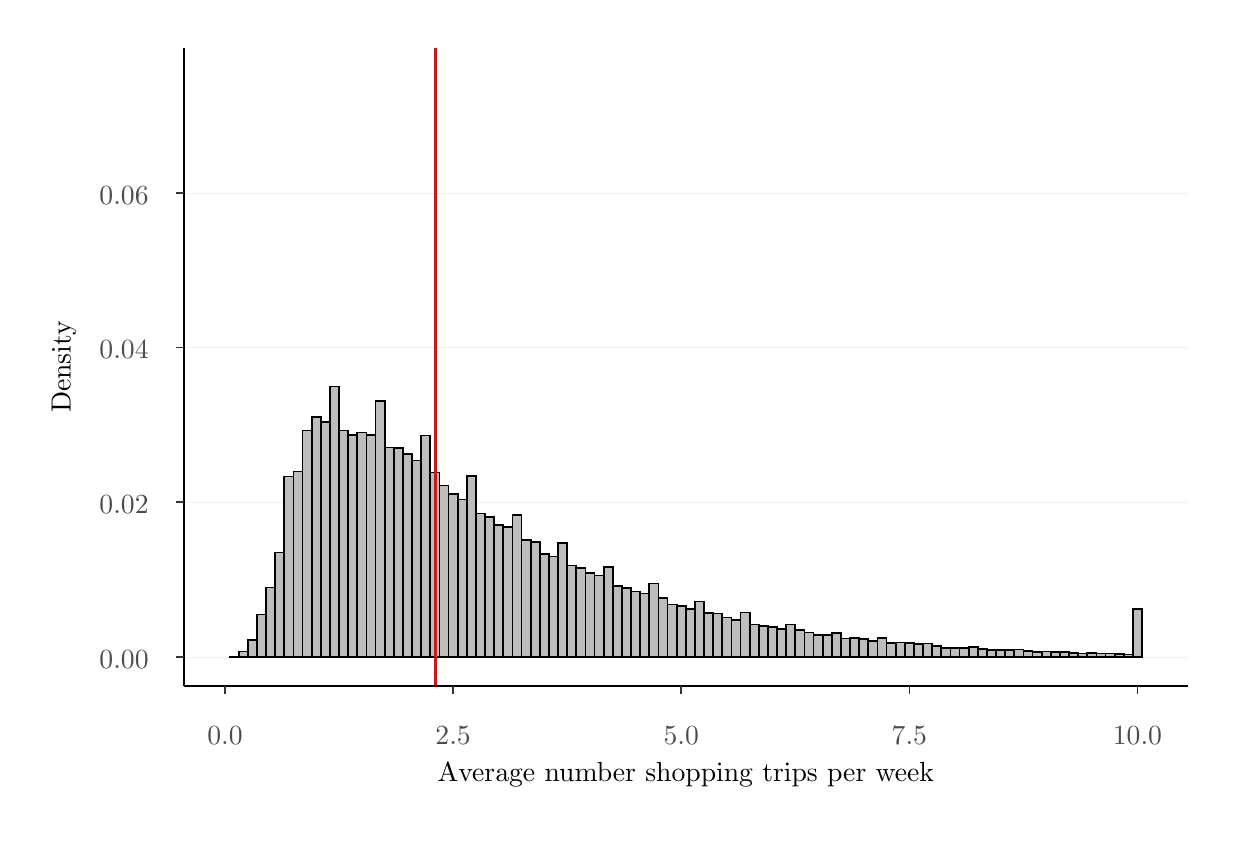
\begin{tikzpicture}[x=1pt,y=1pt]
\definecolor{fillColor}{RGB}{255,255,255}
\path[use as bounding box,fill=fillColor,fill opacity=0.00] (0,0) rectangle (433.62,289.08);
\begin{scope}
\path[clip] (  0.00,  0.00) rectangle (433.62,289.08);
\definecolor{drawColor}{RGB}{255,255,255}
\definecolor{fillColor}{RGB}{255,255,255}

\path[draw=drawColor,line width= 0.6pt,line join=round,line cap=round,fill=fillColor] ( -0.00,  0.00) rectangle (433.62,289.08);
\end{scope}
\begin{scope}
\path[clip] ( 56.47, 51.15) rectangle (419.17,281.85);
\definecolor{drawColor}{RGB}{255,255,255}

\path[draw=drawColor,line width= 0.3pt,line join=round] ( 56.47, 89.60) --
	(419.17, 89.60);

\path[draw=drawColor,line width= 0.3pt,line join=round] ( 56.47,145.53) --
	(419.17,145.53);

\path[draw=drawColor,line width= 0.3pt,line join=round] ( 56.47,201.46) --
	(419.17,201.46);

\path[draw=drawColor,line width= 0.3pt,line join=round] ( 56.47,257.38) --
	(419.17,257.38);

\path[draw=drawColor,line width= 0.3pt,line join=round] (112.52, 51.15) --
	(112.52,281.85);

\path[draw=drawColor,line width= 0.3pt,line join=round] (194.95, 51.15) --
	(194.95,281.85);

\path[draw=drawColor,line width= 0.3pt,line join=round] (277.38, 51.15) --
	(277.38,281.85);

\path[draw=drawColor,line width= 0.3pt,line join=round] (359.82, 51.15) --
	(359.82,281.85);
\definecolor{drawColor}{gray}{0.94}

\path[draw=drawColor,line width= 0.1pt,line join=round] ( 56.47, 61.64) --
	(419.17, 61.64);

\path[draw=drawColor,line width= 0.1pt,line join=round] ( 56.47,117.57) --
	(419.17,117.57);

\path[draw=drawColor,line width= 0.1pt,line join=round] ( 56.47,173.49) --
	(419.17,173.49);

\path[draw=drawColor,line width= 0.1pt,line join=round] ( 56.47,229.42) --
	(419.17,229.42);
\definecolor{drawColor}{RGB}{0,0,0}
\definecolor{fillColor}{gray}{0.74}

\path[draw=drawColor,line width= 0.6pt,line cap=rect,fill=fillColor] ( 72.95, 61.64) rectangle ( 76.25, 61.74);

\path[draw=drawColor,line width= 0.6pt,line cap=rect,fill=fillColor] ( 76.25, 61.64) rectangle ( 79.55, 63.65);

\path[draw=drawColor,line width= 0.6pt,line cap=rect,fill=fillColor] ( 79.55, 61.64) rectangle ( 82.84, 67.92);

\path[draw=drawColor,line width= 0.6pt,line cap=rect,fill=fillColor] ( 82.84, 61.64) rectangle ( 86.14, 77.04);

\path[draw=drawColor,line width= 0.6pt,line cap=rect,fill=fillColor] ( 86.14, 61.64) rectangle ( 89.44, 86.74);

\path[draw=drawColor,line width= 0.6pt,line cap=rect,fill=fillColor] ( 89.44, 61.64) rectangle ( 92.74, 99.38);

\path[draw=drawColor,line width= 0.6pt,line cap=rect,fill=fillColor] ( 92.74, 61.64) rectangle ( 96.03,126.89);

\path[draw=drawColor,line width= 0.6pt,line cap=rect,fill=fillColor] ( 96.03, 61.64) rectangle ( 99.33,128.67);

\path[draw=drawColor,line width= 0.6pt,line cap=rect,fill=fillColor] ( 99.33, 61.64) rectangle (102.63,143.49);

\path[draw=drawColor,line width= 0.6pt,line cap=rect,fill=fillColor] (102.63, 61.64) rectangle (105.92,148.32);

\path[draw=drawColor,line width= 0.6pt,line cap=rect,fill=fillColor] (105.92, 61.64) rectangle (109.22,146.53);

\path[draw=drawColor,line width= 0.6pt,line cap=rect,fill=fillColor] (109.22, 61.64) rectangle (112.52,159.41);

\path[draw=drawColor,line width= 0.6pt,line cap=rect,fill=fillColor] (112.52, 61.64) rectangle (115.82,143.56);

\path[draw=drawColor,line width= 0.6pt,line cap=rect,fill=fillColor] (115.82, 61.64) rectangle (119.11,141.79);

\path[draw=drawColor,line width= 0.6pt,line cap=rect,fill=fillColor] (119.11, 61.64) rectangle (122.41,142.82);

\path[draw=drawColor,line width= 0.6pt,line cap=rect,fill=fillColor] (122.41, 61.64) rectangle (125.71,141.87);

\path[draw=drawColor,line width= 0.6pt,line cap=rect,fill=fillColor] (125.71, 61.64) rectangle (129.01,154.23);

\path[draw=drawColor,line width= 0.6pt,line cap=rect,fill=fillColor] (129.01, 61.64) rectangle (132.30,137.39);

\path[draw=drawColor,line width= 0.6pt,line cap=rect,fill=fillColor] (132.30, 61.64) rectangle (135.60,137.11);

\path[draw=drawColor,line width= 0.6pt,line cap=rect,fill=fillColor] (135.60, 61.64) rectangle (138.90,135.06);

\path[draw=drawColor,line width= 0.6pt,line cap=rect,fill=fillColor] (138.90, 61.64) rectangle (142.19,132.70);

\path[draw=drawColor,line width= 0.6pt,line cap=rect,fill=fillColor] (142.19, 61.64) rectangle (145.49,141.77);

\path[draw=drawColor,line width= 0.6pt,line cap=rect,fill=fillColor] (145.49, 61.64) rectangle (148.79,128.35);

\path[draw=drawColor,line width= 0.6pt,line cap=rect,fill=fillColor] (148.79, 61.64) rectangle (152.09,123.67);

\path[draw=drawColor,line width= 0.6pt,line cap=rect,fill=fillColor] (152.09, 61.64) rectangle (155.38,120.49);

\path[draw=drawColor,line width= 0.6pt,line cap=rect,fill=fillColor] (155.38, 61.64) rectangle (158.68,118.58);

\path[draw=drawColor,line width= 0.6pt,line cap=rect,fill=fillColor] (158.68, 61.64) rectangle (161.98,126.96);

\path[draw=drawColor,line width= 0.6pt,line cap=rect,fill=fillColor] (161.98, 61.64) rectangle (165.28,113.48);

\path[draw=drawColor,line width= 0.6pt,line cap=rect,fill=fillColor] (165.28, 61.64) rectangle (168.57,112.33);

\path[draw=drawColor,line width= 0.6pt,line cap=rect,fill=fillColor] (168.57, 61.64) rectangle (171.87,109.44);

\path[draw=drawColor,line width= 0.6pt,line cap=rect,fill=fillColor] (171.87, 61.64) rectangle (175.17,108.64);

\path[draw=drawColor,line width= 0.6pt,line cap=rect,fill=fillColor] (175.17, 61.64) rectangle (178.46,112.97);

\path[draw=drawColor,line width= 0.6pt,line cap=rect,fill=fillColor] (178.46, 61.64) rectangle (181.76,103.83);

\path[draw=drawColor,line width= 0.6pt,line cap=rect,fill=fillColor] (181.76, 61.64) rectangle (185.06,103.28);

\path[draw=drawColor,line width= 0.6pt,line cap=rect,fill=fillColor] (185.06, 61.64) rectangle (188.36, 98.85);

\path[draw=drawColor,line width= 0.6pt,line cap=rect,fill=fillColor] (188.36, 61.64) rectangle (191.65, 97.94);

\path[draw=drawColor,line width= 0.6pt,line cap=rect,fill=fillColor] (191.65, 61.64) rectangle (194.95,102.97);

\path[draw=drawColor,line width= 0.6pt,line cap=rect,fill=fillColor] (194.95, 61.64) rectangle (198.25, 94.73);

\path[draw=drawColor,line width= 0.6pt,line cap=rect,fill=fillColor] (198.25, 61.64) rectangle (201.55, 93.83);

\path[draw=drawColor,line width= 0.6pt,line cap=rect,fill=fillColor] (201.55, 61.64) rectangle (204.84, 91.97);

\path[draw=drawColor,line width= 0.6pt,line cap=rect,fill=fillColor] (204.84, 61.64) rectangle (208.14, 91.16);

\path[draw=drawColor,line width= 0.6pt,line cap=rect,fill=fillColor] (208.14, 61.64) rectangle (211.44, 94.24);

\path[draw=drawColor,line width= 0.6pt,line cap=rect,fill=fillColor] (211.44, 61.64) rectangle (214.73, 87.22);

\path[draw=drawColor,line width= 0.6pt,line cap=rect,fill=fillColor] (214.73, 61.64) rectangle (218.03, 86.52);

\path[draw=drawColor,line width= 0.6pt,line cap=rect,fill=fillColor] (218.03, 61.64) rectangle (221.33, 85.31);

\path[draw=drawColor,line width= 0.6pt,line cap=rect,fill=fillColor] (221.33, 61.64) rectangle (224.63, 84.59);

\path[draw=drawColor,line width= 0.6pt,line cap=rect,fill=fillColor] (224.63, 61.64) rectangle (227.92, 88.17);

\path[draw=drawColor,line width= 0.6pt,line cap=rect,fill=fillColor] (227.92, 61.64) rectangle (231.22, 83.04);

\path[draw=drawColor,line width= 0.6pt,line cap=rect,fill=fillColor] (231.22, 61.64) rectangle (234.52, 80.67);

\path[draw=drawColor,line width= 0.6pt,line cap=rect,fill=fillColor] (234.52, 61.64) rectangle (237.82, 80.19);

\path[draw=drawColor,line width= 0.6pt,line cap=rect,fill=fillColor] (237.82, 61.64) rectangle (241.11, 79.04);

\path[draw=drawColor,line width= 0.6pt,line cap=rect,fill=fillColor] (241.11, 61.64) rectangle (244.41, 81.69);

\path[draw=drawColor,line width= 0.6pt,line cap=rect,fill=fillColor] (244.41, 61.64) rectangle (247.71, 77.47);

\path[draw=drawColor,line width= 0.6pt,line cap=rect,fill=fillColor] (247.71, 61.64) rectangle (251.00, 77.34);

\path[draw=drawColor,line width= 0.6pt,line cap=rect,fill=fillColor] (251.00, 61.64) rectangle (254.30, 75.98);

\path[draw=drawColor,line width= 0.6pt,line cap=rect,fill=fillColor] (254.30, 61.64) rectangle (257.60, 75.10);

\path[draw=drawColor,line width= 0.6pt,line cap=rect,fill=fillColor] (257.60, 61.64) rectangle (260.90, 77.72);

\path[draw=drawColor,line width= 0.6pt,line cap=rect,fill=fillColor] (260.90, 61.64) rectangle (264.19, 73.40);

\path[draw=drawColor,line width= 0.6pt,line cap=rect,fill=fillColor] (264.19, 61.64) rectangle (267.49, 72.97);

\path[draw=drawColor,line width= 0.6pt,line cap=rect,fill=fillColor] (267.49, 61.64) rectangle (270.79, 72.47);

\path[draw=drawColor,line width= 0.6pt,line cap=rect,fill=fillColor] (270.79, 61.64) rectangle (274.09, 71.90);

\path[draw=drawColor,line width= 0.6pt,line cap=rect,fill=fillColor] (274.09, 61.64) rectangle (277.38, 73.41);

\path[draw=drawColor,line width= 0.6pt,line cap=rect,fill=fillColor] (277.38, 61.64) rectangle (280.68, 71.33);

\path[draw=drawColor,line width= 0.6pt,line cap=rect,fill=fillColor] (280.68, 61.64) rectangle (283.98, 70.57);

\path[draw=drawColor,line width= 0.6pt,line cap=rect,fill=fillColor] (283.98, 61.64) rectangle (287.27, 69.66);

\path[draw=drawColor,line width= 0.6pt,line cap=rect,fill=fillColor] (287.27, 61.64) rectangle (290.57, 69.72);

\path[draw=drawColor,line width= 0.6pt,line cap=rect,fill=fillColor] (290.57, 61.64) rectangle (293.87, 70.31);

\path[draw=drawColor,line width= 0.6pt,line cap=rect,fill=fillColor] (293.87, 61.64) rectangle (297.17, 68.31);

\path[draw=drawColor,line width= 0.6pt,line cap=rect,fill=fillColor] (297.17, 61.64) rectangle (300.46, 68.55);

\path[draw=drawColor,line width= 0.6pt,line cap=rect,fill=fillColor] (300.46, 61.64) rectangle (303.76, 68.07);

\path[draw=drawColor,line width= 0.6pt,line cap=rect,fill=fillColor] (303.76, 61.64) rectangle (307.06, 67.47);

\path[draw=drawColor,line width= 0.6pt,line cap=rect,fill=fillColor] (307.06, 61.64) rectangle (310.36, 68.43);

\path[draw=drawColor,line width= 0.6pt,line cap=rect,fill=fillColor] (310.36, 61.64) rectangle (313.65, 66.83);

\path[draw=drawColor,line width= 0.6pt,line cap=rect,fill=fillColor] (313.65, 61.64) rectangle (316.95, 66.96);

\path[draw=drawColor,line width= 0.6pt,line cap=rect,fill=fillColor] (316.95, 61.64) rectangle (320.25, 66.72);

\path[draw=drawColor,line width= 0.6pt,line cap=rect,fill=fillColor] (320.25, 61.64) rectangle (323.55, 66.31);

\path[draw=drawColor,line width= 0.6pt,line cap=rect,fill=fillColor] (323.55, 61.64) rectangle (326.84, 66.54);

\path[draw=drawColor,line width= 0.6pt,line cap=rect,fill=fillColor] (326.84, 61.64) rectangle (330.14, 65.70);

\path[draw=drawColor,line width= 0.6pt,line cap=rect,fill=fillColor] (330.14, 61.64) rectangle (333.44, 64.98);

\path[draw=drawColor,line width= 0.6pt,line cap=rect,fill=fillColor] (333.44, 61.64) rectangle (336.73, 64.87);

\path[draw=drawColor,line width= 0.6pt,line cap=rect,fill=fillColor] (336.73, 61.64) rectangle (340.03, 64.87);

\path[draw=drawColor,line width= 0.6pt,line cap=rect,fill=fillColor] (340.03, 61.64) rectangle (343.33, 65.36);

\path[draw=drawColor,line width= 0.6pt,line cap=rect,fill=fillColor] (343.33, 61.64) rectangle (346.63, 64.45);

\path[draw=drawColor,line width= 0.6pt,line cap=rect,fill=fillColor] (346.63, 61.64) rectangle (349.92, 64.24);

\path[draw=drawColor,line width= 0.6pt,line cap=rect,fill=fillColor] (349.92, 61.64) rectangle (353.22, 64.29);

\path[draw=drawColor,line width= 0.6pt,line cap=rect,fill=fillColor] (353.22, 61.64) rectangle (356.52, 64.23);

\path[draw=drawColor,line width= 0.6pt,line cap=rect,fill=fillColor] (356.52, 61.64) rectangle (359.82, 64.43);

\path[draw=drawColor,line width= 0.6pt,line cap=rect,fill=fillColor] (359.82, 61.64) rectangle (363.11, 63.83);

\path[draw=drawColor,line width= 0.6pt,line cap=rect,fill=fillColor] (363.11, 61.64) rectangle (366.41, 63.42);

\path[draw=drawColor,line width= 0.6pt,line cap=rect,fill=fillColor] (366.41, 61.64) rectangle (369.71, 63.66);

\path[draw=drawColor,line width= 0.6pt,line cap=rect,fill=fillColor] (369.71, 61.64) rectangle (373.00, 63.36);

\path[draw=drawColor,line width= 0.6pt,line cap=rect,fill=fillColor] (373.00, 61.64) rectangle (376.30, 63.51);

\path[draw=drawColor,line width= 0.6pt,line cap=rect,fill=fillColor] (376.30, 61.64) rectangle (379.60, 63.01);

\path[draw=drawColor,line width= 0.6pt,line cap=rect,fill=fillColor] (379.60, 61.64) rectangle (382.90, 62.96);

\path[draw=drawColor,line width= 0.6pt,line cap=rect,fill=fillColor] (382.90, 61.64) rectangle (386.19, 63.07);

\path[draw=drawColor,line width= 0.6pt,line cap=rect,fill=fillColor] (386.19, 61.64) rectangle (389.49, 62.99);

\path[draw=drawColor,line width= 0.6pt,line cap=rect,fill=fillColor] (389.49, 61.64) rectangle (392.79, 62.96);

\path[draw=drawColor,line width= 0.6pt,line cap=rect,fill=fillColor] (392.79, 61.64) rectangle (396.09, 62.73);

\path[draw=drawColor,line width= 0.6pt,line cap=rect,fill=fillColor] (396.09, 61.64) rectangle (399.38, 62.57);

\path[draw=drawColor,line width= 0.6pt,line cap=rect,fill=fillColor] (399.38, 61.64) rectangle (402.68, 79.04);
\definecolor{drawColor}{RGB}{203,24,29}

\path[draw=drawColor,line width= 1.1pt,line join=round] (147.39, 51.15) -- (147.39,281.85);
\end{scope}
\begin{scope}
\path[clip] (  0.00,  0.00) rectangle (433.62,289.08);
\definecolor{drawColor}{RGB}{0,0,0}

\path[draw=drawColor,line width= 0.6pt,line join=round] ( 56.47, 51.15) --
	( 56.47,281.85);
\end{scope}
\begin{scope}
\path[clip] (  0.00,  0.00) rectangle (433.62,289.08);
\definecolor{drawColor}{gray}{0.30}

\node[text=drawColor,anchor=base east,inner sep=0pt, outer sep=0pt, scale=  1.00] at ( 43.72, 57.51) {0.00};

\node[text=drawColor,anchor=base east,inner sep=0pt, outer sep=0pt, scale=  1.00] at ( 43.72,113.43) {0.02};

\node[text=drawColor,anchor=base east,inner sep=0pt, outer sep=0pt, scale=  1.00] at ( 43.72,169.36) {0.04};

\node[text=drawColor,anchor=base east,inner sep=0pt, outer sep=0pt, scale=  1.00] at ( 43.72,225.29) {0.06};
\end{scope}
\begin{scope}
\path[clip] (  0.00,  0.00) rectangle (433.62,289.08);
\definecolor{drawColor}{gray}{0.20}

\path[draw=drawColor,line width= 0.6pt,line join=round] ( 53.72, 61.64) --
	( 56.47, 61.64);

\path[draw=drawColor,line width= 0.6pt,line join=round] ( 53.72,117.57) --
	( 56.47,117.57);

\path[draw=drawColor,line width= 0.6pt,line join=round] ( 53.72,173.49) --
	( 56.47,173.49);

\path[draw=drawColor,line width= 0.6pt,line join=round] ( 53.72,229.42) --
	( 56.47,229.42);
\end{scope}
\begin{scope}
\path[clip] (  0.00,  0.00) rectangle (433.62,289.08);
\definecolor{drawColor}{RGB}{0,0,0}

\path[draw=drawColor,line width= 0.6pt,line join=round] ( 56.47, 51.15) --
	(419.17, 51.15);
\end{scope}
\begin{scope}
\path[clip] (  0.00,  0.00) rectangle (433.62,289.08);
\definecolor{drawColor}{gray}{0.20}

\path[draw=drawColor,line width= 0.6pt,line join=round] ( 71.30, 48.40) --
	( 71.30, 51.15);

\path[draw=drawColor,line width= 0.6pt,line join=round] (153.74, 48.40) --
	(153.74, 51.15);

\path[draw=drawColor,line width= 0.6pt,line join=round] (236.17, 48.40) --
	(236.17, 51.15);

\path[draw=drawColor,line width= 0.6pt,line join=round] (318.60, 48.40) --
	(318.60, 51.15);

\path[draw=drawColor,line width= 0.6pt,line join=round] (401.03, 48.40) --
	(401.03, 51.15);
\end{scope}
\begin{scope}
\path[clip] (  0.00,  0.00) rectangle (433.62,289.08);
\definecolor{drawColor}{gray}{0.30}

\node[text=drawColor,anchor=base,inner sep=0pt, outer sep=0pt, scale=  1.00] at ( 71.30, 30.14) {0.0};

\node[text=drawColor,anchor=base,inner sep=0pt, outer sep=0pt, scale=  1.00] at (153.74, 30.14) {2.5};

\node[text=drawColor,anchor=base,inner sep=0pt, outer sep=0pt, scale=  1.00] at (236.17, 30.14) {5.0};

\node[text=drawColor,anchor=base,inner sep=0pt, outer sep=0pt, scale=  1.00] at (318.60, 30.14) {7.5};

\node[text=drawColor,anchor=base,inner sep=0pt, outer sep=0pt, scale=  1.00] at (401.03, 30.14) {10.0};
\end{scope}
\begin{scope}
\path[clip] (  0.00,  0.00) rectangle (433.62,289.08);
\definecolor{drawColor}{RGB}{0,0,0}

\node[text=drawColor,anchor=base,inner sep=0pt, outer sep=0pt, scale=  1.00] at (237.82, 16.79) {Average number shopping trips per week};
\end{scope}
\begin{scope}
\path[clip] (  0.00,  0.00) rectangle (433.62,289.08);
\definecolor{drawColor}{RGB}{0,0,0}

\node[text=drawColor,rotate= 90.00,anchor=base,inner sep=0pt, outer sep=0pt, scale=  1.00] at ( 15.49,166.50) {Density};
\end{scope}
\end{tikzpicture}
}
     \end{subfigure}
     \begin{subfigure}[t]{.49\textwidth}
         \centering
         \caption{The Netherlands}
         \scalebox{0.45}{% Created by tikzDevice version 0.12.3.1 on 2022-07-29 15:13:47
% !TEX encoding = UTF-8 Unicode
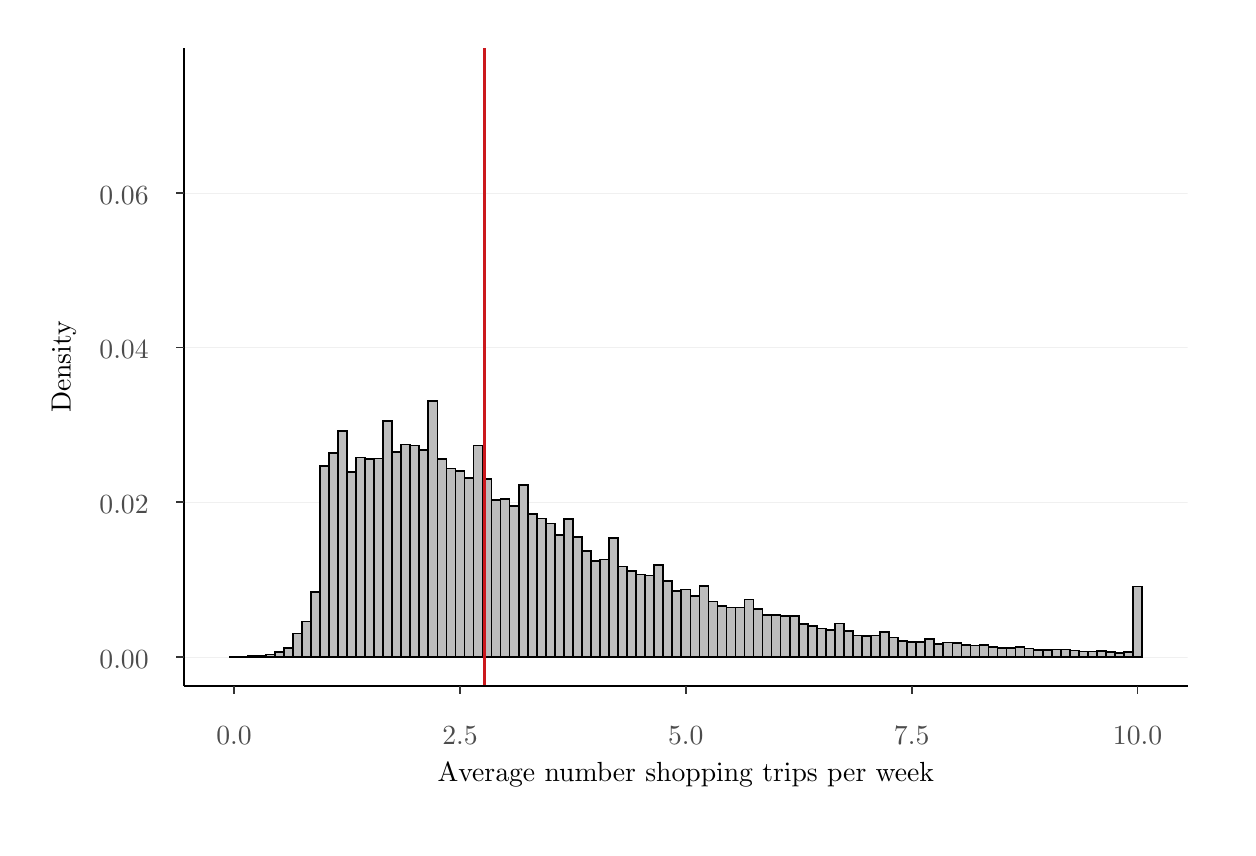
\begin{tikzpicture}[x=1pt,y=1pt]
\definecolor{fillColor}{RGB}{255,255,255}
\path[use as bounding box,fill=fillColor,fill opacity=0.00] (0,0) rectangle (433.62,289.08);
\begin{scope}
\path[clip] (  0.00,  0.00) rectangle (433.62,289.08);
\definecolor{drawColor}{RGB}{255,255,255}
\definecolor{fillColor}{RGB}{255,255,255}

\path[draw=drawColor,line width= 0.6pt,line join=round,line cap=round,fill=fillColor] ( -0.00,  0.00) rectangle (433.62,289.08);
\end{scope}
\begin{scope}
\path[clip] ( 56.47, 51.15) rectangle (419.17,281.85);
\definecolor{drawColor}{RGB}{255,255,255}

\path[draw=drawColor,line width= 0.3pt,line join=round] ( 56.47, 89.60) --
	(419.17, 89.60);

\path[draw=drawColor,line width= 0.3pt,line join=round] ( 56.47,145.53) --
	(419.17,145.53);

\path[draw=drawColor,line width= 0.3pt,line join=round] ( 56.47,201.46) --
	(419.17,201.46);

\path[draw=drawColor,line width= 0.3pt,line join=round] ( 56.47,257.38) --
	(419.17,257.38);

\path[draw=drawColor,line width= 0.3pt,line join=round] (115.39, 51.15) --
	(115.39,281.85);

\path[draw=drawColor,line width= 0.3pt,line join=round] (197.01, 51.15) --
	(197.01,281.85);

\path[draw=drawColor,line width= 0.3pt,line join=round] (278.62, 51.15) --
	(278.62,281.85);

\path[draw=drawColor,line width= 0.3pt,line join=round] (360.24, 51.15) --
	(360.24,281.85);
\definecolor{drawColor}{gray}{0.94}

\path[draw=drawColor,line width= 0.1pt,line join=round] ( 56.47, 61.64) --
	(419.17, 61.64);

\path[draw=drawColor,line width= 0.1pt,line join=round] ( 56.47,117.57) --
	(419.17,117.57);

\path[draw=drawColor,line width= 0.1pt,line join=round] ( 56.47,173.49) --
	(419.17,173.49);

\path[draw=drawColor,line width= 0.1pt,line join=round] ( 56.47,229.42) --
	(419.17,229.42);
\definecolor{drawColor}{RGB}{0,0,0}
\definecolor{fillColor}{gray}{0.74}

\path[draw=drawColor,line width= 0.6pt,line cap=rect,fill=fillColor] ( 72.95, 61.64) rectangle ( 76.22, 61.67);

\path[draw=drawColor,line width= 0.6pt,line cap=rect,fill=fillColor] ( 76.22, 61.64) rectangle ( 79.48, 61.74);

\path[draw=drawColor,line width= 0.6pt,line cap=rect,fill=fillColor] ( 79.48, 61.64) rectangle ( 82.75, 61.94);

\path[draw=drawColor,line width= 0.6pt,line cap=rect,fill=fillColor] ( 82.75, 61.64) rectangle ( 86.01, 62.04);

\path[draw=drawColor,line width= 0.6pt,line cap=rect,fill=fillColor] ( 86.01, 61.64) rectangle ( 89.28, 62.53);

\path[draw=drawColor,line width= 0.6pt,line cap=rect,fill=fillColor] ( 89.28, 61.64) rectangle ( 92.54, 63.59);

\path[draw=drawColor,line width= 0.6pt,line cap=rect,fill=fillColor] ( 92.54, 61.64) rectangle ( 95.80, 65.01);

\path[draw=drawColor,line width= 0.6pt,line cap=rect,fill=fillColor] ( 95.80, 61.64) rectangle ( 99.07, 70.19);

\path[draw=drawColor,line width= 0.6pt,line cap=rect,fill=fillColor] ( 99.07, 61.64) rectangle (102.33, 74.55);

\path[draw=drawColor,line width= 0.6pt,line cap=rect,fill=fillColor] (102.33, 61.64) rectangle (105.60, 85.15);

\path[draw=drawColor,line width= 0.6pt,line cap=rect,fill=fillColor] (105.60, 61.64) rectangle (108.86,130.72);

\path[draw=drawColor,line width= 0.6pt,line cap=rect,fill=fillColor] (108.86, 61.64) rectangle (112.13,135.32);

\path[draw=drawColor,line width= 0.6pt,line cap=rect,fill=fillColor] (112.13, 61.64) rectangle (115.39,143.37);

\path[draw=drawColor,line width= 0.6pt,line cap=rect,fill=fillColor] (115.39, 61.64) rectangle (118.66,128.41);

\path[draw=drawColor,line width= 0.6pt,line cap=rect,fill=fillColor] (118.66, 61.64) rectangle (121.92,133.70);

\path[draw=drawColor,line width= 0.6pt,line cap=rect,fill=fillColor] (121.92, 61.64) rectangle (125.19,133.17);

\path[draw=drawColor,line width= 0.6pt,line cap=rect,fill=fillColor] (125.19, 61.64) rectangle (128.45,133.37);

\path[draw=drawColor,line width= 0.6pt,line cap=rect,fill=fillColor] (128.45, 61.64) rectangle (131.72,146.94);

\path[draw=drawColor,line width= 0.6pt,line cap=rect,fill=fillColor] (131.72, 61.64) rectangle (134.98,135.84);

\path[draw=drawColor,line width= 0.6pt,line cap=rect,fill=fillColor] (134.98, 61.64) rectangle (138.24,138.42);

\path[draw=drawColor,line width= 0.6pt,line cap=rect,fill=fillColor] (138.24, 61.64) rectangle (141.51,138.09);

\path[draw=drawColor,line width= 0.6pt,line cap=rect,fill=fillColor] (141.51, 61.64) rectangle (144.77,136.57);

\path[draw=drawColor,line width= 0.6pt,line cap=rect,fill=fillColor] (144.77, 61.64) rectangle (148.04,154.14);

\path[draw=drawColor,line width= 0.6pt,line cap=rect,fill=fillColor] (148.04, 61.64) rectangle (151.30,133.10);

\path[draw=drawColor,line width= 0.6pt,line cap=rect,fill=fillColor] (151.30, 61.64) rectangle (154.57,129.73);

\path[draw=drawColor,line width= 0.6pt,line cap=rect,fill=fillColor] (154.57, 61.64) rectangle (157.83,128.91);

\path[draw=drawColor,line width= 0.6pt,line cap=rect,fill=fillColor] (157.83, 61.64) rectangle (161.10,126.33);

\path[draw=drawColor,line width= 0.6pt,line cap=rect,fill=fillColor] (161.10, 61.64) rectangle (164.36,138.09);

\path[draw=drawColor,line width= 0.6pt,line cap=rect,fill=fillColor] (164.36, 61.64) rectangle (167.63,126.04);

\path[draw=drawColor,line width= 0.6pt,line cap=rect,fill=fillColor] (167.63, 61.64) rectangle (170.89,118.37);

\path[draw=drawColor,line width= 0.6pt,line cap=rect,fill=fillColor] (170.89, 61.64) rectangle (174.16,118.80);

\path[draw=drawColor,line width= 0.6pt,line cap=rect,fill=fillColor] (174.16, 61.64) rectangle (177.42,116.23);

\path[draw=drawColor,line width= 0.6pt,line cap=rect,fill=fillColor] (177.42, 61.64) rectangle (180.68,123.76);

\path[draw=drawColor,line width= 0.6pt,line cap=rect,fill=fillColor] (180.68, 61.64) rectangle (183.95,113.42);

\path[draw=drawColor,line width= 0.6pt,line cap=rect,fill=fillColor] (183.95, 61.64) rectangle (187.21,111.67);

\path[draw=drawColor,line width= 0.6pt,line cap=rect,fill=fillColor] (187.21, 61.64) rectangle (190.48,109.89);

\path[draw=drawColor,line width= 0.6pt,line cap=rect,fill=fillColor] (190.48, 61.64) rectangle (193.74,105.79);

\path[draw=drawColor,line width= 0.6pt,line cap=rect,fill=fillColor] (193.74, 61.64) rectangle (197.01,111.51);

\path[draw=drawColor,line width= 0.6pt,line cap=rect,fill=fillColor] (197.01, 61.64) rectangle (200.27,104.97);

\path[draw=drawColor,line width= 0.6pt,line cap=rect,fill=fillColor] (200.27, 61.64) rectangle (203.54,100.08);

\path[draw=drawColor,line width= 0.6pt,line cap=rect,fill=fillColor] (203.54, 61.64) rectangle (206.80, 96.45);

\path[draw=drawColor,line width= 0.6pt,line cap=rect,fill=fillColor] (206.80, 61.64) rectangle (210.07, 96.91);

\path[draw=drawColor,line width= 0.6pt,line cap=rect,fill=fillColor] (210.07, 61.64) rectangle (213.33,104.70);

\path[draw=drawColor,line width= 0.6pt,line cap=rect,fill=fillColor] (213.33, 61.64) rectangle (216.60, 94.37);

\path[draw=drawColor,line width= 0.6pt,line cap=rect,fill=fillColor] (216.60, 61.64) rectangle (219.86, 92.65);

\path[draw=drawColor,line width= 0.6pt,line cap=rect,fill=fillColor] (219.86, 61.64) rectangle (223.13, 91.49);

\path[draw=drawColor,line width= 0.6pt,line cap=rect,fill=fillColor] (223.13, 61.64) rectangle (226.39, 91.13);

\path[draw=drawColor,line width= 0.6pt,line cap=rect,fill=fillColor] (226.39, 61.64) rectangle (229.65, 94.99);

\path[draw=drawColor,line width= 0.6pt,line cap=rect,fill=fillColor] (229.65, 61.64) rectangle (232.92, 89.15);

\path[draw=drawColor,line width= 0.6pt,line cap=rect,fill=fillColor] (232.92, 61.64) rectangle (236.18, 85.61);

\path[draw=drawColor,line width= 0.6pt,line cap=rect,fill=fillColor] (236.18, 61.64) rectangle (239.45, 86.01);

\path[draw=drawColor,line width= 0.6pt,line cap=rect,fill=fillColor] (239.45, 61.64) rectangle (242.71, 83.70);

\path[draw=drawColor,line width= 0.6pt,line cap=rect,fill=fillColor] (242.71, 61.64) rectangle (245.98, 87.43);

\path[draw=drawColor,line width= 0.6pt,line cap=rect,fill=fillColor] (245.98, 61.64) rectangle (249.24, 81.69);

\path[draw=drawColor,line width= 0.6pt,line cap=rect,fill=fillColor] (249.24, 61.64) rectangle (252.51, 80.17);

\path[draw=drawColor,line width= 0.6pt,line cap=rect,fill=fillColor] (252.51, 61.64) rectangle (255.77, 79.57);

\path[draw=drawColor,line width= 0.6pt,line cap=rect,fill=fillColor] (255.77, 61.64) rectangle (259.04, 79.51);

\path[draw=drawColor,line width= 0.6pt,line cap=rect,fill=fillColor] (259.04, 61.64) rectangle (262.30, 82.51);

\path[draw=drawColor,line width= 0.6pt,line cap=rect,fill=fillColor] (262.30, 61.64) rectangle (265.57, 79.01);

\path[draw=drawColor,line width= 0.6pt,line cap=rect,fill=fillColor] (265.57, 61.64) rectangle (268.83, 76.73);

\path[draw=drawColor,line width= 0.6pt,line cap=rect,fill=fillColor] (268.83, 61.64) rectangle (272.09, 76.90);

\path[draw=drawColor,line width= 0.6pt,line cap=rect,fill=fillColor] (272.09, 61.64) rectangle (275.36, 76.57);

\path[draw=drawColor,line width= 0.6pt,line cap=rect,fill=fillColor] (275.36, 61.64) rectangle (278.62, 76.43);

\path[draw=drawColor,line width= 0.6pt,line cap=rect,fill=fillColor] (278.62, 61.64) rectangle (281.89, 73.53);

\path[draw=drawColor,line width= 0.6pt,line cap=rect,fill=fillColor] (281.89, 61.64) rectangle (285.15, 72.97);

\path[draw=drawColor,line width= 0.6pt,line cap=rect,fill=fillColor] (285.15, 61.64) rectangle (288.42, 71.98);

\path[draw=drawColor,line width= 0.6pt,line cap=rect,fill=fillColor] (288.42, 61.64) rectangle (291.68, 71.41);

\path[draw=drawColor,line width= 0.6pt,line cap=rect,fill=fillColor] (291.68, 61.64) rectangle (294.95, 73.83);

\path[draw=drawColor,line width= 0.6pt,line cap=rect,fill=fillColor] (294.95, 61.64) rectangle (298.21, 71.05);

\path[draw=drawColor,line width= 0.6pt,line cap=rect,fill=fillColor] (298.21, 61.64) rectangle (301.48, 69.47);

\path[draw=drawColor,line width= 0.6pt,line cap=rect,fill=fillColor] (301.48, 61.64) rectangle (304.74, 69.20);

\path[draw=drawColor,line width= 0.6pt,line cap=rect,fill=fillColor] (304.74, 61.64) rectangle (308.01, 69.47);

\path[draw=drawColor,line width= 0.6pt,line cap=rect,fill=fillColor] (308.01, 61.64) rectangle (311.27, 70.79);

\path[draw=drawColor,line width= 0.6pt,line cap=rect,fill=fillColor] (311.27, 61.64) rectangle (314.53, 68.74);

\path[draw=drawColor,line width= 0.6pt,line cap=rect,fill=fillColor] (314.53, 61.64) rectangle (317.80, 67.52);

\path[draw=drawColor,line width= 0.6pt,line cap=rect,fill=fillColor] (317.80, 61.64) rectangle (321.06, 67.12);

\path[draw=drawColor,line width= 0.6pt,line cap=rect,fill=fillColor] (321.06, 61.64) rectangle (324.33, 67.19);

\path[draw=drawColor,line width= 0.6pt,line cap=rect,fill=fillColor] (324.33, 61.64) rectangle (327.59, 68.24);

\path[draw=drawColor,line width= 0.6pt,line cap=rect,fill=fillColor] (327.59, 61.64) rectangle (330.86, 66.40);

\path[draw=drawColor,line width= 0.6pt,line cap=rect,fill=fillColor] (330.86, 61.64) rectangle (334.12, 66.86);

\path[draw=drawColor,line width= 0.6pt,line cap=rect,fill=fillColor] (334.12, 61.64) rectangle (337.39, 66.73);

\path[draw=drawColor,line width= 0.6pt,line cap=rect,fill=fillColor] (337.39, 61.64) rectangle (340.65, 66.07);

\path[draw=drawColor,line width= 0.6pt,line cap=rect,fill=fillColor] (340.65, 61.64) rectangle (343.92, 65.83);

\path[draw=drawColor,line width= 0.6pt,line cap=rect,fill=fillColor] (343.92, 61.64) rectangle (347.18, 66.00);

\path[draw=drawColor,line width= 0.6pt,line cap=rect,fill=fillColor] (347.18, 61.64) rectangle (350.45, 65.24);

\path[draw=drawColor,line width= 0.6pt,line cap=rect,fill=fillColor] (350.45, 61.64) rectangle (353.71, 64.91);

\path[draw=drawColor,line width= 0.6pt,line cap=rect,fill=fillColor] (353.71, 61.64) rectangle (356.97, 64.88);

\path[draw=drawColor,line width= 0.6pt,line cap=rect,fill=fillColor] (356.97, 61.64) rectangle (360.24, 65.37);

\path[draw=drawColor,line width= 0.6pt,line cap=rect,fill=fillColor] (360.24, 61.64) rectangle (363.50, 64.71);

\path[draw=drawColor,line width= 0.6pt,line cap=rect,fill=fillColor] (363.50, 61.64) rectangle (366.77, 64.25);

\path[draw=drawColor,line width= 0.6pt,line cap=rect,fill=fillColor] (366.77, 61.64) rectangle (370.03, 64.22);

\path[draw=drawColor,line width= 0.6pt,line cap=rect,fill=fillColor] (370.03, 61.64) rectangle (373.30, 64.35);

\path[draw=drawColor,line width= 0.6pt,line cap=rect,fill=fillColor] (373.30, 61.64) rectangle (376.56, 64.38);

\path[draw=drawColor,line width= 0.6pt,line cap=rect,fill=fillColor] (376.56, 61.64) rectangle (379.83, 64.08);

\path[draw=drawColor,line width= 0.6pt,line cap=rect,fill=fillColor] (379.83, 61.64) rectangle (383.09, 63.65);

\path[draw=drawColor,line width= 0.6pt,line cap=rect,fill=fillColor] (383.09, 61.64) rectangle (386.36, 63.62);

\path[draw=drawColor,line width= 0.6pt,line cap=rect,fill=fillColor] (386.36, 61.64) rectangle (389.62, 63.92);

\path[draw=drawColor,line width= 0.6pt,line cap=rect,fill=fillColor] (389.62, 61.64) rectangle (392.89, 63.49);

\path[draw=drawColor,line width= 0.6pt,line cap=rect,fill=fillColor] (392.89, 61.64) rectangle (396.15, 63.06);

\path[draw=drawColor,line width= 0.6pt,line cap=rect,fill=fillColor] (396.15, 61.64) rectangle (399.41, 63.49);

\path[draw=drawColor,line width= 0.6pt,line cap=rect,fill=fillColor] (399.41, 61.64) rectangle (402.68, 87.17);
\definecolor{drawColor}{RGB}{203,24,29}

\path[draw=drawColor,line width= 1.1pt,line join=round] (164.99, 51.15) -- (164.99,281.85);
\end{scope}
\begin{scope}
\path[clip] (  0.00,  0.00) rectangle (433.62,289.08);
\definecolor{drawColor}{RGB}{0,0,0}

\path[draw=drawColor,line width= 0.6pt,line join=round] ( 56.47, 51.15) --
	( 56.47,281.85);
\end{scope}
\begin{scope}
\path[clip] (  0.00,  0.00) rectangle (433.62,289.08);
\definecolor{drawColor}{gray}{0.30}

\node[text=drawColor,anchor=base east,inner sep=0pt, outer sep=0pt, scale=  1.00] at ( 43.72, 57.51) {0.00};

\node[text=drawColor,anchor=base east,inner sep=0pt, outer sep=0pt, scale=  1.00] at ( 43.72,113.43) {0.02};

\node[text=drawColor,anchor=base east,inner sep=0pt, outer sep=0pt, scale=  1.00] at ( 43.72,169.36) {0.04};

\node[text=drawColor,anchor=base east,inner sep=0pt, outer sep=0pt, scale=  1.00] at ( 43.72,225.29) {0.06};
\end{scope}
\begin{scope}
\path[clip] (  0.00,  0.00) rectangle (433.62,289.08);
\definecolor{drawColor}{gray}{0.20}

\path[draw=drawColor,line width= 0.6pt,line join=round] ( 53.72, 61.64) --
	( 56.47, 61.64);

\path[draw=drawColor,line width= 0.6pt,line join=round] ( 53.72,117.57) --
	( 56.47,117.57);

\path[draw=drawColor,line width= 0.6pt,line join=round] ( 53.72,173.49) --
	( 56.47,173.49);

\path[draw=drawColor,line width= 0.6pt,line join=round] ( 53.72,229.42) --
	( 56.47,229.42);
\end{scope}
\begin{scope}
\path[clip] (  0.00,  0.00) rectangle (433.62,289.08);
\definecolor{drawColor}{RGB}{0,0,0}

\path[draw=drawColor,line width= 0.6pt,line join=round] ( 56.47, 51.15) --
	(419.17, 51.15);
\end{scope}
\begin{scope}
\path[clip] (  0.00,  0.00) rectangle (433.62,289.08);
\definecolor{drawColor}{gray}{0.20}

\path[draw=drawColor,line width= 0.6pt,line join=round] ( 74.58, 48.40) --
	( 74.58, 51.15);

\path[draw=drawColor,line width= 0.6pt,line join=round] (156.20, 48.40) --
	(156.20, 51.15);

\path[draw=drawColor,line width= 0.6pt,line join=round] (237.82, 48.40) --
	(237.82, 51.15);

\path[draw=drawColor,line width= 0.6pt,line join=round] (319.43, 48.40) --
	(319.43, 51.15);

\path[draw=drawColor,line width= 0.6pt,line join=round] (401.05, 48.40) --
	(401.05, 51.15);
\end{scope}
\begin{scope}
\path[clip] (  0.00,  0.00) rectangle (433.62,289.08);
\definecolor{drawColor}{gray}{0.30}

\node[text=drawColor,anchor=base,inner sep=0pt, outer sep=0pt, scale=  1.00] at ( 74.58, 30.14) {0.0};

\node[text=drawColor,anchor=base,inner sep=0pt, outer sep=0pt, scale=  1.00] at (156.20, 30.14) {2.5};

\node[text=drawColor,anchor=base,inner sep=0pt, outer sep=0pt, scale=  1.00] at (237.82, 30.14) {5.0};

\node[text=drawColor,anchor=base,inner sep=0pt, outer sep=0pt, scale=  1.00] at (319.43, 30.14) {7.5};

\node[text=drawColor,anchor=base,inner sep=0pt, outer sep=0pt, scale=  1.00] at (401.05, 30.14) {10.0};
\end{scope}
\begin{scope}
\path[clip] (  0.00,  0.00) rectangle (433.62,289.08);
\definecolor{drawColor}{RGB}{0,0,0}

\node[text=drawColor,anchor=base,inner sep=0pt, outer sep=0pt, scale=  1.00] at (237.82, 16.79) {Average number shopping trips per week};
\end{scope}
\begin{scope}
\path[clip] (  0.00,  0.00) rectangle (433.62,289.08);
\definecolor{drawColor}{RGB}{0,0,0}

\node[text=drawColor,rotate= 90.00,anchor=base,inner sep=0pt, outer sep=0pt, scale=  1.00] at ( 15.49,166.50) {Density};
\end{scope}
\end{tikzpicture}
}
     \end{subfigure}
     \parbox{\textwidth}{
        \begin{spacing}{1} 
            {\footnotesize 
            \textit{Notes}: These figures plot the distribution of the average number of store visits barcodes per week across households in the final sample on the 68 included product categories for each country. We define a store visit as a combination of visiting a store on a certain day. Hence, visiting two different stores on the same day is counted as two store visits.}
        \end{spacing}}
 \end{figure} 


\subsection{Stores}
\begin{table}[H]
	\centering		
	\caption{Stores: Overview}
    \label{tab: app_data_stores_overview}
	\begin{spacing}{1.1}
        \scalebox{0.97}{
        \begin{tabular}{lrrrrrrrr} \toprule
            &   \multicolumn{2}{c}{Belgium} & \multicolumn{2}{c}{France} & 
                \multicolumn{2}{c}{Germany} & \multicolumn{2}{c}{Netherlands} 
                \\ \cmidrule(lr){2-3} \cmidrule(lr){4-5} \cmidrule(lr){6-7} \cmidrule(lr){8-9} 
            Store & Sales & Trans & Sales & Trans & Sales & Trans & Sales & Trans\\ \midrule
		    Grocery store&0.38&0.38&0.82&0.80&0.42&0.41&0.60&0.61\\
Discounter&0.44&0.49&0.11&0.15&0.39&0.48&0.28&0.32\\
Convenience store&0.02&0.03&0.02&0.03&0.02&0.01&0.01&0.01\\
Specialist store&0.12&0.09&0.03&0.01&0.17&0.11&0.10&0.05\\
Excluded&0.03&0.03&0.01&0.01&0.00&0.00&0.01&0.01\\
\bottomrule

	    \end{tabular}}
    \end{spacing}
    \parbox{\textwidth}{
        \begin{spacing}{1} 
            {\footnotesize 
            \textit{Notes}: This table shows for each country the expenditure and transaction share across the different stores respectively.}
        \end{spacing}}
\end{table}